% Options for packages loaded elsewhere
\PassOptionsToPackage{unicode}{hyperref}
\PassOptionsToPackage{hyphens}{url}
%
\documentclass[
]{article}
\usepackage{amsmath,amssymb}
\usepackage{lmodern}
\usepackage{iftex}
\ifPDFTeX
  \usepackage[T1]{fontenc}
  \usepackage[utf8]{inputenc}
  \usepackage{textcomp} % provide euro and other symbols
\else % if luatex or xetex
  \usepackage{unicode-math}
  \defaultfontfeatures{Scale=MatchLowercase}
  \defaultfontfeatures[\rmfamily]{Ligatures=TeX,Scale=1}
\fi
% Use upquote if available, for straight quotes in verbatim environments
\IfFileExists{upquote.sty}{\usepackage{upquote}}{}
\IfFileExists{microtype.sty}{% use microtype if available
  \usepackage[]{microtype}
  \UseMicrotypeSet[protrusion]{basicmath} % disable protrusion for tt fonts
}{}
\makeatletter
\@ifundefined{KOMAClassName}{% if non-KOMA class
  \IfFileExists{parskip.sty}{%
    \usepackage{parskip}
  }{% else
    \setlength{\parindent}{0pt}
    \setlength{\parskip}{6pt plus 2pt minus 1pt}}
}{% if KOMA class
  \KOMAoptions{parskip=half}}
\makeatother
\usepackage{xcolor}
\usepackage{graphicx}
\makeatletter
\def\maxwidth{\ifdim\Gin@nat@width>\linewidth\linewidth\else\Gin@nat@width\fi}
\def\maxheight{\ifdim\Gin@nat@height>\textheight\textheight\else\Gin@nat@height\fi}
\makeatother
% Scale images if necessary, so that they will not overflow the page
% margins by default, and it is still possible to overwrite the defaults
% using explicit options in \includegraphics[width, height, ...]{}
\setkeys{Gin}{width=\maxwidth,height=\maxheight,keepaspectratio}
% Set default figure placement to htbp
\makeatletter
\def\fps@figure{htbp}
\makeatother
\usepackage[normalem]{ulem}
\setlength{\emergencystretch}{3em} % prevent overfull lines
\providecommand{\tightlist}{%
  \setlength{\itemsep}{0pt}\setlength{\parskip}{0pt}}
\setcounter{secnumdepth}{-\maxdimen} % remove section numbering
\ifLuaTeX
  \usepackage{selnolig}  % disable illegal ligatures
\fi
\IfFileExists{bookmark.sty}{\usepackage{bookmark}}{\usepackage{hyperref}}
\IfFileExists{xurl.sty}{\usepackage{xurl}}{} % add URL line breaks if available
\urlstyle{same} % disable monospaced font for URLs
\hypersetup{
  hidelinks,
  pdfcreator={LaTeX via pandoc}}

\author{}
\date{}

\begin{document}

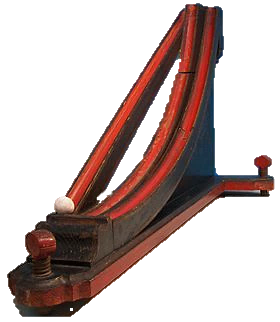
\includegraphics[width=4.38889in,height=4.57292in]{Imagenes/media/image1.png}

\begin{quote}
\emph{Haz de la ciencia no el camino para entender el universo, sino la
manera de comprender de dónde venimos y hacia dónde vamos.}
\end{quote}

\textbf{Índice}

\textbf{CAPÍTULO 1: CINEMÁTICA EN COORDENADAS GENERALIZADAS}

\begin{itemize}
\item
  \begin{quote}
  Cinemática en Coordenadas Cartesianas 1
  \end{quote}
\item
  \begin{quote}
  Cinemática en Coordenadas Cilíndricas 6
  \end{quote}
\item
  \begin{quote}
  Cinemática en Coordenadas Esféricas 12
  \end{quote}
\item
  \begin{quote}
  Cinemática en Coordenadas Curvilíneas 17
  \end{quote}
\item
  \begin{quote}
  Ejemplos 26
  \end{quote}
\end{itemize}

\textbf{CAPÍTULO 2: DINÁMICA DE LAGRANGE}

\begin{itemize}
\item
  \begin{quote}
  Deducción de la Ecuación de Movimiento de Lagrange 29
  \end{quote}
\item
  \begin{quote}
  Fuerzas de Ligadura y Ecuaciones de Superficies 31
  \end{quote}
\item
  \begin{quote}
  Principio de los Trabajos Virtuales 33
  \end{quote}
\item
  \begin{quote}
  Ejemplos 37
  \end{quote}
\item
  \begin{quote}
  Principio de Mínima Acción 52
  \end{quote}
\item
  \begin{quote}
  Ejemplos 60
  \end{quote}
\item
  \begin{quote}
  Problema de la Braquistócrona 65
  \end{quote}
\end{itemize}

\textbf{CAPÍTULO 3: FUERZAS DE TIPO CENTRAL}

\begin{itemize}
\item
  \begin{quote}
  Lagrangiano de un Sistema de dos Partículas 70
  \end{quote}
\item
  \begin{quote}
  Teoremas de Conservación, Primera y Segunda Ley de Kepler 72
  \end{quote}
\item
  \begin{quote}
  Ecuación Diferencial para Determinar el Tipo de Órbita 78
  \end{quote}
\item
  \begin{quote}
  Partícula Bajo la Acción de una Fuerza de un Fuerza de Tipo Central 80
  \end{quote}
\item
  \begin{quote}
  Teorema del Virial y Tercera Ley de Kepler 86
  \end{quote}
\item
  \begin{quote}
  Ejemplos 94
  \end{quote}
\end{itemize}

\textbf{CAPÍTULO 4: TEORÍA DE DISPERSIÓN Y CHOQUES ELÁSTICOS}

\begin{itemize}
\item
  \begin{quote}
  Teoría de Dispersión 98
  \end{quote}
\item
  \begin{quote}
  Dispersión de una Partícula que Viaja desde el Infinito bajo la
  \end{quote}
\end{itemize}

\begin{quote}
Acción de una Fuerza de Tipo Central 117
\end{quote}

\begin{itemize}
\item
  \begin{quote}
  Experimento de Rutherford 120
  \end{quote}
\end{itemize}

\textbf{CAPÍTULO 5: DINÁMICA DE HAMILTON}

\begin{itemize}
\item
  \begin{quote}
  Propiedades de Simetría 127
  \end{quote}
\item
  \begin{quote}
  Ecuaciones de Movimiento Hamilton 132
  \end{quote}
\item
  \begin{quote}
  Principio de Mínima Acción de Hamilton Modificado 133
  \end{quote}
\item
  \begin{quote}
  Ejemplos 135
  \end{quote}
\item
  \begin{quote}
  Solución Routhiana de un Sistema Dinámico 144
  \end{quote}
\item
  \begin{quote}
  Corchetes de Poisson y Álgebra de Lie 154
  \end{quote}
\item
  \begin{quote}
  Ejemplos 156
  \end{quote}
\item
  \begin{quote}
  Ecuación de Hamilton-Jacobi 158
  \end{quote}
\item
  \begin{quote}
  Ejemplo 161
  \end{quote}
\item
  \begin{quote}
  Deducción de la Ecuación de Schrödinger Mediante la Ecuación
  \end{quote}
\end{itemize}

\begin{quote}
De Hamilton-Jacobi 162
\end{quote}

\textbf{Capítulo 1 Cinemática en Coordenadas Generalizadas}

Dentro del marco del desarrollo de la mecánica es indispensable tener
claridad del concepto de \emph{punto} o \emph{punto puntiforme.} Esta
noción se puede entender como aquél punto material que no ocupa lugar en
el espacio que aparece de la necesidad de describir el movimiento de un
cuerpo bajo ciertas condiciones. Se puede citar el ejemplo de un sólido
rígido, este se puede considerar como un punto material cuando no se
está haciendo la descripción sobre su eje, en otros términos las
condiciones pueden cambiar.

En mecánica, cuando se trata de obtener los observables descritos por un
sistema es necesario definir un sistema de coordenadas; en esencia,
dicho sistema de coordenadas es definido como un sistema inercial.

En este primer capítulo se va a hacer un tratamiento a partir de los
sistemas de coordenadas ya conocidos para luego llevarlos a una
generalidad y obtener las coordenadas generalizadas, donde se llega a
mostrar que las coordenadas ya conocidas son un caso particular de las
coordenadas generalizadas.

\textbf{CINEMÁTICA EN COORDENADAS CARTESIANAS}

Considérese el sistema de referencia mostrado en la \emph{figura 1}:

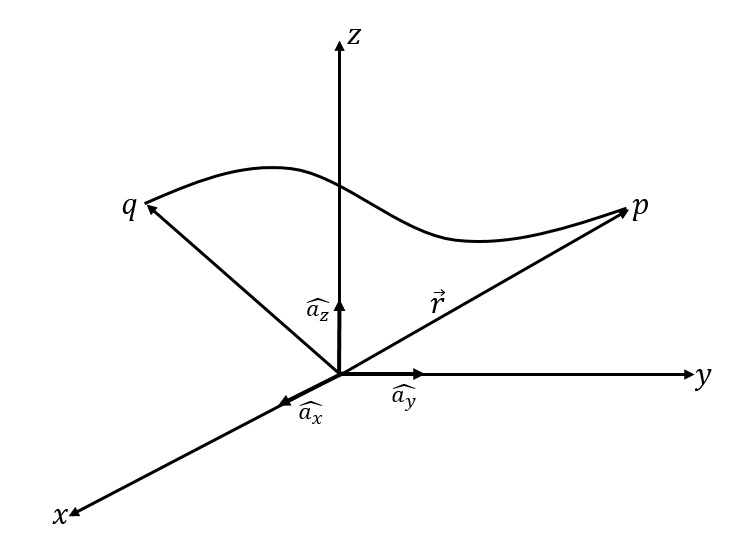
\includegraphics[width=5.57431in,height=4in]{Imagenes/media/image2.jpeg}

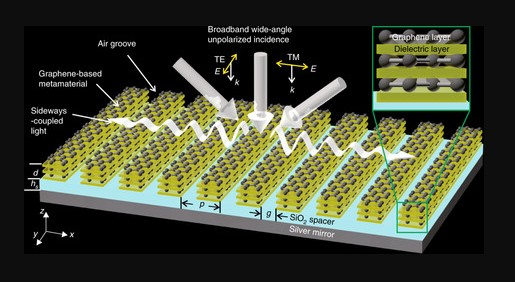
\includegraphics[width=5.36528in,height=2.93264in]{Imagenes/media/image3.jpeg}

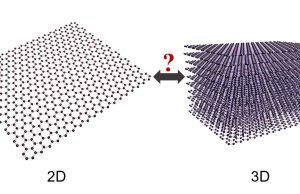
\includegraphics[width=4.16346in,height=2.69052in]{Imagenes/media/image4.jpeg}

Grafeno

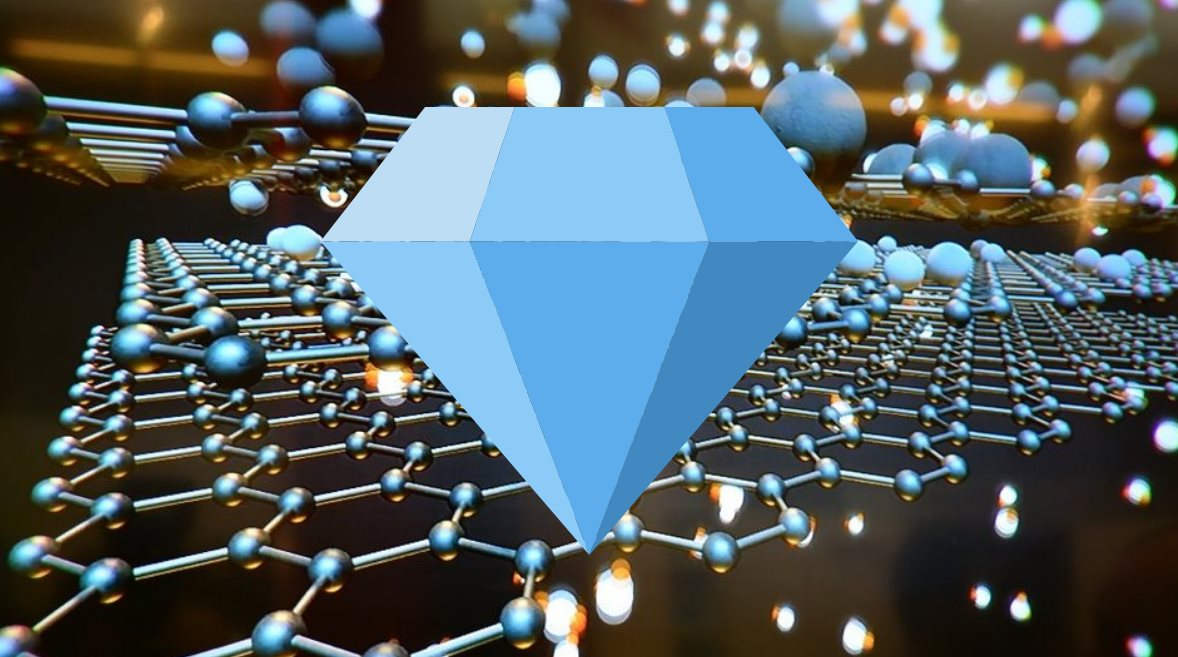
\includegraphics[width=4.82529in,height=2.69231in]{Imagenes/media/image5.jpeg}

Diamante sintético

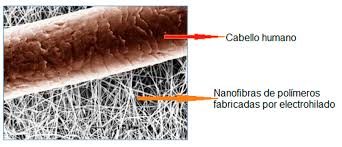
\includegraphics[width=4.72115in,height=2.31638in]{Imagenes/media/image6.jpeg}

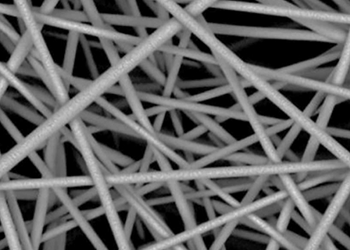
\includegraphics[width=3.64444in,height=2.60556in]{Imagenes/media/image7.png}

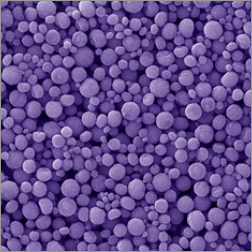
\includegraphics[width=2.26923in,height=2.26923in]{Imagenes/media/image8.png}

TiO\textsubscript{2}

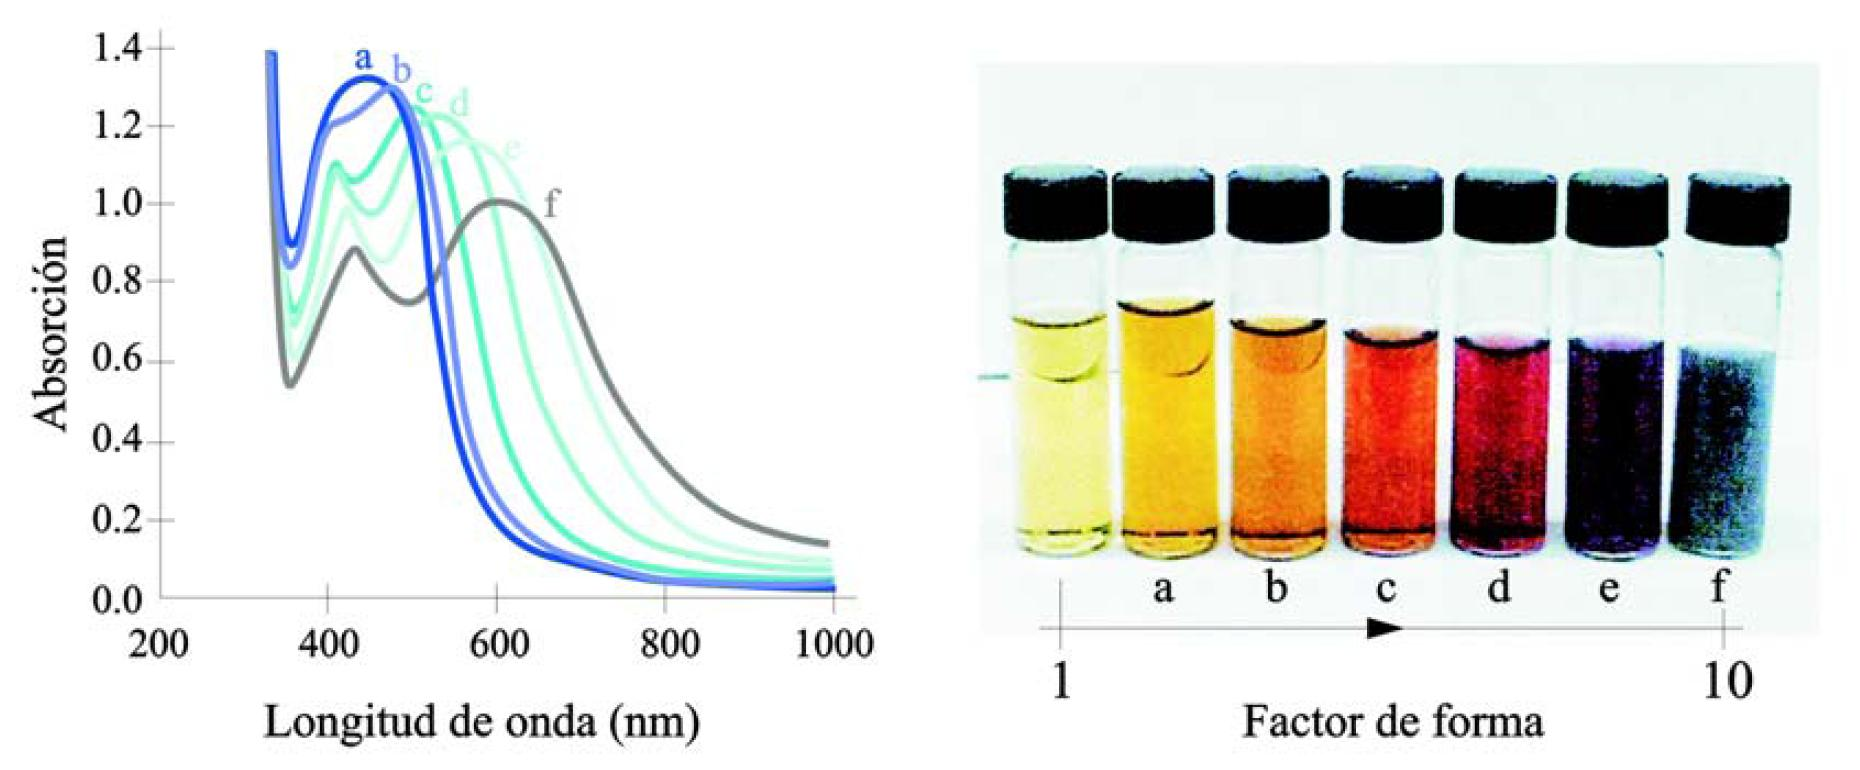
\includegraphics[width=5.66185in,height=2.34348in]{Imagenes/media/image9.jpeg}

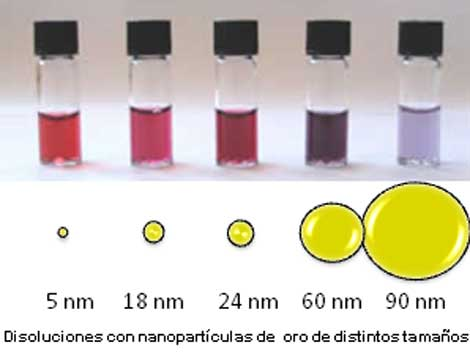
\includegraphics[width=3.48063in,height=2.63961in]{Imagenes/media/image10.jpeg}

Nanopartículas de oro

En el sistema de referencia mostrado anteriormente se utiliza la base
\((\widehat{a_{x},}\ \widehat{a_{y},}\ \widehat{a_{z}})\) de vectores
unitarios de donde se define el vector posición:

\(\overrightarrow{r}(x,y,z) = x\widehat{a_{x}} + y\widehat{a_{y}} + z\widehat{a_{z}}\ \ \ \ \ \)(1)

De donde se puede ver que \(\overrightarrow{r}\) es un punto en el
espacio. Si se considera que la partícula se mueve en un parámetro de
evolución \(t + \mathrm{\Delta}t\) o de cambio en las coordenadas, el
vector posición toma la siguiente forma:

\(\overrightarrow{r}(t) = \overrightarrow{r}(x,\ y,\ z;\ t)\) (2)

Una vez tenido en cuenta el parámetro de evolución \(t\); se tiene:

\(\overrightarrow{r}(x,\ y,\ z;\ t) = x(t)\widehat{a_{x}} + y(t)\widehat{a_{y}} + z(t)\widehat{a_{z}}\)
(3)

De donde se pueden ver las ecuaciones paramétricas de la trayectoria:

\[x = x(t)\]

\[y = y(t)\]

\[z = z(t)\]

Al tener las nuevas coordenadas, el vector posición evaluado en
\(t + \mathrm{\Delta}t\) es:

\(\overrightarrow{r}(x,\ y,\ z;\ t + \mathrm{\Delta}t) = {\overrightarrow{r}}_{f}\left( x_{f},\ y_{f},\ z_{f};\ t_{f} \right) = x(t + \mathrm{\Delta}t)\widehat{a_{x}} + y(t + \mathrm{\Delta}t)\widehat{a_{y}} + z(t + \mathrm{\Delta}t)\widehat{a_{z}}\)
(4)

\[\overrightarrow{r} + \mathrm{\Delta}\overrightarrow{r} = {\overrightarrow{r}}_{f}\]

\[\mathrm{\Delta}\overrightarrow{r} = {\overrightarrow{r}}_{f} - \overrightarrow{r}\]

\(\mathrm{\Delta}\overrightarrow{r} = \left\lbrack \ x(t + \mathrm{\Delta}t) - x(t) \right\rbrack\widehat{a_{x}} + \left\lbrack \ y(t + \mathrm{\Delta}t) - y(t) \right\rbrack\widehat{a_{y}} + \left\lbrack \ z(t + \mathrm{\Delta}t) - z(t) \right\rbrack\widehat{a_{z}}\)
(5)

Es de notar que en la ecuación (5),
\(\mathrm{\Delta}\overrightarrow{r}\) representa un cambio del vector
posición que es independiente de la trayectoria, muestra un punto
inicial y una función final descrita por la partícula.

La razón de cambio del desplazamiento por intervalo de tiempo es
denominada \emph{velocidad media.} Se entiende la velocidad media como
vector, puesto que es el resultado de dividir una magnitud vectorial
sobre una magnitud escalar.

Gráficamente se deduce dicha magnitud de la siguiente manera:

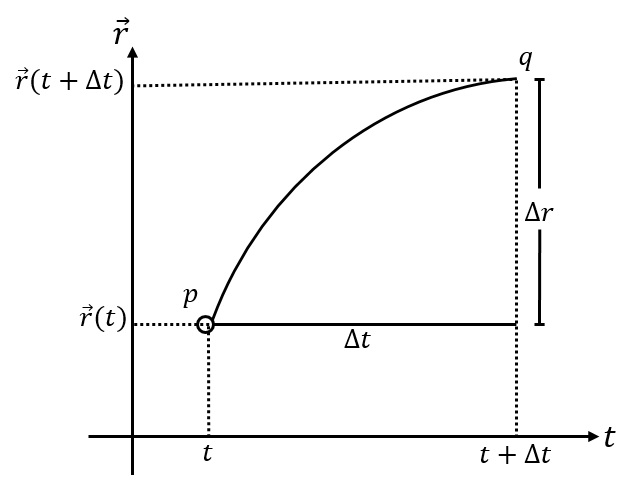
\includegraphics[width=4.96528in,height=3.72917in]{Imagenes/media/image11.jpeg}
A partir de la \emph{figura 2} se tiene que la velocidad media está dada
por:

\[\overrightarrow{v} = \frac{\mathrm{\Delta}\overrightarrow{r}}{\mathrm{\Delta}t}\]

Esto es;

\[\overrightarrow{v} = \frac{\left\lbrack \ x(t + \mathrm{\Delta}t) - x(t) \right\rbrack\widehat{a_{x}}}{\mathrm{\Delta}t} + \frac{\left\lbrack \ y(t + \mathrm{\Delta}t) - y(t) \right\rbrack\widehat{a_{y}}}{\mathrm{\Delta}t} + \frac{\left\lbrack \ z(t + \mathrm{\Delta}t) - z(t) \right\rbrack\widehat{a_{z}}}{\mathrm{\Delta}t}\]

Geométricamente la ecuación (6) conlleva a la siguiente interpretación:
\textbf{la velocidad media es el vector de la pendiente de la recta
secante que corta a la trayectoria en los puntos} \(\mathbf{p}\)
\textbf{y} \(\mathbf{q}\)\textbf{.}

Así mismo se define la velocidad instantánea como:

\[\frac{d\overrightarrow{r}}{dt} = \lim_{\mathrm{\Delta}t \rightarrow 0}\frac{\left\lbrack \ x(t + \mathrm{\Delta}t) - x(t) \right\rbrack\widehat{a_{x}} + \left\lbrack \ y(t + \mathrm{\Delta}t) - y(t) \right\rbrack\widehat{a_{y}} + \left\lbrack \ z(t + \mathrm{\Delta}t) - z(t) \right\rbrack\widehat{a_{z}}}{\mathrm{\Delta}t}\]

La expresión (7) brinda \textbf{el valor de la pendiente de la recta
tangente que corta a la trayectoria en un solo punto.}

\[\overrightarrow{v} = \frac{d\overrightarrow{r}}{dt} = \frac{dx}{dt}\widehat{a_{x}} + \frac{dy}{dt}\widehat{a_{y}} + \frac{dz}{dt}\widehat{a_{z}}\]

\[\overrightarrow{v} = \dot{x}\widehat{a_{x}} + \dot{y}\widehat{a_{y}} + \dot{z}\widehat{a_{z}}\]

De esta manera \(\overrightarrow{v}\) es la razón de cambio del vector
posición por unidad de tiempo.

Análogamente se puede mostrar que:

\[\overrightarrow{a} = \frac{d\overrightarrow{\dot{r}}}{dt} = \frac{d^{2}\overrightarrow{r}}{dt^{2}}\]

La prueba se deja como ejercicio. \(\therefore\)

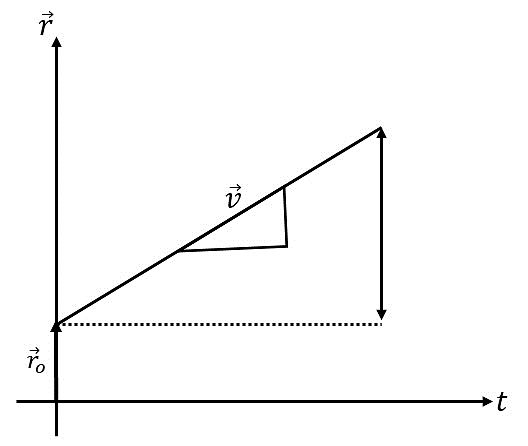
\includegraphics[width=3.38681in,height=3.61458in]{Imagenes/media/image12.png}Ahora
se procede a analizar el M.R.U, de donde se tiene que
\(\overrightarrow{v} = cte\); así:

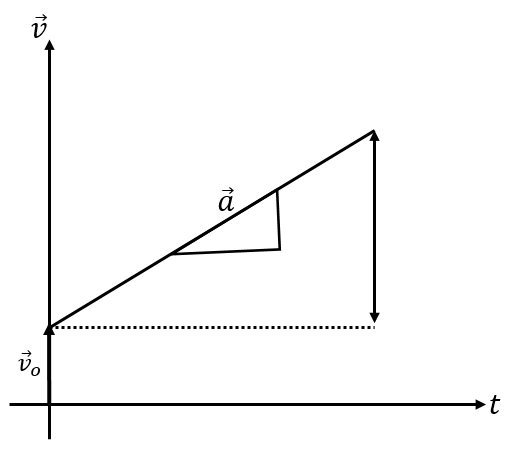
\includegraphics[width=3.27222in,height=3.58333in]{Imagenes/media/image13.png}Haciendo
un tratamiento similar para el M.R.U.A donde
\(\overrightarrow{a} = cte\); se tiene que:

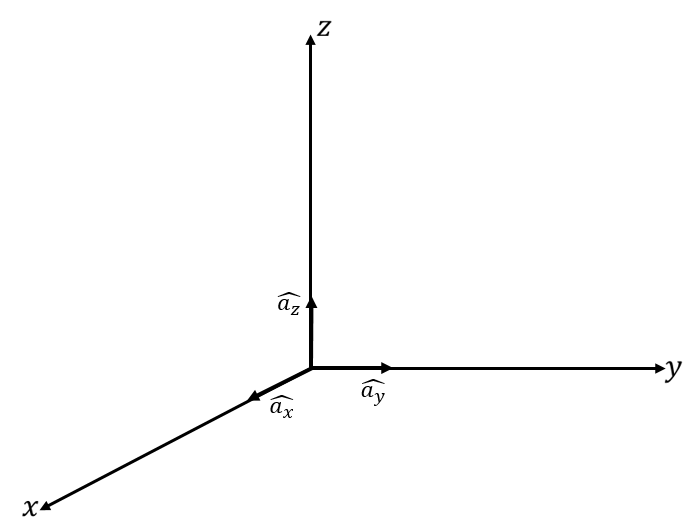
\includegraphics[width=6.08333in,height=4.56389in]{Imagenes/media/image14.png}Todo
este tratamiento de cinemática es obtenido por medio de una base de
vectores unitarios en coordenadas cartesianas (ver \emph{figura 5}).

Recuerde que un vector unitario es aquél que posee norma uno y tiene la
dirección en que crece el eje ordenado, de esta manera:

\[\widehat{a_{x}} \bullet \widehat{a_{x}} = \widehat{a_{y}} \bullet \widehat{a_{y}} = \widehat{a_{z}} \bullet \widehat{a_{z}} = 1\]

\[\widehat{a_{x}} \bullet \widehat{a_{y}} = 0 \rightarrow \widehat{a_{x}}\bot\widehat{a_{y}}\]

\[\widehat{a_{x}} \bullet \widehat{a_{z}} = 0 \rightarrow \widehat{a_{x}}\bot\widehat{a_{z}}\]

\[\widehat{a_{y}} \bullet \widehat{a_{z}} = 0 \rightarrow \widehat{a_{y}}\bot\widehat{a_{z}}\]

Si se introduce el \emph{delta de Kronecker} se tiene entonces:

\[\widehat{a_{i}} \bullet \widehat{a_{j}} = \delta_{ij} = \left\{ \begin{matrix}
0\ \ \ \ \ \ i \neq j \\
1\ \ \ \ \ \ i = j \\
\end{matrix} \right.\ \]

\textbf{Si} \(\mathbf{i \neq j}\) \textbf{se tiene una base ortonormal.}

\textbf{Si} \(\mathbf{i = j}\) \textbf{se tiene una base fija.}

\textbf{Si}
\(\widehat{\mathbf{a}_{\mathbf{i}}}\mathbf{\bullet}\widehat{\mathbf{a}_{\mathbf{j}}}\mathbf{=}\mathbf{\delta}_{\mathbf{ij}}\)
\textbf{se tiene una base ortonormal móvil.}

\textbf{CINEMÁTICA EN COORDENADAS CILÍNDRICAS}

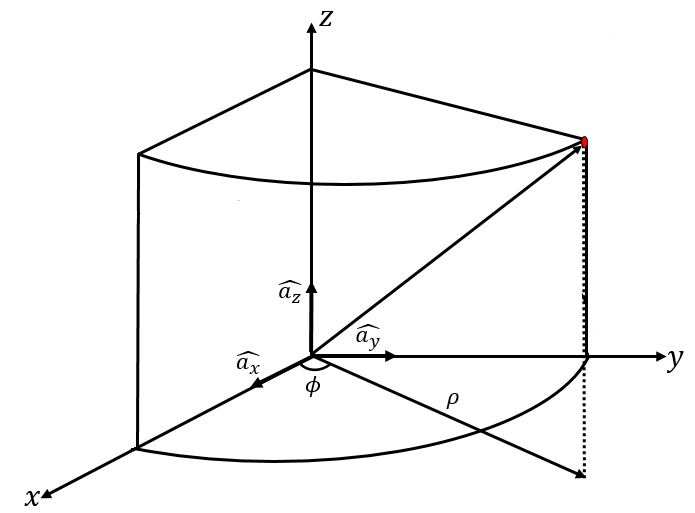
\includegraphics[width=6.09375in,height=4.49722in]{Imagenes/media/image15.png}Como
ya se mencionó, el tratamiento realizado anteriormente está bajo el
sistema de coordenadas cartesianas, ahora se va a trabajar bajo el
sistema de coordenadas cilíndricas. Considérese el siguiente sistema:

\includegraphics[width=7.17847in,height=3.73053in]{Imagenes/media/image16.emf}

\includegraphics[width=4.34615in,height=2.97151in]{Imagenes/media/image17.emf}

Se va a hacer el tratamiento para obtener una transformación del vector
posición:

\(\overrightarrow{r} = x\widehat{a_{x}} + y\widehat{a_{y}} + z\widehat{a_{z}}\)
(8)

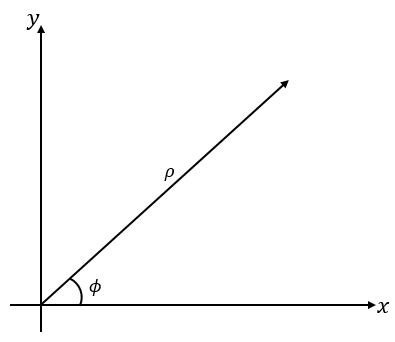
\includegraphics[width=2.64514in,height=2.42569in]{Imagenes/media/image18.png}De
la \emph{figura 6} nótese que \(\rho\) es la proyección del vector
\(\overrightarrow{r}\) en el plano \(xy\) formando un ángulo
\(\phi\ \)en el plano \(xy\) medido desde \(x\). Haciendo la
transformación de coordenadas se tiene:

Una vez obtenidas las transformaciones correspondientes se puede ver que
para este sistema existen las transformaciones inversas las cuáles están
dadas por:

\[\rho = \sqrt{x^{2} + y^{2}} = \rho(x,\ y,\ z)\]

\[\phi = \tan^{- 1}\left( \frac{y}{x} \right) = \phi(x,\ y,\ z)\]

De la ecuación (8) se procede a obtener el vector velocidad:

\(\overrightarrow{\dot{r}} = \left( \dot{\rho}\cos\phi - \rho\dot{\phi}{sen}\phi \right)\widehat{a_{x}} + \left( \dot{\rho}{sen}\phi + \rho\dot{\phi}\cos\phi \right)\widehat{a_{y}} + \dot{z}\widehat{a_{z}}\)
(10)

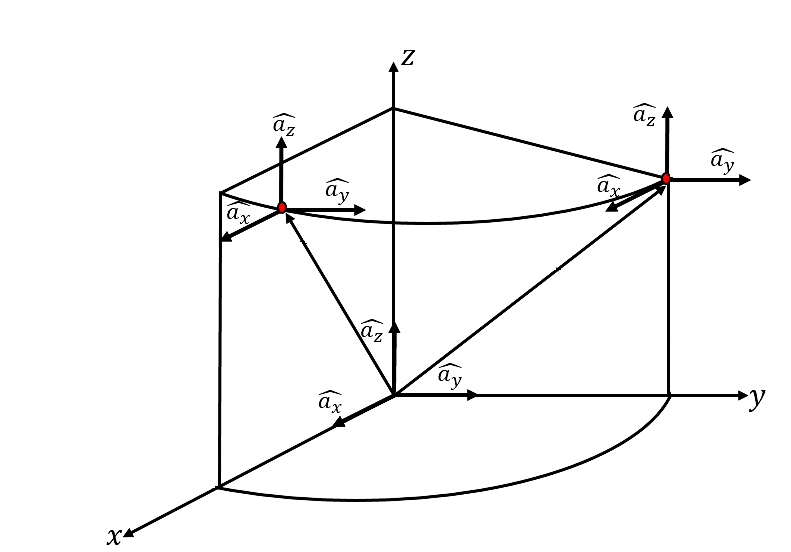
\includegraphics[width=5.70833in,height=4.26181in]{Imagenes/media/image19.png}Gráficamente:

De la ecuación (9) y de la \emph{figura 8} se puede ver que la base de
vectores
\(\left( \widehat{a_{x},}\ \widehat{a_{y},}\ \widehat{a_{z}} \right)\)
forma una base fija. Obteniendo el vector aceleración se da que:

\[\overrightarrow{\ddot{r}} = \left( \ddot{p}\cos\phi - \ddot{p}\phi{sen}\phi - \dot{p}\dot{\phi}{sen}\phi - \rho\ddot{\phi}{sen}\phi - \rho\dot{\phi^{2}}\cos\phi \right)\widehat{a_{x}}\ \ \ \ \ \ \ \ \ \ \ \ \]

\(+ \left( \ddot{p}{sen}\phi + \dot{p}\phi\cos{\phi +}\dot{p}\dot{\phi}\cos{\phi + \rho\ddot{\phi}\cos\phi} - \rho\dot{\phi^{2}}{sen}\phi \right)\widehat{a_{y}} + \ddot{z}\widehat{a_{z}}\)
(11)

\textbf{Se dificulta la interpretación física de las componentes de}
\(\overrightarrow{\dot{\mathbf{r}}}\) \textbf{y}
\(\overrightarrow{\ddot{\mathbf{r}}}\)\textbf{, esto se debe a que no se
utiliza una base propia de vectores unitarios de las coordenadas
cilíndricas.}

En este sentido se procede a obtener la base propia de vectores
unitarios de las coordenadas cilíndricas:

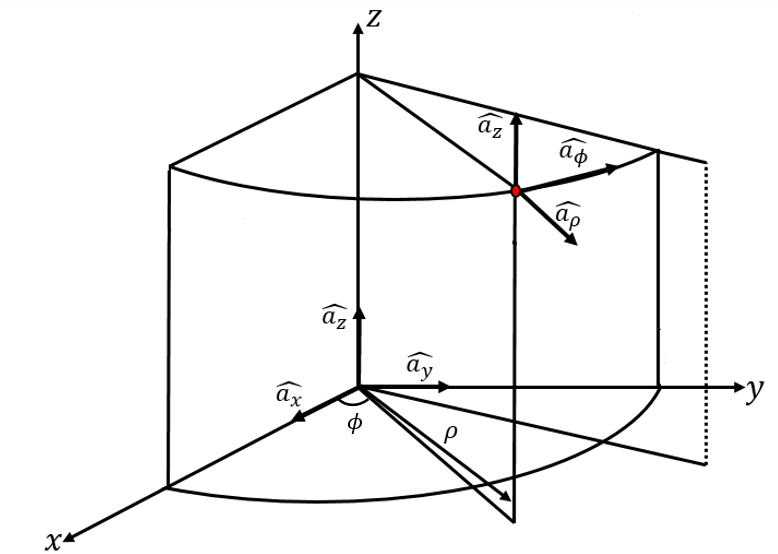
\includegraphics[width=6.30208in,height=4.45625in]{Imagenes/media/image20.png}

\[\widehat{a_{\rho}} \approx \frac{\mathrm{\Delta}\overrightarrow{r_{\rho}}}{\left| \mathrm{\Delta}\overrightarrow{r_{\rho}} \right|} = \frac{\frac{\partial\overrightarrow{r}}{\partial\rho}}{\left| \frac{\partial\overrightarrow{r}}{\partial\rho} \right|}\]

La ecuación (12) muestra el cambio del vector \(\overrightarrow{r}\) en
la dirección \(\rho\), además está normalizado.

\[\widehat{a_{\phi}} \approx \frac{\mathrm{\Delta}\overrightarrow{r_{\phi}}}{\left| \mathrm{\Delta}\overrightarrow{r_{\phi}} \right|} = \frac{\frac{\partial\overrightarrow{r}}{\partial\phi}}{\left| \frac{\partial\overrightarrow{r}}{\partial\phi} \right|}\]

La ecuación (13) muestra el cambio del vector \(\overrightarrow{r}\) en
la dirección \(\phi\), además está normalizado.

\[\widehat{a_{z}} = \widehat{a_{z}}\]

Como ya se tiene el planteamiento para la base propia de vectores
unitarios del sistema de coordenadas cilíndricas, se procede a hacer los
cálculos, de la ecuación (9) se tiene:

\[\overrightarrow{r} = \rho cos\phi\widehat{a_{x}} + \rho{sen}\phi\widehat{a_{y}} + z\widehat{a_{z}}\]

\[\frac{\partial\overrightarrow{r}}{\partial\rho} = \cos\phi\widehat{a_{x}} + {sen}\phi\widehat{a_{y}}\]

\[\left| \frac{\partial\overrightarrow{r}}{\partial\rho} \right| = \sqrt{\cos^{2}\phi + {sen}^{2}\phi} = 1\]

Por lo tanto, la ecuación (12) toma la forma:

\[\widehat{\mathbf{a}_{\mathbf{\rho}}}\mathbf{=}\mathbf{\cos}\mathbf{\phi}\widehat{\mathbf{a}_{\mathbf{x}}}\mathbf{+}\mathbf{sen}\mathbf{\phi}\widehat{\mathbf{a}_{\mathbf{y}}}\]

Análogamente, la expresión (13) queda así:

\[\widehat{\mathbf{a}_{\mathbf{\phi}}}\mathbf{= -}\mathbf{sen}\mathbf{\phi}\widehat{\mathbf{a}_{\mathbf{x}}}\mathbf{+}\mathbf{\cos}\mathbf{\phi}\widehat{\mathbf{a}_{\mathbf{y}}}\]

Además;

\[\widehat{\mathbf{a}_{\mathbf{z}}}\mathbf{=}\widehat{\mathbf{a}_{\mathbf{z}}}\]

Por lo tanto las expresiones (15), (16) y (17) corresponden a la base
\(\left( \widehat{a_{\rho},}\ \widehat{a_{\phi},}\ \widehat{a_{z}} \right)\)
propia de vectores unitarios de las coordenadas cilíndricas. Para esto
se muestra a continuación las propiedades de dicha base:

\[\widehat{a_{\rho}} \cdot \widehat{a_{\rho}} = {(cos}\phi\widehat{a_{x}} + {sen}\phi\widehat{a_{y}}) \cdot {(cos}\phi\widehat{a_{x}} + {sen}\phi\widehat{a_{y}}) = \ \cos^{2}\phi + {sen}^{2}\phi\]

\[\widehat{\mathbf{a}_{\mathbf{\rho}}}\mathbf{\cdot}\widehat{\mathbf{a}_{\mathbf{\rho}}}\mathbf{= 1}\]

\[\widehat{a_{\phi}} \cdot \widehat{a_{\phi}} = \left( - {sen}\phi\widehat{a_{x}} + \cos\phi\widehat{a_{y}} \right) \cdot \left( - {sen}\phi\widehat{a_{x}} + \cos\phi\widehat{a_{y}} \right) = {sen}^{2}\phi + \cos^{2}\phi\]

\[\widehat{\mathbf{a}_{\mathbf{\phi}}}\mathbf{\cdot}\widehat{\mathbf{a}_{\mathbf{\phi}}}\mathbf{= 1}\]

\[\widehat{a_{\rho}} \cdot \widehat{a_{\phi}} = {(cos}\phi\widehat{a_{x}} + {sen}\phi\widehat{a_{y}}) \cdot \left( - {sen}\phi\widehat{a_{x}} + \cos\phi\widehat{a_{y}} \right) = - \cos\phi{sen}{\phi +}\cos\phi{sen}\phi\]

\[\widehat{\mathbf{a}_{\mathbf{\rho}}}\mathbf{\cdot}\widehat{\mathbf{a}_{\mathbf{\phi}}}\mathbf{= 0 \rightarrow}\widehat{\mathbf{a}_{\mathbf{\rho}}}\mathbf{\bot}\widehat{\mathbf{a}_{\mathbf{\phi}}}\]

\[\widehat{a_{\rho}} \cdot \widehat{a_{z}} = {(cos}\phi\widehat{a_{x}} + {sen}\phi\widehat{a_{y}}) \cdot \widehat{a_{z}}\]

\[\widehat{\mathbf{a}_{\mathbf{\rho}}}\mathbf{\cdot}\widehat{\mathbf{a}_{\mathbf{z}}}\mathbf{= 0 \rightarrow}\widehat{\mathbf{a}_{\mathbf{\rho}}}\mathbf{\bot}\widehat{\mathbf{a}_{\mathbf{z}}}\]

Queda como ejercicio mostrar lo anterior para
\(\widehat{a_{\phi}} \cdot \widehat{a_{z}}\ \therefore\ \)

Reescribiendo ahora el vector posición con la base propia de vectores
unitarios de las coordenadas cilíndricas, se tiene:

\[\overrightarrow{r} = {\rho(cos}\phi\widehat{a_{x}} + {sen}\phi\widehat{a_{y}}) + z\widehat{a_{z}}\]

como
\({(cos}\phi\widehat{a_{x}} + {sen}\phi\widehat{a_{y}}) = \widehat{a_{p}}\)
se da que:

\[\overrightarrow{\mathbf{r}}\mathbf{= \rho}\widehat{\mathbf{a}_{\mathbf{\rho}}}\mathbf{+}\mathbf{z}\widehat{\mathbf{a}_{\mathbf{z}}}\]

La base de vectores unitarios está dada solo para mecánica traslacional,
de donde los observables toman la forma:

\[\overrightarrow{r} = x(t)\widehat{a_{x}} + y(t)\widehat{a_{y}} + z(t)\widehat{a_{z}}\]

\[\overrightarrow{\dot{r}} = \dot{x}(t)\widehat{a_{x}} + \dot{y}(t)\widehat{a_{y}} + \dot{z}(t)\widehat{a_{z}}\]

\[\overrightarrow{\ddot{r}} = \ddot{x}(t)\widehat{a_{x}} + \ddot{y}(t)\widehat{a_{y}} + \ddot{z}(t)\widehat{a_{z}}\]

\textbf{Nótese que debido a que la base es fija los vectores unitarios
no deben ser derivados. Cuando la base es móvil si es necesario conocer
la derivada de los vectores unitarios porque estos ya están variando.}

A partir del vector posición escrito para las coordenadas cilíndricas
dado en la expresión (18) se dice que la partícula ``barre'' la ``tapa''
del cilindro y se va para la superficie, de donde se obtiene el
siguiente observable:

\[\overrightarrow{\dot{r}} = \dot{\rho}\widehat{a_{\rho}} + \rho\dot{\widehat{a_{\rho}}} + \dot{z}\widehat{a_{z}}\]

\[\widehat{a_{\rho}} = \cos\phi\widehat{a_{x}} + {sen}\phi\widehat{a_{y}}\]

El vector \(\widehat{a_{z}}\) no se deriva porque \(z\) es fijo.

\[\dot{\widehat{a_{\rho}}} = \frac{d\widehat{a_{\rho}}}{dt} = - \ \dot{\phi}{sen}\phi\widehat{a_{x}} + \dot{\phi}\cos\phi\widehat{a_{y}}\]

\[\dot{\widehat{a_{\rho}}} = \dot{\phi}( - {sen}\phi\widehat{a_{x}} + \cos\phi\widehat{a_{y}})\]

\[\dot{\widehat{\mathbf{a}_{\mathbf{\rho}}}}\mathbf{=}\dot{\mathbf{\phi}}\widehat{\mathbf{a}_{\mathbf{\phi}}}\]

Luego;

\[\overrightarrow{\dot{\mathbf{r}}}\mathbf{=}\dot{\rho}\widehat{\mathbf{a}_{\mathbf{\rho}}}\mathbf{+}\rho\dot{\mathbf{\phi}}\widehat{\mathbf{a}_{\mathbf{\phi}}}\mathbf{+}\dot{\mathbf{z}}\widehat{\mathbf{a}_{\mathbf{z}}}\]

Analizando cada término de la expresión (19) se tiene que:

\(\dot{\rho}\widehat{\mathbf{a}_{\mathbf{\rho}}}\) \textbf{corresponde a
la velocidad radial.}

\(\rho\dot{\mathbf{\phi}}\widehat{\mathbf{a}_{\mathbf{\phi}}}\)
\textbf{corresponde a la velocidad angular tangencial.}

\(\mathbf{z}\widehat{\mathbf{a}_{\mathbf{z}}}\) \textbf{corresponde a la
velocidad a lo largo del eje} \(\mathbf{z}\)\textbf{.}

Ahora se procede a obtener las componentes de la aceleración:

\[\overrightarrow{\dot{\mathbf{r}}}\mathbf{=}\dot{\rho}\widehat{\mathbf{a}_{\mathbf{\rho}}}\mathbf{+}\rho\dot{\mathbf{\phi}}\widehat{\mathbf{a}_{\mathbf{\phi}}}\mathbf{+}\dot{\mathbf{z}}\widehat{\mathbf{a}_{\mathbf{z}}}\]

\[\overrightarrow{\ddot{r}} = \ddot{\rho}\widehat{a_{\rho}} + \dot{\rho}\dot{\widehat{a_{\rho}}} + \dot{\rho}\dot{\phi}\widehat{a_{\phi}} + \rho\ddot{\phi}\widehat{a_{\phi}} + \rho\dot{\phi}\dot{\widehat{a_{\phi}}} + \ddot{z}\widehat{a_{z}}\]

Donde;

\[\widehat{a_{\phi}} = - {sen}\phi\widehat{a_{x}} + \cos\phi\widehat{a_{y}}\]

\[\dot{\widehat{a_{\phi}}} = - \dot{\phi}\cos\phi\widehat{a_{x}} - \dot{\phi}{sen}\phi\widehat{a_{y}}\]

\[\dot{\widehat{a_{\phi}}} = - \dot{\phi}(\cos\phi\widehat{a_{x}} + {sen}\phi\widehat{a_{y}})\]

\[\dot{\widehat{a_{\phi}}} = - \dot{\phi}\widehat{a_{\rho}}\]

De esta manera:

\[\overrightarrow{\ddot{r}} = \ddot{\rho}\widehat{a_{\rho}} + \dot{\rho}\dot{\phi}\widehat{a_{\phi}} + \dot{\rho}\dot{\phi}\widehat{a_{\phi}} + \rho\ddot{\phi}\widehat{a_{\phi}} - \rho{\dot{\phi}}^{2}\widehat{a_{\rho}} + \ddot{z}\widehat{a_{z}}\]

\[\overrightarrow{\ddot{r}} = \ddot{\rho}\widehat{a_{\rho}} + 2\dot{\rho}\dot{\phi}\widehat{a_{\phi}} + \rho\ddot{\phi}\widehat{a_{\phi}} - \rho{\dot{\phi}}^{2}\widehat{a_{\rho}} + \ddot{z}\widehat{a_{z}}\]

Finalmente;

\[\overrightarrow{\ddot{r}} = \ddot{\rho}\widehat{a_{\rho}} + 2\dot{\rho}\dot{\phi}\widehat{a_{\phi}} + \rho\ddot{\phi}\widehat{a_{\phi}} - \rho{\dot{\phi}}^{2}\widehat{a_{p}} + \ddot{z}\widehat{a_{z}}\]

\[\overrightarrow{\ddot{\mathbf{r}}}\mathbf{=}\left( \ddot{\mathbf{\rho}}\mathbf{-}\rho{\dot{\mathbf{\phi}}}^{\mathbf{2}} \right)\widehat{\mathbf{a}_{\mathbf{\rho}}}\mathbf{+ (\rho}\ddot{\mathbf{\phi}}\mathbf{+ 2}\dot{\rho}\dot{\mathbf{\phi}}\mathbf{)}\widehat{\mathbf{a}_{\mathbf{\phi}}}\mathbf{+}\ddot{\mathbf{z}}\widehat{\mathbf{a}_{\mathbf{z}}}\]

Analizando cada término de la ecuación (20) se tiene que:

\(\ddot{\mathbf{\rho}}\widehat{\mathbf{a}_{\mathbf{\rho}}}\)
\textbf{corresponde a la aceleración radial.}

\(\mathbf{-}\rho{\dot{\mathbf{\phi}}}^{\mathbf{2}}\widehat{\mathbf{a}_{\mathbf{p}}}\)
\textbf{corresponde a la aceleración centrípeta.}

\(\mathbf{\rho}\ddot{\mathbf{\phi}}\widehat{\mathbf{a}_{\mathbf{\phi}}}\)
\textbf{corresponde a la aceleración angular.}

\(\mathbf{2}\dot{\mathbf{p}}\dot{\mathbf{\phi}}\widehat{\mathbf{a}_{\mathbf{\phi}}}\)
\textbf{corresponde a la aceleración de Coriolis.}

\(\ddot{\mathbf{z}}\widehat{\mathbf{a}_{\mathbf{z}}}\)
\textbf{corresponde a la aceleración longitudinal.}

\textbf{CINEMÁTICA EN COORDENADAS ESFÉRICAS}

Por último tómese el caso de las coordenadas esféricas. Considérese el
siguiente sistema de coordenadas:

\includegraphics[width=2.86538in,height=2.75806in]{Imagenes/media/image21.emf}\includegraphics[width=3.56946in,height=3.125in]{Imagenes/media/image22.emf}

\includegraphics[width=4.09594in,height=3.36728in]{Imagenes/media/image23.emf}

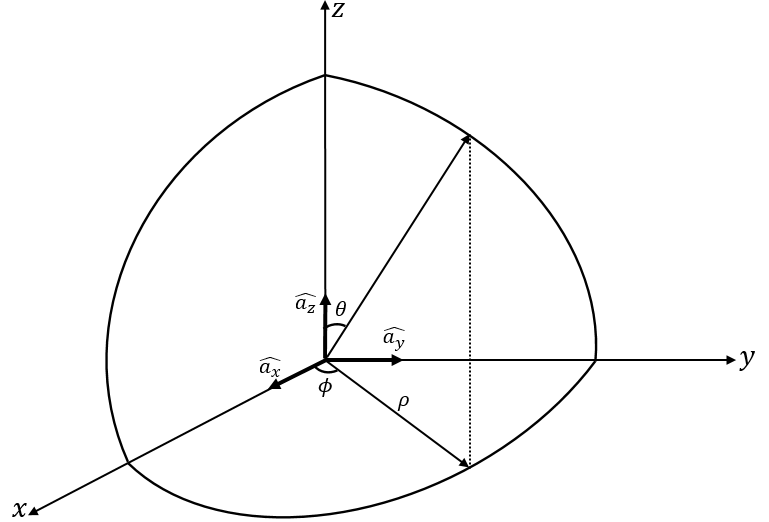
\includegraphics[width=4.46875in,height=3.10069in]{Imagenes/media/image24.png}

Tal como se realizó para el sistema de coordenadas cilíndricas, se van a
efectuar una serie de transformaciones con la finalidad de llevar el
vector posición dado en la ecuación (8) a coordenadas esféricas.

De la \emph{figura 10} se tiene que:

\[\cos\theta = \frac{z}{r} \rightarrow z = r\cos\theta\]

\[{sen}\theta = \frac{\rho}{r} \rightarrow \rho = r{sen}\theta\]

\[\cos\phi = \frac{x}{\rho} \rightarrow x = \rho\cos\phi \rightarrow x = r{sen}\theta\cos\phi\]

\[{sen}\phi = \frac{y}{\rho} \rightarrow y = \rho{sen}\phi \rightarrow y = r{sen}\theta{sen}\phi\]

Así:

\[\overrightarrow{\mathbf{r}}\mathbf{=}\mathbf{r}\mathbf{sen}\mathbf{\theta}\mathbf{\cos}\mathbf{\phi}\widehat{\mathbf{a}_{\mathbf{x}}}\mathbf{+}\mathbf{r}\mathbf{sen}\mathbf{\theta}\mathbf{sen}\mathbf{\phi}\widehat{\mathbf{a}_{\mathbf{y}}}\mathbf{+ r}\mathbf{\cos}\mathbf{\theta}\widehat{\mathbf{a}_{\mathbf{z}}}\]

Ejercicio: Obtener \(\overrightarrow{\dot{r}}\) y
\(\overrightarrow{\ddot{r}}\ \ \therefore\)

A continuación se va a hallar la base propia de vectores unitarios
asociada a las coordenadas esféricas:

\[\widehat{a_{r}} \approx \frac{\mathrm{\Delta}\overrightarrow{r_{r}}}{\left| \mathrm{\Delta}\overrightarrow{r_{r}} \right|} = \frac{\frac{\partial\overrightarrow{r}}{\partial r}}{\left| \frac{\partial\overrightarrow{r}}{\partial r} \right|}\]

La ecuación (22) muestra el cambio del vector \(\overrightarrow{r}\) en
la dirección \(r\), además está normalizado.

\[\widehat{a_{\phi}} \approx \frac{\mathrm{\Delta}\overrightarrow{r_{\phi}}}{\left| \mathrm{\Delta}\overrightarrow{r_{\phi}} \right|} = \frac{\frac{\partial\overrightarrow{r}}{\partial\phi}}{\left| \frac{\partial\overrightarrow{r}}{\partial\phi} \right|}\]

La ecuación (23) muestra el cambio del vector \(\overrightarrow{r}\) en
la dirección \(\phi\) y está normalizado.

\[\widehat{a_{\theta}} \approx \frac{\mathrm{\Delta}\overrightarrow{r_{\theta}}}{\left| \mathrm{\Delta}\overrightarrow{r_{\theta}} \right|} = \frac{\frac{\partial\overrightarrow{r}}{\partial\theta}}{\left| \frac{\partial\overrightarrow{r}}{\partial\theta} \right|}\]

La ecuación (24) muestra el cambio del vector \(\overrightarrow{r}\) en
la dirección \(\theta\), además está normalizado.

Una vez tenido el planteamiento para la base propia de vectores
unitarios del sistema de coordenadas esféricas, solo queda hacer los
cálculos, de la ecuación (21):

\[\overrightarrow{\mathbf{r}}\mathbf{=}\mathbf{r}\mathbf{sen}\mathbf{\theta}\mathbf{\cos}\mathbf{\phi}\widehat{\mathbf{a}_{\mathbf{x}}}\mathbf{+}\mathbf{r}\mathbf{sen}\mathbf{\theta}\mathbf{sen}\mathbf{\phi}\widehat{\mathbf{a}_{\mathbf{y}}}\mathbf{+ r}\mathbf{\cos}\mathbf{\theta}\widehat{\mathbf{a}_{\mathbf{z}}}\]

\[\frac{\partial\overrightarrow{r}}{\partial r} = {sen}\theta\cos\phi\widehat{a_{x}} + {sen}\theta{sen}\phi\widehat{a_{y}} + \cos\theta\widehat{a_{z}}\]

\[\left| \frac{\partial\overrightarrow{r}}{\partial r} \right| = \sqrt{{sen}^{2}\theta\cos^{2}\phi + {sen}^{2}\theta{sen}^{2}\phi + \cos^{2}\theta} = 1\]

De esta manera la ecuación (22) toma la forma:

\(\widehat{\mathbf{a}_{\mathbf{r}}}\mathbf{=}\mathbf{sen}\mathbf{\theta}\mathbf{\cos}\mathbf{\phi}\widehat{\mathbf{a}_{\mathbf{x}}}\mathbf{+}\mathbf{sen}\mathbf{\theta}\mathbf{sen}\mathbf{\phi}\widehat{\mathbf{a}_{\mathbf{y}}}\mathbf{+}\mathbf{\cos}\mathbf{\theta}\widehat{\mathbf{a}_{\mathbf{z}}}\)
(25)

Análogamente las ecuaciones (23) y (24) toman respectivamente la forma:

\(\widehat{\mathbf{a}_{\mathbf{\phi}}}\mathbf{= -}\mathbf{sen}\mathbf{\phi}\widehat{\mathbf{a}_{\mathbf{x}}}\mathbf{+}\mathbf{\cos}\mathbf{\phi}\widehat{\mathbf{a}_{\mathbf{y}}}\)
(26)

\(\widehat{\mathbf{a}_{\mathbf{\theta}}}\mathbf{=}\mathbf{\cos}\mathbf{\theta}\mathbf{\cos}\mathbf{\phi}\widehat{\mathbf{a}_{\mathbf{x}}}\mathbf{+}\mathbf{\cos}\mathbf{\theta}\mathbf{sen}\mathbf{\phi}\widehat{\mathbf{a}_{\mathbf{y}}}\mathbf{-}\mathbf{sen}\mathbf{\theta}\widehat{\mathbf{a}_{\mathbf{z}}}\)
(27)

Las ecuaciones (25), (26) y (27) corresponden a la base
\(\left( \widehat{a_{r},}\ \widehat{a_{\phi},}\ \widehat{a_{\theta}} \right)\)
propia de vectores unitarios de las coordenadas esféricas. De esta
manera se hace necesario probar que dicha base si corresponde a una base
de vectores unitarios, por lo tanto:

\(\widehat{a_{r}} \cdot \widehat{a_{r}} = {sen}^{2}\theta\cos^{2}\phi + {sen}^{2}\theta{sen}^{2}\phi + \cos^{2}\theta\)\(= {sen}^{2}\theta\left( \cos^{2}\phi + {sen}^{2}\phi \right) + \cos^{2}\theta\)

\(\widehat{\mathbf{a}_{\mathbf{r}}}\mathbf{\cdot}\widehat{\mathbf{a}_{\mathbf{r}}}\mathbf{= 1}\)

\textbf{\hfill\break
}

\[\widehat{a_{\theta}} \cdot \widehat{a_{\theta}} = \cos^{2}\theta\cos^{2}\phi + \cos^{2}\theta{sen}^{2}\phi + {sen}^{2}\theta = \cos^{2}\theta\left( \cos^{2}\phi + {sen}^{2}\phi \right) + {sen}^{2}\theta\]

\[\widehat{\mathbf{a}_{\mathbf{\theta}}}\mathbf{\cdot}\widehat{\mathbf{a}_{\mathbf{\theta}}}\mathbf{= 1}\]

\[\widehat{a_{\phi}} \cdot \widehat{a_{\phi}} = \left( - {sen}\phi\widehat{a_{x}} + \cos\phi\widehat{a_{y}} \right) \cdot ( - {sen}\phi\widehat{a_{x}} + \cos\phi\widehat{a_{y}})\]

\[\widehat{a_{\phi}} \cdot \widehat{a_{\phi}} = {sen}^{2}\phi + \cos^{2}\phi\]

\[\widehat{\mathbf{a}_{\mathbf{\phi}}}\mathbf{\cdot}\widehat{\mathbf{a}_{\mathbf{\phi}}}\mathbf{= 1}\]

\[\widehat{a_{r}} \cdot \widehat{a_{\theta}} = {sen}\theta\cos\theta\cos^{2}\phi + {sen}\theta\cos\theta{sen}^{2}\phi - {sen}\theta\cos\theta\]

\[\widehat{a_{r}} \cdot \widehat{a_{\theta}} = {sen}\theta\cos\theta(\cos^{2}\phi + {sen}^{2}\phi) - {sen}\theta\cos\theta\]

\[\widehat{\mathbf{a}_{\mathbf{r}}}\mathbf{\cdot}\widehat{\mathbf{a}_{\mathbf{\theta}}}\mathbf{= 0 \rightarrow}\widehat{\mathbf{a}_{\mathbf{r}}}\mathbf{\bot}\widehat{\mathbf{a}_{\mathbf{\theta}}}\]

\[\widehat{a_{r}} \cdot \widehat{a_{\phi}} = \left( {sen}\theta\cos\phi\widehat{a_{x}} + {sen}\theta{sen}\phi\widehat{a_{y}} + \cos\theta\widehat{a_{z}} \right) \cdot ( - {sen}\phi\widehat{a_{x}} + \cos\phi\widehat{a_{y}})\]

\[\widehat{a_{r}} \cdot \widehat{a_{\phi}} = - {sen}\theta\cos\phi{sen}\phi + {sen}\theta{sen}\phi\cos\phi\]

\[\widehat{\mathbf{a}_{\mathbf{r}}}\mathbf{\cdot}\widehat{\mathbf{a}_{\mathbf{\phi}}}\mathbf{= 0 \rightarrow}\widehat{\mathbf{a}_{\mathbf{r}}}\mathbf{\bot}\widehat{\mathbf{a}_{\mathbf{\phi}}}\]

Queda como ejercicio realizar lo anterior para
\(\widehat{a_{\theta}} \cdot \widehat{a_{\phi}}\ \therefore\)

Del desarrollo realizado anteriormente se puede concluir que la base
ortonormal propia de las coordenadas esféricas es completamente móvil,
por lo que de acuerdo al \emph{delta de Kronecker} se da que:

\[\widehat{a_{i}} \bullet \widehat{a_{j}} = \delta_{ij}\]

Ahora se va a encontrar la velocidad y la aceleración en el sistema de
coordenadas esféricas en términos de la base propia de vectores
unitarios. Para esto se parte de la ecuación (21) de donde se tiene que:

\[\overrightarrow{r} = r({sen}\theta\cos\phi\widehat{a_{x}} + {sen}\theta{sen}\phi\widehat{a_{y}} + \cos\theta\widehat{a_{z}})\]

Como
\(r\left( {sen}\theta\cos\phi\widehat{a_{x}} + {sen}\theta{sen}\phi\widehat{a_{y}} + \cos\theta\widehat{a_{z}} \right) = \widehat{a_{r}}\)
entonces:

\(\overrightarrow{\mathbf{r}}\mathbf{=}\mathbf{r}\widehat{\mathbf{a}_{\mathbf{r}}}\)
(28)

Para las componentes de la velocidad, a partir de la ecuación (28) se da
que:

\[\overrightarrow{\dot{r}} = \dot{r}\widehat{a_{r}} + r\dot{\widehat{a_{r}}}\]

Como

\[\dot{\widehat{a_{r}}} = \left( \dot{\theta}\cos\theta\cos\phi - \dot{\phi}{sen}{\theta{sen}\phi} \right)\widehat{a_{x}} + \left( \dot{\theta}\cos\theta{sen}\phi + \dot{\phi}{sen}{\theta\cos\phi} \right)\widehat{a_{y}} - \dot{\theta}{sen}\theta\widehat{a_{z}}\]

\(\dot{\widehat{a_{r}}} = \dot{\theta}\left( \cos\theta\cos\phi\widehat{a_{x}} + \cos\theta{sen}\phi\widehat{a_{y}} - {sen}\theta\widehat{a_{z}} \right) + \dot{\phi}{sen}\theta( - {sen}\phi\widehat{a_{x}} + \cos\phi\widehat{a_{y}}\))

Además
\(\cos\theta\cos\phi\widehat{a_{x}} + \cos\theta{sen}\phi\widehat{a_{y}} - {sen}\theta\widehat{a_{z}} = \widehat{a_{\theta}}\)
y
\(- {sen}\phi\widehat{a_{x}} + \cos\phi\widehat{a_{y}} = \widehat{a_{\phi}}\)
entonces:

\[\dot{\widehat{a_{r}}} = \dot{\mathbf{\theta}}\widehat{\mathbf{a}_{\mathbf{\theta}}}\mathbf{+}\mathbf{sen}\mathbf{\theta}\dot{\mathbf{\phi}}\widehat{\mathbf{a}_{\mathbf{\phi}}}\]

\(\overrightarrow{\dot{\mathbf{r}}}\mathbf{=}\dot{\mathbf{r}}\widehat{\mathbf{a}_{\mathbf{r}}}\mathbf{+ r}\dot{\mathbf{\theta}}\widehat{\mathbf{a}_{\mathbf{\theta}}}\mathbf{+ r}\mathbf{sen}\mathbf{\theta}\dot{\mathbf{\phi}}\widehat{\mathbf{a}_{\mathbf{\phi}}}\)
(29)

De la expresión (29) se puede tener una interpretación para cada
término, de este modo:

\(\dot{\mathbf{r}}\widehat{\mathbf{a}_{\mathbf{r}}}\)
\textbf{corresponde la velocidad radial.}

\(\mathbf{r}\dot{\mathbf{\theta}}\widehat{\mathbf{a}_{\mathbf{\theta}}}\)
\textbf{corresponde a la velocidad angular.}

\(\mathbf{r}\mathbf{sen}\mathbf{\theta}\dot{\mathbf{\phi}}\widehat{\mathbf{a}_{\mathbf{\phi}}}\)
\textbf{corresponde a la velocidad azimutal.}

Así mismo, de la ecuación (29) se tiene para la aceleración que:

Obteniendo los vectores unitarios de la base propia de las coordenadas
esféricas para la aceleración, se tiene:

\(\widehat{\mathbf{a}_{\mathbf{\theta}}}\mathbf{=}\mathbf{\cos}\mathbf{\theta}\mathbf{\cos}\mathbf{\phi}\widehat{\mathbf{a}_{\mathbf{x}}}\mathbf{+}\mathbf{\cos}\mathbf{\theta}\mathbf{sen}\mathbf{\phi}\widehat{\mathbf{a}_{\mathbf{y}}}\mathbf{-}\mathbf{sen}\mathbf{\theta}\widehat{\mathbf{a}_{\mathbf{z}}}\)

Como
\({sen}{\theta\cos\phi\widehat{a_{x}}} + {sen}{\theta{sen}\phi}\widehat{a_{y}} + \cos\theta\widehat{a_{z}} = \widehat{a_{r}}\)
y
\(- {sen}\phi\widehat{a_{x}} + \cos{\phi\widehat{a_{y}}} = \widehat{a_{\phi}}\):

\[\dot{\widehat{a_{\theta}}}\mathbf{= -}\dot{\mathbf{\theta}}\widehat{\mathbf{a}_{\mathbf{r}}}\mathbf{+}\dot{\mathbf{\phi}}\mathbf{\cos}\mathbf{\theta}\widehat{\mathbf{a}_{\mathbf{\phi}}}\]

\[\dot{\widehat{a_{r}}} = \dot{\mathbf{\theta}}\widehat{\mathbf{a}_{\mathbf{\theta}}}\mathbf{+}\mathbf{sen}\mathbf{\theta}\dot{\mathbf{\phi}}\widehat{\mathbf{a}_{\mathbf{\phi}}}\]

Para \(\dot{\widehat{a_{\phi}}}\) se tiene:

\[\dot{\widehat{a_{\phi}}} = - \dot{\phi}\cos\phi\widehat{a_{x}} - \dot{\phi}{sen}\phi\widehat{a_{y}}\]

\[\dot{\widehat{a_{\phi}}} = - \dot{\phi}(\cos\phi\widehat{a_{x}} + {sen}\phi\widehat{a_{y}})\]

Como
\(\cos\phi\widehat{a_{x}} + {sen}\phi\widehat{a_{y}} = {sen}\theta\widehat{a_{r}} + \cos\theta\widehat{a_{\theta}}\)
entonces:

\[\dot{\widehat{a_{\phi}}} = - \dot{\phi}({sen}\theta\widehat{a_{r}} + \cos\theta\widehat{a_{\theta}})\]

Por otro lado se da que:

\[{sen}\theta\widehat{a_{r}} = {sen}\theta({sen}\theta\cos\phi\widehat{a_{x}} + {sen}\theta{sen}\phi\widehat{a_{y}} + \cos\theta\widehat{a_{z}})\]

\[\cos\theta\widehat{a_{\theta}} = \cos\theta(\cos\theta\cos\phi\widehat{a_{x}} + \cos\theta{sen}\phi\widehat{a_{y}} - {sen}\theta\widehat{a_{z}})\]

De este modo:

\[{sen}\theta\widehat{a_{r}} + \cos\theta\widehat{a_{\theta}} = \cos\phi\widehat{a_{x}} + {sen}\phi\widehat{a_{y}}\]

Por lo tanto:

\[\dot{\widehat{\mathbf{a}_{\mathbf{\phi}}}}\mathbf{= -}\dot{\mathbf{\phi}}\mathbf{sen}\mathbf{\theta}\widehat{\mathbf{a}_{\mathbf{r}}}\mathbf{-}\dot{\mathbf{\phi}}\mathbf{\cos}\mathbf{\theta}\widehat{\mathbf{a}_{\mathbf{\theta}}}\]

\[\overrightarrow{\ddot{r}} = \ddot{r}\widehat{a_{r}} + \dot{r}\dot{\widehat{a_{r}}} + \dot{r}\dot{\theta}\widehat{a_{\theta}} + r\ddot{\theta}\widehat{a_{\theta}} + r\dot{\theta}\dot{\widehat{a_{\theta}}} + \dot{r}{sen}{\theta\dot{\phi}}\widehat{a_{\phi}} + r\cos{\theta\dot{\phi}}\dot{\theta}\widehat{a_{\phi}} + r{sen}\theta\ddot{\phi}\widehat{a_{\phi}} + r{sen}{\theta\dot{\phi}\dot{\widehat{a_{\phi}}}}\]

De esta manera la aceleración en coordenadas esféricas es:

\[\overrightarrow{\ddot{r}} = \ddot{r}\widehat{a_{r}} + \dot{r}\dot{\theta}\widehat{a_{\theta}} + \dot{r}\dot{\phi}{sen}\theta\widehat{a_{\phi}} + \dot{r}\dot{\theta}\widehat{a_{\theta}} + r\ddot{\theta}\widehat{a_{\theta}} - r{\dot{\theta}}^{2}\widehat{a_{r}} + r\dot{\theta}\dot{\phi}\cos\theta\widehat{a_{\phi}} + \dot{r}{sen}\theta\dot{\phi}\widehat{a_{\phi}}\]

\[\overrightarrow{\ddot{\mathbf{r}}}\mathbf{=}\left( \ddot{\mathbf{r}}\mathbf{- r}{\dot{\mathbf{\theta}}}^{\mathbf{2}}\mathbf{- r}\mathbf{sen}^{\mathbf{2}}\mathbf{\theta}{\dot{\mathbf{\phi}}}^{\mathbf{2}} \right)\widehat{\mathbf{a}_{\mathbf{r}}}\mathbf{+}\left( \mathbf{r}\ddot{\mathbf{\theta}}\mathbf{+ 2}\dot{\mathbf{r}}\dot{\mathbf{\theta}}\mathbf{- r}\mathbf{sen}\mathbf{\theta}\mathbf{\cos}\mathbf{\theta}{\dot{\mathbf{\phi}}}^{\mathbf{2}} \right)\widehat{\mathbf{a}_{\mathbf{\theta}}}\]

Ejercicio: Mostrar que \(\therefore\ \)

\[\widehat{a_{x}} \times \widehat{a_{y}} = \widehat{a_{z}}\ \ \ \ \ \ \ \ \ \ \ \ \ \ \ \ \ \ \ \ \ \widehat{a_{y}} \times \widehat{a_{z}} = \widehat{a_{x}}\ \ \ \ \ \ \ \ \ \ \ \ \ \ \ \ \ \ \ \ \ \widehat{a_{z}} \times \widehat{a_{x}} = \widehat{a_{y}}\]

\[\widehat{a_{p}} \times \widehat{a_{\phi}} = \widehat{a_{z}}\ \ \ \ \ \ \ \ \ \ \ \ \ \ \ \ \ \ \ \ \ \widehat{a_{\phi}} \times \widehat{a_{z}} = \widehat{a_{\rho}}\ \ \ \ \ \ \ \ \ \ \ \ \ \ \ \ \ \ \ \ \ \widehat{a_{z}} \times \widehat{a_{\rho}} = \widehat{a_{\phi}}\]

\[\widehat{a_{r}} \times \widehat{a_{\theta}} = \widehat{a_{\phi}}\ \ \ \ \ \ \ \ \ \ \ \ \ \ \ \ \ \ \ \ \ \widehat{a_{\theta}} \times \widehat{a_{\phi}} = \widehat{a_{r}}\ \ \ \ \ \ \ \ \ \ \ \ \ \ \ \ \ \ \ \ \ \widehat{a_{\phi}} \times \widehat{a_{r}} = \widehat{a_{\theta}}\]

\textbf{CINEMÁTICA EN COORDENADAS CURVILÍNEAS}

Luego de haber hecho todo el tratamiento en los distintos sistemas de
coordenadas se puede ver que cada uno tiene la definición para los
observables físicos de una manera muy particular por lo que se hace
necesario tener un sistema de coordenadas curvilíneas que no
particularicen tanto dichos observables, es por esto que a continuación
se van a obtener las coordenadas generalizadas y las distintas
magnitudes físicas.

Sean \(S_{1}\), \(S_{2}\) y \(S_{3}\) tres superficies con simetría
arbitraria, sean \(q_{1}\), \(q_{2}\) y \(q_{3}\) tres curvas dadas por
la intersección de dos de las tres superficies según corresponda; y sea
\(P\) un punto definido por la intersección de las tres superficies tal
como se muestra en la \emph{figura 11.}

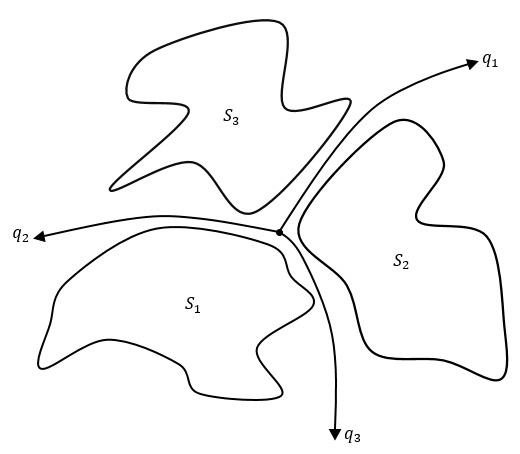
\includegraphics[width=5.15625in,height=4.46111in]{Imagenes/media/image25.jpeg}

En coordenadas generalizadas el vector posición va a estar dado por:

\(\overrightarrow{r}\left( q_{1},\ q_{2},\ q_{3};\ t \right) = x\left( q_{1},\ q_{2},\ q_{3};\ t \right)\widehat{a_{x}} + y\left( q_{1},\ q_{2},\ q_{3};\ t \right)\widehat{a_{y}} + z\left( q_{1},\ q_{2},\ q_{3};\ t \right)\widehat{a_{z}}\)
(33)

Nótese que este vector está escrito en términos de una base que NO es
propia de las coordenadas generalizadas, por lo que se hace necesario
encontrar la base propia de las coordenadas generalizadas de vectores NO
unitarios, de esta manera:

\[\widehat{a_{1}} = \frac{\frac{\partial\overrightarrow{r}}{\partial q_{1}}}{\left| \frac{\partial\overrightarrow{r}}{\partial q_{1}} \right|} \rightarrow \frac{\partial\overrightarrow{r}}{\partial q_{1}} = \left| \frac{\partial\overrightarrow{r}}{\partial q_{1}} \right|\widehat{a_{1}}\]

La ecuación (34) muestra el cambio del vector \(\overrightarrow{r}\) en
la dirección \(q_{1}\) y está normalizado.

\[\widehat{a_{2}} = \frac{\frac{\partial\overrightarrow{r}}{\partial q_{2}}}{\left| \frac{\partial\overrightarrow{r}}{\partial q_{2}} \right|} \rightarrow \frac{\partial\overrightarrow{r}}{\partial q_{2}} = \left| \frac{\partial\overrightarrow{r}}{\partial q_{2}} \right|\widehat{a_{2}}\]

La ecuación (35) muestra el cambio del vector \(\overrightarrow{r}\) en
la dirección \(q_{2}\) y está normalizado.

\[\widehat{a_{3}} = \frac{\frac{\partial\overrightarrow{r}}{\partial q_{3}}}{\left| \frac{\partial\overrightarrow{r}}{\partial q_{3}} \right|} \rightarrow \frac{\partial\overrightarrow{r}}{\partial q_{3}} = \left| \frac{\partial\overrightarrow{r}}{\partial q_{3}} \right|\widehat{a_{3}}\]

La ecuación (36) muestra el cambio del vector \(\overrightarrow{r}\) en
la dirección \(q_{3}\) y está normalizado.

Los vectores escritos en las ecuaciones (34), (35) y (36) son vectores
NO unitarios y en general NO forman una base ortonormal. Ahora se
procede a obtener los cambios que van a tomar las curvas cuando se
intersectan las superficies, así:

\[\frac{\partial\overrightarrow{r}}{\partial q_{1}} = \frac{\partial x\left( q_{1},\ q_{2},\ q_{3};\ t \right)}{\partial q_{1}}\widehat{a_{x}} + \frac{\partial y\left( q_{1},\ q_{2},\ q_{3};\ t \right)}{\partial q_{1}}\widehat{a_{y}} + \frac{\partial z\left( q_{1},\ q_{2},\ q_{3};\ t \right)}{\partial q_{1}}\widehat{a_{z}} = \overrightarrow{b_{1}}\]

La expresión (37) muestra el cambio que toma la curva \(q_{1}\ \)cuando
se intersectan las superficies \(S_{2}\) y \(S_{3}\).

\[\frac{\partial\overrightarrow{r}}{\partial q_{2}} = \frac{\partial x\left( q_{1},\ q_{2},\ q_{3};\ t \right)}{\partial q_{2}}\widehat{a_{x}} + \frac{\partial y\left( q_{1},\ q_{2},\ q_{3};\ t \right)}{\partial q_{2}}\widehat{a_{y}} + \frac{\partial z\left( q_{1},\ q_{2},\ q_{3};\ t \right)}{\partial q_{2}}\widehat{a_{z}} = \overrightarrow{b_{2}}\]

La expresión (38) muestra el cambio que toma la curva \(q_{2}\ \)cuando
se intersectan las superficies \(S_{1}\) y \(S_{3}\).

\[\frac{\partial\overrightarrow{r}}{\partial q_{3}} = \frac{\partial x\left( q_{1},\ q_{2},\ q_{3};\ t \right)}{\partial q_{3}}\widehat{a_{x}} + \frac{\partial y\left( q_{1},\ q_{2},\ q_{3};\ t \right)}{\partial q_{3}}\widehat{a_{y}} + \frac{\partial z\left( q_{1},\ q_{2},\ q_{3};\ t \right)}{\partial q_{3}}\widehat{a_{z}} = \overrightarrow{b_{3}}\]

La expresión (39) muestra el cambio que toma la curva \(q_{3}\ \)cuando
se intersectan las superficies \(S_{1}\) y \(S_{2}\).

Así mismo se define la norma de estos vectores de la siguiente manera:

\[\left| \frac{\partial\overrightarrow{r}}{\partial q_{1}} \right| = \sqrt{\left( \frac{\partial x}{\partial q_{1}} \right)^{2} + \left( \frac{\partial y}{\partial q_{1}} \right)^{2} + \left( \frac{\partial z}{\partial q_{1}} \right)^{2}} = h_{1}\]

\[\left| \frac{\partial\overrightarrow{r}}{\partial q_{2}} \right| = \sqrt{\left( \frac{\partial x}{\partial q_{2}} \right)^{2} + \left( \frac{\partial y}{\partial q_{2}} \right)^{2} + \left( \frac{\partial z}{\partial q_{2}} \right)^{2}} = h_{2}\]

\[\left| \frac{\partial\overrightarrow{r}}{\partial q_{3}} \right| = \sqrt{\left( \frac{\partial x}{\partial q_{3}} \right)^{2} + \left( \frac{\partial y}{\partial q_{3}} \right)^{2} + \left( \frac{\partial z}{\partial q_{3}} \right)^{2}} = h_{3}\]

Por lo tanto:

\[\overrightarrow{b_{1}} = h_{1}\widehat{a_{1}}\]

\[\overrightarrow{b_{2}} = h_{2}\widehat{a_{2}}\]

\[\overrightarrow{b_{3}} = h_{3}\widehat{a_{3}}\]

\includegraphics[width=5.34615in,height=3.55672in]{Imagenes/media/image26.emf}

\(\overrightarrow{b_{1}}\), \(\overrightarrow{b_{2}}\) y
\(\overrightarrow{b_{3}}\) forman una base de vectores unitarios no
coplanar y existe si y sólo si existe una base recíproca dada por:

\[\overrightarrow{B_{1}} = \frac{1}{h_{1}}\widehat{a_{1}}\]

\[\overrightarrow{B_{2}} = \frac{1}{h_{2}}\widehat{a_{2}}\]

\[\overrightarrow{B_{3}} = \frac{1}{h_{3}}\widehat{a_{3}}\]

Reescribiendo \(\overrightarrow{b_{1}}\), \(\overrightarrow{b_{2}}\) y
\(\overrightarrow{b_{3}}\):

\[\overrightarrow{b_{1}} = b_{1}x\widehat{a_{x}} + b_{1}y\widehat{a_{y}} + b_{1}z\widehat{a_{z}}\]

\[\overrightarrow{b_{2}} = b_{2}x\widehat{a_{x}} + b_{2}y\widehat{a_{y}} + b_{2}z\widehat{a_{z}}\]

\[\overrightarrow{b_{3}} = b_{3}x\widehat{a_{x}} + b_{3}y\widehat{a_{y}} + b_{3}z\widehat{a_{z}}\]

La combinación lineal de los vectores \(\overrightarrow{b_{1}}\),
\(\overrightarrow{b_{2}}\) y \(\overrightarrow{b_{3}}\) forman otro
vector en el espacio que se puede escribir como:

\[\overrightarrow{A} = \alpha_{1}\overrightarrow{b_{1}} + \alpha_{2}\overrightarrow{b_{2}} + \alpha_{3}\overrightarrow{b_{3}}\]

\[\overrightarrow{A} = A_{x}\widehat{a_{x}} + A_{y}\widehat{a_{y}} + A_{z}\widehat{a_{z}}\]

\[A_{x} = \alpha_{1}b_{1}x + \alpha_{2}b_{2}x + \alpha_{3}b_{3}x\]

\[A_{y} = \alpha_{1}b_{1}y + \alpha_{2}b_{2}y + \alpha_{3}b_{3}y\]

\[A_{z} = \alpha_{1}b_{1}z + \alpha_{2}b_{2}z + \alpha_{3}b_{3}z\]

Calculando \(\alpha_{1}\),\(\ \alpha_{2}\) y \(\alpha_{3}\); se tiene:

\[\alpha_{1} = \frac{\left| \begin{matrix}
A_{x} & A_{y} & A_{z} \\
b_{2}x & b_{2}y & b_{2}z \\
b_{3}x & b_{3}y & b_{3}z \\
\end{matrix} \right|}{\left| \begin{matrix}
b_{1}x & b_{1}y & b_{1}z \\
b_{2}x & b_{2}y & b_{2}z \\
b_{3}x & b_{3}y & b_{3}z \\
\end{matrix} \right|} = \frac{\overrightarrow{A} \cdot \left( \overrightarrow{b_{2}} \times \overrightarrow{b_{3}} \right)}{\overrightarrow{b_{1}} \cdot \left( \overrightarrow{b_{2}} \times \overrightarrow{b_{3}} \right)}\]

\[\alpha_{2} = \frac{\left| \begin{matrix}
A_{x} & A_{y} & A_{z} \\
b_{3}x & b_{3}y & b_{3}z \\
b_{1}x & b_{1}y & b_{1}z \\
\end{matrix} \right|}{\left| \begin{matrix}
b_{1}x & b_{1}y & b_{1}z \\
b_{2}x & b_{2}y & b_{2}z \\
b_{3}x & b_{3}y & b_{3}z \\
\end{matrix} \right|} = \frac{\overrightarrow{A} \cdot \left( \overrightarrow{b_{3}} \times \overrightarrow{b_{1}} \right)}{\overrightarrow{b_{1}} \cdot \left( \overrightarrow{b_{2}} \times \overrightarrow{b_{3}} \right)}\]

\[\alpha_{3} = \frac{\left| \begin{matrix}
A_{x} & A_{y} & A_{z} \\
b_{1}x & b_{1}y & b_{1}z \\
b_{2}x & b_{2}y & b_{2}z \\
\end{matrix} \right|}{\left| \begin{matrix}
b_{1}x & b_{1}y & b_{1}z \\
b_{2}x & b_{2}y & b_{2}z \\
b_{3}x & b_{3}y & b_{3}z \\
\end{matrix} \right|} = \frac{\overrightarrow{A} \cdot \left( \overrightarrow{b_{1}} \times \overrightarrow{b_{2}} \right)}{\overrightarrow{b_{1}} \cdot \left( \overrightarrow{b_{2}} \times \overrightarrow{b_{3}} \right)}\]

\(\overrightarrow{b_{1}} \cdot \left( \overrightarrow{b_{2}} \times \overrightarrow{b_{3}} \right)\)
es no coplanar. Cada coordenada puede escribirse en términos de las
nuevas coordenadas generalizadas y viceversa, esto es:

\[x = x\left( q_{1},\ q_{2},\ q_{3} \right)\ \ \ \ \ \ \ \ \ \ \ y = y\left( q_{1},\ q_{2},\ q_{3} \right)\ \ \ \ \ \ \ \ \ \ \ z = z\left( q_{1},\ q_{2},\ q_{3} \right)\]

\[q_{1} = q_{1}(x,\ y,\ z)\ \ \ \ \ \ \ \ \ \ \ \ q_{2} = q_{2}(x,\ y,\ z)\ \ \ \ \ \ \ \ \ \ \ \ {\ q}_{3} = q_{3}(x,\ y,\ z)\ \]

Además:

\[\overrightarrow{b_{1}} \cdot \left( \overrightarrow{b_{2}} \times \overrightarrow{b_{3}} \right) = \left| \begin{matrix}
b_{1}x & b_{1}y & b_{1}z \\
b_{2}x & b_{2}y & b_{2}z \\
b_{3}x & b_{3}y & b_{3}z \\
\end{matrix} \right| = \left| \begin{matrix}
\frac{\partial x}{\partial q_{1}} & \frac{\partial y}{\partial q_{1}} & \frac{\partial z}{\partial q_{1}} \\
\frac{\partial x}{\partial q_{2}} & \frac{\partial y}{\partial q_{2}} & \frac{\partial z}{\partial q_{3}} \\
\frac{\partial x}{\partial q_{3}} & \frac{\partial y}{\partial q_{3}} & \frac{\partial z}{\partial q_{3}} \\
\end{matrix} \right| \neq 0\]

Nótese que el determinante escrito en (40) corresponde al
\emph{Jacobiano} que es diferente de cero, esto implica que se puede
tener una transformación inversa de coordenadas.

\[\frac{\partial(x,\ y,\ z)}{\partial(q_{1},q_{2},q_{3})} \neq 0\]

\includegraphics[width=3.99028in,height=2.74028in]{Imagenes/media/image27.emf}

\(\overrightarrow{B_{1}}\), \(\overrightarrow{B_{2}}\ \)y
\(\overrightarrow{B_{3}}\ \)es la base recíproca y es la que da las
fuerzas de ligadura.

\(\overrightarrow{B_{1}}\) es un vector perpendicular al plano formado
por \(\overrightarrow{b_{2}}\) y \(\overrightarrow{b_{3}}\).

\(\overrightarrow{B_{2}}\) es un vector perpendicular al plano formado
por \(\overrightarrow{b_{1}}\) y \(\overrightarrow{b_{3}}\).

\(\overrightarrow{B_{3}}\) es un vector perpendicular al plano formado
por \(\overrightarrow{b_{1}}\) y \(\overrightarrow{b_{2}}\).

Las coordenadas generalizadas son coordenadas completamente
independientes; por lo tanto cada coordenada generalizada es un grado de
libertad. Una coordenada generalizada no necesariamente tiene unidades
de longitud.

\[\frac{\partial q_{1}}{\partial q_{1}} = \frac{\partial q_{2}}{\partial q_{2}} = \frac{\partial q_{3}}{\partial q_{3}} = 1\]

\[\frac{\partial q_{1}}{\partial q_{2}} = \frac{\partial q_{1}}{\partial q_{3}} = \frac{\partial q_{2}}{\partial q_{3}} = 0\]

Por lo tanto, de acuerdo al delta de \emph{Kronecker} se da que:

\[\frac{\partial q_{i}}{\partial q_{j}} = \delta_{ij} = \left\{ \begin{matrix}
0\ \ \ \ \ \ i \neq j \\
1\ \ \ \ \ \ i = j \\
\end{matrix} \right.\ \]

Del vector escrito en la expresión (33) se tiene que:

\[\frac{\partial q_{i}}{\partial q_{j}} = \frac{\partial x}{\partial q_{j}}\frac{\partial q_{i}}{\partial x} + \frac{\partial y}{\partial q_{j}}\frac{\partial q_{i}}{\partial y} + \frac{\partial z}{\partial q_{j}}\frac{\partial q_{i}}{\partial z}\]

Así mismo:

\[\overrightarrow{b_{1}} = \frac{\partial x}{\partial q_{1}}\widehat{a_{x}} + \frac{\partial y}{\partial q_{1}}\widehat{a_{y}} + \frac{\partial z}{\partial q_{1}}\widehat{a_{z}}\]

\[\overrightarrow{b_{2}} = \frac{\partial x}{\partial q_{2}}\widehat{a_{x}} + \frac{\partial y}{\partial q_{2}}\widehat{a_{y}} + \frac{\partial z}{\partial q_{2}}\widehat{a_{z}}\]

\[\overrightarrow{b_{3}} = \frac{\partial x}{\partial q_{3}}\widehat{a_{x}} + \frac{\partial y}{\partial q_{3}}\widehat{a_{y}} + \frac{\partial z}{\partial q_{3}}\widehat{a_{z}}\]

En general se pueden escribir como:

\[\overrightarrow{b_{i}} = \frac{\partial x}{\partial q_{i}}\widehat{a_{x}} + \frac{\partial y}{\partial q_{i}}\widehat{a_{y}} + \frac{\partial z}{\partial q_{i}}\widehat{a_{z}}\]

\[\frac{\partial q_{i}}{\partial q_{j}} = \overrightarrow{b_{j}}.\overrightarrow{B_{i}} = \delta_{ij} = \left\{ \begin{matrix}
0\ \ \ \ \ \ i \neq j \\
1\ \ \ \ \ \ i = j \\
\end{matrix} \right.\ \]

\[\overrightarrow{B_{i}} = \frac{\partial q_{i}}{\partial x}\widehat{a_{x}} + \frac{\partial q_{i}}{\partial y}\widehat{a_{y}} + \frac{\partial q_{i}}{\partial z}\widehat{a_{z}}\]

Luego:

\[\overrightarrow{\mathbf{B}_{\mathbf{i}}}\mathbf{=}\overrightarrow{\mathbf{\nabla}}\mathbf{q}_{\mathbf{i}}\]

Como ya se tiene la base en coordenadas generalizadas se busca ahora
tener la velocidad y la aceleración en estas coordenadas; para la
velocidad se cumple que:

\textbf{COMPONENTES DE UN VECTOR}

\[\overrightarrow{\dot{\mathbf{r}}}\mathbf{=}\dot{\mathbf{\rho}}\widehat{\mathbf{a}_{\mathbf{\rho}}}\mathbf{+ \rho}\dot{\mathbf{\phi}}\widehat{\mathbf{a}_{\mathbf{\phi}}}\mathbf{+}\dot{\mathbf{z}}\widehat{\mathbf{a}_{\mathbf{z}}}\]

\(\overrightarrow{\dot{\mathbf{r}}}\mathbf{= \lbrack}\)\textbf{(}\(\dot{\mathbf{\rho}}\widehat{\mathbf{a}_{\mathbf{\rho}}}\mathbf{+ \rho}\dot{\mathbf{\phi}}\widehat{\mathbf{a}_{\mathbf{\phi}}}\mathbf{+}\dot{\mathbf{z}}\widehat{\mathbf{a}_{\mathbf{z}}}\mathbf{)}\mathbf{\ .}\widehat{\mathbf{a}_{\mathbf{\rho}}\mathbf{\rbrack\ }}\widehat{\mathbf{a}_{\mathbf{\rho}}}\mathbf{+ \lbrack}\left( \dot{\mathbf{\rho}}\widehat{\mathbf{a}_{\mathbf{\rho}}}\mathbf{+ \rho}\dot{\mathbf{\phi}}\widehat{\mathbf{a}_{\mathbf{\phi}}}\mathbf{+}\dot{\mathbf{z}}\widehat{\mathbf{a}_{\mathbf{z}}} \right)\widehat{\mathbf{.a}_{\mathbf{\phi}}\mathbf{\rbrack}}\mathbf{\ }\widehat{\mathbf{a}_{\mathbf{\phi}}}\mathbf{+}\left\lbrack \left( \dot{\mathbf{\rho}}\widehat{\mathbf{a}_{\mathbf{\rho}}}\mathbf{+ \rho}\dot{\mathbf{\phi}}\widehat{\mathbf{a}_{\mathbf{\phi}}}\mathbf{+}\dot{\mathbf{z}}\widehat{\mathbf{a}_{\mathbf{z}}} \right)\widehat{\mathbf{.a}_{\mathbf{z}}} \right\rbrack\widehat{\mathbf{a}_{\mathbf{z}}}\)

\[\overrightarrow{\dot{r}} = \sum_{i = 1}^{3}(\overrightarrow{\dot{r}} \cdot \overrightarrow{b_{i}})\ \overrightarrow{B_{j}}\]

\[\overrightarrow{\dot{r}} = \sum_{i = 1}^{3}(\overrightarrow{\dot{r}} \cdot \overrightarrow{B_{j}})\ \overrightarrow{b_{i}}\]

\[\mathbf{V}_{\mathbf{i}}\mathbf{=}\sum_{\mathbf{i = 1}}^{\mathbf{3}}\mathbf{(}\overrightarrow{\dot{\mathbf{r}}}\mathbf{\cdot}\overrightarrow{\mathbf{b}_{\mathbf{i}}}\mathbf{)\ }\]

La expresión (42) corresponde a las componentes covariantes de la
velocidad.

Por otro lado se tienen las componentes contravariantes de la velocidad
dadas por:

\[V_{i}^{\ *} = \sum_{i = 1}^{3}(\overrightarrow{\dot{r}} \cdot \overrightarrow{B_{j}})\ \]

Retomando:

\[V_{i} = \left( \dot{x}\widehat{a_{x}} + \dot{y}\widehat{a_{y}} + \dot{z}\widehat{a_{z}} \right) \cdot \left( \frac{\partial x}{\partial q_{i}}\widehat{a_{x}} + \frac{\partial y}{\partial q_{i}}\widehat{a_{y}} + \frac{\partial z}{\partial q_{i}}\widehat{a_{z}} \right)\]

\[V_{i} = \dot{x}\frac{\partial x}{\partial q_{i}} + \dot{y}\frac{\partial y}{\partial q_{i}} + \dot{z}\frac{\partial z}{\partial q_{i}}\]

Para \(x\left( q_{1},\ q_{2},\ q_{3};\ t \right)\):

\[\dot{x} = \frac{\partial x}{\partial q_{1}}\dot{q_{1}} + \frac{\partial x}{\partial q_{2}}\dot{q_{2}} + \frac{\partial x}{\partial q_{3}}\dot{q_{3}} + \frac{\partial x}{\partial t}\]

\[\frac{\partial\dot{x}}{\partial\dot{q_{1}}} = \frac{\partial x}{\partial q_{1}}\ \ \ \ \ \ \ \ \ \ \ \ \ \ \ \frac{\partial\dot{x}}{\partial\dot{q_{2}}} = \frac{\partial x}{\partial q_{2}}\ \ \ \ \ \ \ \ \ \ \ \ \ \ \ \frac{\partial\dot{x}}{\partial\dot{q_{3}}} = \frac{\partial x}{\partial q_{3}}\]

\[\frac{\mathbf{\partial}\dot{\mathbf{x}}}{\mathbf{\partial}\dot{\mathbf{q}_{\mathbf{i}}}}\mathbf{=}\frac{\mathbf{\partial x}}{\mathbf{\partial}\mathbf{q}_{\mathbf{i}}}\]

Para \(y\left( q_{1},\ q_{2},\ q_{3};\ t \right)\):

\[\dot{y} = \frac{\partial y}{\partial q_{1}}\dot{q_{1}} + \frac{\partial y}{\partial q_{2}}\dot{q_{2}} + \frac{\partial y}{\partial q_{3}}\dot{q_{3}} + \frac{\partial y}{\partial t}\]

\[\frac{\partial\dot{y}}{\partial\dot{q_{1}}} = \frac{\partial y}{\partial q_{1}}\ \ \ \ \ \ \ \ \ \ \ \ \ \ \ \frac{\partial\dot{y}}{\partial\dot{q_{2}}} = \frac{\partial y}{\partial q_{2}}\ \ \ \ \ \ \ \ \ \ \ \ \ \ \ \frac{\partial\dot{y}}{\partial\dot{q_{3}}} = \frac{\partial y}{\partial q_{3}}\]

\[\frac{\mathbf{\partial}\dot{\mathbf{y}}}{\mathbf{\partial}\dot{\mathbf{q}_{\mathbf{i}}}}\mathbf{=}\frac{\mathbf{\partial y}}{\mathbf{\partial}\mathbf{q}_{\mathbf{i}}}\]

Para \(z\left( q_{1},\ q_{2},\ q_{3};\ t \right)\):

\[\dot{z} = \frac{\partial z}{\partial q_{1}}\dot{q_{1}} + \frac{\partial z}{\partial q_{2}}\dot{q_{2}} + \frac{\partial z}{\partial q_{3}}\dot{q_{3}} + \frac{\partial z}{\partial t}dt\]

\[\frac{\partial\dot{z}}{\partial\dot{q_{1}}} = \frac{\partial z}{\partial q_{1}}\ \ \ \ \ \ \ \ \ \ \ \ \ \ \ \frac{\partial\dot{z}}{\partial\dot{q_{2}}} = \frac{\partial z}{\partial q_{2}}\ \ \ \ \ \ \ \ \ \ \ \ \ \ \ \frac{\partial\dot{z}}{\partial\dot{q_{3}}} = \frac{\partial z}{\partial q_{3}}\]

\[\frac{\mathbf{\partial}\dot{\mathbf{z}}}{\mathbf{\partial}\dot{\mathbf{q}_{\mathbf{i}}}}\mathbf{=}\frac{\mathbf{\partial z}}{\mathbf{\partial}\mathbf{q}_{\mathbf{i}}}\]

Llevando las ecuaciones (43), (44) y (45) a la velocidad covariante:

\[V_{i} = \dot{x}\frac{\partial\dot{x}}{\partial\dot{q_{i}}} + \dot{y}\frac{\partial\dot{y}}{\partial\dot{q_{i}}} + \dot{z}\frac{\partial\dot{z}}{\partial\dot{q_{i}}}\]

Reescribiendo:

\[V_{i} = \frac{\partial}{\partial\dot{q_{i}}}\left( \frac{{\dot{x}}^{2}}{2} \right) + \frac{\partial}{\partial\dot{q_{i}}}\left( \frac{{\dot{y}}^{2}}{2} \right) + \frac{\partial}{\partial\dot{q_{i}}}\left( \frac{{\dot{z}}^{2}}{2} \right)\]

\[V_{i} = \frac{\partial}{\partial\dot{q_{i}}}\left( \frac{{\dot{x}}^{2} + {\dot{y}}^{2} + {\dot{z}}^{2}}{2} \right)\]

\[\mathbf{V}_{\mathbf{i}}\mathbf{=}\frac{\mathbf{\partial}}{\mathbf{\partial}\dot{\mathbf{q}_{\mathbf{i}}}}\left( \frac{\mathbf{1}}{\mathbf{2}}\mathbf{v}^{\mathbf{2}} \right)\]

Ahora, para la velocidad contravariante:

\[V_{i}^{\ *} = \sum_{i = 1}^{3}\left( \overrightarrow{V_{i}} \cdot \overrightarrow{B_{j}} \right)\ \]

\[V_{i}^{\ *} = \left( \dot{x}\widehat{a_{x}} + \dot{y}\widehat{a_{y}} + \dot{z}\widehat{a_{z}} \right) \cdot \left( \frac{\partial q_{j}}{\partial x}\widehat{a_{x}} + \frac{\partial q_{j}}{\partial y}\widehat{a_{y}} + \frac{\partial q_{j}}{\partial z}\widehat{a_{z}} \right)\]

\(V_{i}^{\ *} = \dot{x}\frac{\partial q_{j}}{\partial x} + \dot{y}\frac{\partial q_{j}}{\partial y} + \dot{z}\frac{\partial q_{j}}{\partial z}\)

\[\dot{x} = \sum_{j = 1}^{3}\frac{\partial x}{\partial q_{j}}\dot{q_{j}}\ \ \ \ \ \ \ \ \ \ \ \ \ \ \ \dot{y} = \sum_{j = 1}^{3}\frac{\partial y}{\partial q_{j}}\dot{q_{j}}\ \ \ \ \ \ \ \ \ \ \ \ \ \ \ \dot{z} = \sum_{j = 1}^{3}\frac{\partial z}{\partial q_{j}}\dot{q_{j}}\]

\[V_{i}^{\ *} = \dot{x}\frac{\partial q_{j}}{\partial x} + \dot{y}\frac{\partial q_{j}}{\partial y} + \dot{z}\frac{\partial q_{j}}{\partial z}\]

\[\mathbf{V}_{\mathbf{i}}^{\mathbf{\ *}}\mathbf{=}\dot{\mathbf{q}_{\mathbf{j}}}\mathbf{\ \ }\]

Es de notar que las componentes contravariantes de la velocidad son las
velocidades generalizadas.

Por otro lado, para aceleración se da que:

\[\overrightarrow{a} = \sum_{i = 1}^{3}(\overrightarrow{a} \cdot \overrightarrow{b_{i}})\ \overrightarrow{B_{j}}\]

\[\mathbf{\ \ \ \ \ \ \ \ \ \ \ \ \ \ \ \ \ \ \ \ \ \ \ \ \ \ \ \ \ \ \ \ \ \ \ \ \ \ \ \ \ \ \ \ \ \ \ \ \ \ \ \ \ \ \ \ \ \ \ \ \ \ \ }\mathbf{a}_{\mathbf{i}}\mathbf{=}\sum_{\mathbf{i = 1}}^{\mathbf{3}}\mathbf{(}\overrightarrow{\mathbf{a}}\mathbf{\cdot}\overrightarrow{\mathbf{b}_{\mathbf{i}}}\mathbf{)}\]

La expresión (42) corresponde a las componentes covariantes de la
aceleración.

Retomando:

\[a_{i} = \left( \ddot{x}\widehat{a_{x}} + \ddot{y}\widehat{a_{y}} + \ddot{z}\widehat{a_{z}} \right) \cdot \left( \frac{\partial x}{\partial q_{i}}\widehat{a_{x}} + \frac{\partial y}{\partial q_{i}}\widehat{a_{y}} + \frac{\partial z}{\partial q_{i}}\widehat{a_{z}} \right)\]

\[a_{i} = \ddot{x}\frac{\partial x}{\partial q_{i}} + \ddot{y}\frac{\partial y}{\partial q_{i}} + \ddot{z}\frac{\partial z}{\partial q_{i}}\]

Hallando cada término de la expresión (48) se tiene:

\[\ddot{x}\frac{\partial x}{\partial q_{i}} \rightarrow \frac{d}{dt}\left( \dot{x}\frac{\partial x}{\partial q_{i}} \right) = \ddot{x}\frac{\partial x}{\partial q_{i}} + \dot{x}\frac{d}{dt}\left( \frac{\partial x}{\partial q_{i}} \right)\]

\[\frac{\mathbf{\partial}\dot{\mathbf{x}}}{\mathbf{\partial}\dot{\mathbf{q}_{\mathbf{i}}}}\mathbf{=}\frac{\mathbf{\partial x}}{\mathbf{\partial}\mathbf{q}_{\mathbf{i}}}\]

\[\ddot{x}\frac{\partial x}{\partial q_{i}} = \frac{d}{dt}\left( \dot{x}\frac{\partial\dot{x}}{\partial\dot{q_{i}}} \right) - \dot{x}\frac{\partial\dot{x}}{\partial q_{i}} = \frac{d}{dt}\frac{\partial}{\partial\dot{q_{i}}}\left( \frac{{\dot{x}}^{2}}{2} \right) - \frac{\partial}{\partial q_{i}}\left( \frac{{\dot{x}}^{2}}{2} \right)\]

\[\ddot{y}\frac{\partial y}{\partial q_{i}} \rightarrow \frac{d}{dt}\left( \dot{y}\frac{\partial y}{\partial q_{i}} \right) = \ddot{y}\frac{\partial y}{\partial q_{i}} + \dot{y}\frac{d}{dt}\left( \frac{\partial y}{\partial q_{i}} \right)\]

\[\ddot{y}\frac{\partial y}{\partial q_{i}} = \frac{d}{dt}\left( \dot{y}\frac{\partial\dot{y}}{\partial\dot{q_{i}}} \right) - \dot{y}\frac{\partial\dot{y}}{\partial q_{i}} = \frac{d}{dt}\frac{\partial}{\partial\dot{q_{i}}}\left( \frac{{\dot{y}}^{2}}{2} \right) - \frac{\partial}{\partial q_{i}}\left( \frac{{\dot{y}}^{2}}{2} \right)\]

\[\ddot{z}\frac{\partial z}{\partial q_{i}} \rightarrow \frac{d}{dt}\left( \dot{z}\frac{\partial z}{\partial q_{i}} \right) = \ddot{z}\frac{\partial z}{\partial q_{i}} + \dot{z}\frac{d}{dt}\left( \frac{\partial z}{\partial q_{i}} \right)\]

\[\ddot{z}\frac{\partial z}{\partial q_{i}} = \frac{d}{dt}\left( \dot{z}\frac{\partial\dot{z}}{\partial\dot{q_{i}}} \right) - \dot{z}\frac{\partial\dot{z}}{\partial q_{i}} = \frac{d}{dt}\frac{\partial}{\partial\dot{q_{i}}}\left( \frac{{\dot{z}}^{2}}{2} \right) - \frac{\partial}{\partial q_{i}}\left( \frac{{\dot{z}}^{2}}{2} \right)\]

Llevando las expresiones (49), (50) y (51) a la ecuación (48):

\[a_{i} = \frac{d}{dt}\frac{\partial}{\partial\dot{q_{i}}}\left( \frac{{\dot{x}}^{2}}{2} \right) - \frac{\partial}{\partial q_{i}}\left( \frac{{\dot{x}}^{2}}{2} \right) + \frac{d}{dt}\frac{\partial}{\partial\dot{q_{i}}}\left( \frac{{\dot{y}}^{2}}{2} \right) - \frac{\partial}{\partial q_{i}}\left( \frac{{\dot{y}}^{2}}{2} \right) + \frac{d}{dt}\frac{\partial}{\partial\dot{q_{i}}}\left( \frac{{\dot{z}}^{2}}{2} \right) - \frac{\partial}{\partial q_{i}}\left( \frac{{\dot{z}}^{2}}{2} \right)\]

\[a_{i} = \frac{d}{dt}\frac{\partial}{\partial\dot{q_{i}}}\left( \frac{{\dot{x}}^{2} + {\dot{y}}^{2} + {\dot{z}}^{2}}{2} \right) - \frac{\partial}{\partial q_{i}}\left( \frac{{\dot{x}}^{2} + {\dot{y}}^{2} + {\dot{z}}^{2}}{2} \right)\]

\[{\mathbf{m}\mathbf{a}}_{\mathbf{i}}\mathbf{=}\frac{\mathbf{d}}{\mathbf{dt}}\frac{\mathbf{\partial}}{\mathbf{\partial}\dot{\mathbf{q}_{\mathbf{i}}}}\left( \frac{\mathbf{1}}{\mathbf{2}}{\mathbf{m}\mathbf{v}}^{\mathbf{2}} \right)\mathbf{-}\frac{\mathbf{\partial}}{\mathbf{\partial}\mathbf{q}_{\mathbf{i}}}\left( \frac{\mathbf{1}}{\mathbf{2}}{\mathbf{m}\mathbf{v}}^{\mathbf{2}} \right)\]

\textbf{Ejemplo 1:} Analizar la cinemática de una partícula cuyo vector
posición está dado por:

\[\overrightarrow{r}(t) = A\cos{\omega t\ \widehat{a_{x}}} + A{sen}{\omega t\ \widehat{a_{y}}}\]

\textbf{Solución:}

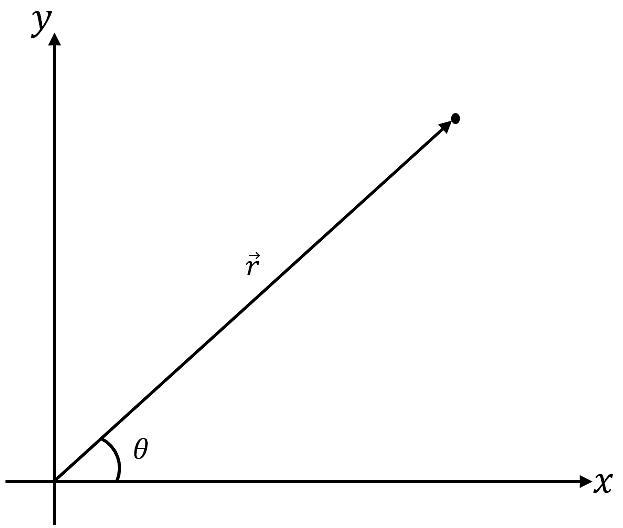
\includegraphics[width=3.3125in,height=2.95764in]{Imagenes/media/image28.png}

Ahora se procede a hallar la base para esta trayectoria:

\[\widehat{a_{r}} = \frac{\frac{\partial\overrightarrow{r}}{\partial r}}{\left| \frac{\partial\overrightarrow{r}}{\partial r} \right|} = \cos{\omega t\ \widehat{a_{x}}} + {sen}{\omega t\ \widehat{a_{y}}}\]

\[\widehat{a_{\theta}} = \frac{\frac{\partial\overrightarrow{r}}{\partial\theta}}{\left| \frac{\partial\overrightarrow{r}}{\partial\theta} \right|} = - {sen}{\omega t\ \widehat{a_{x}}} + \cos{\omega t\ \widehat{a_{y}}}\]

Luego:

\[\overrightarrow{r}(t) = A\widehat{a_{r}}\]

\[\overrightarrow{\dot{r}}(t) = A\dot{\widehat{a_{r}}}\]

Donde \(\dot{\widehat{a_{r}}} = \omega\widehat{a_{\theta}}\) de esta
manera:

\[\overrightarrow{\dot{\mathbf{r}}}\mathbf{(t) =}\mathbf{A}\mathbf{\omega}\widehat{\mathbf{a}_{\mathbf{\theta}}}\]

\[\overrightarrow{\ddot{\mathbf{r}}}\left( \mathbf{t} \right)\mathbf{=}\mathbf{- A}\mathbf{\omega}^{\mathbf{2}}\widehat{\mathbf{a}_{\mathbf{r}}}\]

Es de notar que
\(\overrightarrow{r}(t)\mathbf{\bot}\overrightarrow{\dot{r}}(t)\) y
\(\overrightarrow{\dot{r}}(t)\mathbf{\bot}\overrightarrow{\ddot{r}}(t)\).

\textbf{Ejemplo 2:} Hallar las componentes covariantes de la velocidad
para las coordenadas cilíndricas.

\textbf{Solución:} En primer lugar se sabe que las componentes
covariantes de la velocidad están dadas por:

\[V_{i} = \frac{\partial}{\partial\dot{q_{i}}}\left( \frac{1}{2}v^{2} \right)\]

Por otro lado el vector velocidad para las coordenadas cilíndricas se
escribe como:

\[\overrightarrow{\dot{r}} = \dot{\rho}\widehat{a_{\rho}} + \rho\dot{\phi}\widehat{a_{\phi}} + \dot{z}\widehat{a_{z}}\]

De donde:

\[v^{2} = {\dot{\rho}}^{2} + \rho^{2}{\dot{\phi}}^{2} + {\dot{z}}^{2}\]

Nótese que \(\rho\), \(\phi\) y \(z\) juegan el papel de coordenadas
generalizadas, es decir \(q_{i},\ \)así:

\[V_{i1,2,\ \ 3} = \frac{\partial}{\partial\dot{q_{i}}}\left( \frac{{\dot{\rho}}^{2} + \rho^{2}{\dot{\phi}}^{2} + {\dot{z}}^{2}}{2} \right)\]

\[V_{1} = \frac{\partial}{\partial\dot{\rho}}\left( \frac{{\dot{\rho}}^{2} + \rho^{2}{\dot{\phi}}^{2} + {\dot{z}}^{2}}{2} \right)\mathbf{=}\dot{\rho}\]

\[V_{2} = \frac{\partial}{\partial\dot{\phi}}\left( \frac{{\dot{\rho}}^{2} + \rho^{2}{\dot{\phi}}^{2} + {\dot{z}}^{2}}{2} \right) = \rho^{2}\dot{\phi}\]

\[V_{3} = \frac{\partial}{\partial\dot{z}}\left( \frac{{\dot{\rho}}^{2} + \rho^{2}{\dot{\phi}}^{2} + {\dot{z}}^{2}}{2} \right) = \dot{z}\]

\(V_{1}\), \(V_{2}\) y \(V_{3}\) corresponde a las componentes
covariantes de la velocidad para las coordenadas cilíndricas.

Ejercicio: Hallar las componentes covariantes para la aceleración de las
coordenadas cilíndricas. \(\therefore\)

\[\mathbf{a}_{\mathbf{i}}\mathbf{=}\frac{\mathbf{d}}{\mathbf{dt}}\frac{\mathbf{\partial}}{\mathbf{\partial}\dot{\mathbf{q}_{\mathbf{i}}}}\left( \frac{\mathbf{1}}{\mathbf{2}}\mathbf{v}^{\mathbf{2}} \right)\mathbf{-}\frac{\mathbf{\partial}}{\mathbf{\partial}\mathbf{q}_{\mathbf{i}}}\left( \frac{\mathbf{1}}{\mathbf{2}}\mathbf{v}^{\mathbf{2}} \right)\]

\textbf{Capítulo 2 Dinámica de Lagrange}

Joseph-Louis Lagrange, nació en Turín el 25 de enero de 1736 y murió en
París el 10 de Abril de 1813, fue
un~\href{https://es.wikipedia.org/wiki/F\%C3\%ADsico}{físico},~\href{https://es.wikipedia.org/wiki/Matem\%C3\%A1tico}{matemático}~y~\href{https://es.wikipedia.org/wiki/Astr\%C3\%B3nomo}{astrónomo}~franco
italiano que después vivió
en~\href{https://es.wikipedia.org/wiki/Prusia}{Prusia}~y~\href{https://es.wikipedia.org/wiki/Francia}{Francia}.

Lagrange trabajó
en~\href{https://es.wikipedia.org/wiki/Berl\%C3\%ADn}{Berlín}~durante
veinte años
para~\href{https://es.wikipedia.org/wiki/Federico_II_el_Grande}{Federico
II de Prusia}. Aportó avances transcendentales en múltiples ramas de las
matemáticas, desarrolló
la~\href{https://es.wikipedia.org/wiki/Mec\%C3\%A1nica_Lagrangiana}{mecánica
Lagrangiana}~y fue el autor de novedosos trabajos
de~\href{https://es.wikipedia.org/wiki/Astronom\%C3\%ADa}{astronomía}.
Tanto por la importancia como por el volumen de sus contribuciones
científicas se le puede considerar uno de los físicos y matemáticos más
destacados de la historia.

Uno de los trabajos más importantes realizados por Lagrange fue el de
reformular la mecánica clásica Newtoniana con la finalidad de reducir
fórmulas y facilitar cálculos. Este desarrollo fue realizado entre 1772
y 1788 el cual recibió el nombre de \emph{Mecánica Lagrangiana} lo cual
conlleva a la mecánica analítica. En su trabajo alberga, modifica y
generaliza conocimientos que viene dados desde Newton. El tratamiento
realizado por Lagrange en el campo de las ecuaciones diferenciales en la
mecánica representa uno de los logros más representativos en esta
disciplina. Dentro de su desarrollo se encuentra el principio de los
trabajos virtuales donde hace de este principio un principio
fundamental, por otro lado se encuentra la deducción de la mecánica de
fluidos y sólidos mediante el cálculo diferencial.

De todo este trabajo uno de los objetivos es mostrar la inclusión de la
mecánica a través de un único principio el cual permite generalizar
fórmulas que por consiguiente dan un resultado en particular. Quizás
dentro del resultado más inteligente del análisis de Lagrange fue la
utilización del método de las coordenadas generalizadas, él consideró a
diferencia de d'Alembert y Euler quienes consideraban seguir el
movimiento de cada parte individual de un sistema que era más factible
considerar la configuración de dicho sistema por una cantidad suficiente
de variables donde esta cantidad corresponde a los grados de libertad
que posee el sistema, a partir de esto se pueden tener las energías
cinética y potencial del sistema mediante el uso de estas coordenadas de
donde a través del uso de la diferenciación se obtienen las ecuaciones
diferenciales.

Entre otros teoremas menores aquí dados se puede mencionar la
proposición de que la energía cinética de un sistema material bajo las
restricciones dadas es un máximo, y
el~\href{https://es.wikipedia.org/wiki/Principio_de_m\%C3\%ADnima_acci\%C3\%B3n}{principio
de mínima acción}. Todo el análisis es tan elegante
que~\href{https://es.wikipedia.org/wiki/William_Rowan_Hamilton}{William
Rowan Hamilton}~dijo que este trabajo «solo podría describirse como un
poema científico». Puede ser interesante observar que Lagrange comentó
que la mecánica realmente era una rama de la matemática pura, análoga a
una geometría de cuatro dimensiones, a saber, el tiempo y las tres
coordenadas del punto en el espacio.

\textbf{DEDUCCIÓN DE LA ECUACIÓN DE MOVIMIENTO DE LAGRANGE}

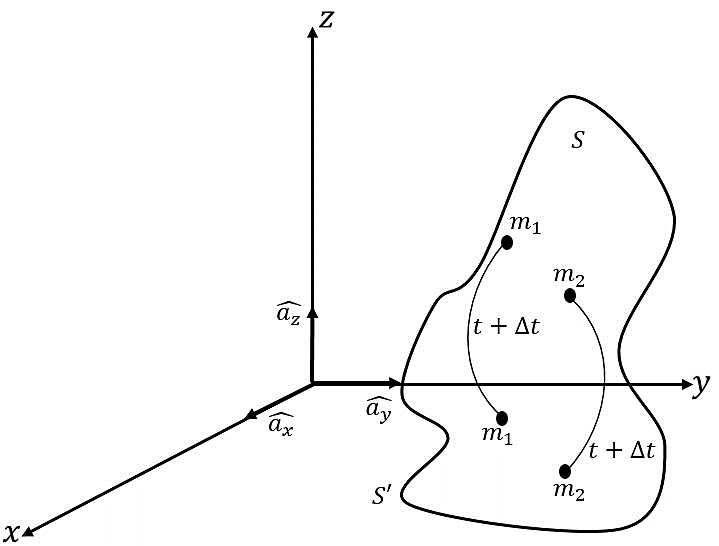
\includegraphics[width=5.78819in,height=4.39583in]{Imagenes/media/image29.png}Considérese
un sistema \(S\) de dos partículas \(m_{1}\) y \(m_{2}\) que evolucionan
de \(t\ \)a \(t + \mathrm{\Delta}t\):

Una condición física necesaria para manipular este sistema es que \(S\)
no interactúe con \(S'\).\\
Tomando el momento lineal dado por:

\[\overrightarrow{p} = m\overrightarrow{v}\]

Si se da que \(\overrightarrow{p} = cte\) el momento lineal se conserva
y se manifiesta la primera Ley de Newton. Así mismo, al no considerar
efectos relativistas donde las masas no cambian se cumple que:

\[{\overrightarrow{p}}_{T} = {\overrightarrow{p}}_{1} + {\overrightarrow{p}}_{2} = cte\]

\[m_{1}{\overrightarrow{v}}_{1i} + m_{2}{\overrightarrow{v}}_{2i} = m_{1}{\overrightarrow{v}}_{1} + m_{2}{\overrightarrow{v}}_{2}\]

\[{- m}_{1}\left( {\overrightarrow{v}}_{1} - {\overrightarrow{v}}_{1i} \right) = m_{2}\left( {\overrightarrow{v}}_{2} - {\overrightarrow{v}}_{2i} \right)\]

\[m_{1}\mathrm{\Delta}{\overrightarrow{v}}_{1} = - m_{2}\mathrm{\Delta}{\overrightarrow{v}}_{2}\]

\[\frac{m_{1}}{m_{2}} = \frac{\left| \mathrm{\Delta}{\overrightarrow{v}}_{2} \right|}{\left| \mathrm{\Delta}{\overrightarrow{v}}_{1} \right|} \rightarrow \mathbf{m}_{\mathbf{1}}\mathbf{=}\mathbf{m}_{\mathbf{2}}\frac{\left| \mathbf{\mathrm{\Delta}}{\overrightarrow{\mathbf{v}}}_{\mathbf{2}} \right|}{\left| \mathbf{\mathrm{\Delta}}{\overrightarrow{\mathbf{v}}}_{\mathbf{1}} \right|}\]

El resultado de la expresión (53) se denomina \emph{masa dinámica.}

Tomando el límite cuando \(\mathrm{\Delta}t\) tiende a cero en la
ecuación (52) se tiene que:

\[\lim_{\mathrm{\Delta}t \rightarrow 0}\left( \frac{m_{1}\mathrm{\Delta}{\overrightarrow{v}}_{1}}{\mathrm{\Delta}t} = - \frac{m_{2}\mathrm{\Delta}{\overrightarrow{v}}_{2}}{\mathrm{\Delta}t} \right)\]

Se puede ver que la expresión es la definición de una derivada por lo
que se puede reescribir como:

\[m_{1}\frac{d{\overrightarrow{v}}_{1}}{dt} = - m_{2}\frac{d{\overrightarrow{v}}_{2}}{dt}\]

\[\frac{d}{dt}\left( m_{1}{\overrightarrow{v}}_{1} \right) = - \frac{d}{dt}\left( m_{2}{\overrightarrow{v}}_{2} \right)\]

\[\frac{\mathbf{d}{\overrightarrow{\mathbf{p}}}_{\mathbf{1}}}{\mathbf{dt}}\mathbf{= -}\frac{\mathbf{d}{\overrightarrow{\mathbf{p}}}_{\mathbf{2}}}{\mathbf{dt}}\]

La ecuación (54) corresponde a la tercera Ley de Newton lo que conlleva
fácilmente a tener la segunda Ley de Newton:

\[\overrightarrow{\mathbf{F}}\mathbf{=}\frac{\mathbf{d}\overrightarrow{\mathbf{p}}}{\mathbf{dt}}\mathbf{= m}\overrightarrow{\mathbf{a}}\]

Se procede ahora a introducir la fuerza generalizada dada por:

\[ma_{i} = m\frac{d}{dt}\frac{\partial}{\partial\dot{q_{i}}}\left( \frac{1}{2}v^{2} \right) - m\frac{\partial}{\partial q_{i}}\left( \frac{1}{2}v^{2} \right)\]

\[ma_{i} = \frac{d}{dt}\frac{\partial}{\partial\dot{q_{i}}}\left( \frac{1}{2}{mv}^{2} \right) - \frac{\partial}{\partial q_{i}}\left( \frac{1}{2}{mv}^{2} \right)\]

Sea \(ma_{i} = Q_{i}\) la fuerza generalizada y sea
\(\frac{1}{2}{mv}^{2} = T\) la energía cinética:

\[\mathbf{Q}_{\mathbf{i}}\mathbf{=}\frac{\mathbf{d}}{\mathbf{dt}}\frac{\mathbf{\partial T}}{\mathbf{\partial}\dot{\mathbf{q}_{\mathbf{i}}}}\mathbf{-}\frac{\mathbf{\partial T}}{\mathbf{\partial}\mathbf{q}_{\mathbf{i}}}\]

La expresión (56) aplica únicamente para sistemas conservativos. Por
otro lado:

\[Q_{i} = \left( F_{x}\widehat{a_{x}} + F_{y}\widehat{a_{y}}{+ F}_{z}\widehat{a_{z}} \right) \cdot \left( \frac{\partial x}{\partial q_{i}}\widehat{a_{x}} + \frac{\partial y}{\partial q_{i}}\widehat{a_{y}} + \frac{\partial z}{\partial q_{i}}\widehat{a_{z}} \right)\]

\[Q_{i} = F_{x}\frac{\partial x}{\partial q_{i}} + F_{y}\frac{\partial y}{\partial q_{i}} + F_{z}\frac{\partial z}{\partial q_{i}}\]

Si \(\overrightarrow{F}\) es conservativa
\(\overrightarrow{F} = - \overrightarrow{\nabla}U\).

Donde \(U\) representa la energía potencial, así:

\[\overrightarrow{F} = - \left( \frac{\partial U}{\partial x}\widehat{a_{x}} + \frac{\partial U}{\partial y}\widehat{a_{y}} + \frac{\partial U}{\partial z}\widehat{a_{z}} \right)\]

Por lo tanto la fuerza generalizada se puede reescribir como:

\[Q_{i} = - \frac{\partial U}{\partial x}\frac{\partial x}{\partial q_{i}} - \frac{\partial U}{\partial y}\frac{\partial y}{\partial q_{i}} - \frac{\partial U}{\partial z}\frac{\partial z}{\partial q_{i}}\]

\[Q_{i} = - \frac{\partial U}{\partial q_{i}}\]

Luego; la ecuación (56) toma la forma:

\[- \frac{\partial U}{\partial q_{i}} = \frac{d}{dt}\frac{\partial T}{\partial\dot{q_{i}}} - \frac{\partial T}{\partial q_{i}}\]

Reescribiendo:

\[\frac{d}{dt}\frac{\partial}{\partial\dot{q_{i}}}(T - U) - \frac{\partial}{\partial q_{i}}(T - U) = 0\]

Por teoría a la mano se puede definir \(T - U = L\) lo que se denomina
LAGRANGIANO DEL SISTEMA, finalmente:

\[\frac{\mathbf{d}}{\mathbf{dt}}\frac{\mathbf{\partial L}}{\mathbf{\partial}\dot{\mathbf{q}_{\mathbf{i}}}}\mathbf{-}\frac{\mathbf{\partial L}}{\mathbf{\partial}\mathbf{q}_{\mathbf{i}}}\mathbf{= 0}\]

La ecuación (57) corresponde a una de las ecuaciones más importantes de
la mecánica clásica.

\textbf{FUERZAS DE LIGADURA Y ECUACIONES DE SUPERFICIES}

Clásicamente en la formulación de la mecánica, expresar matemáticamente
un fenómeno de modo que
las~\href{https://es.wikipedia.org/wiki/Fuerza}{fuerzas}~no aparezcan
explícitamente es el problema, debido a que muchas veces aparte de las
condiciones iniciales lo que no se conoce precisamente es cuales son
todas las fuerzas que actúan sobre el sistema. Es ahí donde surgen las
fuerzas de ligadura, o simplemente ligaduras, cuando por ejemplo se
tiene alguna partícula que tenga que moverse por un camino específico.
Si estas fuerzas de ligadura se conocieran simplemente se las sumaría
con las demás fuerzas, pero el problema radica que por lo general se
conocen éstas ligaduras y no las fuerzas resultantes en el sistema.

Las fuerzas de ligadura generalmente están dadas por la ecuación general
de una superficie las cuales pueden escribirse como:

\[q_{1} = q_{1}(x,\ y,\ z;t) = C_{1} = \Phi_{1}\]

\[q_{2} = q_{2}(x,\ y,\ z;t) = C_{2} = \Phi_{2}\]

\[q_{3} = q_{3}(x,\ y,\ z;t) = C_{3} = \Phi_{3}\]

La intersección de las tres superficies es un punto en común:

\(\Phi = \Phi(x,\ y,\ z;t) = C\) (58)

La ecuación (58) corresponde a la ecuación general de una superficie.
Las fuerzas de ligadura pueden clasificarse mediante dos criterios; de
acuerdo a la aparición explícita del tiempo o no; y de acuerdo la
integralidad o no, este último permite o no reducir los grados de
libertad. Se denominan \emph{ligaduras esclerónomas} cuando las
ligaduras son independientes del tiempo y \emph{ligaduras reónomas}
cuando contienen al tiempo explícitamente, es decir, son dependientes
del tiempo. Por otro lado, se denominan \emph{ligaduras holónomas} si
estas permiten reducir el número de grados de libertad; en caso
contrario se denominan \emph{ligaduras no holónomas.} Si se toman los
vectores perpendiculares:

\[\overrightarrow{\nabla}q_{j} = {\overrightarrow{B}}_{j}\]

Las fuerzas normales o perpendiculares a las superficies se obtienen de
la base recíproca, por lo que la fuerza normal está dada por:

\[\overrightarrow{R} = \lambda_{j}\overrightarrow{\nabla}\Phi_{j}\]

\(\overrightarrow{R}\) representa la fuerza normal y \(\lambda_{j}\)
representa los llamados \emph{multiplicadores de Lagrange.} Para las
componentes covariantes de la fuerza normal se tiene:

\[\overrightarrow{\mathbf{R}} = \sum_{i = 1}^{}\left( \overrightarrow{R} \cdot \overrightarrow{b_{i}} \right)\overrightarrow{B_{j}}\]

\[R_{\mathbf{i}} = \sum_{i = 1}^{}{\overrightarrow{R} \cdot \overrightarrow{b_{i}}} = \sum_{i = 1}^{}\lambda_{j}\left( \frac{\partial\Phi_{j}}{\partial x}\widehat{a_{x}} + \frac{\partial\Phi_{j}}{\partial y}\widehat{a_{y}} + \frac{\partial\Phi_{j}}{\partial z}\widehat{a_{z}} \right) \cdot \left( \frac{\partial x}{\partial q_{i}}\widehat{a_{x}} + \frac{\partial y}{\partial q_{i}}\widehat{a_{y}} + \frac{\partial z}{\partial q_{i}}\widehat{a_{z}} \right)\]

\[R_{\mathbf{i}} = \sum_{i = 1}^{}\lambda_{j}\left( \frac{\partial\Phi_{j}}{\partial x}\frac{\partial x}{\partial q_{i}} + \frac{\partial\Phi_{j}}{\partial y}\frac{\partial y}{\partial q_{i}} + \frac{\partial\Phi_{j}}{\partial z}\frac{\partial z}{\partial q_{i}} \right)\]

\[\mathbf{\ \ \ \ \ \ \ \ \ \ \ \ \ \ \ \ \ \ \ \ \ \ \ \ \ \ \ \ \ \ \ \ \ \ \ \ \ \ \ \ \ \ \ \ \ \ \ \ \ \ \ \ \ \ \ \ \ \ \ \ \ }R_{\mathbf{i}}\mathbf{=}\sum_{\mathbf{i = 1}}^{}{\mathbf{\lambda}_{\mathbf{j}}\frac{\mathbf{\partial}\mathbf{\Phi}_{\mathbf{j}}}{\mathbf{\partial}\mathbf{q}_{\mathbf{i}}}}\]

Si se introducen las componentes covariantes de la aceleración se puede
escribir la ecuación de movimiento de Lagrange en términos de las
fuerzas de ligadura y los multiplicadores de Lagrange, así:

\[\overrightarrow{a} = \sum_{i = 1}^{3}(\overrightarrow{a} \cdot \overrightarrow{b_{i}})\ \overrightarrow{B_{j}}\]

\[a_{i} = \left( \ddot{x}\widehat{a_{x}} + \ddot{y}\widehat{a_{y}} + \ddot{z}\widehat{a_{z}} \right) \cdot \left( \frac{\partial x}{\partial q_{i}}\widehat{a_{x}} + \frac{\partial y}{\partial q_{i}}\widehat{a_{y}} + \frac{\partial z}{\partial q_{i}}\widehat{a_{z}} \right)\]

\[a_{i} = \ddot{x}\frac{\partial x}{\partial q_{i}} + \ddot{y}\frac{\partial y}{\partial q_{i}} + \ddot{z}\frac{\partial z}{\partial q_{i}}\]

\[Q_{i} = ma_{i} = \frac{d}{dt}\frac{\partial}{\partial\dot{q_{i}}}\left( \frac{1}{2}{mv}^{2} \right) - \frac{\partial}{\partial q_{i}}\left( \frac{1}{2}{mv}^{2} \right)\]

\[Q_{i} = \frac{d}{dt}\frac{\partial T}{\partial\dot{q_{i}}} - \frac{\partial T}{\partial q_{i}}\]

De esta manera:

\[{\frac{d}{dt}\frac{\partial T}{\partial\dot{q_{i}}} - \frac{\partial T}{\partial q_{i}} = Q}_{i} + \sum_{i = 1}^{}{\lambda_{j}\frac{\partial\Phi_{j}}{\partial q_{i}}}\]

\[{\frac{\mathbf{d}}{\mathbf{dt}}\frac{\mathbf{\partial T}}{\mathbf{\partial}\dot{\mathbf{q}_{\mathbf{i}}}}\mathbf{-}\frac{\mathbf{\partial T}}{\mathbf{\partial}\mathbf{q}_{\mathbf{i}}}\mathbf{= Q}}_{\mathbf{i}}\mathbf{+}\mathbf{R}_{\mathbf{i}}\]

\textbf{PRINCIPIO DE LOS TRABAJOS VIRTUALES}

Supóngase un sistema de \(n\)-partículas en equilibrio y supóngase
además una variación configuracional de las coordenadas del sistema, tal
como se muestra en la \emph{figura 14}. La variación configuracional de
las coordenadas se refieren a una variación en un instante de tiempo
(las fuerzas externas y de ligadura no cambian). Este desplazamiento que
ocurre en un instante de tiempo se le llama desplazamiento virtual. Este
desplazamiento virtual se diferencia del desplazamiento real puesto que
este último se da cuando a lo largo de la trayectoria al derivar con
respecto al parámetro de tiempo \(t\) (el vector apunta siempre en la
dirección de movimiento) mientras que el desplazamiento virtual aparece
cuando se deriva con respecto a un parámetro \(\epsilon\) que para
distintas trayectorias de movimiento que varían de una manera apropiada
con las ligaduras del sistema tiene una enumeración.

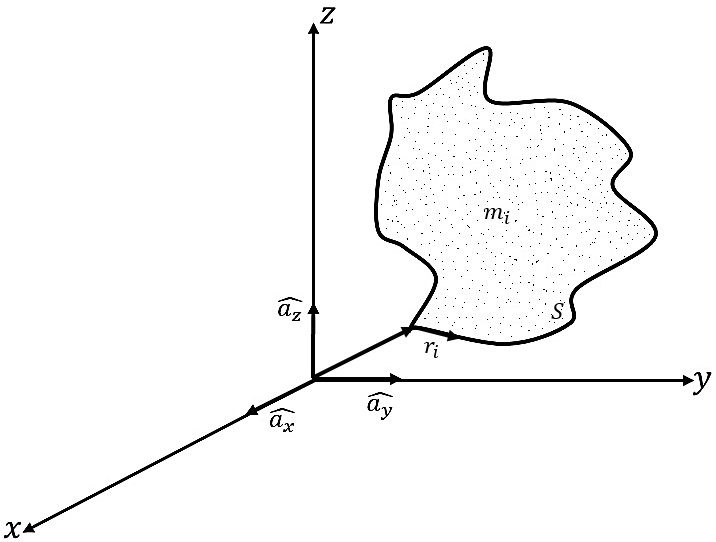
\includegraphics[width=6.34375in,height=4.80211in]{Imagenes/media/image30.jpeg}Para
denotar la derivada que concierne a:

se utiliza con frecuencia el símbolo \(\delta\). Por la definición de
trabajo se tiene para el \emph{principio de los trabajos virtuales} que:

\[\sum_{i}^{}{\overrightarrow{F_{i}} \cdot \delta\overrightarrow{r_{i}} = 0}\]

Reescribiendo:

\[\sum_{i}^{}{\left( {\overrightarrow{F_{i}}}^{(a)} + \overrightarrow{F_{1i}} \right) \cdot \delta\overrightarrow{r_{i}} = 0}\]

\[\sum_{i}^{}{{\overrightarrow{F_{i}}}^{(a)} \cdot \delta\overrightarrow{r_{i}} + \overrightarrow{F_{1i}} \cdot \delta\overrightarrow{r_{i}} = 0}\]

En la ecuación (61) no se va a considerar el segundo término ya que se
tiene un sistema que se encuentra en equlibrio, de esta manera:

\[\sum_{i}^{}{\overrightarrow{F_{i}} \cdot \delta\overrightarrow{r_{i}} = 0}\]

La expresión (62) denota una fuerza invertida. Si se escribe la segunda
ley de Newton como:

\[\overrightarrow{F_{i}} = \overrightarrow{\dot{p_{i}}}\]

y se lleva a la ecuación (62) se da que:

\[\sum_{\mathbf{i}}^{}{\left( \overrightarrow{\mathbf{F}_{\mathbf{i}}}\mathbf{-}\overrightarrow{\dot{\mathbf{p}_{\mathbf{i}}}} \right)\mathbf{\cdot \delta}\overrightarrow{\mathbf{r}_{\mathbf{i}}}\mathbf{= 0}}\]

La expresión (62) corresponde al \emph{principio de D'Alembert.} Este
principio es considerado una generalización de la segunda ley de Newton
que se puede aplicar de algún modo a sistemas con ligaduras, se
aprovecha de la condición de que las fuerzas de ligadura no realizan
trabajo en un movimiento compatible.

Es de notar que \(\delta\overrightarrow{r_{i}}\) hacen el papel de las
\(\delta\overrightarrow{q_{j}}\) que no son independientes.

Tomando ahora el vector posición escrito como:

\[{\overrightarrow{r}}_{i} = r_{i}\left( q_{1},\ q_{2},q_{3},\ldots q_{j};t \right)\]

\(q_{1},\ q_{2},q_{3},\ldots\) son coordenadas generalizadas
independientes, aplicando \(\delta\) en el vector
\({\overrightarrow{r}}_{i}\), se tiene:

\[\delta{\overrightarrow{r}}_{i} = \sum_{j}^{}\frac{\partial r_{i}}{\partial q_{j}}\delta q_{j}\]

\[\delta{\overrightarrow{r}}_{i} = \frac{\partial r_{i}}{\partial q_{1}}\delta q_{1} + \frac{\partial r_{i}}{\partial q_{2}}\delta q_{2} + \frac{\partial r_{i}}{\partial q_{3}}\delta q_{3} + \ldots\]

De este modo:

\[\sum_{i,j}^{}{\left( \overrightarrow{\mathbf{F}_{\mathbf{i}}}\mathbf{-}\overrightarrow{\dot{\mathbf{p}_{\mathbf{i}}}} \right).\frac{\partial r_{i}}{\partial q_{j}}}\delta q_{j} = 0\]

\[- \sum_{i,j}^{}{\overrightarrow{\dot{p_{i}}.}\frac{\partial r_{i}}{\partial q_{j}}}\delta q_{j} + \sum_{i,j}^{}{\overrightarrow{F_{i}}.\frac{\partial r_{i}}{\partial q_{j}}\delta q_{j}} = 0\]

Nótese que:

\[\sum_{i,j}^{}{\overrightarrow{F_{i}}.\frac{\partial r_{i}}{\partial q_{j}} = Q_{j} \rightarrow \sum_{i}^{}{\overrightarrow{F_{i}} \cdot {\overrightarrow{b}}_{i} = Q_{j}}}\]

La expresión (65) corresponde a la fuerza generalizada también llamada
componentes covariantes de la fuerza. Por otro lado:

\[\sum_{i,j}^{}{\overrightarrow{\dot{p_{i}}} \cdot \frac{\partial\overrightarrow{r_{i}}}{\partial q_{j}}} = \sum_{i,j}^{}{m_{i}\overrightarrow{\ddot{r_{i}}} \cdot \frac{\partial\overrightarrow{r_{i}}}{\partial q_{j}}} = \sum_{i,\ j}^{}{m_{i}\frac{d{\overrightarrow{\dot{r}}}_{i}}{dt} \cdot \frac{\partial\overrightarrow{r_{i}}}{\partial q_{j}}}\]

\[\sum_{i,\ j}^{}{m_{i}\frac{d}{dt}\left( {\overrightarrow{\dot{r}}}_{i} \cdot \frac{\partial\overrightarrow{r_{i}}}{\partial q_{j}} \right) =}\sum_{i,j}^{}{m_{i}\overrightarrow{\ddot{r_{i}}} \cdot \frac{\partial\overrightarrow{r_{i}}}{\partial q_{j}}} + \sum_{i,\ j}^{}m_{i}{\overrightarrow{\dot{r}}}_{i} \cdot \frac{d}{dt}\left( \frac{\partial\overrightarrow{r_{i}}}{\partial q_{j}} \right)\]

\[\frac{d}{dt}\sum_{i,\ j}^{}m_{i}\left( {\overrightarrow{\dot{r}}}_{i} \cdot \frac{\partial\overrightarrow{\dot{r_{i}}}}{\partial\dot{q_{j}}} \right) - \sum_{i,\ j}^{}m_{i}{\overrightarrow{\dot{r}}}_{i} \cdot \frac{d}{dt}\left( \frac{\partial\overrightarrow{r_{i}}}{\partial q_{j}} \right) = \sum_{i,\ j}^{}{m_{i}\overrightarrow{\ddot{r_{i}}}} \cdot \frac{\partial\overrightarrow{r_{i}}}{\partial q_{j}}\]

Reescribiendo se cumple que:

\[\sum_{i,j}^{}{m_{i}\overrightarrow{\ddot{r_{i}}} \cdot \frac{\partial\overrightarrow{r_{i}}}{\partial q_{j}}} = \frac{d}{dt}\frac{\partial}{\partial\dot{q_{j}}}\left( \sum_{i}^{}{\frac{1}{2}m_{i}}{{\overrightarrow{\dot{r}}}_{i}}^{2} \right) - \frac{\partial}{\partial q_{j}}\left( \sum_{i}^{}{\frac{1}{2}m_{i}}{{\overrightarrow{\dot{r}}}_{i}}^{2} \right)\]

\[\sum_{j}^{}Q_{j}\delta q_{j} - \left\{ \sum_{j}^{}\left\lbrack \frac{d}{dt}\frac{\partial}{\partial\dot{q_{j}}}\left( \sum_{i}^{}{\frac{1}{2}m_{i}}{{\overrightarrow{\dot{r}}}_{i}}^{2} \right) - \frac{\partial}{\partial q_{j}}\left( \sum_{i}^{}{\frac{1}{2}m_{i}}{{\overrightarrow{\dot{r}}}_{i}}^{2} \right) \right\rbrack \right\}\delta q_{j} = 0\]

Como la energía cinética del sistema de \(n\)-partículas se escribe de
la forma:

\[T = \sum_{i}^{}{\frac{1}{2}m_{i}}{{\overrightarrow{\dot{r}}}_{i}}^{2}\]

Entonces:

\[\sum_{j}^{}\left\{ Q_{j} - \left\lbrack \frac{d}{dt}\frac{\partial T}{\partial\dot{q_{j}}} - \frac{\partial T}{\partial q_{j}} \right\rbrack \right\}\delta q_{j} = 0\]

\[Q_{j} - \left( \frac{d}{dt}\frac{\partial T}{\partial\dot{q_{j}}} - \frac{\partial T}{\partial q_{j}} \right) = 0\]

Finalmente:

\[\mathbf{Q}_{\mathbf{j}}\mathbf{=}\frac{\mathbf{d}}{\mathbf{dt}}\frac{\mathbf{\partial T}}{\mathbf{\partial}\dot{\mathbf{q}_{\mathbf{j}}}}\mathbf{-}\frac{\mathbf{\partial T}}{\mathbf{\partial}\mathbf{q}_{\mathbf{j}}}\]

La expresión (66) es otra manifestación de la ecuación de movimiento de
Lagrange en términos de las componentes covariantes de la fuerza, dada
para sistemas conservativos.

\textbf{Ejemplo 3:} Sobre la superficie de una superficie de sección
circular de radio \(R\) se deja caer una canica de masa \(m\) con
velocidad inicial nula y sin rozamiento, desde el punto considerado en
la superficie. Hallar el punto de despegue de la masa por el método de
los multiplicadores de Lagrange. Analizar el mismo problema si la
velocidad inicial de la masa es diferente de cero.

\textbf{Solución:} Considérese la situación mostrada en la \emph{figura
15}

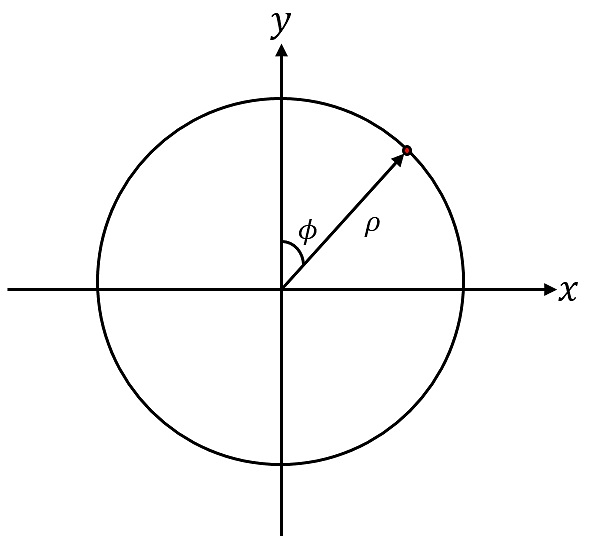
\includegraphics[width=4.97986in,height=4.625in]{Imagenes/media/image31.png}

Como se pide utilizar el método de los multiplicadores de Lagrange, se
tiene que:

\[\sum_{i = 1}^{}{\lambda_{j}\frac{\partial\Phi_{j}}{\partial q_{i}}} = \frac{d}{dt}\frac{\partial L}{\partial\dot{q_{i}}} - \frac{\partial L}{\partial q_{i}}\]

Además el sistema se considera sin rozamiento; entonces, el sistema es
conservativo, por lo que:

\[Q_{i} + \sum_{i = 1}^{}{\lambda_{j}\frac{\partial\Phi_{j}}{\partial q_{i}}} = \frac{d}{dt}\frac{\partial T}{\partial\dot{q_{i}}} - \frac{\partial T}{\partial q_{i}}\]

Ahora, es de tener en cuenta que de acuerdo a lo mostrado en la
\emph{figura 15} se hace conveniente trabajar con coordenadas polares,
haciendo las respectivas transformaciones se da que:

\[\cos\phi = \frac{y}{\rho} \rightarrow y = \rho\cos\phi\]

\[{sen}\phi = \frac{x}{\rho} \rightarrow x = \rho{sen}\phi\]

\[x^{2} + y^{2} = \rho^{2}\]

Se toma \(R^{2} = \rho^{2}\) en esta situación porque es la distancia
que corresponde al radio de la circunferencia antes de que la canica se
despegue de la superficie; en ese instante \(R^{2}\) es constante y
\(\rho^{2}\) es variable, por lo tanto la ecuación de ligadura va a
estar dada por:

\[\rho - R = 0 = \Phi(x,\ y;t)\]

Como solo hay una ecuación de ligadura se necesita únicamente un
multiplicador de Lagrange. A continuación se procede a obtener el
Lagrangiano del sistema dado por:

\[L = T - U\]

Para \(T\ \)se da que:

\[\dot{x} = \dot{\rho}{sen}\phi + \rho\dot{\phi}\cos\phi \rightarrow {\dot{x}}^{2} = {\dot{\rho}}^{2}{sen}^{2}\phi + 2\dot{\rho}\rho\dot{\phi}{sen}\phi\cos\phi + \rho^{2}{\dot{\phi}}^{2}\cos^{2}\phi\]

\[\dot{y} = \dot{\rho}\cos\phi - \rho\dot{\phi}{sen}\phi \rightarrow {\dot{y}}^{2} = {\dot{\rho}}^{2}\cos^{2}\phi - 2\dot{\rho}\rho\dot{\phi}\cos\phi{sen}\phi + \rho^{2}{\dot{\phi}}^{2}{sen}^{2}\phi\]

\[{\dot{x}}^{2} + {\dot{y}}^{2} = {\dot{\rho}}^{2} + \rho^{2}{\dot{\phi}}^{2}\]

De esta manera la energía cinética es:

\[\mathbf{T =}\frac{\mathbf{1}}{\mathbf{2}}\mathbf{m}\left( {\dot{\mathbf{\rho}}}^{\mathbf{2}}\mathbf{+}\mathbf{\rho}^{\mathbf{2}}{\dot{\mathbf{\phi}}}^{\mathbf{2}} \right)\]

Para la energía potencial \(U\ \)se tiene:

\[U = mgy\]

\[\mathbf{U = mg\rho}\mathbf{\cos}\mathbf{\phi}\]

Por lo tanto el Lagrangiano del sistema es:

\[\mathbf{L =}\frac{\mathbf{1}}{\mathbf{2}}\mathbf{m}\left( {\dot{\mathbf{\rho}}}^{\mathbf{2}}\mathbf{+}\mathbf{\rho}^{\mathbf{2}}{\dot{\mathbf{\phi}}}^{\mathbf{2}} \right)\mathbf{- mg\rho}\mathbf{\cos}\mathbf{\phi}\]

Luego, es necesario efectuar las operaciones necesarias para llevar las
correspondientes derivadas a la ecuación diferencial escrita en la
expresión (67), de esta manera:

\[\frac{\partial L}{\partial\dot{\rho}} = m\dot{\rho},\ \ \ \ \ \ \ \ \ \ \frac{\partial L}{\partial\rho} = m\rho{\dot{\phi}}^{2} - mg\cos\phi\]

\[\frac{\partial L}{\partial\dot{\phi}} = m\rho^{2}\dot{\phi},\ \ \ \ \frac{\partial L}{\partial\phi} = mg\rho{sen}\phi\ \ \ \ \ \ \ \ \ \ \ \ \ \ \ \ \]

Así, la ecuación (67) escrita para \(\rho\) y \(\dot{\rho}\) es:

\[\frac{d}{dt}\frac{\partial L}{\partial\dot{\rho}} - \frac{\partial L}{\partial\rho} = \lambda\frac{\partial\Phi}{\partial\rho},\ \ \ \ \ \ \ \ \frac{\partial\Phi}{\partial\rho} = 1\]

Por lo tanto; la ecuación de movimiento de Lagrange para \(\rho\) es:

\[\mathbf{\ }\frac{\mathbf{d}}{\mathbf{dt}}\left( \mathbf{m}\dot{\mathbf{\rho}} \right)\mathbf{- m\rho}{\dot{\mathbf{\phi}}}^{\mathbf{2}}\mathbf{+ mg}\mathbf{\cos}\mathbf{\phi}\mathbf{=}\mathbf{\lambda\ \ \ \ \ }\]

Por otro lado para \(\phi\) se da:

\[\frac{d}{dt}\frac{\partial L}{\partial\dot{\phi}} - \frac{\partial L}{\partial\phi} = \lambda\frac{\partial\Phi}{\partial\phi},\ \ \ \ \ \ \ \ \frac{\partial\Phi}{\partial\phi\ } = 0\]

\[\frac{d}{dt}\left( m\rho^{2}\dot{\phi} \right) - mg\rho{sen}\phi = 0\]

\[\mathbf{m}\mathbf{\rho}^{\mathbf{2}}\ddot{\mathbf{\phi}}\mathbf{+ 2}\mathbf{m\rho}\dot{\mathbf{\rho}}\dot{\mathbf{\phi}}\mathbf{- mg\rho}\mathbf{sen}\mathbf{\phi}\mathbf{= 0}\]

\uline{Condiciones Físicas para la Ecuación (68)}: Mientras la canica se
encuentra moviéndose sobre la superficie, existirá la fuerza de ligadura
\(\lambda \neq 0\), también es cierto que \(\rho = R,\)
\(\dot{\rho} = 0\) y \(\ddot{\rho} = 0\), por lo tanto:

\[- mR{\dot{\phi}}^{2} + mg\cos\phi = \lambda\]

En el momento del despegue ya no hay fuerzas de ligadura, así:

\[- mR{\dot{\phi}}^{2} + mg\cos\phi = 0\]

\[{\dot{\phi}}^{2} = \frac{mg\cos\phi}{mR}\]

\[{\dot{\mathbf{\phi}}}^{\mathbf{2}}\mathbf{=}\frac{\mathbf{g}}{\mathbf{R}}\mathbf{\cos}\mathbf{\phi}\]

\uline{Condiciones Físicas para la Ecuación (69)}: Mientras la partícula
se mueve en la superficie \(\rho = R\), \(\dot{\rho} = 0\) y
\(\ddot{\rho} = 0\), de este modo:

\[mR^{2}\ddot{\phi} - mgR{sen}{\phi = 0}\]

\[mR^{2}\ddot{\phi} = mgR{sen}\phi\]

\[\ddot{\mathbf{\phi}}\mathbf{=}\frac{\mathbf{g}}{\mathbf{R}}\mathbf{sen}\mathbf{\phi}\mathbf{\ \ \ \ \ \ \ \ \ \ }\]

Resolviendo para (71) se tiene:

\[\int_{0}^{\dot{\phi}}\ddot{\phi}\dot{\phi}dt = \int_{0}^{t}{\frac{g}{R}{sen}\phi}\dot{\phi}dt\]

Para el lado derecho de la igualdad se da que:

\[\int_{0}^{t}{\frac{g}{R}{sen}\phi}\dot{\phi}dt = \frac{g}{R}\int_{0}^{t}{{sen}\phi}\frac{d\phi}{dt}dt\]

\[\int_{0}^{t}{\frac{g}{R}{sen}\phi}\dot{\phi}dt = \frac{g}{R}\int_{0}^{\phi}{{sen}\phi}d\phi\]

\[\int_{\mathbf{0}}^{\mathbf{t}}{\frac{\mathbf{g}}{\mathbf{R}}\mathbf{sen}\mathbf{\phi}}\dot{\mathbf{\phi}}\mathbf{dt = -}\frac{\mathbf{g}}{\mathbf{R}}\left( \mathbf{\cos}\mathbf{\phi}\mathbf{- 1} \right)\mathbf{\ \ \ }\]

Para el lado izquierdo de la igualdad es necesario resolver la integral
por partes, sean \(\dot{\phi} = u\) y \(d\dot{\phi} = du\), así:

\[du = \frac{d}{dt}\left( \dot{\phi} \right)dt = \ddot{\phi}dt\]

Luego:

\[\int_{0}^{\phi}{udu =}\left. \ \frac{1}{2}{\dot{\phi}}^{2} \right\rfloor_{0}^{\phi}\ \ \ \ \ \ con\ \ \ \ \ \ {\dot{\phi}}^{2} = \frac{g}{R}\cos\phi\]

Finalmente; igualando la parte derecha y la parte izquierda de la
igualdad, se cumple que:

\[\frac{1}{2}\frac{g}{R}\cos\phi = - \frac{g}{R}\left( \cos\phi - 1 \right)\]

\[\cos\phi\left( \frac{1}{2} + 1 \right) = 1\]

\[\mathbf{\phi =}\mathbf{\cos}^{\mathbf{- 1}}\left( \frac{\mathbf{2}}{\mathbf{3}} \right)\]

Este será el ángulo con el que despegará la canica cuando la velocidad
inicial es igual a cero. Para obtener el ángulo con el que despegará
cuando la velocidad inicial es diferente de cero no es necesario
resolver todo el problema, únicamente se cambian los límites de
integración, de esta manera:

\[\left. \ \frac{1}{2}\dot{\phi^{2}} \right\rfloor_{{\dot{\phi}}_{0}}^{\dot{\phi}} = - \frac{g}{R}\left( \cos\phi - 1 \right)\]

\[\frac{1}{2}\dot{\phi^{2}} - \frac{1}{2}{{\dot{\phi}}_{0}}^{2} = - \frac{g}{R}\left( \cos\phi - 1 \right)\]

Es de notar que \({\dot{\phi}}_{0}\) se puede escribir como:

\[{\dot{\phi}}_{0} = \frac{V_{T}}{R}\]

De este modo:

\[\frac{1}{2}\dot{\phi^{2}} - \frac{1}{2}\frac{V_{T}}{R^{2}}^{2} = - \frac{g}{R}\left( \cos\phi - 1 \right)\ \ \ \ como\ \ \ \ {\dot{\phi}}^{2} = \frac{g}{R}\cos\phi\]

\[\frac{1}{2}\frac{g}{R}\cos\phi - \frac{1}{2}\frac{V_{T}}{R^{2}}^{2} = - \frac{g}{R}\left( \cos\phi - 1 \right)\]

\[\frac{g}{R}\cos\phi\left( \frac{1}{2} + 1 \right) = \frac{g}{R} + \frac{1}{2}\frac{V_{T}}{R^{2}}^{2}\]

\[\frac{3}{2}\frac{g}{R}\cos\phi = \frac{g}{R}\left( 1 + \frac{1}{2R}\frac{V_{T}}{g}^{2} \right)\]

\[\cos\phi = \frac{2}{3} + \frac{{V_{T}}^{2}}{3gR}\]

\[\mathbf{\phi =}\mathbf{\cos}^{\mathbf{- 1}}\left( \frac{\mathbf{2}}{\mathbf{3}}\mathbf{+}\frac{{\mathbf{V}_{\mathbf{T}}}^{\mathbf{2}}}{\mathbf{3}\mathbf{gR}} \right)\]

Este será el ángulo con el que se despegará la canica cuando la
velocidad inicial es diferentes de cero, es de notar que el primer
término del argumento del arcocoseno es el ángulo con que se despegará
la bolita cuando la velocidad inicial es igual a cero, por lo tanto se
puede concluir que para este caso el ángulo aumenta con respecto a la
aceleración centrípeta dada por la trayectoria circular descrita por la
canica.

\textbf{Ejemplo 4:} Considere un bloque de masa \(m\) moviéndose en un
plano inclinado sin fricción. Analizar la dinámica del sistema para
diferentes sistemas de observación.

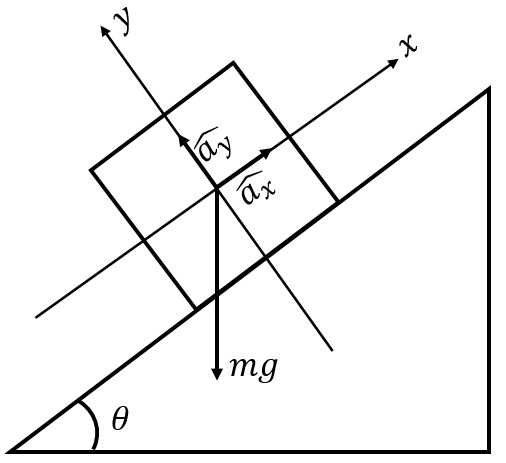
\includegraphics[width=3.23125in,height=2.95833in]{Imagenes/media/image32.jpeg}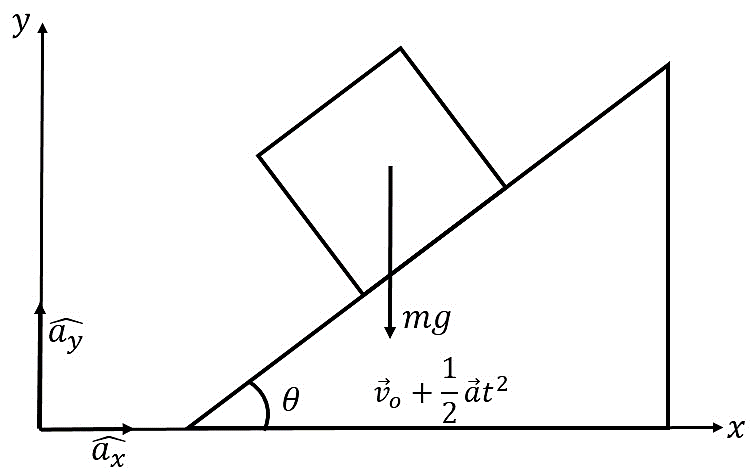
\includegraphics[width=5.34375in,height=3.35406in]{Imagenes/media/image33.png}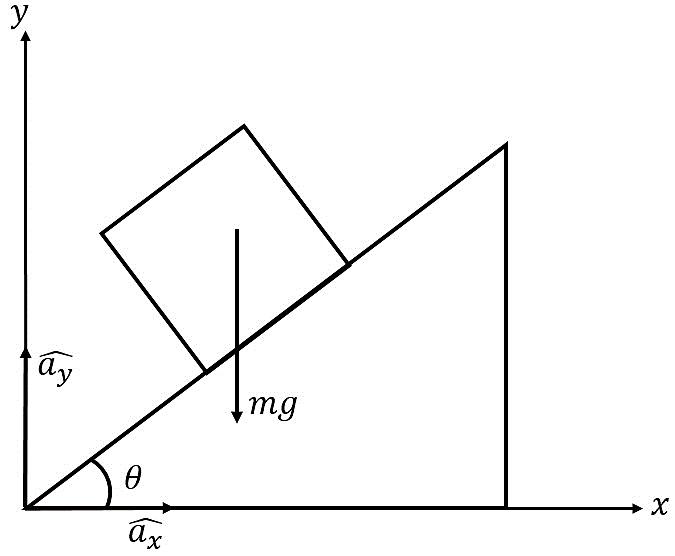
\includegraphics[width=3.41667in,height=2.80694in]{Imagenes/media/image34.png}

\textbf{Solución:} Inicialmente es de considerar que el bloque se mueve
sobre una curva por lo que se necesitan dos condiciones de ligaduras
(ecuaciones de superficie), por lo tanto van a aparecer dos
multiplicadores de Lagrange:

\[\Phi_{1} = y = 0\]

\[\Phi_{2} = z = 0\]

Para el caso a) se procede a utilizar:

\[Q_{i} + \mathbf{R}_{\mathbf{i}} = \frac{d}{dt}\frac{\partial T}{\partial\dot{q_{i}}} - \frac{\partial T}{\partial q_{i}}\]

Para lo cual la energía cinética va a estar dada por:

\[T = \frac{1}{2}m\left( {\dot{x}}^{2} + {\dot{y}}^{2} \right)\]

Las derivadas necesarias para llevar a la ecuación (73) son:

\[\frac{\partial T}{\partial\dot{x}} = m\dot{x},\ \ \ \ \ \ \ \ \ \ \frac{\partial T}{\partial x} = 0\]

\[\frac{\partial T}{\partial\dot{y}} = m\dot{y},\ \ \ \ \ \ \ \ \ \frac{\partial T}{\partial y} = 0\]

De esta manera:

\[\frac{d}{dt}\left( m\dot{x} \right) - 0 = - \ mg{sen}\theta + \lambda_{1}\frac{\partial\Phi_{1}}{\partial x} + \lambda_{2}\frac{\partial\Phi_{2}}{\partial x}\]

\[\frac{d}{dt}\left( m\dot{y} \right) - 0 = - \ mg\cos\theta + \lambda_{1}\frac{\partial\Phi_{1}}{\partial y} + \lambda_{2}\frac{\partial\Phi_{2}}{\partial y}\]

Como \(\Phi_{1} = y = 0\) y \(\Phi_{2} = z = 0\), entonces:

\[\frac{\partial\Phi_{1}}{\partial x} = 0,\ \ \ \ \ \ \ \ \frac{\partial\Phi_{2}}{\partial x} = 0\]

\[\frac{\partial\Phi_{1}}{\partial y} = 1,\ \ \ \ \ \ \ \ \frac{\partial\Phi_{2}}{\partial y} = 0\]

Por lo tanto:

\(m\ddot{x} = - \ mg{sen}\theta\)+\ldots{}\(\lambda_{1}(0)\)

\[\ddot{\mathbf{x}}\mathbf{= - \ g}\mathbf{sen}\mathbf{\theta}\]

Así mismo:

\[m\ddot{y} = - \ mg\cos\theta + \lambda_{1}\]

Para este caso \(y = 0\), \(\dot{y} = 0\) y \(\ddot{y} = 0\), por lo
tanto la solución va a estar dada por la condición de ligadura
\(\lambda_{1}\), así:

\[\mathbf{\lambda}_{\mathbf{1}}\mathbf{= mg}\mathbf{\cos}\mathbf{\theta}\]

Nótese que es la misma solución que se obtiene con mecánica Newtoniana.

Para el caso b) se hace conveniente usar:

\[Q_{i} + \sum_{i = 1}^{}{\lambda_{j}\frac{\partial\Phi_{j}}{\partial q_{i}}} = \frac{d}{dt}\frac{\partial T}{\partial\dot{q_{i}}} - \frac{\partial T}{\partial q_{i}}\]

Donde se tiene una ecuación de ligadura que está dada por:

\[\tan\theta = \frac{y}{x}\]

\[y - x\tan\theta = 0 = \Phi(x,y)\]

De esta manera la energía cinética se puede escribir como:

\[T = \frac{1}{2}m\left( {\dot{x}}^{2} + {\dot{y}}^{2} \right)\]

Así mismo:

\[\frac{\partial T}{\partial\dot{x}} = m\dot{x},\ \ \ \ \ \ \ \ \ \ \frac{\partial T}{\partial x} = 0\]

\[\frac{\partial T}{\partial\dot{y}} = m\dot{y},\ \ \ \ \ \ \ \ \ \frac{\partial T}{\partial y} = 0\]

Llevando esto a la ecuación (74) se tiene:

\[\frac{d}{dt}\left( m\dot{x} \right) - 0 = 0 + \lambda\frac{\partial\Phi}{\partial x}\]

\[\frac{d}{dt}\left( m\dot{y} \right) - 0 = - \ mg + \lambda\frac{\partial\Phi}{\partial y}\]

De este modo:

\[m\ddot{x} = - \ \lambda\tan\theta\]

\[m\ddot{y} = - \ mg + \lambda\]

Así:

\[m\ddot{x}\tan\theta = - \ mg + \lambda\]

Como \(m\ddot{x} = - \ \lambda\tan\theta\), entonces:

\[- \lambda\tan^{2}\theta = - \ mg + \lambda\]

\[\lambda\left( 1 + \tan^{2}\theta \right) = mg\]

\[\mathbf{\lambda =}\frac{\mathbf{mg}}{\mathbf{\sec}^{\mathbf{2}}\mathbf{\theta}}\]

\(\lambda\) no es la fuerza de ligadura, hay que obtener su norma; de
esta manera:

\[\left| \overrightarrow{R} \right| = \sqrt{\lambda^{2} + \lambda^{2}\tan^{2}\theta}\]

\[\left| \overrightarrow{R} \right| = \sqrt{\lambda^{2}(1 + \tan^{2}\theta)}\]

\[\left| \overrightarrow{R} \right| = \sqrt{\lambda^{2}\sec^{2}\theta}\]

\[\left| \overrightarrow{R} \right| = \lambda\sec\theta\]

\[\lambda = \frac{mg}{\sec^{2}\theta}\]

Finalmente:

\[\left| \overrightarrow{R} \right| = \frac{mg}{\sec^{2}\theta}\sec\theta\]

\[\left| \overrightarrow{\mathbf{R}} \right|\mathbf{= mg}\mathbf{\cos}\mathbf{\theta}\]

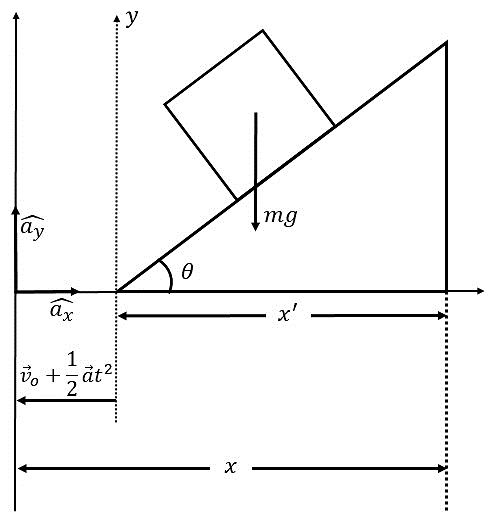
\includegraphics[width=5.0625in,height=4.76042in]{Imagenes/media/image35.png}Para
la situación c) se considera el sistema como un sistema no inercial:

Para esta situación la energía cinética está dada por:

\[T = \frac{1}{2}m\left( {\dot{x}}^{2} + {\dot{y}}^{2} \right)\]

Donde se tiene una ecuación de ligadura que está dada por:

\[\tan\theta = \frac{y}{x^{'}}\]

\[y - x^{'}\tan\theta = 0 = \Phi(x,y)\]

Como:

\[x^{'} = x - \left( {\overrightarrow{v}}_{o}t + \frac{1}{2}\overrightarrow{a}t^{2} \right)\]

Entonces la ecuación de ligadura se puede reescribir de la siguiente
forma:

\[y - \left( x - {\overrightarrow{v}}_{o}t - \frac{1}{2}\overrightarrow{a}t^{2} \right)\tan\theta = 0 = \Phi(x,y;t)\]

La condición de ligadura ya depende del tiempo. Las derivadas
correspondientes para llevar a la expresión (74) serán:

\[\frac{\partial T}{\partial\dot{x}} = m\dot{x},\ \ \ \ \ \ \ \ \ \ \frac{\partial T}{\partial x} = 0,\ \ \ \ \ \ \ \ \frac{\partial\Phi}{\partial x} = - \tan\theta\]

\[\frac{\partial T}{\partial\dot{y}} = m\dot{y},\ \ \ \ \ \ \ \ \ \frac{\partial T}{\partial y} = 0,\ \ \ \ \ \ \ \ \frac{\partial\Phi}{\partial y} = 1\ \ \ \ \ \ \ \ \ \ \ \ \]

De esta manera:

\[\frac{d}{dt}\left( m\dot{x} \right) - 0 = 0 + \lambda\frac{\partial\Phi}{\partial x}\]

\[\frac{d}{dt}\left( m\dot{y} \right) - 0 = - \ mg + \lambda\frac{\partial\Phi}{\partial y}\]

Así:

\[m\ddot{x} = - \ \lambda\tan\theta\]

\[m\ddot{y} = - \ mg + \lambda\]

\[y - x^{'}\tan\theta = 0 = \Phi(x,y)\]

\[y = x^{'}\tan\theta = \lbrack x - \left( {\overrightarrow{v}}_{o}t + \frac{1}{2}\overrightarrow{a}t^{2} \right)\rbrack\tan\theta\]

\[\ddot{y} = \left( \ddot{x} - a \right)\tan\theta\]

\[m\left( \ddot{x} - a \right)\tan\theta = - \ mg + \lambda\]

\[m\ddot{x}\tan\theta - ma\tan\theta = - \ mg + \lambda\]

Como \(m\ddot{x} = - \ \lambda\tan\theta\), entonces:

\[- \lambda\tan^{2}\theta - ma\tan\theta = - \ mg + \lambda\]

Reescribiendo, se tiene que:

\[m\left( g - a\tan\theta \right) = \lambda\left( 1 + \tan^{2}\theta \right)\]

\[m\left( g - a\tan\theta \right) = \lambda\sec^{2}\theta\]

Despejando la fuerza de ligadura \(\lambda:\)

\[\lambda = \frac{m\left( g - a\tan\theta \right)}{\sec^{2}\theta}\]

Por otro lado:

\[y = \left( x - {\overrightarrow{v}}_{o}t + \frac{1}{2}\overrightarrow{a}t^{2} \right)\tan\theta\]

\[\dot{y} = \left( x - {\overrightarrow{v}}_{o}t + \overrightarrow{a}t^{2} \right)\tan\theta\]

\[\ddot{y} = \left( \ddot{x} - a \right)\tan\theta\]

Obteniendo la magnitud de la condición de ligadura se cumple que:

\[\left| \overrightarrow{R} \right| = \sqrt{\lambda^{2} + \lambda^{2}\tan^{2}\theta}\]

\[\left| \overrightarrow{R} \right| = \sqrt{\lambda^{2}(1 + \tan^{2}\theta)}\]

\[\left| \overrightarrow{R} \right| = \sqrt{\lambda^{2}\sec^{2}\theta}\]

\[\left| \overrightarrow{R} \right| = \lambda\sec\theta\]

Como:

\[\lambda = \frac{m\left( g - a\tan\theta \right)}{\sec^{2}\theta}\]

Entonces:

\[\left| \overrightarrow{R} \right| = {\frac{m\left( g - a\tan\theta \right)}{\sec^{2}\theta}\sec}\theta\]

Finalmente:

\[\left| \overrightarrow{\mathbf{R}} \right|\mathbf{= mg}\mathbf{\cos}\mathbf{\theta}\mathbf{- ma}\mathbf{sen}\mathbf{\theta}\]

\textbf{Ejemplo 5:} Una masa \(m\) está ligada a un palo que gira
verticalmente con velocidad angular \(\omega\) (constante). Hallar la
ecuación de movimiento y su solución.

\textbf{Solución:} El esquema correspondiente a esta situación es el
siguiente:

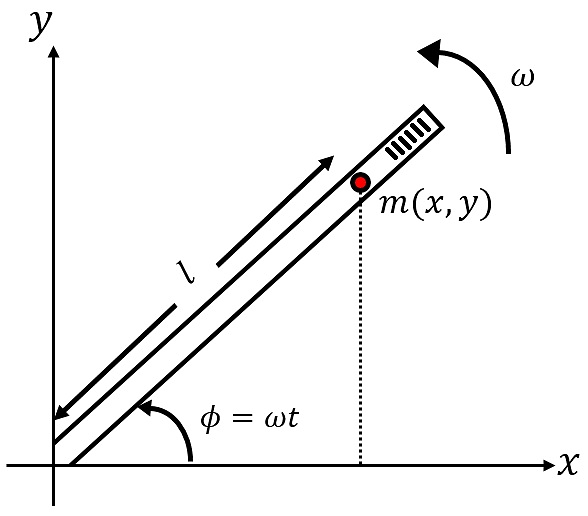
\includegraphics[width=4.46875in,height=3.92156in]{Imagenes/media/image36.png}

Inicialmente es de tener en cuenta que no se trata de un sistema no
conservativo, por lo tanto se hace necesario utilizar la ecuación de
movimiento de Lagrange escrita en (57). De este modo, para obtener el
Lagrangiano, pártase de la energía cinética que está dada por:

\[T = \frac{1}{2}m\left( {\dot{x}}^{2} + {\dot{y}}^{2} \right)\]

Es conveniente manipular este problema en coordenadas polares; así,
haciendo las transformaciones correspondientes se tiene que:

\[\cos\phi = \frac{x}{l} \rightarrow x = l\cos\phi \rightarrow x = l\cos{\omega t}\]

\[{sen}\phi = \frac{y}{l} \rightarrow y = l{sen}\phi \rightarrow y = l{sen}{\omega t}\]

Por lo tanto:

\[\dot{x} = \dot{l}\cos{\omega t} - l\omega{sen}{\omega t} \rightarrow {\dot{x}}^{2} = {\dot{l}}^{2}\cos^{2}\omega t - 2\dot{l}l\omega\cos{\omega t}{sen}{\omega t} + l^{2}\omega^{2}{sen}^{2}\omega t\]

\[\dot{y} = \dot{l}{sen}{\omega t} + l\omega\cos{\omega t} \rightarrow {\dot{y}}^{2} = {\dot{l}}^{2}{sen}^{2}\omega t + 2\dot{l}l\omega{sen}{\omega t}\cos{\omega t} + l^{2}\omega^{2}\cos^{2}\omega t\]

\[{\dot{x}}^{2} + {\dot{y}}^{2} = {\dot{l}}^{2} + l^{2}\omega^{2}\]

De esta forma, la energía cinética está dada por:

\[T = \frac{1}{2}m\left( {\dot{l}}^{2} + l^{2}\omega^{2} \right)\]

Por otro lado, la energía potencial es:

\[U = mgy \rightarrow U = mgl{sen}{\omega t}\]

Por lo tanto, el Lagrangiano del sistema es:

\[L = \frac{1}{2}m\left( {\dot{l}}^{2} + l^{2}\omega^{2} \right) - mgl{sen}{\omega t}\]

Las derivadas correspondientes para llevar a la ecuación de movimiento
de Lagrange son:

\[\frac{\partial L}{\partial\dot{l}} = m\dot{l},\ \ \ \ \ \ \ \ \ \ \frac{\partial L}{\partial l} = ml\omega^{2} - mg{sen}{\omega t}\]

Así:

\[\frac{d}{dt}\left( m\dot{l} \right) - ml\omega^{2} + mg{sen}{\omega t} = 0\]

\[m\ddot{l} - ml\omega^{2} + mg{sen}{\omega t} = 0\]

Luego; la ecuación de movimiento es:

\[\ddot{\mathbf{l}}\mathbf{- l}\mathbf{\omega}^{\mathbf{2}}\mathbf{= - g}\mathbf{sen}\mathbf{\omega t}\]

Nótese que el término de la derecha de la igualdad es una fuerza de
giro, se tiene una ecuación diferencial de segundo orden no homogénea
que la solución va a estar dada por:

\[l(t) = l_{h} + l_{p}\]

Donde, la solución homogénea \(l_{h}\) es:

\[l_{h} = A_{1}e^{\omega t} + A_{2}e^{- \omega t}\]

Y la solución particular \(l_{p}\) es:

\[l_{p} = \frac{g}{2\omega^{2}}{sen}{\omega t}\]

Finalmente, la solución general de la ecuación de movimiento de Lagrange
obtenida para este caso es:

\[\mathbf{l}\left( \mathbf{t} \right)\mathbf{=}\mathbf{A}_{\mathbf{1}}\mathbf{e}^{\mathbf{\omega t}}\mathbf{+}\mathbf{A}_{\mathbf{2}}\mathbf{e}^{\mathbf{- \omega t}}\mathbf{+}\frac{\mathbf{g}}{\mathbf{2}\mathbf{\omega}^{\mathbf{2}}}\mathbf{sen}\mathbf{\omega t}\]

\textbf{Ejemplo 6:} Encontrar la ecuación de movimiento del sistema
indicado en la \emph{figura 21}, bajo el supuesto de que \((x - a)\) es
la deformación del primer resorte en estado de compresión y \((x + b)\)
es la deformación en estado de estiramiento. Si se consideran pequeñas
oscilaciones \(\phi \ll 1\), además \(k_{1} = k_{2}\). Demostrar que:

\[\omega^{2} = \frac{2kl + mg}{ml}\]

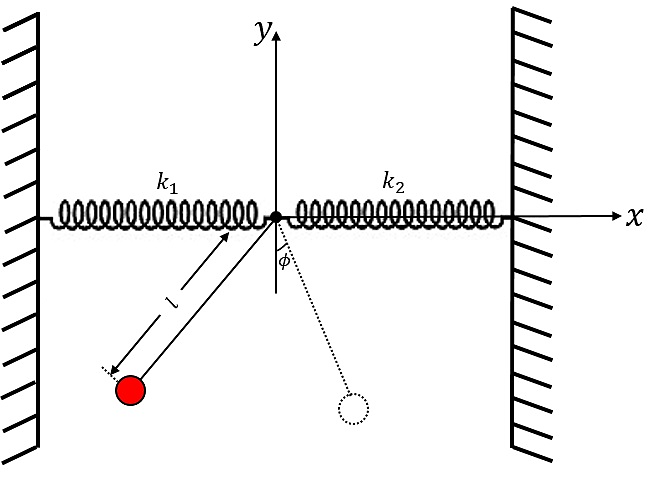
\includegraphics[width=5.05208in,height=3.5in]{Imagenes/media/image37.png}

\textbf{Solución:} Inicialmente es de considerar que como se trata de un
sistema que no es conservativo se hace necesario usar la ecuación de
movimiento de Lagrange generalizada, además es conveniente hacer una
descripción de la situación mediante coordenadas polares, por lo tanto:

\[{sen}\phi = \frac{x}{l} \rightarrow x = l{sen}\phi\]

\[\cos\phi = \frac{y}{l} \rightarrow y = l\cos\phi\]

Como la energía cinética está dada por:

\[T = \frac{1}{2}m\left( {\dot{x}}^{2} + {\dot{y}}^{2} \right)\]

Así:

\[\dot{x} = l\dot{\phi}\cos\phi \rightarrow {\dot{x}}^{2} = l^{2}{{\dot{\phi}}^{2}\cos}^{2}\phi\]

\[\dot{y} = - l\dot{\phi}{sen}\phi \rightarrow {\dot{y}}^{2} = l^{2}{{\dot{\phi}}^{2}sen}^{2}\phi\]

\[{\dot{x}}^{2} + {\dot{y}}^{2} = l^{2}{\dot{\phi}}^{2}\]

Luego, la energía cinética es:

\[T = \frac{1}{2}ml^{2}{\dot{\phi}}^{2}\]

Para este caso; se tiene para la energía potencial que
\(k_{1} = k_{2} = k\) y se puede escribir como:

\[U = \frac{1}{2}k{(x - a)\ }^{2} + \frac{1}{2}k{(x + b)\ }^{2} - mgy\]

\[U = \frac{1}{2}k{(l{sen}\phi - a)\ }^{2} + \frac{1}{2}k{(l{sen}\phi + b)\ }^{2} - mgl\cos\phi\]

Luego; el Lagrangiano de este sistema es:

\[L = \frac{1}{2}ml^{2}{\dot{\phi}}^{2} - \frac{1}{2}k\left( l{sen}\phi - a \right)^{2} - \frac{1}{2}k\left( l{sen}\phi + b \right)^{2} + mgl\cos\phi\]

Las derivadas correspondientes para llevar a la ecuación de movimiento
de Lagrange son:

\[\frac{\partial L}{\partial\dot{\phi}} = ml^{2}\dot{\phi},\ \ \ \ \ \ \ \ \ \ \frac{\partial L}{\partial\phi} = - k\left( l{sen}\phi - a \right)l\cos\phi - k\left( l{sen}\phi + b \right)l\cos\phi - mgl{sen}\phi\]

De esta manera la ecuación de movimiento asociada al sistema es:

Como para ángulos \(\phi\) pequeños \({sen}\phi \approx \phi\) y
\(\cos\phi \approx 1\), entonces:

\[ml^{2}\ddot{\phi} + kl^{2}\phi - kal + kl^{2}\phi + kbl + mgl\phi = 0\]

\[ml^{2}\ddot{\phi} + \left( 2kl^{2} + mgl \right)\phi + kl(b - a) = 0\]

\[\ddot{\phi} + \frac{(2kl + mg)}{ml}\phi + \frac{k}{ml}(b - a) = 0\]

Nótese que la expresión anterior corresponde al modelo de un MAS tal
como era de esperarse donde la fuerza de restitución elástica está dada
por:

Reescribiendo la ecuación de movimiento se tiene:

\[\ddot{\phi} + \omega^{2}\phi = \frac{k}{ml}(a - b)\]

\[\mathbf{\omega}^{\mathbf{2}}\mathbf{=}\frac{\mathbf{2}\mathbf{kl + mg}}{\mathbf{ml}}\]

Cuya solución es:

\[\mathbf{\phi}\left( \mathbf{t} \right)\mathbf{= A + C}\mathbf{sen}\left( \mathbf{\omega t + \phi} \right)\]

\textbf{PRINCIPIO DE MÍNIMA ACCIÓN}

En sistemas de la mecánica clásica, el principio de mínima acción
postulaba que la evolución temporal de cualquier sistema físico estaba
dado por la tendencia a mínimo que tenía una magnitud llamada
``acción''.

Años después se logró obtener una generalización de este principio a
sistemas continuos donde ya las magnitudes básicas dependían de las
coordenadas espacio\(-\)temporales y no únicamente de una sola variable
temporal. Por otro lado cuando se logró la formulación relativista del
principio, se trajo consigo una prueba de que tener una condición de
mínimo implicaba grandes restricciones por lo que debía ser reemplazada
por la condición un poco más general de que la trayectoria debía ser un
punto crítico o estacionario, un mínimo o un máximo pero no un valor no
extremal si se habla en términos de cálculo variacional.

Pierre\(-\)Louis Moreau de Maupertuis fue quien estableció la primera
formulación de este principio, en 1744 Moreau manifestó que la
``naturaleza es económica en todas sus acciones''. Años antes, Pierre de
Fermat había dado una idea de que los rayos de luz, en situaciones de
óptica geométrica cumplían con una trayectoria en la cual el tiempo era
mínimo tal como se establece en el principio de Fermat. Desde el punto
de vista del cálculo variacional es más preciso hablar del principio de
mínima acción estacionario. Dentro de quiénes desarrollaron la idea se
incluyen Euler y Leibniz.

A partir del principio de mínima acción se dio dirección al desarrollo
de las formulaciones del Lagrangiano y el Hamiltoniano dados en la
mecánica clásica.

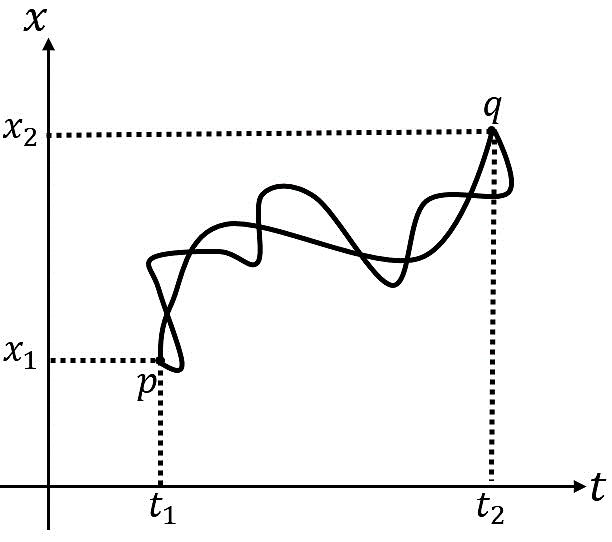
\includegraphics[width=4.17708in,height=3.69931in]{Imagenes/media/image38.png}El
principio de mínima acción es un principio integral que permite obtener
la curva que realmente describe un sistema y se busca conocer cómo
evoluciona el Lagrangiano en un intervalo
\(\left\lbrack t_{1},\ t_{2} \right\rbrack\) para que la partícula vaya
de \(p\) a \(q\).

La formulación de acción está dada por:

\[S\left\lbrack x(t) \right\rbrack = \int_{t_{1}}^{t_{2}}{L\left( x,\dot{x};t \right)dt}\]

Los límites de integración son fijos y la familia de curvas próximas a
la curva real cumplen con las mismas condiciones físicas iniciales, es
decir, deben pasar por los puntos \(p\) y \(q\). Es necesario
parametrizar la función \(x(t)\), mediante un parámetro diferencial
pequeño se tiene:

\[x(t,\ \alpha) = x(t,0) + \alpha\eta(t)\]

\(\eta(t)\) es cualquier tipo de función que requiere que:

\begin{enumerate}
\def\labelenumi{\arabic{enumi})}
\item
  Sea una función continua.
\item
  \(\eta(t_{1}) = \ \eta\left( t_{2} \right) = 0\) para que toda la
  familia de curvas que pasen por \(p\) y \(q\) tengan las mismas
  condiciones físicas.
\end{enumerate}

Luego:

\[x(t,\ \alpha) - x(t,\ 0) = \alpha\eta(t)\]

Donde se hace necesario reescribir la acción como:

\[S\left\lbrack x(t,\alpha) \right\rbrack = \int_{t_{1}}^{t_{2}}{L\left\lbrack \left( x(t,\alpha),\dot{x}(t,\alpha);\ t \right) \right\rbrack dt}\]

Para encontrar la curva crítica se debe cumplir la condición de que:

\[\left. \ \frac{\partial S\left\lbrack x(t,\alpha) \right\rbrack}{\partial\alpha}d\alpha \right\rfloor_{\alpha = 0} = 0\]

De toda la familia de curvas o posibilidades que hay para ir del punto
\(p\) al punto \(q\) la que realmente sigue el sistema es aquella donde
la acción sea un mínimo, esto si se habla físicamente, en matemáticas se
hace referencia a una extremal. Por lo tanto:

\[\left. \ \frac{\partial S}{\partial\alpha}d\alpha \right\rfloor_{\alpha = 0} = \frac{\partial}{\partial\alpha}\int_{t_{1}}^{t_{2}}{L\left\lbrack \left( x(t,\alpha),\dot{x}(t,\alpha);\ t \right) \right\rbrack d\alpha\ dt} = 0\]

\[\left. \ \frac{\partial S}{\partial\alpha}d\alpha \right\rfloor_{\alpha = 0} = \int_{t_{1}}^{t_{2}}\left( \frac{\partial L}{\partial x}\frac{\partial x(t,\ \alpha)}{\partial\alpha} + \frac{\partial L}{\partial\dot{x}}\frac{\partial\dot{x}(t,\ \alpha)}{\partial\alpha} \right)d\alpha\ dt = 0\]

Como:

\[x(t,\ \alpha) = x(t,0) + \alpha\eta(t)\ \ \ \ \ \ \ y\ \ \ \ \ \ \ \frac{\partial x}{\partial\alpha} = \eta(t)\]

Entonces:

\[\dot{x}(t,\ \alpha) = \dot{x}(t,\ o) + \alpha\frac{d\eta}{dt} = \dot{x}(t,\ o) + \alpha\dot{\eta}(t)\]

Además:

\[\frac{\partial\dot{x}(t,\ \alpha)}{\partial\alpha} = \dot{\eta}(t) = \frac{d\eta(t)}{dt}\]

De este modo:

\[\int_{t_{1}}^{t_{2}}{\left\lbrack \frac{\partial L}{\partial x}\eta(t) + \frac{\partial L}{\partial\dot{x}}\frac{d\eta}{dt} \right\rbrack_{\alpha = 0}d\alpha\ dt = 0}\]

Tomando el segundo término de la integral y reescribiéndolo se tiene
que:

\[\frac{\partial L}{\partial\dot{x}}\frac{d\eta}{dt} \rightarrow \frac{d}{dt}\left\lbrack \frac{\partial L}{\partial\dot{x}}\eta(t) \right\rbrack\]

\[\frac{d}{dt}\left\lbrack \frac{\partial L}{\partial\dot{x}}\eta(t) \right\rbrack = \frac{d}{dt}\frac{\partial L}{\partial\dot{x}}\eta(t) + \frac{\partial L}{\partial\dot{x}}\frac{d\eta}{dt}\]

\[\frac{\partial L}{\partial\dot{x}}\frac{d\eta}{dt} = \frac{d}{dt}\left\lbrack \frac{\partial L}{\partial\dot{x}}\eta(t) \right\rbrack - \frac{d}{dt}\frac{\partial L}{\partial\dot{x}}\eta(t)\]

Luego, reescribiendo la integral (77) se da que:

\[\int_{t_{1}}^{t_{2}}{\left\lbrack \frac{\partial L}{\partial x}\eta(t) - \frac{d}{dt}\frac{\partial L}{\partial\dot{x}}\eta(t) \right\rbrack d\alpha\ dt\  + \ \int_{t_{1}}^{t_{2}}{\frac{d}{dt}\left\lbrack \frac{\partial L}{\partial\dot{x}}\eta(t) \right\rbrack d\alpha\ dt} = 0}\]

\[\int_{t_{1}}^{t_{2}}{\left\lbrack \frac{\partial L}{\partial x} - \frac{d}{dt}\frac{\partial L}{\partial\dot{x}} \right\rbrack d\alpha\ \eta(t)\ dt\  + \ \int_{t_{1}}^{t_{2}}{\frac{d}{dt}\left\lbrack \frac{\partial L}{\partial\dot{x}}\eta(t) \right\rbrack d\alpha\ dt} = 0}\]

La segunda integral se hace cero, por lo tanto:

\[\eta(t_{1}) = \ \eta\left( t_{2} \right) = 0\]

y también:

\[\left. \ \frac{\partial L}{\partial\dot{x}}\eta(t) \right\rfloor_{t_{1}}^{t_{2}} = \frac{\partial L}{\partial\dot{x}}\eta\left( t_{2} \right) - \frac{\partial L}{\partial\dot{x}}\eta\left( t_{1} \right) = 0\]

Además:

\[\int_{t_{1}}^{t_{2}}{\left\lbrack \frac{\partial L}{\partial x} - \frac{d}{dt}\frac{\partial L}{\partial\dot{x}} \right\rbrack d\alpha\ \eta(t)\ dt\  = 0}\]

, entonces se puede escribir la ecuación de movimiento de Lagrange a
partir del principio de mínima acción:

\[\frac{\partial L}{\partial x} - \frac{d}{dt}\frac{\partial L}{\partial\dot{x}} = 0\]

\[\frac{\mathbf{d}}{\mathbf{dt}}\frac{\mathbf{\partial L}}{\mathbf{\partial}\dot{\mathbf{x}}}\mathbf{-}\frac{\mathbf{\partial L}}{\mathbf{\partial x}}\mathbf{= 0}\]

Ahora, considerando una partícula moviéndose en una dirección bajo la
acción de un potencial \(U(x)\), se tiene:

\[S = \int_{t_{1}}^{t_{2}}{L\left( x,\dot{x},t \right)dt}\]

\[S\left\lbrack x(t) \right\rbrack = \int_{t_{1}}^{t_{2}}{\left( \frac{1}{2}m\left\lbrack \frac{d}{dt}x(t) \right\rbrack^{2} - U(x) \right)dt}\]

Introduciendo el parámetro diferencial \(\alpha\) la expresión toma la
forma:

\[S\left\lbrack x(t,\alpha) \right\rbrack = \int_{t_{1}}^{t_{2}}{\left( \frac{1}{2}m\left\lbrack \frac{d}{dt}x(t,\alpha) \right\rbrack^{2} - U\lbrack x(t,\alpha)\rbrack \right)dt}\]

Como \(x(t,\ \alpha) = x(t,0) + \alpha\eta(t)\) además teniendo en
cuenta la condición de mínimo escrita en (76) se cumple que:

\[\left. \ \frac{\partial S}{\partial\alpha}d\alpha \right\rfloor_{\alpha = 0} = \frac{\partial}{\partial\alpha}\int_{t_{1}}^{t_{2}}{\left( \frac{1}{2}m\left\lbrack \frac{d}{dt}(x(t,0) + \alpha\eta(t)) \right\rbrack^{2} - U\lbrack x(t,0) + \alpha\eta(t)\rbrack \right)d\alpha\ dt} = 0\]

\[\left. \ \frac{\partial S}{\partial\alpha}d\alpha \right\rfloor_{\alpha = 0} = \int_{t_{1}}^{t_{2}}\left\lbrack m\frac{dx(t,0)}{dt}\frac{d\eta}{dt} - \frac{\partial U}{\partial x}\eta(t) \right\rbrack d\alpha\ dt = 0\]

\[\int_{t_{1}}^{t_{2}}m\frac{dx(t,0)}{dt}\frac{d\eta}{dt}\ dt\]

Haciendo integración por partes; sean:

\[u = \frac{mdx(t,0)}{dt},\ \ \ \ \ \ dv = \frac{d\eta}{dt}\ dt,\ \ \ \ \ \ v = \eta(t)\ \ \ \ \ \ y\ \ \ \ \ \ du = m\frac{d^{2}x(t,0)}{dt^{2}}dt\]

De esta manera:

\[\int_{t_{1}}^{t_{2}}m\frac{dx(t,0)}{dt}\frac{d\eta}{dt}\ dt = \left. \ m\frac{dx(t,0)}{dt}\eta(t) \right\rfloor_{t_{1}}^{t_{2}} - \int_{t_{1}}^{t_{2}}{m\frac{d^{2}x(t,0)}{dt^{2}}\eta(t)dt}\]

\[- \int_{t_{1}}^{t_{2}}{\left\lbrack m\frac{d^{2}x(t,0)}{dt^{2}} + \frac{\partial U}{\partial x} \right\rbrack da\ \eta(t)\ dt = 0}\]

Finalmente;

\[\mathbf{m}\frac{\mathbf{d}^{\mathbf{2}}\mathbf{x}\left( \mathbf{t,0} \right)}{\mathbf{d}\mathbf{t}^{\mathbf{2}}}\mathbf{+}\frac{\mathbf{\partial U}}{\mathbf{\partial x}}\mathbf{= 0}\]

\[\mathbf{m}\frac{\mathbf{d}^{\mathbf{2}}\mathbf{x}\left( \mathbf{t,0} \right)}{\mathbf{d}\mathbf{t}^{\mathbf{2}}}\mathbf{= -}\frac{\mathbf{\partial U}}{\mathbf{\partial x}}\]

La expresión (78) corresponde a la equivalencia entre la segunda Ley de
Newton y el principio de mínima acción.

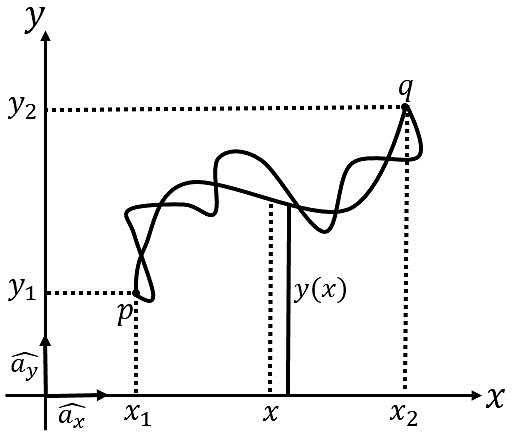
\includegraphics[width=4.65625in,height=4.01965in]{Imagenes/media/image39.png}Análogamente
se puede hacer una descripción de, principio en términos matemáticos,
para esto se considera la \emph{figura 23}:

Se define la acción como:

\[J\left\lbrack y(x) \right\rbrack = \int_{x_{1}}^{x_{2}}{f\left\lbrack y(x),\ \dot{y}(x);x \right\rbrack dx}\]

Se pretende buscar que \(y(x)\) tome un valor extremal.

\[y(x) + \delta y = y_{\nu}\]

\(y_{\nu}\) corresponde a toda la familia de curvas, introduciendo ahora
el parámetro pequeño diferencial se tiene que:

\[y_{\nu}(x,\ \alpha) = y(x,\ 0) + \alpha\eta(x)\]

\(\eta(x)\) es cualquier tipo de función continua. Así:

\[J\left\lbrack y(x,\ \alpha) \right\rbrack = \int_{x_{1}}^{x_{2}}{f\left\lbrack y(x,\ \alpha),\ \dot{y}(x,\alpha);x \right\rbrack dx}\]

Para encontrar la función se hace que \(J\) tome un valor extremal, por
lo que:

\[\left. \ \frac{\partial J\left\lbrack y(x,\alpha) \right\rbrack}{\partial\alpha}d\alpha \right\rfloor_{\alpha = 0} = 0\]

La expresión (80) da la condición para tener una curva extremal. \(f\)
recibe el nombre de funcional. De este modo:

\[\frac{\partial}{\partial\alpha}\int_{x_{1}}^{x_{2}}{f\left\lbrack y(x,\ \alpha),\ \dot{y}(x,\alpha);x \right\rbrack d\alpha\ dx = 0}\]

\[\int_{x_{1}}^{x_{2}}{\left( \frac{\partial f}{\partial y}\frac{\partial y}{\partial\alpha} + \frac{\partial f}{\partial\dot{y}}\frac{\partial\dot{y}}{\partial\alpha} \right)d\alpha\ dx = 0}\]

Como:

\[\frac{\partial y}{\partial\alpha} = \eta(x)\]

Entonces:

\[\int_{x_{1}}^{x_{2}}{\left( \frac{\partial f}{\partial y}\eta(x) + \frac{\partial f}{\partial\dot{y}}\frac{d\eta}{dx} \right)d\alpha\ dx = 0}\]

\[\frac{\partial f}{\partial\dot{y}}\frac{d\eta}{dx} \rightarrow \frac{d}{dx}\left\lbrack \frac{\partial f}{\partial\dot{y}}\eta(x) \right\rbrack = \frac{d}{dx}\frac{\partial f}{\partial\dot{y}}\eta(x) + \frac{\partial f}{\partial\dot{y}}\frac{d\eta}{dx} \rightarrow\]

\[\frac{\partial f}{\partial\dot{y}}\frac{d\eta}{dx} = \frac{d}{dx}\left\lbrack \frac{\partial f}{\partial\dot{y}}\eta(x) \right\rbrack - \frac{d}{dx}\frac{\partial f}{\partial\dot{y}}\eta(x)\]

Luego, reescribiendo la integral (81) se da que:

\[\int_{x_{1}}^{x_{2}}{\left\lbrack \frac{\partial f}{\partial y}\eta(x) - \frac{d}{dx}\frac{\partial f}{\partial\dot{y}}\eta(x) \right\rbrack d\alpha\ dx\  + \ \int_{x_{1}}^{x_{2}}{\frac{d}{dx}\left\lbrack \frac{\partial f}{\partial\dot{y}}\eta(x) \right\rbrack d\alpha\ dx} = 0}\]

\[\int_{t_{1}}^{t_{2}}{\left\lbrack \frac{\partial L}{\partial x} - \frac{d}{dt}\frac{\partial L}{\partial\dot{x}} \right\rbrack d\alpha\ \eta(x)\ dt\  = 0}\]

La segunda integral se hace cero, por lo tanto:

\[\eta(x_{1}) = \ \eta\left( x_{2} \right) = 0\]

y también:

\[\left. \ \frac{\partial f}{\partial\dot{y}}\eta(x) \right\rfloor_{x_{1}}^{x_{2}} = \frac{\partial f}{\partial\dot{y}}\eta\left( x_{2} \right) - \frac{\partial L}{\partial\dot{f}}\eta\left( x_{1} \right) = 0\]

Además:

\[\int_{x_{1}}^{x_{2}}{\left\lbrack \frac{\partial f}{\partial y} - \frac{d}{dx}\frac{\partial f}{\partial\dot{y}} \right\rbrack d\alpha\ \eta(t)\ dt\  = 0}\]

Como \(d\alpha\ \eta(x)dx = J\left\lbrack y(x,\ \alpha) \right\rbrack\),
entonces:

\[\frac{\mathbf{\partial f}}{\mathbf{\partial y}}\mathbf{-}\frac{\mathbf{d}}{\mathbf{dx}}\frac{\mathbf{\partial f}}{\mathbf{\partial}\dot{\mathbf{y}}}\mathbf{= 0}\]

La ecuación (82) corresponde a la ecuación de Euler y es una analogía en
términos matemáticos que recibe la ecuación de movimiento de Lagrange.

Por otro lado, al buscar una generalización de lo anteriormente descrito
se va a tener que:

\[J\left\lbrack y_{i}(x) \right\rbrack = \int_{x_{1}}^{x_{2}}{f\left\lbrack y_{1}(x),\ y_{2}(x),\ldots,y_{i}(x),{\dot{y}}_{1}(x),\ {\dot{y}}_{2}(x),\ldots,{\dot{y}}_{i}(x);x \right\rbrack dx}\]

De esta manera:

\[\eta_{1}\left( x_{1} \right) = \eta_{1}\left( x_{2} \right)\]

\[\eta_{i}\left( x_{1} \right) = \eta_{i}\left( x_{2} \right)\]

Además con el parámetro diferencial \(\alpha\),\({\ y}_{i}\) toma la
forma:

\[y_{1}(x,\ \alpha) = y_{1}(x,\ 0) + \alpha\eta_{1}(x)\]

\[{y_{2}(x,\ \alpha) = y_{2}(x,\ 0) + \alpha\eta_{2}(x)
}{\ \ \ \ \ \ .\ \ \ \ \ \ \ \ \ \ \ \ \ \ \ \ \ \ \ .\ \ \ \ \ \ \ \ \ \ \ \ \ \ \ \ \ \ \ .
}{\ \ \ \ \ \ .\ \ \ \ \ \ \ \ \ \ \ \ \ \ \ \ \ \ \ .\ \ \ \ \ \ \ \ \ \ \ \ \ \ \ \ \ \ \ .
}{\ \ \ \ \ \ .\ \ \ \ \ \ \ \ \ \ \ \ \ \ \ \ \ \ \ .\ \ \ \ \ \ \ \ \ \ \ \ \ \ \ \ \ \ \ .
}{\ y_{i}(x,\ \alpha) = y_{i}(x,\ 0) + \alpha\eta_{i}(x)}\]

La condición de extremal va a estar determinada por:\(\ \ \)

\[\left. \ \frac{\partial J\left\lbrack y_{i}(x,\alpha) \right\rbrack}{\partial\alpha}d\alpha \right\rfloor_{\alpha = 0} = 0\]

De este modo:

\[J\left\lbrack y_{i}(x,\alpha) \right\rbrack = \int_{x_{1}}^{x_{2}}{f\left\lbrack y_{i}(x,\ \alpha),{\dot{y}}_{i}(x,\alpha);x \right\rbrack dx}\]

\[\left. \ \frac{\partial J}{\partial\alpha}d\alpha \right\rfloor_{\alpha = 0} = 0 = \frac{\partial}{\partial\alpha}\int_{x_{1}}^{x_{2}}{f\left\lbrack y_{i}(x,\ \alpha),{\dot{y}}_{i}(x,\alpha);x \right\rbrack d\alpha\ dx}\]

\[\int_{x_{1}}^{x_{2}}{\sum_{i}^{}{\left( \frac{\partial f}{\partial y_{i}}\frac{\partial y_{i}}{\partial\alpha} + \frac{\partial f}{\partial{\dot{y}}_{i}}\frac{\partial{\dot{y}}_{i}}{\partial\alpha} \right)d\alpha\ dx} = 0}\]

Como:

\[\frac{\partial y_{i}}{\partial\alpha} = \eta_{i}(x)\]

Luego:

\[\int_{x_{1}}^{x_{2}}{\sum_{i}^{}{\left( \frac{\partial f}{\partial y_{i}}\frac{\partial y_{i}}{\partial\alpha} + \frac{\partial f}{\partial{\dot{y}}_{i}}\frac{\partial{\dot{y}}_{i}}{\partial\alpha} \right)d\alpha\ dx} =}\int_{x_{1}}^{x_{2}}{\sum_{i}^{}{\left( \frac{\partial f}{\partial y_{i}}\eta_{i}(x) + \frac{\partial f}{\partial{\dot{y}}_{i}}\dot{\eta_{i}}(x) \right)d\alpha\ dx}} = 0\]

\[\sum_{i}^{}{\frac{\partial f}{\partial{\dot{y}}_{i}}\dot{\eta_{i}}(x)} \rightarrow \sum_{i}^{}{\frac{d}{dx}\left\lbrack \frac{\partial f}{\partial{\dot{y}}_{i}}\eta_{i}(x) \right\rbrack} = \sum_{i}^{}{\frac{d}{dx}\frac{\partial f}{\partial{\dot{y}}_{i}}\eta_{i}(x) + \frac{\partial f}{\partial{\dot{y}}_{i}}\frac{d\eta_{i}(x)}{dx}}\]

Luego, la integral (84) se puede escribir como:

\[\int_{x_{1}}^{x_{2}}{\sum_{i}^{}{\left\lbrack \frac{\partial f}{\partial y_{i}} - \frac{d}{dx}\frac{\partial f}{\partial{\dot{y}}_{i}} \right\rbrack\eta_{i}(x)d\alpha\ dx}\  + \ \int_{x_{1}}^{x_{2}}{\frac{d}{dx}\left\lbrack \frac{\partial f}{\partial{\dot{y}}_{i}}\eta_{i}(x) \right\rbrack d\alpha\ dx} = 0}\]

Finalmente:

\[\frac{\partial f}{\partial y_{i}} - \frac{d}{dx}\frac{\partial f}{\partial{\dot{y}}_{i}} = 0\]

Ecuación de Euler-Lagrange

En este orden de ideas el Lagrangiano queda escrito de la siguiente
forma:

\[L = L(q_{1},\ q_{2},\ q_{3},\ldots,\ q_{i},\ \dot{q_{1}},\ \dot{q_{2}},\ \dot{q_{3}},\ldots,\dot{q_{i}};t)\]

Las \(n\) coordenadas generalizadas forman un nuevo espacio que no es el
real al cual se le da el nombre de \emph{hiperespacio.}

\[\frac{\partial L}{\partial q_{i}} - \frac{d}{dt}\frac{\partial L}{\partial\dot{q_{i}}} = 0\]

Ecuación de movimiento de Lagrange

Un punto en el hiperespacio puede corresponder al estado de un sistema,
si se habla de termodinámica, por ejemplo.

El cambio de la trayectoria en el hiperespacio corresponde a la
evolución de los estados del sistema, está claro que no es la
trayectoria real.

\textbf{Ejemplo 7:} Sea la curva mostrada en la \emph{figura 24}. Hallar
la ecuación de la curva más corta que pasa por los puntos
\(P_{1}(x_{1},y_{1})\) y \(P_{2}(x_{2},y_{2})\).

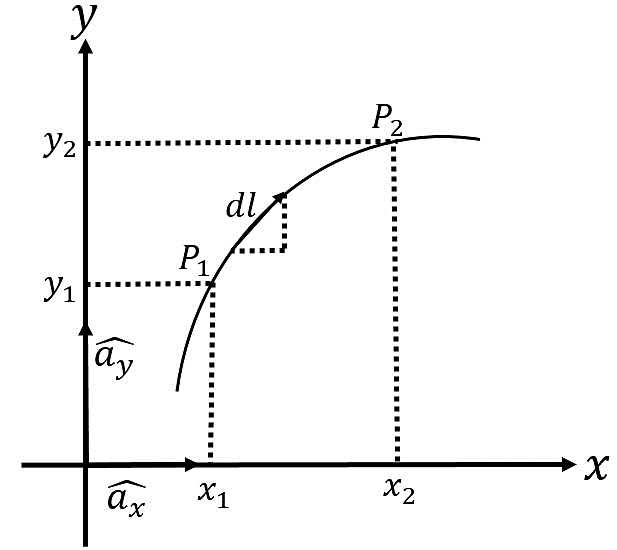
\includegraphics[width=4.73958in,height=4.225in]{Imagenes/media/image40.png}

\textbf{Solución:} Inicialmente es necesario escribir la integral que
hay que resolver, de esta manera:

\[d\overrightarrow{l} = dx\widehat{a_{x}} + dy\widehat{a_{y}}\]

\[\left| d\overrightarrow{l} \right| = dl = \sqrt{{(dx)}^{2} + {(dy)}^{2}}\]

Reescribiendo:

\[dl = \sqrt{{(dx)}^{2}\left( 1 + \left( \frac{dy}{dx} \right)^{2} \right)^{}}\]

\[dl = \sqrt{1 + {\dot{y}}^{2}}dx\]

Por el principio de mínima acción:

\[l = \int_{x_{1}}^{x_{2}}{\sqrt{1 + {\dot{y}}^{2}}dx}\]

Es de notar que \(l\) es el extremal, \(\sqrt{1 + {\dot{y}}^{2}}\) la
funcional y \(dx\) es el parámetro, luego:

Usando la ecuación de Euler:

\[f = \sqrt{1 + {\dot{y}}^{2}}\]

\[\frac{\partial f}{\partial\dot{y}} = \frac{\dot{y}}{\sqrt{1 + {\dot{y}}^{2}}}\]

\[\frac{\partial f}{\partial y} = 0\]

De esta manera:

\[\frac{d}{dx}\left( \frac{\dot{y}}{\sqrt{1 + {\dot{y}}^{2}}} \right) - \frac{\partial f}{\partial y} = 0\]

\[\frac{d}{dx}\left( \frac{\dot{y}}{\sqrt{1 + {\dot{y}}^{2}}} \right) = 0\]

Para que la igualdad se cumpla lo que se encuentra dentro del paréntesis
debe ser una constante, de esta manera:

\[\frac{\dot{y}}{\sqrt{1 + {\dot{y}}^{2}}} = A\]

Por lo tanto:

\[\dot{y} = A\sqrt{1 + {\dot{y}}^{2}}\]

\[{\dot{y}}^{2} = A^{2}\left( 1 + {\dot{y}}^{2} \right)\]

Reescribiendo:

\[{\dot{y}}^{2}\left( 1 - A^{2} \right) = A^{2}\]

\[\dot{y} = \frac{A}{\sqrt{1 - A^{2}}}\]

\[\frac{dy}{dx} = \frac{A}{\sqrt{1 - A^{2}}}\]

Luego la integral a resolver es:

\[\int_{}^{}{dy} = \int_{}^{}adx\]

\(\mathbf{y = ax + b}\) \textbf{ecuación general}

Finalmente se concluye que la ecuación de la curva más corta que pasa
por los puntos \(P_{1}(x_{1},y_{1})\) y \(P_{2}(x_{2},y_{2})\) es la
ecuación de una línea recta donde \(a\) y \(b\) se encuentran con las
condiciones de frontera.

\textbf{Ejemplo 8:} Considerar una superficie de revolución generada por
el giro de una curva \(y(x)\) alrededor del eje \(y\), se requiere que
la curva pase a través de puntos extremos fijos \((x_{1},y_{1})\) y
\((x_{2},y_{2})\). El problema variacional consiste en seleccionar la
curva \(y = y(x)\) de modo que el área de la superficie resultante sea
mínima.

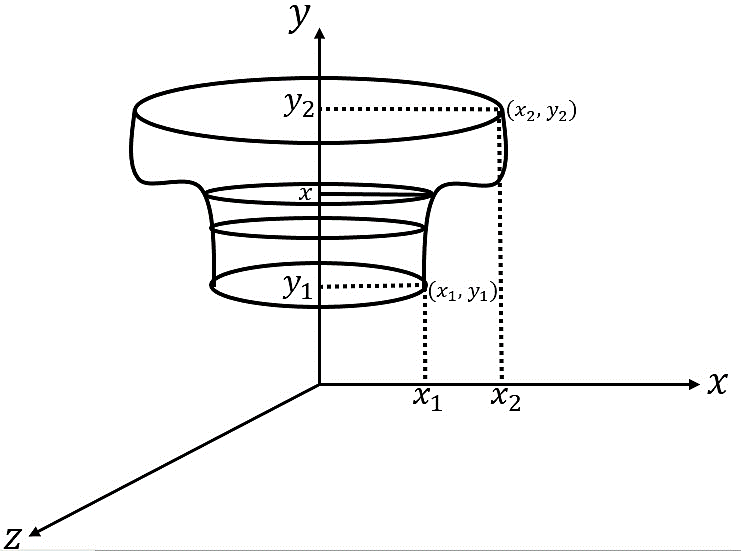
\includegraphics[width=6.08611in,height=4.51042in]{Imagenes/media/image41.png}\textbf{Solución:}
Considérese la siguiente superficie de revolución:

Como se busca el área mínima; se define un diferencial de área con \(x\)
y \(d\overrightarrow{l},\ \)de esta manera:

\[dA = 2\pi xdl\]

Obteniendo la norma de \(d\overrightarrow{l}\), se tiene:

\[d\overrightarrow{l} = dx\widehat{a_{x}} + dy\widehat{a_{y}}\]

\[\left| d\overrightarrow{l} \right| = dl = \sqrt{{(dx)}^{2} + {(dy)}^{2}}\]

\[dl = \sqrt{{(dx)}^{2}\left( 1 + \left( \frac{dy}{dx} \right)^{2} \right)^{}}\]

\[dl = \sqrt{1 + {\dot{y}}^{2}}dx\]

Por lo tanto:

\[dA = 2\pi x\sqrt{1 + {\dot{y}}^{2}}dx\]

\[A = \int_{x_{1}}^{x_{2}}{2\pi x\sqrt{1 + {\dot{y}}^{2}}dx}\]

\[A = 2\pi\int_{x_{1}}^{x_{2}}{x\sqrt{1 + {\dot{y}}^{2}}dx}\]

Nótese que en este caso \(A\) es la cantidad que toma el extremal,
\(dx\) es un parámetro independiente y la funcional es
\(x\sqrt{1 + {\dot{y}}^{2}}dx\), de esta manera, usando la ecuación de
Euler se cumple que:

\[f = x\sqrt{1 + {\dot{y}}^{2}}\]

\[\frac{\partial f}{\partial\dot{y}} = \frac{x\dot{y}}{\sqrt{1 + {\dot{y}}^{2}}}\]

\[\frac{\partial f}{\partial y} = 0\]

De este modo:

\[\frac{d}{dx}\left( \frac{x\dot{y}}{\sqrt{1 + {\dot{y}}^{2}}} \right) = 0\]

Para que la igualdad se cumpla lo que se encuentra dentro del paréntesis
debe ser una constante, de esta manera:

\[\frac{x\dot{y}}{\sqrt{1 + {\dot{y}}^{2}}} = A\]

Así:

\[x\dot{y} = A\sqrt{1 + {\dot{y}}^{2}}\]

\[x^{2}{\dot{y}}^{2} = A^{2}\left( 1 + {\dot{y}}^{2} \right)\]

Reescribiendo:

\[x^{2}{\dot{y}}^{2} - A^{2}y^{2} = A^{2}\]

\[{\dot{y}}^{2}\left( x^{2} - A^{2} \right) = A^{2}\]

\[\dot{y} = \frac{A}{\sqrt{x^{2} - A^{2}}}\]

\[\frac{dy}{dx} = \frac{A}{\sqrt{x^{2} - A^{2}}}\]

Luego la integral que se hace necesario resolver es:

\[\int_{}^{}{dy} = \int_{}^{}\frac{A}{\sqrt{x^{2} - A^{2}}}dx\]

\[y = \int_{}^{}\frac{A}{\sqrt{x^{2} - A^{2}}}dx + B\]

Reescribiendo:

\[\frac{A}{\sqrt{x^{2} - A^{2}}} = \frac{A}{\sqrt{A^{2}\left( \frac{x^{2}}{A^{2}} - 1 \right)}}\]

De esta manera:

\[y = \int_{}^{}\frac{A}{\sqrt{A^{2}\left( \frac{x^{2}}{A^{2}} - 1 \right)}}dx + B\]

Esta integral tiene como solución:

\[y = Aarco\cosh\left( \frac{x}{A} \right) + B\]

\[y - B = Aarco\cosh\left( \frac{x}{A} \right)\]

\[\cosh\left( \frac{y - B}{A} \right) = \frac{x}{A}\]

\[\mathbf{x = A}\mathbf{\cosh}\left( \frac{\mathbf{y - B}}{\mathbf{A}} \right)\]

Por último es posible concluir que la curva \(y = y(x)\) que hacer que
el área de la superficie resultante sea mínima es una curva catenaria.

\textbf{PROBLEMA DE LA BRAQUISTÓCRONA}

El famoso problema de la braquistócrona ~pregunta qué forma debe tener
la trayectoria que sigue una partícula bajo la acción de la gravedad a
fin de minimizar el tiempo de descenso para descender desde un
punto~\(P_{1}(x_{1},y_{1})\) a un punto \(P_{2}(x_{2},y_{2})\). En junio
de 1696, Johann Bernoulli propuso este problema como un reto para la
comunidad científica, ofreciendo un plazo de seis meses (más tarde
extendido a la Pascua de 1697 a petición de George Leibniz). Isaac
Newton, entonces retirado de la vida académica y sirviendo como alcalde
de la Casa de Moneda en Londres, asumió el reto de Bernoulli el 29 de
enero de 1697. Al día siguiente comunicó su solución ---la curva de
descenso en el tiempo mínimo es un arco de cicloide invertida--- a la
Real Sociedad de Londres.~

Una curva
braquistócrona~(\href{https://es.wikipedia.org/wiki/Griego_antiguo}{gr.}
βραχίστος~brachistos~\textquotesingle el más corto\textquotesingle,
χρόνος~chronos~\textquotesingle{}\href{https://es.wikipedia.org/wiki/Intervalo}{intervalo}~de
tiempo\textquotesingle), o curva del descenso más rápido, es la curva
entre dos puntos que es recorrida en menor tiempo, por un cuerpo que
comienza en el punto inicial con velocidad cero, y que debe desplazarse
a lo largo de la curva hasta llegar al segundo punto, bajo acción de una
fuerza de
\href{https://es.wikipedia.org/wiki/Gravedad}{gravedad}~constante y
suponiendo que no
existe~\href{https://es.wikipedia.org/wiki/Fricci\%C3\%B3n}{fricción}.
En la solución del problema
intervinieron:~\href{https://es.wikipedia.org/wiki/Familia_Bernoulli}{Johann
y Jacobo Bernoulli},
\href{https://es.wikipedia.org/wiki/Leibniz}{Leibniz},~L\textquotesingle Hôpital,~\href{https://es.wikipedia.org/wiki/Isaac_Newton}{Newton},~Tschirnhaus,
entre otros. La solución de este problema dio origen al cálculo
variacional.

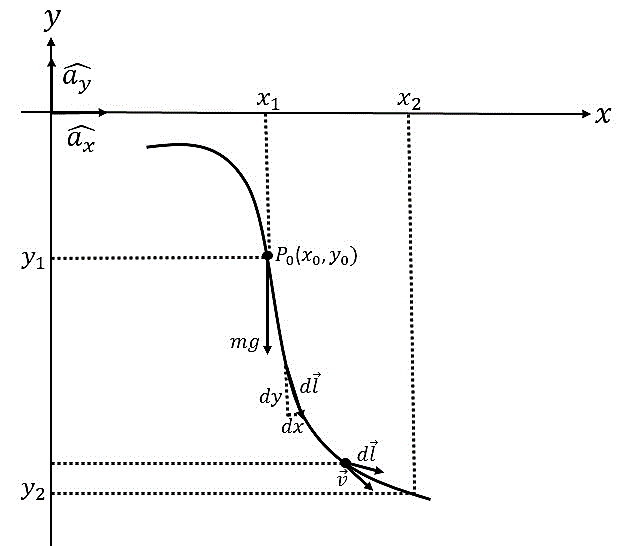
\includegraphics[width=5.15417in,height=4.41667in]{Imagenes/media/image42.png}Considérese
la situación mostrada en la \emph{figura 26:}

Se tiene que:

\[d\overrightarrow{l} = dx\widehat{a_{x}} - dy\widehat{a_{y}}\]

\[\left| d\overrightarrow{l} \right| = dl = \sqrt{{(dx)}^{2} + {( - dy)}^{2}}\]

\[dl = \sqrt{{(dy)}^{2}\left( 1 + \frac{dx}{dy}^{2} \right)^{}}\]

\[dl = \sqrt{1 + {\dot{x}}^{2}}dy\]

Por el teorema de la conservación de la energía se cumple que:

\[\frac{1}{2}mv^{2} + mgy = \frac{1}{2}m{v_{1}}^{2} + mgy_{1}\]

Como lo que se busca es el tiempo mínimo, la condición de extremal va a
estar dada por \(t\), se sabe que:

\[\overrightarrow{v} = \frac{d\overrightarrow{l}}{dt}\]

Por lo que:

\[dt = \frac{dl}{v}\]

Despejando\(v\):

\[v^{2} = {v_{1}}^{2} + 2g\left( y_{1} - y \right)\]

\[v = \sqrt{{v_{1}}^{2} + 2g\left( y_{1} - y \right)}\]

Luego:

\[\int_{}^{}{dt} = \int_{}^{}\frac{\sqrt{1 + {\dot{x}}^{2}}dy}{\sqrt{{v_{1}}^{2} + 2g\left( y_{1} - y \right)}}\]

\[t = \int_{y_{1}}^{y_{2}}{\frac{\sqrt{1 + {\dot{x}}^{2}}}{\sqrt{{v_{1}}^{2} + 2g\left( y_{1} - y \right)}}dy}\]

0324459000

La funcional es:

\[f = \frac{\sqrt{1 + {\dot{x}}^{2}}}{\sqrt{{v_{1}}^{2} + 2g\left( y_{1} - y \right)}}\]

Usando la ecuación de Euler escrita como:

\[\frac{d}{dy}\left( \frac{\partial f}{\partial\dot{x}} \right) - \frac{\partial f}{\partial x} = 0\]

Así:

\[\frac{\partial f}{\partial\dot{x}} = \frac{\dot{x}}{\sqrt{1 + {\dot{x}}^{2}}\sqrt{{v_{1}}^{2} + 2g\left( y_{1} - y \right)}}\]

\[\frac{\partial f}{\partial x} = 0\]

\[\frac{d}{dy}\left( \frac{\dot{x}}{\sqrt{1 + {\dot{x}}^{2}}\sqrt{{v_{1}}^{2} + 2g\left( y_{1} - y \right)}} \right) = 0\]

Para que lo anterior se cumpla el término dentro del paréntesis debe ser
una constante, por lo tanto:

\[\frac{\dot{x}}{\sqrt{1 + {\dot{x}}^{2}}\sqrt{{v_{1}}^{2} + 2g\left( y_{1} - y \right)}} = C_{1}\]

Resolviendo para \(\dot{x}\):

\[\dot{x} = C_{1}\sqrt{1 + {\dot{x}}^{2}}\sqrt{{v_{1}}^{2} + 2g\left( y_{1} - y \right)}\]

\[{\dot{x}}^{2} = {C_{1}}^{2}\left( 1 + {\dot{x}}^{2} \right)\left\lbrack {v_{1}}^{2} + 2g\left( y_{1} - y \right) \right\rbrack\]

\[{\dot{x}}^{2} - {C_{1}}^{2}{\dot{x}}^{2}\left\lbrack {v_{1}}^{2} + 2g\left( y_{1} - y \right) \right\rbrack = {C_{1}}^{2}{v_{1}}^{2} + 2g{C_{1}}^{2}\left( y_{1} - y \right)\]

\[{\dot{x}}^{2}\left\lbrack 1 - {C_{1}}^{2}\left( {v_{1}}^{2} + 2g\left( y_{1} - y \right) \right) \right\rbrack = {C_{1}}^{2}{v_{1}}^{2} + 2g{C_{1}}^{2}\left( y_{1} - y \right)\]

\[\dot{x} = \frac{dx}{dy} = \frac{\sqrt{{C_{1}}^{2}{v_{1}}^{2} + 2g{C_{1}}^{2}\left( y_{1} - y \right)}}{\sqrt{1 - {C_{1}}^{2}{v_{1}}^{2} - {C_{1}}^{2}2g\left( y_{1} - y \right)}}\]

Dividiendo entre \(2g{C_{1}}^{2}:\)

\[\frac{dx}{dy} = \frac{\sqrt{\frac{{v_{1}}^{2}}{2g} + y_{1} - y}}{\sqrt{\frac{1}{2g{C_{1}}^{2}} - \frac{{v_{1}}^{2}}{2g} - y_{1} + y}}\]

Haciendo:

\[\frac{{v_{1}}^{2}}{2g} + y_{1} = C_{2}\ \ \ \ \ \ y\ \ \ \ \ \ \frac{1}{2g{C_{1}}^{2}} - C_{2} = C_{3}\]

Entonces:

\[\frac{dx}{dy} = \frac{\sqrt{C_{2} - y}}{\sqrt{\frac{1}{2g{C_{1}}^{2}} - C_{2} + y}}\]

\[\frac{dx}{dy} = \frac{\sqrt{C_{2} - y}}{\sqrt{C_{3} + y}}\]

Parametrizando y haciendo un cambio de variable se cumple que:

\[x(t) = C_{1}\cos{\omega t} + C_{2}{sen}{\omega t}\]

Para este caso:

\[x(t) = C\cos{\omega t}\]

\[C = \frac{C_{1} + C_{2}}{2}\ \ \ \ \ \ y\ \ \ \ \ \ R = \frac{C_{2} + C_{3}}{2}\]

Por lo tanto:

\[C_{2} - y = R\left( 1 - \cos\theta \right)\ \]

\[C_{2} = y + R\left( 1 - \cos\theta \right)\]

Sea \(2R - C_{2} = C_{3}\), entonces:

\[2R - y - R\left( 1 - \cos\theta \right) = C_{3}\]

\[\mathbf{R}\left( \mathbf{1 +}\mathbf{\cos}\mathbf{\theta} \right)\mathbf{=}\mathbf{C}_{\mathbf{3}}\mathbf{+ y}\]

De esta manera:

\[C_{2} - y = R\left( 1 - \cos\theta \right)\ \ \ \ \ \ y\ \ \ \ \ \ C_{3} + y = R\left( 1 + \cos\theta \right)\ \ \ \ \ \ \]

\[- dy = R{sen}\theta d\theta\]

\[dy = - R{sen}\theta d\theta\]

Retomando, se da que la nueva integral a resolver es:

\[\int_{x_{1}}^{x}{dx =}\int_{y_{1}}^{y_{2}}\frac{\sqrt{R(1 - \cos{\theta)}}}{\sqrt{R(1 + \cos{\theta)}}}dy\]

\[x = - \int_{0}^{\theta}\frac{\sqrt{R(1 - \cos{\theta)}}}{\sqrt{R(1 + \cos{\theta)}}}R{sen}\theta d\theta\]

Por identidades trigonométricas:

\[{sen}\theta = \sqrt{\left( 1 + \cos\theta \right)\left( 1 - \cos\theta \right)}\]

De esta manera:

\[x - x_{1} = - R\int_{}^{}\sqrt{\frac{(1 - \cos{\theta)}(1 + \cos{\theta)}R(1 - \cos{\theta)}}{R(1 + \cos{\theta)}}}d\theta\]

\[x - x_{1} = - R\int_{}^{}{(1 - \cos{\theta)}}d\theta\]

Análogamente:

\[\int_{y_{1}}^{y}{dy =} - R\int_{0}^{\theta}{{sen}\theta}d\theta\]

\[y - y_{1} = R\left. \ \cos\theta \right\rfloor_{0}^{\theta}\]

\[y - y_{1} = R\left( \cos\theta - 1 \right)\]

\[\mathbf{x =}\mathbf{x}_{\mathbf{1}}\mathbf{+ R}\left( \mathbf{sen}\mathbf{\theta}\mathbf{- \theta} \right)\]

\[\mathbf{y =}\mathbf{y}_{\mathbf{1}}\mathbf{+ R}\left( \mathbf{\cos}\mathbf{\theta}\mathbf{- 1} \right)\]

Finalmente se concluye que la trayectoria que debe seguir una partícula
bajo la acción de la gravedad para ir de un punto \(P_{1}(x_{1},y_{1})\)
a un punto \(P_{2}(x_{2},y_{2})\) para que el tiempo sea mínimo es una
cicloide tal como se ve en las ecuaciones (85) y (86); y a lo registrado
en la literatura.

\textbf{Capítulo 3 Fuerzas de Tipo Central}

Para un sistema de dos partículas que se mueven bajo la acción de un
potencial que depende únicamente de la distancia \(\overrightarrow{r}\)
entre dichas partículas es lo que se conoce como movimiento en un campo
de fuerza central y está dado para sistemas conservativos.

\textbf{PROPIEDADES DE SIMETRÍA}

Tanto la estructura algebráica de grupo como las denominadas Algebras de
Lie, tiene la

peculiaridad de ser las estructuras matemáticas que describen el
concepto clásico de simetría. La Teoría de la Relatividad Restringida
es, en último término, una teoría de las simetrías del espacio vacío y
también del tiempo, descritas por el grupo de Poincaré, grupo de
transformaciones ortogonales, del cual es subgrupo el grupo de Lorentz.

Incluso, la definición del concepto de partícula, en el contexto de la
Teoría Cuántica de los Campos, tal como la formuló Eugene Wigner
(1902-1995), está relacionada con la simetría: "Una partícula es una
representación irreducible del grupo de Poincaré". Tanto la masa de una
partícula como su espín, por ejemplo, se relacionan con formas distintas
de representaciones irreducibles del grupo de Poincaré.~

Pero la simetría, en todas sus formas, tiene una relación directa con la
constancia de ciertas magnitudes fundamentales, con la conservación. Fue
en 1915 cuando la gran matemática Emmy Noether (1982-1935) pudo probar
que toda ley de simetría, tanto en la Mecánica Clásica como en la
Mecánica Cuántica, origina una propiedad de conservación.

La simetría es una propiedad universal tanto en la vida corriente, desde
un punto de vista matemático como desde el quehacer de la Física
Teórica. En realidad, lo que observamos en la vida corriente es siempre
lo repetitivo, lo simétrico, lo que se puede relacionar entre sí por
tener algo común.

En un sentido dinámico, la simetría podemos entenderla como lo que se
repite, lo reiterativo, lo que tiende a ser igual. Es decir, los objetos
que, por mantener la misma geometría, son representativos de otros
objetos. En el Caos matemático encontramos esta concepción de la
simetría en el mundo los fractales.

En la simetría axial tridimensional, el cambio es una rotación con
respecto a un eje, y en el caso de la simetría central, el cambio al que
va asociada es la rotación alrededor de un centro. La simetría axial y
la simetría central son las formas clásicas de simetría de los objetos
del espacio ordinario, sin embargo, cuando hablamos de entidades más
abstractas en la física de las partículas es preciso generalizar el
concepto clásico de simetría.~

La Física clásica de Galileo y Newton, esto es, la mecánica desarrollada
luego por Lagrange, Hamilton, Mapertuis, etc, como la teoría especial de
la relatividad formulada por Einstein, descansan, para poder
desarrollarse, en la postulación implícita de simetría en el contexto
del espacio-tiempo.

Esta postulación de simetría para la formulación y desarrollo de las
leyes de la física constituye tanto lo que entendemos por homogeneidad e
isotropía del espacio, por una parte, como por lo que llamamos
uniformidad del transcurrir del tiempo, por otra.

Considérese el sistema de \(n -\)partículas mostrado en la \emph{figura
49}:

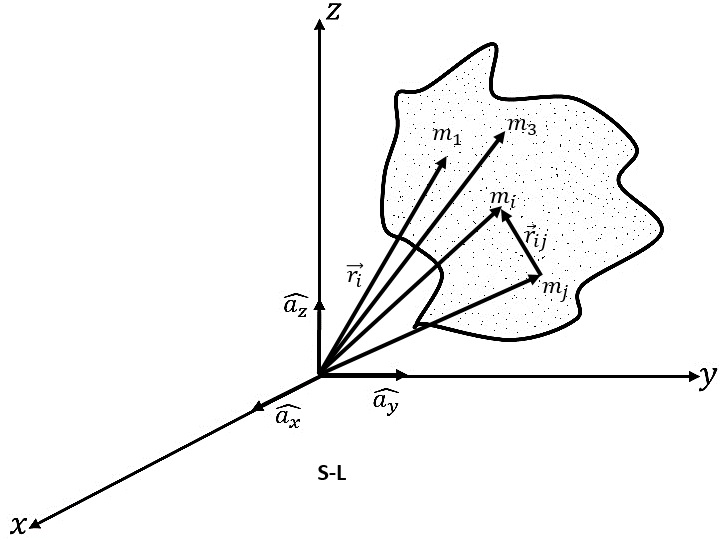
\includegraphics[width=5.94792in,height=4.43017in]{Imagenes/media/image43.jpeg}

Para este sistema se escribe la energía cinética para este sistema de la
forma:

\[T = \frac{1}{2}\sum_{\alpha = 1}^{n}m_{a}\sum_{i = 1}^{3}{\dot{x}}_{ai}^{\ \ \ \ 2}\ \ \ \ \ \ \ \ \ \ \]

La expresión (179) tiene una limitación y es que las coordenadas
cartesianas \({\dot{x}}_{ai}^{\ \ \ \ }\) no son coordenadas
independientes, por esta razón para la energía cinética \(T\) del
sistema de \(n -\)partículas en función de las coordenadas y velocidades
generalizadas, esto es:

\[x_{\alpha i} = x_{\alpha i}\left( q_{1},\ q_{2},q_{3},\ldots,q_{s};t \right)\]

\[{\dot{x}}_{\alpha i} = \sum_{j = 1}^{s}\frac{\partial x_{\alpha i}}{\partial q_{j}}{\dot{q}}_{j} + \frac{\partial x_{\alpha i}}{\partial t}\]

\[{\dot{x}}_{\alpha i} = \frac{\partial x_{\alpha i}}{\partial q_{1}}\dot{q_{1}} + \frac{\partial x_{\alpha i}}{\partial q_{2}}\dot{q_{2}} + \frac{\partial x_{\alpha i}}{\partial q_{3}}\dot{q_{3}} + \ldots + \frac{\partial x_{\alpha i}}{\partial t}\]

De esta manera, la velocidad generalizada está dada por:

\[{\dot{x}}_{\alpha i}^{\ \ \ \ 2} = \left( \sum_{j = 1}^{s}\frac{\partial x_{\alpha i}}{\partial q_{j}}{\dot{q}}_{j} + \frac{\partial x_{\alpha i}}{\partial t} \right)^{2}\]

\[{\dot{x}}_{\alpha i}^{\ \ \ \ 2} = \sum_{j,k}^{}\frac{\partial x_{\alpha i}}{\partial q_{j}}\frac{\partial x_{\alpha i}}{\partial q_{k}}\dot{q_{j}}\dot{q_{k}} + 2\sum_{j,}^{}\frac{\partial x_{\alpha i}}{\partial q_{j}}\frac{\partial x_{\alpha i}}{\partial t}\dot{q_{j}} + \left( \frac{\partial x_{qi}}{\partial t} \right)^{2}\]

De este modo:

\[T = \sum_{\alpha = 1}^{n}{\sum_{i,j,k}^{}{\frac{1}{2}m_{\alpha}}}\frac{\partial x_{\alpha i}}{\partial q_{i}}\frac{\partial x_{\alpha i}}{\partial q_{k}}\dot{q_{j}}\dot{q_{k}} + \sum_{\alpha = 1}^{n}{m_{\alpha}\sum_{i,j}^{}{\frac{\partial x_{\alpha i}}{\partial q_{i}}\frac{\partial x_{\alpha i}}{\partial t}\dot{q_{j}} +}}\sum_{\alpha = 1}^{n}{\frac{1}{2}m_{\alpha}}\sum_{i}^{}\left( \frac{\partial x_{qi}}{\partial t} \right)^{2}\]

Haciendo:

\[a_{jk} = \sum_{\alpha = 1}^{n}{\sum_{i,}^{}{\frac{1}{2}m_{\alpha}}}\frac{\partial x_{\alpha i}}{\partial q_{i}}\frac{\partial x_{\alpha i}}{\partial q_{k}}\]

\[b_{j} = \sum_{\alpha = 1}^{n}{\sum_{i,}^{}{m_{\alpha}\frac{\partial x_{\alpha i}}{\partial q_{i}}\frac{\partial x_{\alpha i}}{\partial t}}}\]

\[c = {\sum_{\alpha = 1}^{n}{\sum_{i}^{}{{\frac{1}{2}m}_{\alpha}\left( \frac{\partial x_{\alpha i}}{\partial t} \right)}}}^{2}\]

Entonces:

\[\mathbf{T =}\sum_{\mathbf{j,k}}^{}{\mathbf{a}_{\mathbf{j,k}}{\dot{\mathbf{q}}}_{\mathbf{j}}}{\dot{\mathbf{q}}}_{\mathbf{k}}\mathbf{+}\sum_{\mathbf{j}}^{}\mathbf{b}_{\mathbf{i}}{\dot{\mathbf{q}}}_{\mathbf{j}}\mathbf{+ c\ \ \ \ \ \ \ }\]

\uline{Simetría I: Homogeneidad del Tiempo}

La homogeneidad del tiempo~intenta explicar que el transcurrir de los
acontecimientos no modifica las leyes de la Física, esto es, que las
leyes de la física en un instante dado son las mismas que en cualquier
instante anterior y seguirán siendo las mismas en los instantes
posteriores.

El sistema de \(n -\)partículas es un sistema cerrado, por lo tanto,
cualquier tipo de observable es independiente del tiempo, por lo tanto
los coeficientes \(b_{j}\) y \(c\) son cero, de esta forma:

\[T = \sum_{j,k}^{}{a_{j,k}{\dot{q}}_{j}}{\dot{q}}_{k}\ \ \ \ \ \ \ \]

A partir de (181) se da que:

\[\frac{\partial T}{\partial{\dot{q}}_{l}} = \sum_{j}^{}{a_{j}{\dot{q}}_{j}} + \sum_{k}^{}a_{k}{\dot{q}}_{k}\]

\[\sum_{l}^{}\frac{\partial T}{\partial{\dot{q}}_{l}}{\dot{q}}_{l} = \sum_{j,l}^{}{a_{j,l}{\dot{q}}_{j}}{\dot{q}}_{l} + \sum_{j,l}^{}{a_{k,l}{\dot{q}}_{k}}{\dot{q}}_{l}\]

Como los subíndices son mudos:

\[\sum_{j}^{}\frac{\partial T}{\partial{\dot{q}}_{j}}{\dot{q}}_{j} = 2\sum_{j,k}^{}{a_{j,k}{\dot{q}}_{j}}{\dot{q}}_{k} = 2T\]

\[\sum_{j}^{}{\frac{\partial T}{\partial{\dot{q}}_{j}}{\dot{q}}_{j} = 2T}\]

Escribiendo el Lagrangiano:

\[L = L\left( q_{j},{\dot{q}}_{j};t \right)\]

\[\frac{dL}{dt} = \sum_{j}^{}{\frac{\partial L}{\partial q_{j}}{\dot{q}}_{j}} + \sum_{j}^{}{\frac{\partial L}{\partial{\dot{q}}_{j}}{\ddot{q}}_{j}} + \frac{\partial L}{\partial t}\]

Para sistemas cerrados o sistemas termodinámicos, el último término se
hace cero, así:

\[\frac{dL}{dt} = \sum_{j}^{}{\frac{d}{dt}\left( \frac{\partial L}{\partial{\dot{q}}_{j}} \right){\dot{q}}_{j}} + \sum_{j}^{}{\frac{\partial L}{\partial{\dot{q}}_{j}}{\ddot{q}}_{j}}\]

\[\sum_{j}^{}{\frac{d}{dt}\left\lbrack \left( \frac{\partial L}{\partial{\dot{q}}_{j}} \right){\dot{q}}_{j} \right\rbrack} = \sum_{j}^{}{\frac{d}{dt}\left( \frac{\partial L}{\partial{\dot{q}}_{j}} \right){\dot{q}}_{j}} + \sum_{j}^{}{\frac{\partial L}{\partial{\dot{q}}_{j}}{\ddot{q}}_{j}}\]

\[\frac{dL}{dt} = \sum_{j}^{}{\frac{d}{dt}\left\lbrack \left( \frac{\partial L}{\partial{\dot{q}}_{j}} \right){\dot{q}}_{j} \right\rbrack}\]

De esta manera:

\[\frac{d}{dt}\left( \sum_{j}^{}{\frac{\partial L}{\partial{\dot{q}}_{j}}{\dot{q}}_{j} - L} \right) = 0\ \ \ \ \ \ \]

La expresión (182) es consecuencia de un teorema de conservación, para
que esta igualdad se cumpla, debe darse que lo que se encuentra dentro
de los paréntesis sea una constante, por conveniencia se va a denotar
por \(H\), así:

\[\sum_{j}^{}{\frac{\partial L}{\partial{\dot{q}}_{j}}{\dot{q}}_{j} - L} = H\]

\[\sum_{j}^{}{\frac{\partial}{\partial{\dot{q}}_{j}}(T - U){\dot{q}}_{j} - L} = H\]

\[\sum_{j}^{}{\frac{\partial T}{\partial{\dot{q}}_{j}}{\dot{q}}_{j} - \sum_{j}^{}{\frac{\partial U}{\partial{\dot{q}}_{j}}{\dot{q}}_{j} -}L} = H\]

\[\sum_{j}^{}{\frac{\partial T}{\partial{\dot{q}}_{j}}{\dot{q}}_{j} - L} = H\ \ \ \ \ \ \ \ \]

Trayendo (182) a (184) y recordando que \(L = T - U\) entonces:

\[2T - (T - U) = H\]

\[T + U = H\ \ \ \ \ \ \ \ \]

La expresión (185) corresponde al teorema de conservación de la energía
total en los sistemas mecánicos holónomos esclerónomos, aquellos
sistemas sometidos a condiciones de ligadura independientes del tiempo
expresables mediante relaciones matemáticas entre sus coordenadas, no
sometidos a fuerzas de disipación, resulta ser una consecuencia
inmediata de la homogeneidad del tiempo, es decir, del hecho de que las
magnitudes fundamentales no dependen explícitamente del transcurrir del
tiempo.

\emph{\textbf{Homogeneidad del tiempo y del Espacio.}}

\[L = L(q_{1},\ q_{2},\ q_{3},\ldots,\ q_{j},\ \dot{q_{1}},\ \dot{q_{2}},\ \dot{q_{3}},\ldots,\dot{q_{J}};t)\]

\[\delta L = \sum_{}^{}{\frac{\partial L}{\partial q_{j}}\delta q_{j}} + \sum_{}^{}{\frac{\partial L}{\partial{\dot{q}}_{j}}\delta{\dot{q}}_{j} = 0}\]

\[\delta L = \sum_{}^{}{\frac{\partial L}{\partial q_{j}}\delta q_{j}} + \sum_{}^{}{\frac{\partial L}{\partial{\dot{q}}_{j}}\delta\frac{{\partial q}_{j}}{\partial t} = 0}\]

\[\frac{d}{dt}\left( \frac{\partial L}{\partial{\dot{q}}_{j}} \right) - \frac{\partial L}{\partial q_{j}} = 0\]

\[\delta L = \sum_{}^{}{\frac{d}{dt}\left( \frac{\partial L}{\partial{\dot{q}}_{j}} \right)\delta q_{j}}\ \  = 0\]

\[\frac{d}{dt}\left( \frac{\partial L}{\partial{\dot{q}}_{j}} \right) = 0\]

\[\frac{\partial L}{\partial{\dot{q}}_{j}} = p_{j} = cte\]

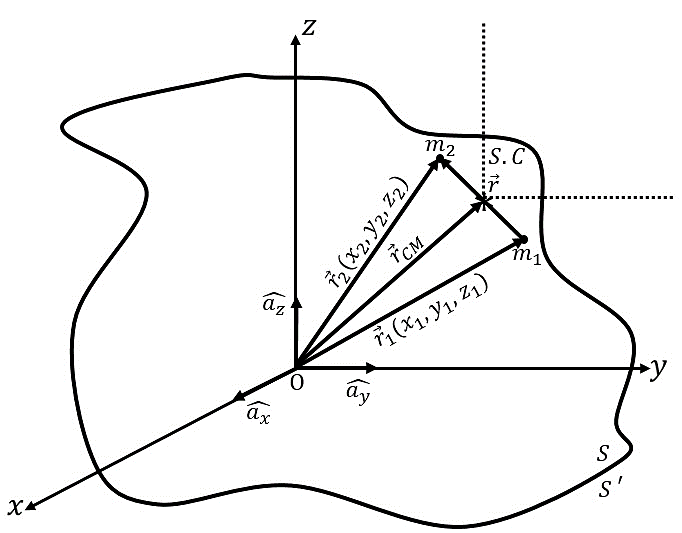
\includegraphics[width=5.98456in,height=4.67708in]{Imagenes/media/image44.png}\textbf{LAGRANGIANO
DE UN SISTEMA DE DOS PARTÍCULAS}

Tómese el sistema mostrado en la \emph{figura 27:}

\({\overrightarrow{r}}_{1}\) y \({\overrightarrow{r}}_{2}\) son vectores
posición de las partículas \(m_{1}\) y \(m_{2}\) con respecto al sistema
de referencia \(O\) inercial, estos vectores son por consiguiente:

\[{\overrightarrow{r}}_{1} = x_{1}\widehat{a_{x}} + y_{1}\widehat{a_{y}} + z_{1}\widehat{a_{z}}\]

\[{\overrightarrow{r}}_{2} = x_{2}\widehat{a_{x}} + y_{2}\widehat{a_{y}} + z_{2}\widehat{a_{z}}\]

Es de notar que el vector \(\overrightarrow{r}\) no está medido en el
sistema \(O\).

Como se trata de un sistema de dos partículas; su centro de masa se
considera, así:

\[{\overrightarrow{r}}_{cm} = x_{cm}\widehat{a_{x}} + y_{cm}\widehat{a_{y}} + z_{cm}\widehat{a_{z}}\]

Por simple suma vectorial, se tiene también que:

\[{\overrightarrow{r}}_{1} + \overrightarrow{r} = {\overrightarrow{r}}_{2}\]

\[\overrightarrow{r} = {\overrightarrow{r}}_{2} - {\overrightarrow{r}}_{1}\]

De esta manera:

\[\overrightarrow{r} = \left( x_{2} - x_{1} \right)\widehat{a_{x}} + (y_{2} - y_{1})\widehat{a_{y}} + (z_{2} - z_{1})\widehat{a_{z}}\]

Luego; el Lagrangiano del sistema es:

\[L = \frac{1}{2}\left( m_{1} + m_{2} \right){{\overrightarrow{\dot{r}}}_{cm}}^{2} + \frac{1}{2}m_{1}{{\overrightarrow{\dot{r}}}_{1}}^{2} + \frac{1}{2}m_{2}{{\overrightarrow{\dot{r}}}_{2}}^{2} - U\left( {\overrightarrow{r}}_{cm},\ {\overrightarrow{r}}_{1},{\overrightarrow{r}}_{2},{\overrightarrow{\dot{r}}}_{cm},{\overrightarrow{\dot{r}}}_{1},{\overrightarrow{\dot{r}}}_{2};t \right)\ \ \ \]

El Lagrangiano escrito en la ecuación (87) es muy complicado de
analizar, por ahora se va a analizar la dinámica en un nuevo sistema de
observación, llamado sistema centro de masa.

\[{\overrightarrow{r}}_{cm} = \frac{m_{1}{\overrightarrow{r}}_{1} + m_{2}{\overrightarrow{r}}_{2}}{m_{1} + m_{2}}\]

\[\left( m_{1} + m_{2} \right){\overrightarrow{r}}_{cm} = m_{1}{\overrightarrow{r}}_{1} + m_{2}{\overrightarrow{r}}_{2}\]

\[\left( m_{1} + m_{2} \right){\overrightarrow{r}}_{cm} = m_{1}{\overrightarrow{r}}_{1} + m_{2}\left( {\overrightarrow{r}}_{1} + \overrightarrow{r} \right)\]

\[\left( m_{1} + m_{2} \right){\overrightarrow{r}}_{cm} = \left( m_{1} + m_{2} \right){\overrightarrow{r}}_{1} + m_{2}\overrightarrow{r}\]

\[{\overrightarrow{r}}_{1} = {\overrightarrow{r}}_{cm} - \frac{m_{2}}{m_{1} + m_{2}}\overrightarrow{r}\ \ \]

Análogamente:

\[{\overrightarrow{r}}_{2} = {\overrightarrow{r}}_{cm} + \frac{m_{1}}{m_{1} + m_{2}}\overrightarrow{r}\]

\(x_{cm} = 0\), \(y_{cm} = 0\) y \(z_{cm} = 0\); entonces
\({\overrightarrow{r}}_{cm} = 0\). En el sistema \(C\) de referencia
\({\overrightarrow{\dot{r}}}_{cm} = 0\), por lo que se puede ver que en
la ecuación (87) se cancela el primer término.

\[{\overrightarrow{\dot{r}}}_{1} = {\overrightarrow{\dot{r}}}_{cm} - \frac{m_{2}}{m_{1} + m_{2}}\overrightarrow{\dot{r}}\]

\[{\overrightarrow{\dot{r}}}_{2} = {\overrightarrow{\dot{r}}}_{cm} + \frac{m_{1}}{m_{1} + m_{2}}\overrightarrow{\dot{r}}\]

Ahora, se procede a obtener el Lagrangiano para el \(S - C\):

\[L = \frac{1}{2}m_{1}{{\overrightarrow{\dot{r}}}_{1}}^{2} + \frac{1}{2}m_{2}{{\overrightarrow{\dot{r}}}_{2}}^{2} - U\left( \overrightarrow{r} \right)\]

Como bien se sabe \(U(\overrightarrow{r})\) proviene de una fuerza, ya
que
\(\overrightarrow{F} = - \overrightarrow{\nabla}U\left( \overrightarrow{r} \right)\),
retomando:

\[L = \frac{1}{2}m_{1}\left( \frac{m_{2}}{m_{1} + m_{2}} \right)^{2}{\overrightarrow{\dot{r}}}^{2} + \frac{1}{2}m_{2}\left( \frac{m_{1}}{m_{1} + m_{2}} \right)^{2}{\overrightarrow{\dot{r}}}^{2} - U\left( \overrightarrow{r} \right)\]

\[L = \frac{1}{2}\frac{m_{1}m_{2}}{m_{1} + m_{2}}\left( \frac{m_{2}}{m_{1} + m_{2}} \right){\overrightarrow{\dot{r}}}^{2} + \frac{1}{2}\frac{m_{1}m_{2}}{m_{1} + m_{2}}\left( \frac{m_{1}}{m_{1} + m_{2}} \right){\overrightarrow{\dot{r}}}^{2} - U\left( \overrightarrow{r} \right)\]

\[L = \frac{1}{2}\frac{m_{1}m_{2}}{m_{1} + m_{2}}{\overrightarrow{\dot{r}}}^{2}\left( \frac{m_{2}}{m_{1} + m_{2}} + \frac{m_{1}}{m_{1} + m_{2}} \right) - U\left( \overrightarrow{r} \right)\]

\[L = \frac{1}{2}\frac{m_{1}m_{2}}{m_{1} + m_{2}}{\overrightarrow{\dot{r}}}^{2} - U\left( \overrightarrow{r} \right)\]

Si se hace:

\[\mu = \frac{m_{1}m_{2}}{m_{1} + m_{2}}
\]

\[\mathbf{L =}\frac{\mathbf{1}}{\mathbf{2}}\mathbf{\mu}{\overrightarrow{\dot{\mathbf{r}}}}^{\mathbf{2}}\mathbf{- U}\left( \overrightarrow{\mathbf{r}} \right)\]

La expresión (12) corresponde al Lagrangiano de dos partículas reducido
al movimiento de una sola partícula pero como masa reducida.

\textbf{TEOREMAS DE CONSERVACIÓN, PRIMERA Y SEGUNDA LEY DE KEPLER}

En física, los teoremas de conservación hacen referencia a los
planteamientos que postulan que durante la evolución de un sistema
aislado, algunas de las magnitudes involucradas en el sistema poseen un
valor que permanece constante.

La conservación de alguna magnitud física en mecánica clásica conlleva a
la existencia de una simetría en el Lagrangiano, trabajo que fue
realizado por la matemática alemana Emmy Noether.

Un formalismo Lagrangiano admite en las teorías físicas una prueba de
que los teoremas de conservación están asociados a una propiedad de
simetría presentada por el espacio donde se encuentra el sistema.

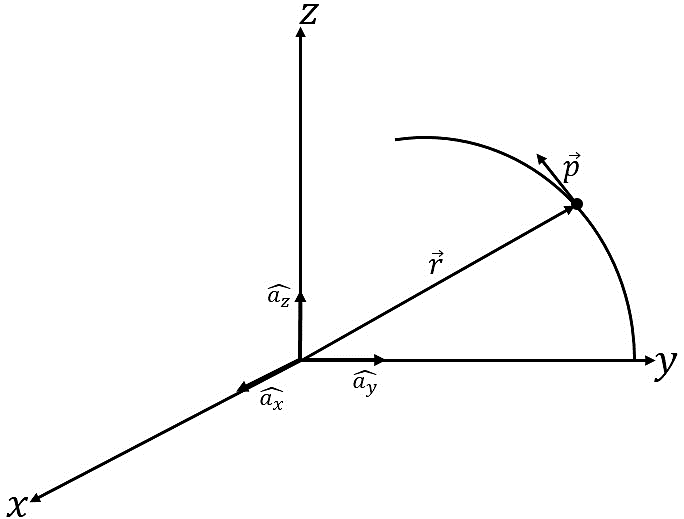
\includegraphics[width=5.78125in,height=4.38665in]{Imagenes/media/image45.png}Piénsese
en el movimiento rotacional donde el eje \(z\) sea un eje de giro tal
como se muestra en la \emph{figura 28}:

Se tiene que el momento angular está definido como:

\[\overrightarrow{L} = \overrightarrow{r} \times \overrightarrow{p}\]

Así mismo, la variación temporal del momento angular conlleva a obtener
el momento de rotación, así:

\[\frac{d\overrightarrow{L}}{dt} = \overrightarrow{\tau} = \frac{d\overrightarrow{r}}{dt} \times \overrightarrow{p} + \overrightarrow{r} \times \frac{d\overrightarrow{p}}{dt}\]

\[\overrightarrow{\tau} = \overrightarrow{v} \times \left( m\overrightarrow{v} \right) + \overrightarrow{r} \times \overrightarrow{F}\]

Nótese
\(\overrightarrow{v} \times \left( m\overrightarrow{v} \right) = 0\) ya
que \(\overrightarrow{v}\) es paralelo a
\(\left( m\overrightarrow{v} \right)\), de esta manera:

\[\overrightarrow{\tau} = \overrightarrow{r} \times \overrightarrow{F}\]

\[\overrightarrow{\tau} = \left( x\widehat{a_{x}} + y\widehat{a_{y}} + z\widehat{a_{z}} \right) \times \left( F_{x}\widehat{a_{x}} + F_{y}\widehat{a_{y}} + F_{z}\widehat{a_{z}} \right)\]

Es decir:

\[\overrightarrow{\tau} = \left| \begin{matrix}
\widehat{a_{x}} & \widehat{a_{y}} & \widehat{a_{z}} \\
x & y & z \\
F_{x} & F_{y} & F_{z} \\
\end{matrix} \right| = \left( yF_{z} - zF_{y} \right)\widehat{a_{x}} - \left( xF_{z} - zF_{x} \right)\widehat{a_{y}} + \left( xF_{y} - yF_{x} \right)\widehat{a_{z}}\]

Como:

\[\overrightarrow{\tau} = \tau_{x}\widehat{a_{x}} + \tau_{y}\widehat{a_{y}} + \tau_{z}\widehat{a_{z}}\]

Se puede ver que:

\[\tau_{x} = yF_{z} - zF_{y}\]

\[\tau_{y} = - xF_{z} + zF_{x}\]

\[\tau_{z} = xF_{y} - yF_{x}\]

Donde \(\tau_{x} = 0\), \(\tau_{y} = 0\) y \(\tau_{z} \neq 0\), por lo
que es posible considerar que el movimiento se debe dar u ocurre en el
plano \(xy\), así:

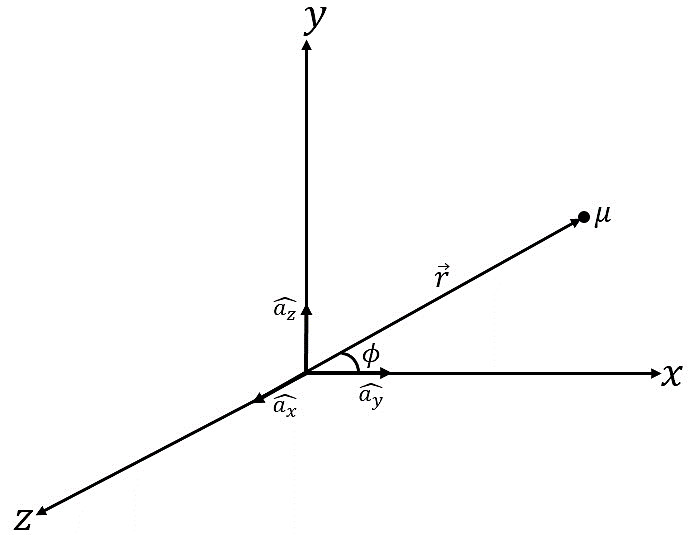
\includegraphics[width=6.0625in,height=4.69375in]{Imagenes/media/image46.png}

\[\overrightarrow{r} = x\widehat{a_{x}} + y\widehat{a_{y}}\]

\[\cos\phi = \frac{x}{r}\]

\[{sen}\phi = \frac{y}{r}\]

De esta manera:

\[\overrightarrow{r} = r\cos\phi\widehat{a_{x}} + r{sen}\phi\widehat{a_{y}}\]

Es de recordar que
\(\cos\phi\widehat{a_{x}} + {sen}\phi\widehat{a_{y}} = \widehat{a_{r}}\),
por lo que:

\[\overrightarrow{r} = r\widehat{a_{r}}\]

Como ya se mostró para las coordenadas polares:

\[{\overrightarrow{\dot{r}}}^{2} = {\dot{r}}^{2} + r^{2}{\dot{\phi}}^{2}\]

Por lo tanto el Lagrangiano es:

\[\mathbf{L =}\frac{\mathbf{1}}{\mathbf{2}}\mathbf{\mu}\left( {\dot{\mathbf{r}}}^{\mathbf{2}}\mathbf{+}\mathbf{r}^{\mathbf{2}}{\dot{\mathbf{\phi}}}^{\mathbf{2}} \right)\mathbf{- U}\left( \mathbf{r} \right)\mathbf{\ \ \ \ \ }\]

El Lagrangiano escrito en (90) genera un problema como dos grados de
libertad en el sistema \(S - C\).

La coordenada generalizada \(\phi\) no aparece explícitamente en el
Lagrangiano y se llama \emph{coordenada cíclica o ignorable} esto indica
que el momento angular se conserva, siendo este uno de los teoremas de
conservación.

Escribiendo la ecuación de movimiento para \(\phi\), se tiene:

\[\frac{\partial L}{\partial\dot{\phi}} = \mu r^{2}\dot{\phi},\ \ \ \ \ \ \ \ \frac{\partial L}{\partial\phi} = 0\]

\[\frac{d}{dt}\left( \mu r^{2}\dot{\phi} \right) = 0\ \ \ \ \]

En la expresión (92) se hace necesario introducir el concepto de
integral primera de movimiento. Se denomina integral de movimiento a una
función que depende de la posición y la velocidad que es constante
durante toda la trayectoria. El concepto se extiende en la teoría de
ecuaciones diferenciales ordinarias a integral primera de movimiento. La
integral primera de movimiento resulta constante cuando a las variables
de la ecuación diferencial y sus derivadas resulta constante cuando se
introduce en ella la dependencia respecto al tiempo o considerada
variable dependiente. De esta forma \(\mu r^{2}\dot{\phi}\) hace parte
de una integral primera de movimiento porque para que la ecuación (92)
se cumpla, esto debe ser constante.

Luego:

\[\mu r^{2}\dot{\phi} = cte = l\]

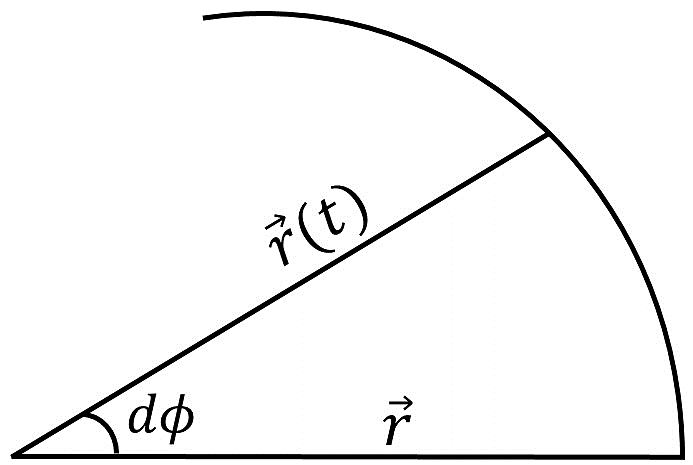
\includegraphics[width=3.97917in,height=3.19792in]{Imagenes/media/image47.png}A
partir de la \emph{figura 30} se cumple que:

\[dA = \frac{1}{2}r(rd\phi)\]

\[\frac{dA}{dt} = \frac{1}{2}r^{2}\frac{d\phi}{dt} = \frac{1}{2}r^{2}\dot{\phi}\]

Como:

\[\dot{\phi} = \frac{l}{\mu r^{2}}\]

Entonces:

\[\frac{dA}{dt} = \frac{1}{2}r^{2}\frac{l}{\mu r^{2}} = \frac{l}{2\mu} = cte\]

Luego:

\[\frac{\mathbf{dA}}{\mathbf{dt}}\mathbf{= cte\ \ \ \ }\]

La expresión (93) indica que un radio vector barre áreas iguales en
tiempos iguales y es lo concerniente a la SEGUNDA LEY DE KEPLER. Esto va
asociado a una propiedad de simetría del espacio y el tiempo. Detrás de
todo teorema de conservación hay una propiedad de simetría.

Hay otra integral primera de movimiento asociada con el teorema de
conservación de la energía, expresada como:

\[E = T + U\]

\[E = \frac{1}{2}\mu{\dot{r}}^{2} + \frac{1}{2}\mu r^{2}{\dot{\phi}}^{2} + U(r)\]

\[E - U(r) - \frac{1}{2}\mu r^{2}{\dot{\phi}}^{2} = \frac{1}{2}\mu{\dot{r}}^{2}\]

\[\frac{dr}{dt} = \sqrt{\frac{2}{\mu}\left\lbrack E - U(r) - \frac{1}{2}\mu r^{2}\frac{l^{2}}{\mu^{2}r^{4}} \right\rbrack}\]

\[dt = \frac{dr}{\sqrt{\frac{2}{\mu}\left\lbrack E - U(r) - \frac{l^{2}}{2\mu r^{2}} \right\rbrack}}\]

Como:

\[\dot{\phi} = \frac{l}{\mu r^{2}}\]

\[\frac{d\phi}{dt} = \frac{l}{\mu r^{2}}\]

\[d\phi = dt\frac{l}{\mu r^{2}}\]

\[dt = \frac{\mu r^{2}}{l}d\phi\]

Entonces:

\[\frac{\mu r^{2}}{l}d\phi = \frac{dr}{\sqrt{\frac{2}{\mu}\left\lbrack E - U(r) - \frac{l^{2}}{2\mu r^{2}} \right\rbrack}}\]

\[\int_{\phi_{o}}^{\phi}{d\phi} = \int_{r_{\min}}^{r}\frac{\frac{l}{r^{2}}dr}{\sqrt{\frac{2\mu^{2}}{\mu}\left\lbrack E - U(r) - \frac{l^{2}}{2\mu r^{2}} \right\rbrack}}\]

\[\phi - \phi_{o} = \int_{r_{\min}}^{r}\frac{\frac{l}{r^{2}}dr}{\sqrt{2\mu\left\lbrack E - U(r) - \frac{l^{2}}{2\mu r^{2}} \right\rbrack}}\]

\[\mathbf{\phi -}\mathbf{\phi}_{\mathbf{o}}\mathbf{=}\int_{\mathbf{r}_{\mathbf{\min}}}^{\mathbf{r}}\frac{\frac{\mathbf{l}}{\mathbf{r}^{\mathbf{2}}}\mathbf{dr}}{\sqrt{\mathbf{2}\mathbf{\mu}\left\lbrack \mathbf{E - U}\left( \mathbf{r} \right) \right\rbrack\mathbf{-}\frac{\mathbf{l}^{\mathbf{2}}}{\mathbf{r}^{\mathbf{2}}}}}\]

La ecuación (94) corresponde a la formulación matemática de la PRIMERA
LEY DE KEPLER o también llamada LEY DE ÓRBITAS.

\textbf{ECUACIÓN DIFERENCIAL PARA DETERMNAR EL TIPO DE ÓRBITA}

La ecuación diferencial para determinar el tipo de órbita es conveniente
tratarla en coordenadas polares, el tratamiento a realizar conllevará a
esto de manera natural donde el movimiento de un cuerpo que se encuentra
bajo la influencia de una fuerza de tipo central estará en el centro de
dicha fuerza con el fin de llevarla al origen.

Analícese la ecuación de movimiento para la coordenada generalizada
\(r\) a partir del Lagrangiano escrito en la ecuación (91), así:

\[\mathbf{L =}\frac{\mathbf{1}}{\mathbf{2}}\mathbf{\mu}\left( {\dot{\mathbf{r}}}^{\mathbf{2}}\mathbf{+}\mathbf{r}^{\mathbf{2}}{\dot{\mathbf{\phi}}}^{\mathbf{2}} \right)\mathbf{- U}\left( \mathbf{r} \right)\mathbf{\ \ }\]

\[\frac{\partial L}{\partial\dot{r}} = \mu\dot{r},\ \ \ \ \ \ \frac{\partial L}{\partial r} = \mu r{\dot{\phi}}^{2} - \frac{\partial U}{\partial r}\]

Luego:

\[\frac{d}{dt}\left( \mu\dot{r} \right) - \mu r{\dot{\phi}}^{2} + \frac{\partial U}{\partial r} = 0\]

\[\mu\ddot{r} - \mu r{\dot{\phi}}^{2} = - \frac{\partial U}{\partial r}\]

\[\mu\ddot{r} = - \frac{\partial U}{\partial r} + \mu r{\dot{\phi}}^{2}\ \ \ \ \]

\[\mu\ddot{r} = - \frac{\partial U}{\partial r} + \mu r\frac{l^{2}}{\mu^{2}r^{4}}\]

\[\mu\ddot{r} = - \frac{\partial U}{\partial r} + \frac{l^{2}}{{\mu r}^{3}}\]

El segundo término de la expresión (95) corresponde a una fuerza
centrífuga. Ahora, es necesario introducir el concepto de \emph{fuerza
efectiva} que posteriormente conllevará a un \emph{potencial efectivo}.
La fuerza efectiva se puede definir como la fuerza en dirección radial
más la fuerza centrífuga, en otros términos se puede ver como el
producto entre la masa efectiva y la aceleración, de esta manera:

\[\mu\ddot{r} = {\overrightarrow{F}}_{r} + {\overrightarrow{F}}_{CEN}\]

Sea \(\mu\ddot{r} = F_{EFEC}^{'}\), así:

\[F_{EFEC}^{'} = {\overrightarrow{F}}_{r} + {\overrightarrow{F}}_{CEN}\]

Como ya se sabe, la energía total es:

\[E = \frac{1}{2}\mu{\dot{r}}^{2} + \frac{1}{2}\mu r^{2}{\dot{\phi}}^{2} + U(r)\]

Ya corresponde a la suma de la energía y el potencial, en este caso ya
no es un potencial real, sino un potencial efectivo, es decir:

\[E = T + U_{EFEC}^{'}(r)\]

Igualando las expresiones (97) y (98), se tiene:

\[\frac{1}{2}\mu{\dot{r}}^{2} + \frac{1}{2}\mu r^{2}{\dot{\phi}}^{2} + U(r) = T + U_{EFEC}^{'}(r)\]

Como:

\[\dot{\phi} = \frac{l}{\mu r^{2}}\]

Entonces:

\[U_{EFEC}^{'}(r) = U(r) + \frac{1}{2}\mu r^{2}\frac{l^{2}}{\mu^{2}r^{4}}\]

Así:

\[F_{EFEC}^{'}(r) = - \frac{\partial U_{EFEC}^{'}(r)}{\partial r} = - \frac{\partial U}{\partial r} - \frac{\partial}{\partial r}(\frac{l^{2}}{\mu^{}r^{2}})\]

\[F_{EFEC}^{'}(r) = - \frac{\partial U}{\partial r} + \frac{l^{2}}{\mu r^{3}}\]

Luego:

\[\mu\ddot{r} - \mu r{\dot{\phi}}^{2} = - \frac{\partial U}{\partial r}\]

\[\mu\ddot{r} - \frac{l^{2}}{\mu r^{3}}\  = - \frac{\partial U}{\partial r}\ \]

Sea:

\[u = \frac{1}{r}\]

Se cumple que:

\[\frac{du}{d\phi} = - \frac{1}{r^{2}}\frac{dr}{d\phi}\frac{dt}{dt} = - \frac{1}{r^{2}}\frac{\dot{r}}{\dot{\varnothing}} = - \frac{\mu\dot{r}}{l}\]

\[\frac{d^{2}u}{d\phi^{2}} = \frac{d}{d\phi}\left( \frac{du}{d\phi} \right) = \frac{d}{d\phi}\left( - \frac{\mu\dot{r}}{l} \right)\frac{dt}{dt} = - \frac{\mu}{l\dot{\phi}}\frac{d}{dt}\left( \dot{r} \right)\]

\[\frac{d^{2}u}{d\phi^{2}} = - \frac{\mu}{l\frac{l}{\mu r^{2}}}\ddot{r} = - \frac{\mu^{2}r^{2}}{l^{2}}\ddot{r}\]

De esta manera:

\[\ddot{r} = - \frac{l^{2}}{\mu^{2}r^{2}}\frac{d^{2}u}{d\phi^{2}} = - \frac{l^{2}}{\mu^{2}}u^{2}\frac{d^{2}u}{d\phi^{2}}\]

Reemplazando en (99) ­­se tiene que:

\[\mu\left( - \frac{l^{2}}{\mu^{2}}u^{2}\frac{d^{2}u}{d\phi^{2}} - \frac{l^{2}}{\mu^{2}}u^{3} \right) = F\left( \frac{1}{u} \right)\]

\[- \frac{l^{2}}{\mu}u^{2}\left( \frac{d^{2}u}{d\phi^{2}} + u \right) = F(u)\]

Finalmente:

\[\frac{d^{2}u}{d\phi^{2}} + u = - \frac{\mu}{l^{2}}\left( \frac{1}{u^{2}} \right)F(u)\]

La expresión (100) corresponde a la ecuación diferencial para conocer el
tipo de órbita, es necesario tener el tipo de fuerzas para poder hallar
de una manera precisa el tipo de órbita.

\textbf{PARTÍCULA BAJO LA ACCIÓN DE UNA FUERZA DE UN FUERZA DE TIPO
CENTRAL DE LA FORMA}
\(\widehat{\mathbf{F}}\mathbf{= -}\frac{\mathbf{K}}{\mathbf{r}^{\mathbf{2}}}\widehat{\mathbf{a}_{\mathbf{r}}}\)

Inicialmente se tiene que de acuerdo al tipo de fuerza existe un
potencial real que está dado por:

\[\int_{U_{\infty}}^{U}{dU} = \int_{\infty}^{r}{kr^{- 2}}dr\]

\[U - U_{\infty} = - \left. \ \frac{k}{r} \right\rfloor_{\infty}^{r}\]

Es de tener en cuenta que el potencial en el infinito es igual a cero,
por lo tanto:

\[U(r) = - \frac{k}{r}\]

Ahora, utilizando la ecuación diferencial para el tipo de órbita escrita
en (100) se tiene:

Recordar cambio de variable \(
\)

\[u = \frac{1}{r}\]

\[\frac{d^{2}u}{d\phi^{2}} + u = - \frac{\mu}{l^{2}}\left( \frac{1}{u^{2}} \right)\left( - ku^{2} \right)\]

\[\frac{d^{2}u}{d\phi^{2}} + u = \frac{k\mu}{l^{2}}\]

\[\frac{d^{2}u}{d\phi^{2}} + u - \frac{k\mu}{l^{2}} = 0\]

Haciendo:

\[u - \frac{k\mu}{l^{2}} = y\]

Entonces:

\[\frac{d^{2}y}{d\phi^{2}} + y = 0\ \ \ \ \ \ \ \ \]

La ecuación diferencial escrita en (101) tiene como solución:

\[y = C_{1}\cos\left( \phi - \phi_{0} \right)\]

\[u = C_{1}\cos{\left( \phi - \phi_{0} \right) + \frac{k\mu}{l^{2}}}\]

Como:

\[u = \frac{1}{r}\]

Se cumple que:

\[\frac{1}{r} = \frac{k\mu}{l^{2}} + C_{1}\cos\left( \phi - \phi_{0} \right)\]

Reescribiendo:

\[\frac{1}{r} = \frac{k\mu}{l^{2}}\left\lbrack 1 + \frac{l^{2}}{k\mu}C_{1}\cos\left( \phi - \phi_{0} \right) \right\rbrack\]

Sean:

\[\frac{l^{2}}{k\mu} = \alpha\ \ \ \ \ y\ \ \ \ \ \frac{l^{2}}{k\mu}C_{1} = \epsilon\]

Luego:

\[\frac{\mathbf{\alpha}}{\mathbf{r}}\mathbf{= 1 + \epsilon}\mathbf{\cos}\left( \mathbf{\phi -}\mathbf{\phi}_{\mathbf{0}} \right)\]

Es de notar que la ecuación (103) corresponde a la ecuación general de
una cónica, de acuerdo a la excentricidad \(\epsilon\) es que se
determina el tipo de órbita, esto es:

\begin{itemize}
\item
  \begin{quote}
  Si \(\epsilon > 1\) la órbita es hiperbólica.
  \end{quote}
\item
  \begin{quote}
  Si \(\epsilon = 1\) la órbita es parabólica.
  \end{quote}
\item
  \begin{quote}
  Si \(0 < \epsilon < 1\) la órbita es elíptica.
  \end{quote}
\item
  \begin{quote}
  Si \(\epsilon = 0\) la órbita es circular.
  \end{quote}
\end{itemize}

Analizando el mismo problema pero ahora con la ley de órbitas asociada
al teorema de la conservación de la energía, se da que antes de resolver
la integral es conveniente analizar los tipos de órbita gráficamente,
así, es de tener primero en cuenta que:

\[U_{EFEC}^{'}(r) = U(r) + \frac{l^{2}}{2\mu r^{2}}\]

\[U_{EFEC}^{'}(r) = - \frac{k}{r} + \frac{l^{2}}{2\mu r^{2}}\]

\[\dot{r} = \sqrt{\frac{2}{\mu}\left\lbrack E - U_{EFEC}^{'}(r) \right\rbrack}\]

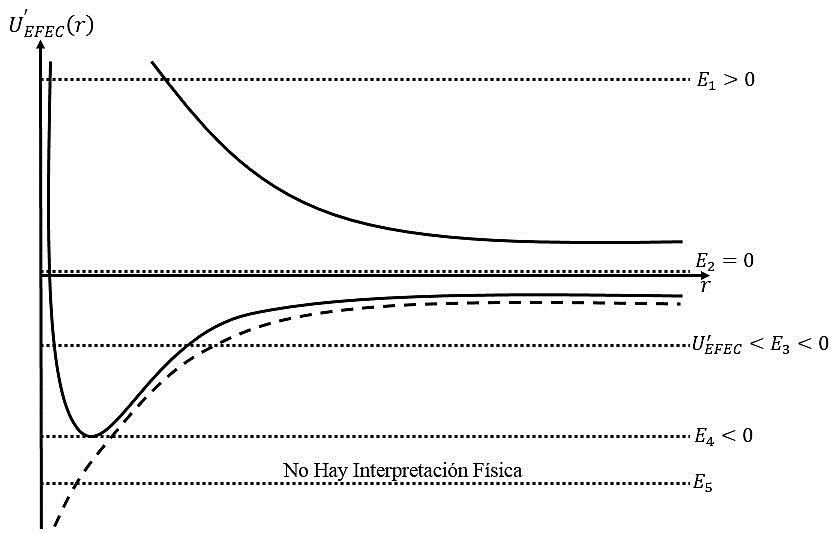
\includegraphics[width=6.94375in,height=4.41667in]{Imagenes/media/image48.png}Considérese
ahora la partícula en diferentes estados de energía:

Analícese cada región en cada uno de los estados energía.

\[\dot{r} = \sqrt{\frac{2}{\mu}\left\lbrack E - U_{EFEC}^{'}(r) \right\rbrack}\]

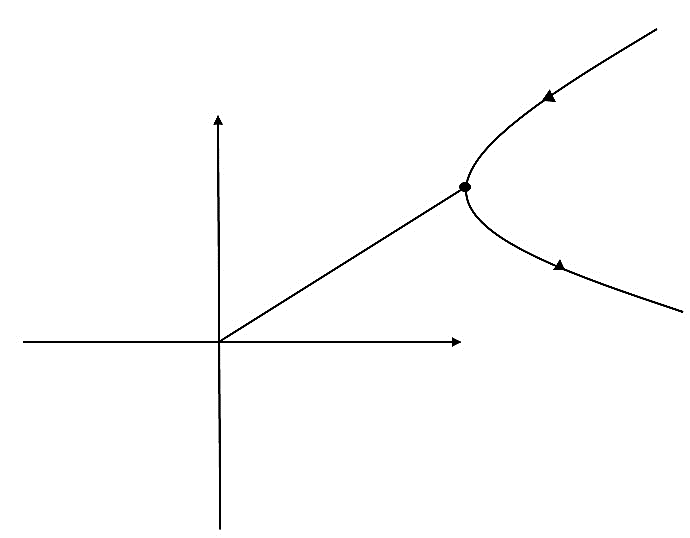
\includegraphics[width=3.91667in,height=3.05347in]{Imagenes/media/image49.png}REGIÓN
\(E_{1}\): En esta región \(r < r_{1}\), se tiene
\(U_{EFEC}^{'}(r) > E_{1}\) y \(\dot{r}\) es imaginario.

Órbita Abierta Hiperbólica.\\
Órbita Seguida por Cometas.

REGIÓN \(E_{2}\): Aquí \(U_{EFEC}^{'}(r) > E_{2}\) y \(\dot{r}\) es
imaginario.

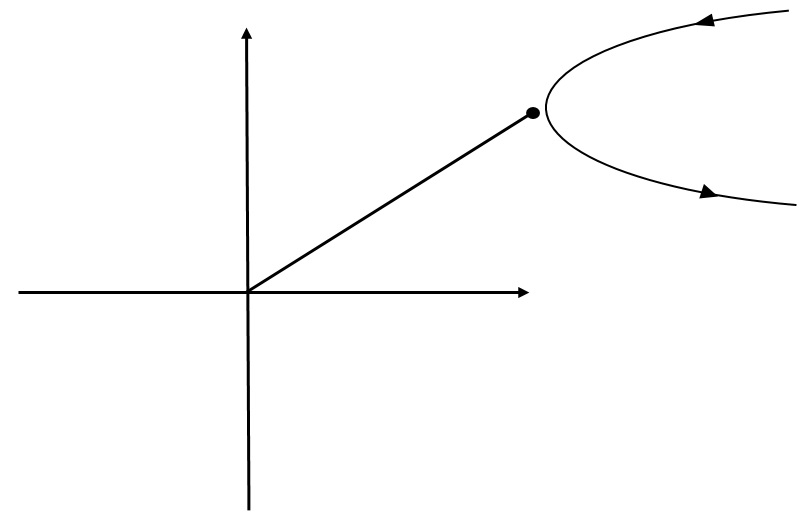
\includegraphics[width=4.2in,height=2.73264in]{Imagenes/media/image50.jpeg}

Órbita Abierta Parabólica.

REGIÓN \(E_{3}\): En esta región \(r_{3} \leq r \leq r_{4}\). Hay dos
puntos de retroceso denominados \emph{puntos absidales}. Se tiene una
trayectoria elíptica donde los ejes mayor y menor son dichos puntos de
retroceso. Se tiene que \(U_{EFEC}^{'}(r) < E_{3}\). \(\dot{r}\) es
real, \(r = r_{3}\) y \(r = r_{4}\). \(U_{EFEC}^{'}(r) = E_{3}\) esto
implica que bajo estas circunstancias la partícula está oscilando.

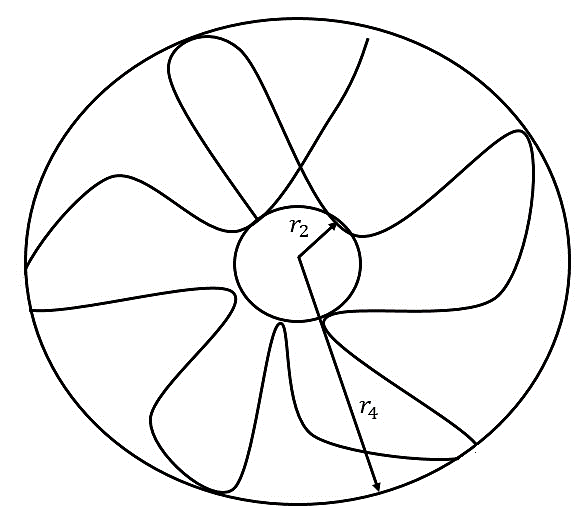
\includegraphics[width=4.19165in,height=3.6875in]{Imagenes/media/image51.png}

Órbita Cerrada Elíptica.\\
La Partícula Oscila.

REGIÓN \(E_{4}\): Aquí \(r = r_{0}\), \(U_{EFEC}^{'}(r) = 0\) y
\(\dot{r} = 0\). Es indica que \(r\) es constante y la órbita es
circular cerrada.

Retomando con la ley de órbitas se tiene:

\[\phi - \phi_{o} = \int_{r_{\min}}^{r}\frac{\frac{l}{r^{2}}dr}{\sqrt{2\mu\left\lbrack E - U(r) \right\rbrack - \frac{l^{2}}{r^{2}}}}\]

\[\phi - \phi_{o} = \int_{r_{\min}}^{r}\frac{\frac{l}{r^{2}}dr}{\sqrt{2\mu E + \frac{2\mu k}{r} - \frac{l^{2}}{r^{2}}}}\]

Por otro lado, cambiando la variable se tiene.

\[u = \frac{1}{r}\]

\[du = - \frac{1}{r^{2}}dr\]

\[dr = - \ r^{2}du\]

De esta manera:

\[\phi - \phi_{o} = - \int_{r_{\min}}^{r}\frac{\frac{l}{r^{2}}r^{2}du}{\sqrt{2\mu E + 2\mu ku - l^{2}u^{2}}}\]

\[\phi - \phi_{o} = - \int_{r_{\min}}^{r}\frac{du}{\sqrt{\frac{2\mu E}{l^{2}} + \frac{2\mu ku}{l^{2}} - u^{2}}}\]

Sean:

\[\frac{2\mu E}{l^{2}} = a,\ \ \ \ \ \ \frac{2\mu k}{l^{2}} = b\ \ \ \ y\ \ \  - 1 = c\]

Así:

\[\phi - \phi_{o} = - \int_{r_{\min}}^{r}{\frac{du}{\sqrt{\frac{2\mu E}{l^{2}} + \frac{2\mu ku}{l^{2}} - u^{2}}} = - \int_{r_{\min}}^{r}\frac{du}{\sqrt{a + bu + cu^{2}}}}\]

Esta integral tiene como solución:

\[- \int_{r_{\min}}^{r}\frac{du}{\sqrt{a + bu + cu^{2}}} = \frac{1}{\sqrt{- c}}arcocos\left( - \frac{b + 2cu}{\sqrt{b^{2} - 4ac}} \right)\]

Luego:

\[\phi - \phi_{o} = - \frac{1}{\sqrt{1}}arcocos\left\lbrack \frac{- \frac{2\mu k}{l^{2}} + 2u}{\sqrt{\left( \frac{2\mu k}{l^{2}} \right)^{2} + 4\frac{2\mu E}{l^{2}}}} \right\rbrack\]

\[\cos\left( \phi - \phi_{o} \right) = \frac{- \frac{2\mu k}{l^{2}}\left\lbrack 1 - \frac{l^{2}}{\mu k}u \right\rbrack}{\frac{2\mu k}{l^{2}}\sqrt{1 + \frac{2l^{2}E}{\mu k^{2}}}}\]

\[\cos\left( \phi - \phi_{o} \right) = \frac{\frac{l^{2}}{\mu k}u - 1}{\sqrt{1 + \frac{2l^{2}}{\mu k^{2}}E}}\]

\[\sqrt{1 + \frac{2l^{2}}{\mu k^{2}}E}\ cos\left( \phi - \phi_{o} \right) = \frac{l^{2}}{\mu k}u - 1\]

\[\frac{l^{2}}{\mu k}u = 1 + \sqrt{1 + \frac{2l^{2}}{\mu k^{2}}E}\ cos\left( \phi - \phi_{o} \right)\]

Sean:

\[\frac{l^{2}}{\mu k} = \alpha\ \ \ y\ \ \ \ \ \ \ \ \ \ \ \ \ \sqrt{1 + \frac{2l^{2}}{\mu k^{2}}E} = \epsilon\]

Además como:

\[u = \frac{1}{r}\]

Finalmente:

\[\frac{\mathbf{\alpha}}{\mathbf{r}}\mathbf{= 1 + \epsilon}\mathbf{\cos}\left( \mathbf{\phi -}\mathbf{\phi}_{\mathbf{0}} \right)\]

\[\sqrt{1 + \frac{2l^{2}}{\mu k^{2}}E} = \epsilon\]

Se obtuvo la misma ecuación general de una cónica tal como se obtuvo
utilizando la ecuación diferencial para el tipo de órbita, sólo que en
este caso la excentricidad es función de la energía, por lo tanto:

\begin{itemize}
\item
  \begin{quote}
  Si \(E > 0.\) En esta situación \(E_{1} > 0\), \(\epsilon > 0\) y la
  órbita es hiperbólica abierta.
  \end{quote}
\item
  \begin{quote}
  Si \(E = 0\). Para este caso \(E_{2} = 0\), \(\epsilon = 1\) y la
  órbita es parabólica abierta.
  \end{quote}
\item
  \begin{quote}
  Si \(U_{EFEC}^{'}{(r)}_{\min} < E_{3} < 0;\ 0 < \epsilon < 1\) y la
  órbita es elíptica.
  \end{quote}
\item
  \begin{quote}
  Si \(E = - \frac{\mu k^{2}}{2l^{2}}\), \(\epsilon = 0\) y la órbita es
  circular.
  \end{quote}
\end{itemize}

\textbf{TEOREMA DEL VIRIAL Y TERCERA LEY DE KEPLER}

El teorema del Virial corresponde a una expresión generalizada que
relaciona la energía cinética total promedio de un sistema con la
energía potencial del mismo. Esta definición está dada para la mecánica
clásica.

Cuando los sistemas poseen una gran cantidad de partículas, este teorema
permite calcular la energía cinética siendo este tipo de sistemas muy
complejos para manipular y tener una solución exacta.

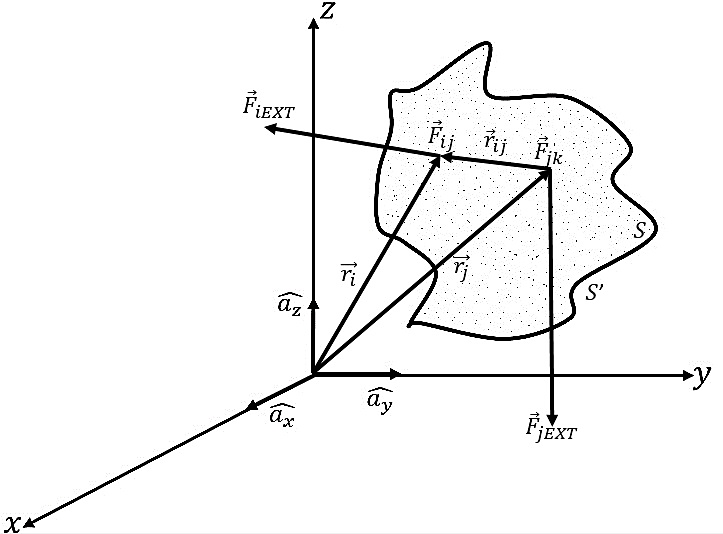
\includegraphics[width=5.95139in,height=4.38333in]{Imagenes/media/image52.png}Considérese
el sistema de \(n -\)partículas mostrado en la \emph{figura 35:}

Se sabe que:

\[\overrightarrow{{\dot{p}}_{i}} = {\overrightarrow{F_{i}}}_{T}\]

Como se trata de un sistema de \(n -\)partículas, entonces:

\[\sum_{i = 1}^{n}\overrightarrow{{\dot{p}}_{i}} = \sum_{i = 1}^{n}{\overrightarrow{F_{i}}}_{T}\]

De esta manera, se define el Virial como:

\[\mathbf{G =}\sum_{\mathbf{i = 1}}^{\mathbf{n}}{{\overrightarrow{\mathbf{p}}}_{\mathbf{i}}\mathbf{\cdot}}{\overrightarrow{\mathbf{r}}}_{\mathbf{i}}\mathbf{\ \ \ \ \ }\]

Obteniendo el cambio con respecto al tiempo de esta magnitud, se tiene:

\[\frac{dG}{dt} = \sum_{i = 1}^{n}{\frac{{d\overrightarrow{p}}_{i}}{dt} \cdot}{\overrightarrow{r}}_{i} + \sum_{i = 1}^{n}{\overrightarrow{p}}_{i} \cdot \frac{{d\overrightarrow{r}}_{i}}{dt}\]

\[\frac{dG}{dt} = \sum_{i = 1}^{n}{{\overrightarrow{F}}_{iT} \cdot}{\overrightarrow{r}}_{i} + \sum_{i = 1}^{n}m_{i}\mathbf{V}_{i} \cdot \mathbf{V}_{i}\ \ \ \ \ \]

Es de tener en cuenta que el segundo término de la ecuación (105) es dos
veces la energía cinética \(2E_{k}\), por lo tanto:

\[\frac{dG}{dt} = \sum_{i = 1}^{n}{\left( {\overrightarrow{F}}_{iEXT} + {\overrightarrow{F}}_{ij} \right) \cdot}{\overrightarrow{r}}_{i} + 2E_{k}\]

\[\frac{dG}{dt} = \sum_{i = 1}^{n}{{\overrightarrow{F}}_{iEXT} \cdot}{\overrightarrow{r}}_{i} + \sum_{i = 1}^{n}{{\overrightarrow{F}}_{ij} \cdot}{\overrightarrow{r}}_{i} + 2E_{k}\]

\[\frac{dG}{dt} = \sum_{i = 1}^{n}{{\overrightarrow{F}}_{iEXT} \cdot}{\overrightarrow{r}}_{i} + {\overrightarrow{F}}_{12} \cdot {\overrightarrow{r}}_{1} + {\overrightarrow{F}}_{13} \cdot {\overrightarrow{r}}_{1} + \ldots + {\overrightarrow{F}}_{21} \cdot {\overrightarrow{r}}_{2} + {\overrightarrow{F}}_{23} \cdot {\overrightarrow{r}}_{2} + \ldots + {\overrightarrow{F}}_{31} \cdot {\overrightarrow{r}}_{3} + \ldots + 2E_{k}\]

Por tercera Ley de Newton se tiene que:

\[{\overrightarrow{F}}_{12} = - \ {\overrightarrow{F}}_{21}\]

Así:

\[\frac{dG}{dt} = \sum_{i = 1}^{n}{{\overrightarrow{F}}_{iEXT} \cdot}{\overrightarrow{r}}_{i} + {\overrightarrow{F}}_{12} \cdot \left( {\overrightarrow{r}}_{1} - {\overrightarrow{r}}_{2} \right) + {\overrightarrow{F}}_{13} \cdot \left( {\overrightarrow{r}}_{1} - {\overrightarrow{r}}_{3} \right) + \ldots + 2E_{k}\]

\[\frac{dG}{dt} = \sum_{i = 1}^{n}{{\overrightarrow{F}}_{iEXT} \cdot}{\overrightarrow{r}}_{i} + \sum_{\begin{matrix}
i,j \\
i \neq j \\
\end{matrix}}^{}{\overrightarrow{F}}_{ij} \cdot {\overrightarrow{r}}_{ij} + {2E}_{k}\ \ \ \ \ \ \]

Obteniendo la media aritmética a le expresión (106) se cumple que:

\[\overline{\frac{dG}{dt}} = \overline{\sum_{i = 1}^{n}{{\overrightarrow{F}}_{iEXT} \cdot}{\overrightarrow{r}}_{i} + \sum_{\begin{matrix}
i,j \\
i \neq j \\
\end{matrix}}^{}{\overrightarrow{F}}_{ij} \cdot {\overrightarrow{r}}_{ij} + {2E}_{k}}\]

\[\overline{\frac{dG}{dt}} = \overline{\sum_{i = 1}^{n}{{\overrightarrow{F}}_{iEXT} \cdot}{\overrightarrow{r}}_{i}} + \overline{\sum_{\begin{matrix}
i,j \\
i \neq j \\
\end{matrix}}^{}{\overrightarrow{F}}_{ij} \cdot {\overrightarrow{r}}_{ij}} + \overline{{2E}_{k}}\]

La variación temporal de la media del Virial a estar dada entonces por:

\[\overline{\frac{dG}{dt}} = \frac{1}{\tau}\int_{0}^{\tau}\frac{dG}{dt}dt = \frac{G(\tau) - G(0)}{\tau} = 0\]

Considérese un movimiento periódico donde \(\tau\) es el periodo, en
este orden de ideas \(G(\tau) = G(0)\). Por otro lado si el movimiento
de las \(n -\)partículas es cerrado, por ejemplo un sistema
termodinámico, las velocidades tienen un valor máximo y uno mínimo.
Luego el teorema del Virial está dado por:

\[\overline{\mathbf{E}_{\mathbf{k}}}\mathbf{= -}\frac{\mathbf{1}}{\mathbf{2}}\overline{\sum_{\mathbf{i = 1}}^{\mathbf{n}}{{\overrightarrow{\mathbf{F}}}_{\mathbf{iEXT}}\mathbf{\cdot}}{\overrightarrow{\mathbf{r}}}_{\mathbf{i}}}\mathbf{-}\frac{\mathbf{1}}{\mathbf{2}}\overline{\sum_{\mathbf{i,j}}^{}{\overrightarrow{\mathbf{F}}}_{\mathbf{ij}}\mathbf{\cdot}{\overrightarrow{\mathbf{r}}}_{\mathbf{ij}}}\mathbf{\ \ \ \ \ \ \ }\]

La expresión (107) corresponde al teorema del Virial de Clausius para un
gas ideal.

Para una partícula de masa reducida \(\mu\) moviéndose bajo la acción de
un potencial \(U(r)\), le energía cinética promedio va a estar dada por:

\[\overline{E_{k}} = - \frac{1}{2}\left( - \overrightarrow{\nabla}U \right) \cdot {\overrightarrow{r}}_{i} = - \frac{1}{2}\left( - \frac{\partial U}{\partial r} \right)r\]

\[\overline{\mathbf{E}_{\mathbf{k}}}\mathbf{=}\frac{\mathbf{1}}{\mathbf{2}}\left( \frac{\mathbf{\partial U}}{\mathbf{\partial r}} \right)\mathbf{r\ \ \ \ \ \ }\]

Ahora piénsese en un potencial generalizado dado por:

\[U(r) = ar^{n + 1}\]

\[\frac{\partial U}{\partial r} = a(n + 1)r^{n}\]

Así:

\[\left( \frac{\partial U}{\partial r} \right)r = a(n + 1)r^{n}r\]

\[\left( \frac{\partial U}{\partial r} \right)r = (n + 1)ar^{n + 1}\]

Luego, la energía cinética promedio es:

\[\overline{E_{k}} = \frac{1}{2}\overline{(n + 1)U}\ \]

Para este caso \(n = - 2\), luego:

\[\overline{E_{k}} = - \frac{1}{2}\overline{U}\]

En el valor mínimo del potencial para \(E_{k}\), \(T\) y \(U\) son
constantes, por lo tanto:

\[T = - \frac{1}{2}U\]

Como bien se sabe, la energía total de un sistema es \(E = T + U\), es
decir:

\[E = - \frac{1}{2}U + U\]

\[E = \frac{1}{2}U\]

\[\mathbf{E = -}\frac{\mathbf{k}}{\mathbf{2}\mathbf{r}}\mathbf{\ \ \ \ \ \ \ }\]

Para que la trayectoria sea circular debe pasar que \(\epsilon = 0\),
así:

\[\epsilon = \sqrt{1 + \frac{2l^{2}}{\mu k^{2}}E}\]

\[E = - \frac{\mu k^{2}}{2l^{2}}\]

\[- \frac{k}{2r} = - \frac{\mu k^{2}}{2l^{2}}\]

Como \(l = \mu r^{2}\dot{\phi}\), entonces:

\[\frac{k}{2r} = \frac{\mu k^{2}}{2\mu^{2}r^{4}{\dot{\phi}}^{2}}\]

\[\mathbf{\mu r}\dot{{\dot{\phi}}^{2}}\mathbf{=}\frac{\mathbf{k}}{\mathbf{r}^{\mathbf{2}}}\]

La expresión (110) corresponde a la condición para que la trayectoria o
el tipo de órbita sea circular, donde la norma de la fuerza de tipo
central debe ser igual a la norma de la fuerza de tipo centrífuga.

Gráficamente:

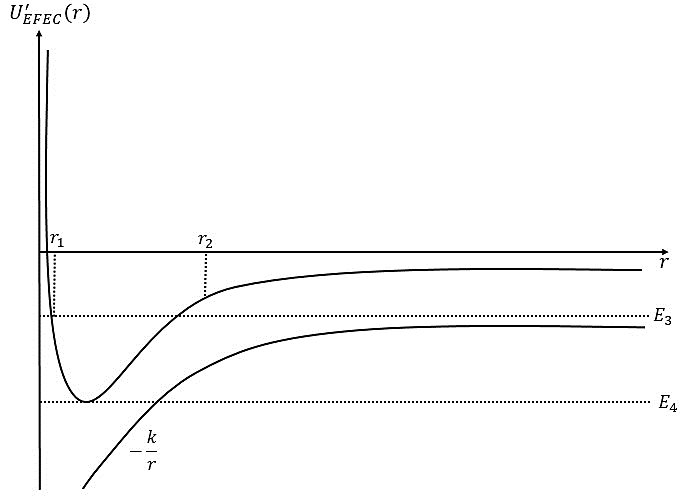
\includegraphics[width=6.03125in,height=4.3375in]{Imagenes/media/image53.png}

\[- \frac{\partial U_{EFEC}^{'}(r)}{\partial r} = {\overrightarrow{F}}_{EFEC}^{'}(r) = 0 = - \frac{\partial U}{\partial r} + \mu r{\dot{\phi}}^{2}\]

\[\frac{\partial U}{\partial r} = \mu r{\dot{\phi}}^{2}\]

Ahora analícese la forma que toman los ejes mayor y menor cuando la
órbita es una elipse.

El eje mayor de la elipse es la semisuma o media aritmética de las
distancias absidales.

\[a = {(r}_{1} + r_{2})/2\]

, si \(\phi_{0} = 0\), la distancia se comienza a medir a partir de
\(r_{1}\), donde \(r_{1}\) es un mínimo y \(r_{2}\) es un máximo.

, si \(r\) es un mínimo, \(\cos\phi\) es un máximo. \(\phi = 0\).

,

si \(r\) es máximo, \(\cos\phi\) es un mínimo. \(\phi = \pi\).

De esta manera:

\[\frac{\alpha}{r_{2}} = 1 - \epsilon\]

\[r_{1} = \frac{\alpha}{1 + \epsilon}\]

\[r_{2} = \frac{\alpha}{1 - \epsilon}\]

Luego:

\[a = \frac{\ \alpha}{2(1 + \epsilon)} + \frac{\ \alpha}{2(1 - \epsilon)}\]

\[a = \frac{\alpha(1 - \epsilon + 1 + \epsilon)}{2(1 + \epsilon)(1 - \epsilon)}\]

\[a = \frac{\alpha}{1 - \epsilon^{2}}\]

Sustituyendo:

\[a = \frac{\frac{l^{2}}{k\mu}}{1 - \left( 1 + \frac{2l^{2}}{\mu k^{2}}E \right)}\]

\[a = \frac{\frac{l^{2}}{k\mu}}{\frac{2l^{2}}{\mu k^{2}}|E|}\]

\[\mathbf{a =}\frac{\mathbf{k}}{\mathbf{2}\left| \mathbf{E} \right|}\]

La expresión (111) indica que el semieje mayor está relacionado con la
energía, es función de la energía, este es un teorema importante para la
teoría atómica de Bohr.

Ahora se procede a encontrar el periodo de oscilación de un planeta:

\[\frac{dA}{dt} = \frac{1}{2}r^{2}\frac{d\phi}{dt} = \frac{l}{2\mu}\]

\[\int_{0}^{A}{dA = \int_{0}^{\tau}{\frac{l}{2\mu}dt}}\]

De donde se tiene que:

\[\tau = \frac{2\mu}{l}A\]

\[\tau = \frac{2\mu}{l}\pi ab\]

Luego, para una elipse se cumple que:

\[b = \sqrt{1 - \epsilon^{2}}a = \sqrt{\frac{\alpha}{a}}a\]

De esta manera:

\[\tau = \frac{2\mu}{l}\pi a\sqrt{\frac{\alpha}{a}}a = \frac{2\mu}{l}\pi\sqrt{\frac{a^{4}\alpha}{a}} = \frac{2\mu}{l}\pi\sqrt{a^{3}\alpha}\]

\[\tau^{2} = \frac{4\mu^{2}\pi^{2}}{l^{2}}\alpha a^{3} = \frac{4\mu^{2}\pi^{2}}{l^{2}}\frac{l^{2}}{\mu k}a^{3}\]

\[\mathbf{\tau}^{\mathbf{2}}\mathbf{=}\frac{\mathbf{4}\mathbf{\mu}\mathbf{\pi}^{\mathbf{2}}}{\mathbf{k}}\mathbf{a}^{\mathbf{3}}\]

La expresión (112) corresponde la tercera Ley de Kepler. Si se tiene una
fuerza que está dada por:

\[\overrightarrow{F} = - G\frac{m_{1}m_{2}}{r^{2}}\widehat{a_{r}}\]

Se puede hallar el periodo de oscilación de cualquier planeta alrededor
del sol donde \(k = Gm_{1}m_{2}\):

\[\overrightarrow{F} = - \frac{k}{r^{2}}\]

De esta manera:

\[\tau^{2} = \frac{4\frac{m_{1}m_{2}}{m_{1} + m_{2}}}{Gm_{1}m_{2}}\pi^{2}a^{3}\]

\[\mathbf{\tau}^{\mathbf{2}}\mathbf{=}\frac{\mathbf{4}\mathbf{\pi}^{\mathbf{2}}}{\mathbf{G}\left( \mathbf{m}_{\mathbf{1}}\mathbf{+}\mathbf{m}_{\mathbf{2}} \right)}\mathbf{a}^{\mathbf{3}}\]

Si se asume \(m_{2}\) como la masa el sol, entonces \(m_{1} \ll m_{2}.\)

\textbf{Ejemplo 9:} Una masa \(m\) se mueve en una órbita circular bajo
la influencia de una fuerza cuyo potencial es \(- \frac{km}{r^{n}}\).
Mostrar que la órbita es estable para oscilaciones pequeñas, esto es, la
masa podría oscilar alrededor de la órbita circular.

\textbf{Solución:}

Pártase del potencial:

\[V_{r} = V(r) + \frac{{l\text{~}}^{2}}{2\mu r^{2}}\]

Gráficamente la situación se puede ver de la siguiente forma:

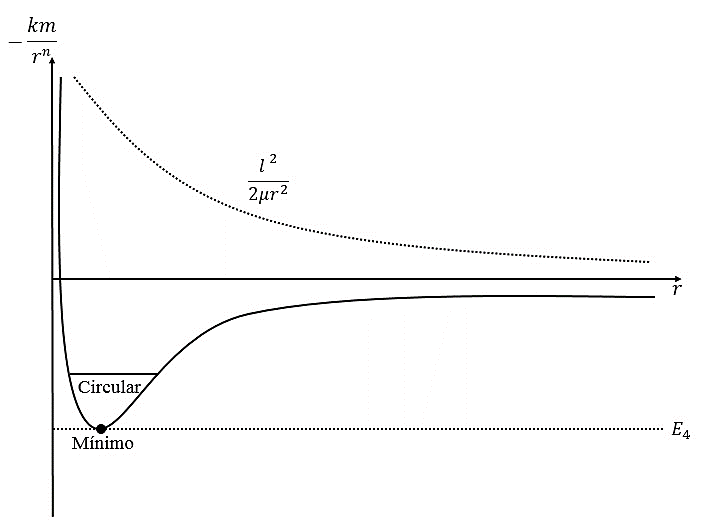
\includegraphics[width=6.36768in,height=4.73958in]{Imagenes/media/image54.png}

La primera condición matemática debe ser la condición de mínimo, dada
por:

\[\left. \ \frac{\partial V_{EFEC}^{'}(r)}{\ \partial r} \right\rfloor_{r_{0}} = 0\]

La curva potencial es efectiva y cóncava hacia arriba. La segunda
condición matemática es la que da estabilidad a la órbita.

Está dada por:

\[\frac{\partial^{2}V_{EFEC}^{'}(r)}{\partial r^{2}} > 0\]

Ahora teniendo en cuenta la información del planteamiento se tiene que:

\[V_{EFEC}^{'}(r) = - \frac{km}{r^{n}} + \frac{{l\text{~}}^{2}}{2\mu r^{2}}\]

\[{\overrightarrow{F}}_{EFEC}^{'}(r) = - \frac{\partial V_{EFEC}^{'}(r)}{\partial r}\]

Sustituyendo:

\[{\overrightarrow{F}}_{EFEC}^{'}(r) = - \frac{kmn}{r^{n + 1}} + \frac{{l\text{~}}^{2}}{\mu r^{3}} = 0\]

\[\frac{\partial^{2}V_{EFEC}^{'}(r)}{\partial r^{2}} = \frac{kmn(n + 1)}{r^{n + 2}} - \frac{3{l\text{~}}^{2}}{\mu r^{4}} > 0\]

\[\frac{kmn}{r^{n + 1}} = \frac{{l\text{~}}^{2}}{\mu r^{3}}\]

Reescribiendo:

\[\frac{kmn(n + 1)}{r^{n + 2}} - \frac{3}{r}\left( \frac{{l\text{~}}^{2}}{\mu r^{3}} \right) > 0\]

\[\frac{kmn(n + 1)}{r^{n + 2}} - \frac{3}{r}\left( \frac{kmn}{r^{n + 1}} \right) > 0\]

\[- \frac{kmn}{r^{n + 2}}\left\lbrack 3 - (n + 1) \right\rbrack > 0\]

\[3 - n - 1 > 0\]

\[2 > n\]

\[\mathbf{n < 2}\]

Por lo tanto queda demostrado que para oscilaciones pequeñas la órbita
es estable, ya que \(n < 2\).

\textbf{Ejemplo 10:} Una partícula de masa \(m\) se mueve en una órbita
circular de radio \(R\). La fuerza central yace en un punto \(C\). ¿Cuál
es la ley de interacción \(\overrightarrow{F}\)?

\textbf{Solución:} Obsérvese el esquema mostrado en la \emph{figura 38:}

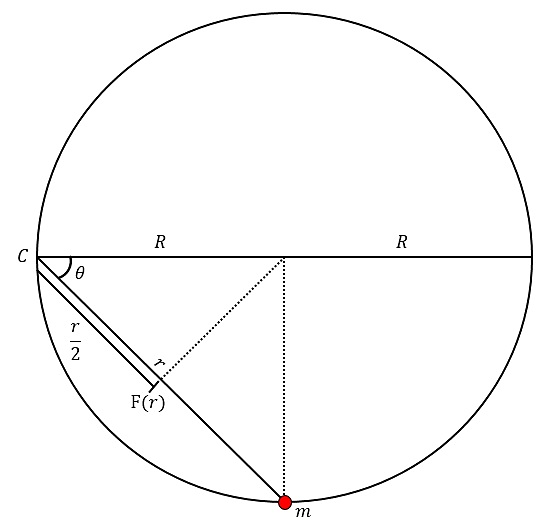
\includegraphics[width=5.35486in,height=5.01042in]{Imagenes/media/image55.png}

Inicialmente se tiene que:

\[\cos{\theta = \frac{\frac{r}{2}}{\frac{R}{1}}}\]

Es decir:

\[r = 2Rcos\ \theta\ \ \ \ \ \ \ \ \ \ \ \ \ \ \ \ trayectoria\ de\ la\ partícula\]

Ahora, utilizando la ecuación diferencial para el tipo de órbita se
tiene que:

\[U = \frac{1}{2RCos\ \theta} = \frac{1}{2R}{\cos\theta}^{- 1}\]

De esta manera:

\[\frac{dU}{d\theta} = - \frac{1}{2R}{\cos\theta}^{- 2}( - sen\ \theta)\]

\[\frac{dU}{d\theta} = \frac{sen\ \theta}{2R}{\cos\theta}^{- 2}\]

\[\frac{d^{2}U}{{d\theta}^{2}} = \frac{cos\ \theta}{2R\cos^{2}\theta} - \frac{2sen\ \theta{\cos\theta}^{- 3}( - sen\ \theta)}{2R}\]

\[\frac{d^{2}U}{{d\theta}^{2}} = \frac{cos\ \theta}{2R\cos^{2}\theta} + \frac{2{sen}^{2}\ \theta}{2R\cos^{3}\theta}\]

\[\frac{d^{2}U}{{d\theta}^{2}} = \frac{1}{2R}\left( \frac{1}{Cos\ \theta} + \frac{{2sen}^{2}\ \theta}{\cos^{3}\theta} \right)\]

Luego, sea:

\[\frac{d^{2}U}{{d\theta}^{2}} = \frac{1}{2R}\frac{\cos^{2}\theta + 2{sen}^{2}\ \theta}{\cos^{3}\theta}\]

\[\frac{d^{2}U}{{d\theta}^{2}} = \frac{1}{2R}\left( \frac{1 - {sen}^{2}\theta + 2{sen}^{2}\ \theta}{\cos^{3}\theta} \right)\]

Por lo tanto:

\[\frac{d^{2}u}{d\phi^{2}} + u = - \frac{\mu}{l^{2}}\left( \frac{1}{u^{2}} \right)F(u)\]

\[\frac{1}{2R}\left( \frac{1 - {sen}^{2}\theta + 2{sen}^{2}\ \theta}{\cos^{3}\theta} \right) + \frac{1}{2RCos\ \theta} = - \frac{\mu r^{2}}{l^{2}}F(r)\]

\[\frac{1}{2R}\left( \frac{1 + {sen}^{2}\theta + \cos^{2}\ \theta}{\cos^{3}\theta} \right) = - \frac{\mu r^{2}}{l^{2}}F(r)\]

\[\frac{1}{R\cos^{3}\theta} = - \frac{\mu r^{2}}{l^{2}}F(r)\]

Así mismo se tiene que:
\(r = 2Rcos\ \theta\ \ \ \ \ \ \ \ \ \ \ \ \ \ \ \ \)

\[\cos^{3}\theta = \frac{r^{3}}{8R^{3}}\]

Finalmente, la ley de interacción \(\overrightarrow{F}\) es entonces:

\[\mathbf{F}\left( \mathbf{r} \right)\mathbf{= -}\frac{\mathbf{8}{l^{2}\mathbf{R}}^{\mathbf{2}}}{\mathbf{\mu}}\left( \frac{\mathbf{1}}{\mathbf{r}^{\mathbf{5}}} \right)\]

\textbf{Capítulo 4 Teoría de Dispersión y Choques Elásticos}

En este capítulo se va a abordar lo que corresponde a la desintegración
espontánea de partículas donde se tiene una masa \(m\) que luego de una
interacción se convierte en dos masas \(m_{1}\) y \(m_{2}\); para que la
desintegración sea espontánea, la partícula de masa \(m\) debe estar
aislada. Algunas veces en esta temática es posible obtener conclusiones
de mucha importancia con respecto a una gran variedad de propiedades de
procesos mecánicos con tan sólo usar los teoremas de conservación de
momento lineal y de energía. Es de considerar que dichas propiedades no
dependen del tipo de interacción de las partículas que interactúan en el
proceso.

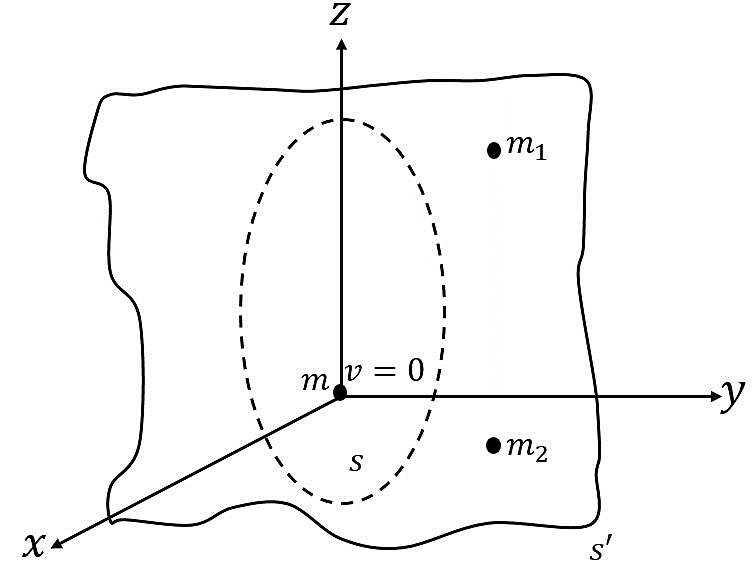
\includegraphics[width=6.04375in,height=4.58333in]{Imagenes/media/image56.png}En
primer lugar, tómese el caso de la desintegración espontánea de una
partícula que se convierte en otras dos partículas que se mueven de
manera independiente después de la desintegración. Este proceso tiene
una descripción más sencilla si se considera un sistema de referencia en
el cuál la partícula está en reposo antes de la desintegración tal como
se muestra en la \emph{figura 39:}

Para la descripción física de este proceso, pártase del teorema de
conservación de momento lineal, por lo que antes de la desintegración se
da que:

\[{\overrightarrow{p}}_{i} = 0\]

Asimismo, después de la desintegración:

\[{\overrightarrow{p}}_{2f} + {\overrightarrow{p}}_{2f} = cte\]

Por lo que:

\[{\overrightarrow{p}}_{1f} = - \ {\overrightarrow{p}}_{2f}\]

Las partículas que aparecen después de la desintegración tienen la misma
magnitud del momento pero viajan en direcciones opuestas. Para encontrar
la norma del momento lineal que tienen las dos partículas después de la
desintegración espontánea, se debe escribir el teorema de conservación
de la energía, esto es:

\[E_{i} = E_{if}\]

Donde \(E_{i}\) corresponde a la energía interna antes de la
desintegración de \(m\) y \(E_{if}\) corresponde a la energía interna
después de la desintegración para \(m_{1}\) y \(m_{2}\), de esta forma:

\[E_{i} = E_{i1} + T_{1} + E_{i2} + T_{2} = E_{i1} + \frac{1}{2}m_{1}v_{1}^{\ 2} + E_{i2} + \frac{1}{2}m_{2}v_{2}^{\ 2}\]

\[E_{i} - E_{i1} - E_{i2} = \frac{1}{2}\frac{\left( m_{1}v_{1} \right)^{2}}{m_{1}} + \frac{1}{2}\frac{\left( m_{2}v_{2} \right)^{2}}{m_{2}}\]

Para que la desintegración ocurra, la energía de desintegración
\(\epsilon = E_{i} - E_{i1} - E_{i2} > 0,\) así, la ecuación (115) toma
la forma:

\[\epsilon = \frac{1}{2}\frac{p_{1}^{\ 2}}{m_{1}} + \frac{1}{2}\frac{p_{2}^{\ 2}}{m_{2}}\]

Por el teorema de conservación de momento lineal:

\[p_{1} = - \ p_{2} = p_{0}\]

De esta manera la expresión (116) se puede escribir como:

\[\epsilon = \frac{1}{2}\frac{p_{0}^{\ 2}}{m_{1}} + \frac{1}{2}\frac{p_{0}^{\ 2}}{m_{2}} = \frac{p_{0}^{\ 2}}{2}\left( \frac{1}{m_{1}} + \frac{1}{m_{2}} \right) = \frac{p_{0}^{\ 2}}{2}\left( \frac{m_{2} + m_{1}}{m_{1}m_{2}} \right)\]

\[\epsilon\mathbf{=}\frac{\mathbf{p}_{\mathbf{0}}^{\mathbf{\ 2}}}{\mathbf{2}\mathbf{\mu}}\mathbf{\ \ \ \ \ \ \ \ \ \ \ \ }\]

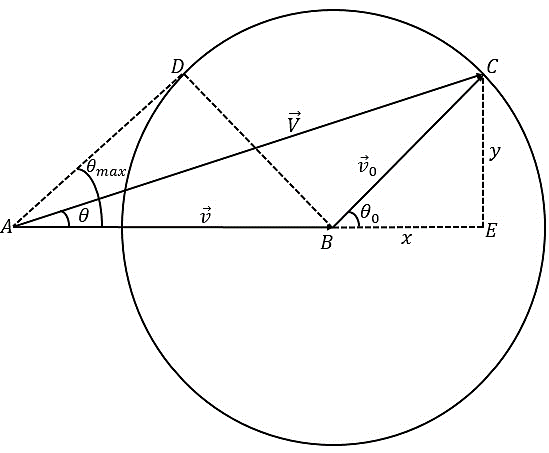
\includegraphics[width=3.78681in,height=3.25in]{Imagenes/media/image57.png}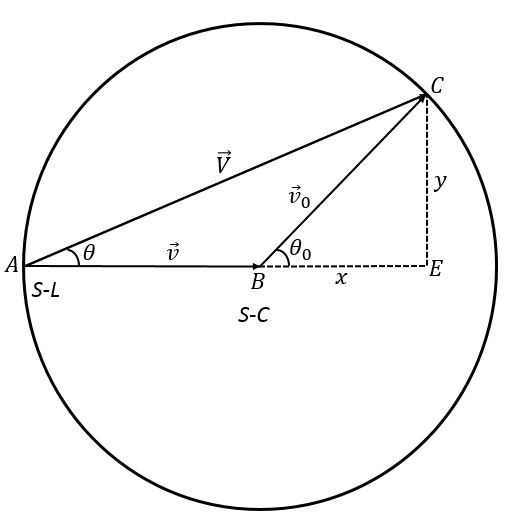
\includegraphics[width=3.28125in,height=3.3125in]{Imagenes/media/image58.jpeg}Ahora
se va a analizar la forma que toman las ecuaciones anteriores para un
sistema de observación donde la partícula de masa \(m\) (antes de la
desintegración) tiene una velocidad \(\overrightarrow{v}\) diferente de
cero, este sistema es denominado SISTEMA DE LABORATORIO (S-L), para esto
considérense los casos mostrados en las \emph{figuras 40} y \emph{41}:

En la \emph{figura 40} \(\overrightarrow{v} < {\overrightarrow{v}}_{0}\)
y la partícula puede viajar hacia la derecha; y en la \emph{figura 41}
\(\overrightarrow{v} > {\overrightarrow{v}}_{0}\) y la partícula viaja
hacia adelante, para cualquiera de los dos casos se analiza el triángulo
rectángulo \(ACE\), de donde:

\[\overrightarrow{V} = \overrightarrow{v} + {\overrightarrow{v}}_{0}\]

\[\overrightarrow{(v} + {\overrightarrow{v}}_{0}).\left( \overrightarrow{v} + {\overrightarrow{v}}_{0} \right) = \overrightarrow{V}.\overrightarrow{V}\]

\[V^{2} = v_{0}^{\ 2} + v^{2} + 2v_{0}v\cos\theta_{0}\]

\({\overrightarrow{v}}_{0}.{\overrightarrow{v}}_{0}\)=\(\overrightarrow{(V} - \overrightarrow{v}).\overrightarrow{(V} - \overrightarrow{v})\)

\[v_{0}^{\ 2} = V^{2} + v^{2} - 2Vv\cos\theta_{}\]

\[\tan{\theta = \frac{y}{v + x}}\]

Para conocer \(x\) e \(y\) se tiene, analizando el triángulo \(BCE\),
que:

\[{sen}\theta_{0} = \frac{y}{v_{0}} \rightarrow y = v_{0}{sen}\theta_{0}\]

\[\cos\theta_{0} = \frac{x}{v_{0}} \rightarrow x = v_{0}\cos\theta_{0}\]

De esta manera:

\[\tan\theta = \frac{v_{0}{sen}\theta_{0}}{v + v_{0}\cos\theta_{0}} = \frac{{sen}\theta}{\cos\theta}\]

\[sen\ \theta\left( v + v_{0}\cos\theta_{0} \right) = v_{0}sen\ \theta_{0}\cos\theta\]

\[v{sen}\theta + v_{0}{sen}\theta\cos\theta_{0} = v_{0}\sqrt{1 - \cos^{2}\theta_{0}}\cos\theta\]

Elevando al cuadrado ambos lados de la expresión (119):

\[v^{2}{sen}^{2}\theta + 2v{v_{0}sen}^{2}\theta\cos\theta_{0} + v_{0}^{\ 2}{sen}^{2}\theta\cos^{2}\theta_{0} = v_{0}^{\ 2}\left( 1 - \cos^{2}\theta_{0} \right)\cos^{2}\theta\]

\[\frac{v^{2}}{v_{0}^{\ 2}}{sen}^{2}\theta + \frac{2v}{v_{0}}{sen}^{2}\theta\cos\theta_{0} + {sen}^{2}\theta\cos^{2}\theta_{0} - \cos^{2}\theta + \cos^{2}\theta_{0}\cos^{2}\theta = 0\]

\[\cos^{2}\theta_{0}\left( {sen}^{2}\theta + \cos^{2}\theta \right) + \frac{2v}{v_{0}}{sen}^{2}\theta\cos\theta_{0} + \frac{v^{2}}{v_{0}^{\ 2}}{sen}^{2}\theta - \cos^{2}\theta = 0\]

\[\cos^{2}\theta_{0} + \left( \frac{2v}{v_{0}}{sen}^{2}\theta \right)\cos\theta_{0} + \frac{v^{2}}{v_{0}^{\ 2}}{sen}^{2}\theta - \cos^{2}\theta = 0\ \ \ \ \ \ \ \ \]

La ecuación (120) corresponde a una ecuación cuadrática en términos de
\(\cos\theta_{0}\) donde se identifica que:

\[a = 1\ \ \ \ \ \ \ \ \ \ \ \ \ \ \ \ b = \frac{2v}{v_{0}}{sen}^{2}\theta\ \ \ \ \ \ \ \ \ \ \ \ c = \frac{v^{2}}{v_{0}^{\ 2}}{sen}^{2}\theta - \cos^{2}\theta\]

Usando la fórmula cuadrática:

\[\cos\theta_{0} = \frac{- \frac{2v}{v_{0}}{sen}^{2}\theta \pm \sqrt{\frac{4v^{2}}{v_{0}^{\ 2}}{sen}^{4}\theta - 4\left( \frac{v^{2}}{v_{0}^{\ 2}}{sen}^{2}\theta - \cos^{2}\theta \right)}}{2}\]

\[\cos\theta_{0} = - \frac{v}{v_{0}}{sen}^{2}\theta \pm \sqrt{\frac{v^{2}}{v_{0}^{\ 2}}{sen}^{2}\theta\left( {sen}^{2}\theta - 1 \right) + \cos^{2}\theta}\]

\[\cos\theta_{0} = - \frac{v}{v_{0}}{sen}^{2}\theta \pm \sqrt{\cos^{2}\theta\left( 1 - \frac{v^{2}}{v_{0}^{\ 2}}{sen}^{2}\theta \right)}\]

Finalmente:

\[\mathbf{\cos}\mathbf{\theta}_{\mathbf{0}}\mathbf{= -}\frac{\mathbf{v}}{\mathbf{v}_{\mathbf{0}}}\mathbf{sen}^{\mathbf{2}}\mathbf{\theta}\mathbf{\pm}\mathbf{\cos}\mathbf{\theta}\sqrt{\mathbf{1 -}\frac{\mathbf{v}^{\mathbf{2}}}{\mathbf{v}_{\mathbf{0}}^{\mathbf{\ 2}}}\mathbf{sen}^{\mathbf{2}}\mathbf{\theta}}\mathbf{\ \ \ \ \ \ \ \ \ \ \ \ \ \ \ \ \ }\]

También es de notar que:

\[{{sen}\theta}_{\max} = \frac{v_{0}}{v}\]

En física interesa estudiar los fenómenos de desintegración pero de
muchas partículas, por lo tanto, se va a analizar cómo es la
distribución de las partículas después de la desintegración con respecto
a sus direcciones, su energía, etc. En caso de que el sistema de
referencia sea el que se denomina SISTEMA DE MOMENTO CERO (S-C), la ley
de distribución estará relacionada con el ángulo, para esto; se tiene en
cuenta la \emph{figura 42}:

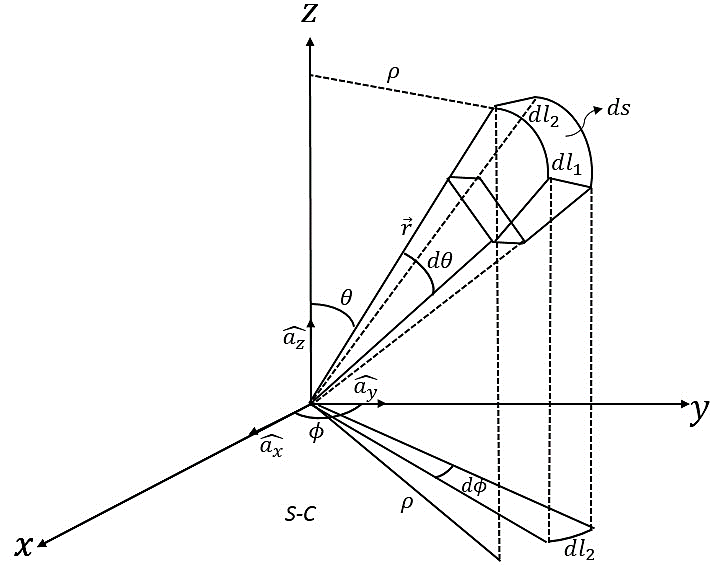
\includegraphics[width=5.15625in,height=4.07153in]{Imagenes/media/image59.png}

Se sabe que:

\[ds = dl_{1}dl_{2}\]

Donde:

\(dl_{1} = rd\theta\ \ \ \ \) y
\(dl_{2} = \rho d\phi = r{sen}\theta d\phi\)

De esta manera:

\[ds = r^{2}{sen}\theta_{0}d\theta_{0}d\phi\]

Introduciendo el ángulo sólido \(\Omega\), se da que:

\[\frac{ds}{r^{2}} = \int_{}^{}{d\Omega} = \int_{\theta_{0} = 0}^{\pi}{\int_{\phi = 0}^{2\pi}{{sen}\theta_{0}d\theta_{0}}d\phi} = \left. \ 2\pi\left( - \cos\theta_{0} \right) \right\rfloor_{0}^{\pi} = 4\pi\]

\[\mathbf{\Omega}\mathbf{= 4}\mathbf{\pi\ \ \ \ \ \ \ \ \ \ }\]

Del resultado (122) se puede establecer la relación
\(\frac{\Omega}{4\pi},\) la cual indica un valor promedio del número de
partículas dispersadas por unidad de ángulo sólido, de esta forma:

\[d\Omega = 2\pi{sen}\theta_{0}d\theta_{0}\]

\[\frac{d\Omega}{2\pi} = {sen}\theta_{0}d\theta_{0}\]

Multiplicando la expresión (123) por \(\frac{1}{2}:\)

\[\frac{\mathbf{d}\mathbf{\Omega}}{\mathbf{4}\mathbf{\pi}}\mathbf{=}{\frac{\mathbf{1}}{\mathbf{2}}\mathbf{sen}}\mathbf{\theta}_{\mathbf{0}}\mathbf{d}\mathbf{\theta}_{\mathbf{0}}\mathbf{\ \ \ \ \ \ \ \ \ \ }\]

La expresión (124) corresponde a la ley de dispersión que se refiere al
número de partículas contenidas en un elemento de ángulo sólido.

Ahora se va a estudiar cómo es la distribución con respecto a la energía
cinética de una de las partículas, esto respecto al sistema de
laboratorio S-L. Para este tratamiento, se retoman las \emph{figuras 40}
y \emph{41}, de donde se obtiene que:

\[\overrightarrow{V} = \overrightarrow{v} + {\overrightarrow{v}}_{0}\]

\[\overrightarrow{(v} + {\overrightarrow{v}}_{0}).\left( \overrightarrow{v} + {\overrightarrow{v}}_{0} \right) = \overrightarrow{V}.\overrightarrow{V}\]

\[V^{2} = v_{0}^{\ 2} + v^{2} + 2v_{0}v\cos\theta_{0}\]

\({\overrightarrow{v}}_{0}.{\overrightarrow{v}}_{0}\)=\(\overrightarrow{(V} - \overrightarrow{v}).\overrightarrow{(V} - \overrightarrow{v})\)

\[v_{0}^{\ 2} = V^{2} + v^{2} - 2Vv\cos\theta_{}\]

Derivando (125) con respecto a \(\cos\theta_{0}\), se tiene que:

\[\frac{dV^{2}}{d\cos\theta_{0}} = 2v_{0}v\]

\[\frac{dV^{2}}{2v_{0}v} = d\cos\theta_{0} = - {sen}\theta_{0}d\theta_{0}\]

Introduciendo la energía cinética a los cálculos se da que:

\[T = \frac{1}{2}m_{1}V^{2} \rightarrow dT\  = \frac{1}{2}m_{1}dV^{2} \rightarrow dV^{2} = \frac{2}{m_{1}}dT\]

\[\frac{1}{2v_{0}v}\frac{2}{m_{1}}dT = - {sen}\theta_{0}d\theta_{0}\]

\[\frac{\mathbf{1}}{\mathbf{2}}\frac{\mathbf{dT}}{\mathbf{m}_{\mathbf{1}}\mathbf{v}_{\mathbf{0}}\mathbf{V}}\mathbf{= -}\frac{\mathbf{1}}{\mathbf{2}}\mathbf{sen}\mathbf{\theta}_{\mathbf{0}}\mathbf{d}\mathbf{\theta}_{\mathbf{0}}\mathbf{\ \ \ \ \ \ \ \ \ \ \ \ \ }\]

La expresión (125) corresponde a la ley de dispersión de la energía
cinética con respecto al sistema S-L.

A continuación se va a encontrar la ley de dispersión de las partículas
con respecto a su dirección en el sistema de laboratorio.

\uline{Caso I:} \(\overrightarrow{v} < {\overrightarrow{v}}_{0}\)

Para este caso se parte del resultado obtenido en (121), esto es:

\[\cos\theta_{0} = - \frac{v}{v_{0}}{sen}^{2}\theta \pm \cos\theta\sqrt{1 - \frac{v^{2}}{v_{0}^{\ 2}}{sen}^{2}\theta}\]

\[\frac{1}{2}\frac{d}{d\theta}\left( \cos\theta_{0} \right) = \frac{1}{2}\frac{d}{d\theta}\left( - \frac{v}{v_{0}}{sen}^{2}\theta \pm \cos\theta\sqrt{1 - \frac{v^{2}}{v_{0}^{\ 2}}{sen}^{2}\theta} \right)\]

\[0 = - \frac{1}{2}{sen}\theta d\theta\left( 2\frac{v}{v_{0}}\cos\theta + \sqrt{1 - \frac{v^{2}}{v_{0}^{\ 2}}{sen}^{2}\theta} + \frac{v^{2}\cos^{2}\theta}{v_{0}^{\ 2}\sqrt{1 - \frac{v^{2}}{v_{0}^{\ 2}}{sen}^{2}\theta}} \right)\]

\[0 = \frac{1}{2}{sen}\theta d\theta\left( 2\frac{v}{v_{0}}\cos\theta + \frac{v_{0}^{\ 2}\left( 1 - \frac{v^{2}}{v_{0}^{\ 2}}{sen}^{2}\theta \right){` + v}^{2}\cos^{2}\theta}{v_{0}^{\ 2}\sqrt{1 - \frac{v^{2}}{v_{0}^{\ 2}}{sen}^{2}\theta}} \right)\]

Como \(\cos^{2}\theta - {sen}^{2}\theta = \cos{2\theta}\), entonces:

\[0 = \frac{1}{2}{sen}\theta d\theta\left( 2\frac{v}{v_{0}}\cos\theta + \frac{v^{2}\cos{2\theta} + v_{0}^{\ 2}}{v_{0}^{\ 2}\sqrt{1 - \frac{v^{2}}{v_{0}^{\ 2}}{sen}^{2}\theta}} \right)\]

\[\mathbf{0 =}\frac{\mathbf{1}}{\mathbf{2}}\mathbf{sen}\mathbf{\theta}\mathbf{d\theta}\left( \mathbf{2}\frac{\mathbf{v}}{\mathbf{v}_{\mathbf{0}}}\mathbf{\cos}\mathbf{\theta}\mathbf{+}\frac{\mathbf{1 +}\frac{\mathbf{v}^{\mathbf{2}}}{\mathbf{v}_{\mathbf{0}}^{\mathbf{\ 2}}}\mathbf{\cos}{\mathbf{2}\mathbf{\theta}}}{\sqrt{\mathbf{1 -}\frac{\mathbf{v}^{\mathbf{2}}}{\mathbf{v}_{\mathbf{0}}^{\mathbf{\ 2}}}\mathbf{sen}^{\mathbf{2}}\mathbf{\theta}}} \right)\mathbf{\ \ \ \ \ \ \ \ \ \ \ \ \ \ }\]

\[0 \leq \theta \leq \pi\]

\uline{Caso II:} \(\overrightarrow{v} > {\overrightarrow{v}}_{0}\)

Análogamente al caso anterior, se tiene que:

\[\cos\theta_{0} = - \frac{v}{v_{0}}{sen}^{2}\theta \pm \cos\theta\sqrt{1 - \frac{v^{2}}{v_{0}^{\ 2}}{sen}^{2}\theta}\]

\[0 = \frac{1}{2}{sen}\theta d\theta\left( - 2\frac{v}{v_{0}}\cos\theta + \frac{v^{2}\left( \cos^{2}\theta - {sen}^{2}\theta \right) + v_{0}^{\ 2}}{v_{0}^{\ 2}\sqrt{1 - \frac{v^{2}}{v_{0}^{\ 2}}{sen}^{2}\theta}} \right)\]

\[\mathbf{0 =}\frac{\mathbf{1}}{\mathbf{2}}\mathbf{sen}\mathbf{\theta}\mathbf{d\theta}\left( \mathbf{- 2}\frac{\mathbf{v}}{\mathbf{v}_{\mathbf{0}}}\mathbf{\cos}\mathbf{\theta}\mathbf{+}\frac{\mathbf{1 +}\frac{\mathbf{v}^{\mathbf{2}}}{\mathbf{v}_{\mathbf{0}}^{\mathbf{\ 2}}}\mathbf{\cos}{\mathbf{2}\mathbf{\theta}}}{\sqrt{\mathbf{1 -}\frac{\mathbf{v}^{\mathbf{2}}}{\mathbf{v}_{\mathbf{0}}^{\mathbf{\ 2}}}\mathbf{sen}^{\mathbf{2}}\mathbf{\theta}}} \right)\mathbf{\ \ \ \ \ \ \ \ \ \ \ \ \ \ }\]

Sumando las expresiones (126) y (127):

\[0 = \frac{1}{2}{sen}\theta d\theta\left( 2\frac{v}{v_{0}}\cos\theta + \frac{1 + \frac{v^{2}}{v_{0}^{\ 2}}\cos{2\theta}}{\sqrt{1 - \frac{v^{2}}{v_{0}^{\ 2}}{sen}^{2}\theta}} - 2\frac{v}{v_{0}}\cos\theta + \frac{1 + \frac{v^{2}}{v_{0}^{\ 2}}\cos{2\theta}}{\sqrt{1 - \frac{v^{2}}{v_{0}^{\ 2}}{sen}^{2}\theta}} \right)\ \ \ \ \ \ \ \ \ \ \ \ \ \ \]

\[0 = \frac{1}{2}{sen}\theta d\theta\left\lbrack 2\left( \frac{1 + \frac{V^{2}}{v_{0}^{\ 2}}\cos{2\theta}}{\sqrt{1 - \frac{V^{2}}{v_{0}^{\ 2}}{sen}^{2}\theta}} \right) \right\rbrack\ \ \ \ \ \ \ \ \ \ \ \ \ \ \]

\[\mathbf{0 =}\mathbf{sen}\mathbf{\theta}\mathbf{d\theta}\left( \frac{\mathbf{1 +}\frac{\mathbf{V}^{\mathbf{2}}}{\mathbf{v}_{\mathbf{0}}^{\mathbf{\ 2}}}\mathbf{\cos}{\mathbf{2}\mathbf{\theta}}}{\sqrt{\mathbf{1 -}\frac{\mathbf{V}^{\mathbf{2}}}{\mathbf{v}_{\mathbf{0}}^{\mathbf{\ 2}}}\mathbf{sen}^{\mathbf{2}}\mathbf{\theta}}} \right)\mathbf{\ \ \ \ \ \ \ \ \ \ \ \ \ \ }\]

caso II \(0 \leq \theta \leq \theta_{\max}\) con:

\[{sen}{\theta_{\max} =}\frac{v_{0}}{v}\]

A continuación se va a abordar la temática de choques elásticos,
recordando que un choque elástico o colisión elástica es aquella donde
no hay cambios de la energía interna del sistema, esto conlleva a que
las partículas no se puedan desintegrar, considérese el sistema mostrado
en la \emph{figura 43}:

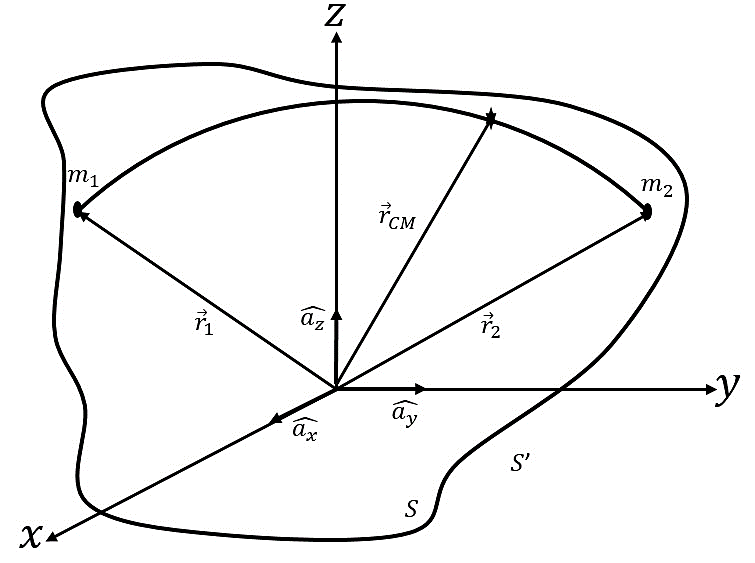
\includegraphics[width=5.57292in,height=4.15556in]{Imagenes/media/image60.png}

Para esto se tiene en cuenta que \(S\) no interactúa con \(S'\) y hay
conservación de momento lineal y de energía, por suma gráfica de
vectores, se tiene:

\[{\overrightarrow{r}}_{2} + \overrightarrow{r} = {\overrightarrow{r}}_{1}\]

\[\overrightarrow{r} = {\overrightarrow{r}}_{1} - {\overrightarrow{r}}_{2}\]

La ecuación (129) es la posición relativa de la partícula \(m_{1}\) con
respecto a la partícula \(m_{2}\), asimismo, el vector posición de
centro de masa es:

\[{\overrightarrow{r}}_{CM} = \frac{m_{1}{\overrightarrow{r}}_{1} + m_{2}{\overrightarrow{r}}_{2}}{m_{1} + m_{2}}\]

En primer lugar se procede a encontrar las velocidades de las partículas
\(m_{1}\) y \(m_{2}\) antes y después de la colisión con el sistema de
referencia centro de masa.

Para esto, se tiene que:

\[\left( m_{1} + m_{2} \right){\overrightarrow{r}}_{CM} = m_{1}{\overrightarrow{r}}_{1} + m_{2}\left( {\overrightarrow{r}}_{1} - \overrightarrow{r} \right)\]

\[\left( m_{1} + m_{2} \right){\overrightarrow{r}}_{CM} = \left( m_{1} + m_{2} \right){\overrightarrow{r}}_{1} - m_{2}\overrightarrow{r}\]

\[{\overrightarrow{\mathbf{r}}}_{\mathbf{1}}\mathbf{=}{\overrightarrow{\mathbf{r}}}_{\mathbf{CM}}\mathbf{+}\frac{\mathbf{m}_{\mathbf{2}}}{\mathbf{m}_{\mathbf{1}}\mathbf{+}\mathbf{m}_{\mathbf{2}}}\overrightarrow{\mathbf{r}}\]

Por otro lado:

\[\left( m_{1} + m_{2} \right){\overrightarrow{r}}_{CM} = m_{1}\left( {\overrightarrow{r}}_{2} + \overrightarrow{r} \right) + m_{2}{\overrightarrow{r}}_{2}\]

\[\left( m_{1} + m_{2} \right){\overrightarrow{r}}_{CM} = \left( m_{1} + m_{2} \right){\overrightarrow{r}}_{2} + m_{1}\overrightarrow{r}\]

\[{\overrightarrow{\mathbf{r}}}_{\mathbf{2}}\mathbf{=}{\overrightarrow{\mathbf{r}}}_{\mathbf{CM}}\mathbf{-}\frac{\mathbf{m}_{\mathbf{1}}}{\mathbf{m}_{\mathbf{1}}\mathbf{+}\mathbf{m}_{\mathbf{2}}}\overrightarrow{\mathbf{r}}\]

En el S-C \({\overrightarrow{r}}_{CM}\) se convierte en una coordenada
cíclica, es decir; no aparece en el Lagrangiano.
\({\overrightarrow{r}}_{cm} = 0\)

De esta manera las velocidades de \(m_{1}\) y \(m_{2}\) antes de la
colisión en el sistema S-C son:

\[{\overrightarrow{V}}_{10} = \frac{m_{2}}{m_{1} + m_{2}}\overrightarrow{V}\]

\[{\overrightarrow{V}}_{20} = - \frac{m_{1}}{m_{1} + m_{2}}\overrightarrow{V}\]

La velocidad relativa de la partícula \(m_{1}\) con respecto a la
velocidad de la partícula \(m_{2}\) es:

\[\overrightarrow{V} = {\overrightarrow{V}}_{1} - {\overrightarrow{V}}_{2}\]

Después de la colisión y por los teoremas de conservación de momento
lineal y de energía, las partículas viajan con la misma norma de momento
en direcciones opuestas. Si se introduce un vector unitario
\(\widehat{n_{O}}\) en la dirección de movimiento después de la colisión
para cualquiera de las dos partículas, las ecuaciones (132) y (133)
toman la forma:

\[{\overrightarrow{V}}_{10}' = \frac{m_{2}}{m_{1} + m_{2}}\left| \overrightarrow{V} \right|\widehat{n_{O}}\]

\[{\overrightarrow{V}}_{20}^{'} = - \frac{m_{1}}{m_{1} + m_{2}}\left| \overrightarrow{V} \right|\widehat{n_{O}}\]

Las ecuaciones (134) y (135) son las velocidades de las partículas
\(m_{1}\) y \(m_{2}\) después de la colisión en el S-C.

Ahora se procede a analizar la forma que toman las expresiones de las
velocidades de las partículas en un sistema de referencia de laboratorio
(S-L), esto es:

\[{\overrightarrow{r}}_{1} = \frac{m_{1}{\overrightarrow{r}}_{1} + m_{2}{\overrightarrow{r}}_{2}}{m_{1} + m_{2}} + \frac{m_{2}}{m_{1} + m_{2}}\overrightarrow{r}\]

\[{\overrightarrow{r}}_{2} = \frac{m_{1}{\overrightarrow{r}}_{1} + m_{2}{\overrightarrow{r}}_{2}}{m_{1} + m_{2}} - \frac{m_{1}}{m_{1} + m_{2}}\overrightarrow{r}\]

Las velocidades de \(m_{1}\) y \(m_{2}\) antes de la colisión medidas en
el S-L van a estar dadas por:

\[{\overrightarrow{v}}_{1} = \frac{m_{1}{\overrightarrow{V}}_{1} + m_{2}{\overrightarrow{V}}_{2}}{m_{1} + m_{2}} + \frac{m_{2}}{m_{1} + m_{2}}\overrightarrow{V}\]

\[{\overrightarrow{v}}_{2} = \frac{m_{1}{\overrightarrow{V}}_{1} + m_{2}{\overrightarrow{V}}_{2}}{m_{1} + m_{2}} - \frac{m_{1}}{m_{1} + m_{2}}\overrightarrow{V}\]

Después de la colisión (136) y (137) toman la forma:

\[{\overrightarrow{v}}_{1}' = \frac{m_{1}{\overrightarrow{V}}_{1} + m_{2}{\overrightarrow{V}}_{2}}{m_{1} + m_{2}} + \frac{m_{2}}{m_{1} + m_{2}}\left| \overrightarrow{V} \right|\widehat{n_{O}}\]

\[{\overrightarrow{v}}_{2}' = \frac{m_{1}{\overrightarrow{V}}_{1} + m_{2}{\overrightarrow{V}}_{2}}{m_{1} + m_{2}} - \frac{m_{1}}{m_{1} + m_{2}}\left| \overrightarrow{V} \right|\widehat{n_{O}}\]

Ahora; haciendo una interpretación geométrica de las expresiones (138) y
(139), se tiene para el momento lineal de cada partícula que:

\[{\overrightarrow{p}}_{1}' = m_{1}{\overrightarrow{v}}_{1}^{\ \ '} = m_{1}\left( \frac{m_{1}{\overrightarrow{V}}_{1} + m_{2}{\overrightarrow{V}}_{2}}{m_{1} + m_{2}} \right) + \frac{m_{1}m_{2}}{m_{1} + m_{2}}\left| \overrightarrow{V} \right|\widehat{n_{O}}\]

\[{\overrightarrow{p}}_{2}' = m_{2}{\overrightarrow{v}}_{2}^{\ \ '} = m_{2}\left( \frac{m_{1}{\overrightarrow{V}}_{1} + m_{2}{\overrightarrow{V}}_{2}}{m_{1} + m_{2}} \right) - \frac{m_{1}m_{2}}{m_{1} + m_{2}}\left| \overrightarrow{V} \right|\widehat{n_{O}}\]

Introduciendo la masa reducida:

\[{\overrightarrow{p}}_{1}' = m_{1}\left( \frac{m_{1}{\overrightarrow{V}}_{1} + m_{2}{\overrightarrow{V}}_{2}}{m_{1} + m_{2}} \right) + \mu\left| \overrightarrow{V} \right|\widehat{n_{O}}\]

\[{\overrightarrow{p}}_{2}' = m_{2}\left( \frac{m_{1}{\overrightarrow{V}}_{1} + m_{2}{\overrightarrow{V}}_{2}}{m_{1} + m_{2}} \right) - \mu\left| \overrightarrow{V} \right|\widehat{n_{O}}\]

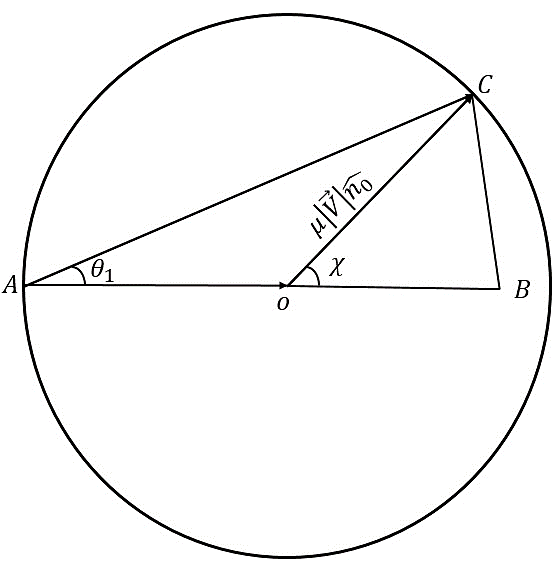
\includegraphics[width=3.77083in,height=3.79722in]{Imagenes/media/image61.png}Gráficamente,
esto es:

\(\chi\) representa el ángulo de desviación de la partícula \(m_{1}\)
después de la colisión en S-C.

\(\theta\) representa el ángulo de desviación de la partícula \(m_{1}\)
después de la colisión en S-L.

Se procede a probar:

\[\overrightarrow{AO} + \overrightarrow{OC} = \overrightarrow{AC}\]

\[\overrightarrow{AO} + \mu\left| \overrightarrow{V} \right|\widehat{n_{o}} = \overrightarrow{AC}\]

Es de identificar que:

\[\overrightarrow{AC} = {\overrightarrow{p}}_{1}'\ ,\ \ \ \ \ \ \ \ \ \overrightarrow{AO} = m_{1}\left( \frac{m_{1}{\overrightarrow{V}}_{1} + m_{2}{\overrightarrow{V}}_{2}}{m_{1} + m_{2}} \right)\]

De esta manera:

\[{\overrightarrow{\mathbf{p}}}_{\mathbf{1}}^{\mathbf{'}}\mathbf{=}\mathbf{m}_{\mathbf{1}}\left( \frac{\mathbf{m}_{\mathbf{1}}{\overrightarrow{\mathbf{V}}}_{\mathbf{1}}\mathbf{+}\mathbf{m}_{\mathbf{2}}{\overrightarrow{\mathbf{V}}}_{\mathbf{2}}}{\mathbf{m}_{\mathbf{1}}\mathbf{+}\mathbf{m}_{\mathbf{2}}} \right)\mathbf{+ \mu}\left| \overrightarrow{\mathbf{V}} \right|\widehat{\mathbf{n}_{\mathbf{O}}}\mathbf{\ \ \ \ \ \ \ \ \ \ \ }\]

Por otro lado:

\[\overrightarrow{OC} + \overrightarrow{CB} = \overrightarrow{OB}\]

\[\overrightarrow{CB} = \overrightarrow{OB} - \overrightarrow{OC}\]

Análogamente al caso anterior, se puede identificar que:

\[\overrightarrow{OC} = \mu\left| \overrightarrow{V} \right|\widehat{n_{o}},\ \ \ \ \ \ \ \ \ \ \overrightarrow{CB} = {\overrightarrow{p}}_{2}^{'}\ ,\ \ \ \ \ \ \ \ \ \ \ \overrightarrow{OB} = m_{2}\left( \frac{m_{1}{\overrightarrow{V}}_{1} + m_{2}{\overrightarrow{V}}_{2}}{m_{1} + m_{2}} \right)\]

Por lo tanto:

\[{\overrightarrow{\mathbf{p}}}_{\mathbf{2}}^{\mathbf{\ \ '}}\mathbf{=}\mathbf{m}_{\mathbf{2}}\left( \frac{\mathbf{m}_{\mathbf{1}}{\overrightarrow{\mathbf{V}}}_{\mathbf{1}}\mathbf{+}\mathbf{m}_{\mathbf{2}}{\overrightarrow{\mathbf{V}}}_{\mathbf{2}}}{\mathbf{m}_{\mathbf{1}}\mathbf{+}\mathbf{m}_{\mathbf{2}}} \right)\mathbf{- \mu}\left| \overrightarrow{\mathbf{V}} \right|\widehat{\mathbf{n}_{\mathbf{O}}}\mathbf{\ \ \ \ \ \ \ \ \ }\]

Ahora se va a analizar un caso donde la masa \(m_{2}\ \)se encuentra en
reposo, por lo tanto:

\[\overrightarrow{AO} = \frac{m_{1}\left( m_{1}{\overrightarrow{V}}_{1} \right)}{m_{1} + m_{2}}\]

\[\overrightarrow{OB} = \frac{m_{2}m_{1}{\overrightarrow{V}}_{1}}{m_{1} + m_{2}}\]

Sumando (144) y (145) se da que:

\[\overrightarrow{AO} + \overrightarrow{OB} = \overrightarrow{AB}\]

\[\overrightarrow{AB} = \frac{m_{1}\left( m_{1}{\overrightarrow{V}}_{1} \right)}{m_{1} + m_{2}} + \frac{m_{2}m_{1}{\overrightarrow{V}}_{1}}{m_{1} + m_{2}}\]

\[\overrightarrow{AB} = \frac{m_{1}{\overrightarrow{V}}_{1}\left( m_{1} + m_{2} \right)}{m_{1} + m_{2}}\]

\[\overrightarrow{\mathbf{AB}}\mathbf{=}\mathbf{m}_{\mathbf{1}}{\overrightarrow{\mathbf{V}}}_{\mathbf{1}}\mathbf{\ \ \ \ \ }\]

El resultado (146) corresponde al momento después de la colisión cuando
\(m_{2}\) se encuentra en reposo, es el mismo momento que tiene la
partícula \(m_{1}\) antes de la colisión.

Como \({\overrightarrow{v}}_{2} = 0\), entonces
\({\overrightarrow{v}}_{1} = \overrightarrow{V}\), asimismo
\(\overrightarrow{OB} = \mu\left| \overrightarrow{V} \right|\) lo que
implica que
\(\left| \overrightarrow{OB} \right| = \left| \overrightarrow{OC} \right|\).

El punto \(B\) se encuentra sobre la trayectoria del círculo máximo.

Ejercicio: Expresar en el sistema S-L las velocidades después del choque
de dos partículas de las cuáles la partícula \(m_{1}\) estaba en
movimiento y la partícula \(m_{2}\) en reposo, en función de sus
direcciones de movimiento. \(\therefore\)

A continuación se va a encontrar el ángulo de dispersión de la partícula
\(m_{1}\) después de la colisión en el S-L con respecto al ángulo
\(\chi\) del S-C, para esto se considera el siguiente diagrama:

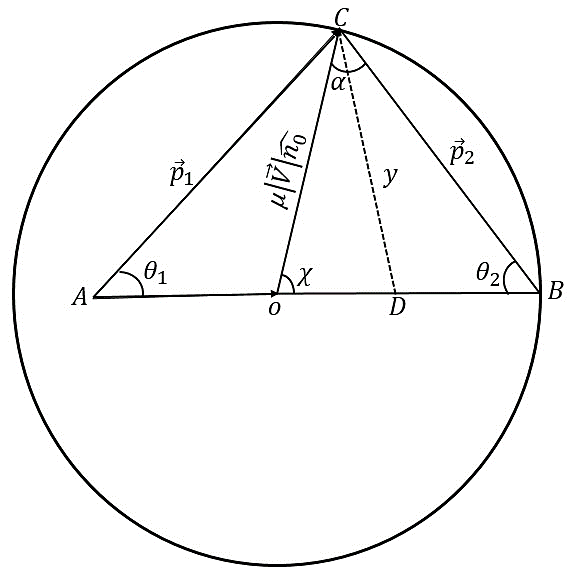
\includegraphics[width=4.42708in,height=4.45in]{Imagenes/media/image62.png}

Analizando el esquema anterior, del triángulo \(ACD\), se cumple que:

\[\tan\theta_{1} = \frac{y}{\overrightarrow{AO} + \overrightarrow{OD}}\]

Del triángulo \(OCD:\)

\[\cos\chi = \frac{\overrightarrow{OD}}{\mu\left| \overrightarrow{V} \right|},\ \ \ \ \ \ \ \ \ \ {sen}{\chi = \frac{y}{\mu\left| \overrightarrow{V} \right|}}\]

De esta manera (147) toma la forma:

\[\tan\theta_{1} = \frac{\frac{\mu\left| \overrightarrow{V} \right|sen\chi}{m_{1}\left( m_{1}\left| \overrightarrow{V_{1}} \right| + m_{2}\left| {\overrightarrow{V}}_{2} \right| \right)}}{m_{1} + m_{2}} + \mu\left| \overrightarrow{V} \right|\cos\chi\]

Si \(m_{2}\) se encuentra en reposo:

\[\tan\theta_{1} = \frac{\frac{\frac{m_{1}m_{2}}{m_{1} + m_{2}}\left| \overrightarrow{V} \right|sen\chi}{m_{1}\left( m_{1}\left| \overrightarrow{V_{1}} \right| + m_{1}m_{2}\left| \overrightarrow{V} \right|\cos\chi \right)}}{m_{1} + m_{2}}\]

\[\tan\theta_{1} = \frac{m_{1}m_{2}\left| \overrightarrow{V} \right|sen\chi}{m_{1}\left| \overrightarrow{V} \right|\left( m_{1} + m_{2}\cos\chi \right)}\]

\[\mathbf{\tan}\mathbf{\theta}_{\mathbf{1}}\mathbf{=}\frac{\mathbf{m}_{\mathbf{2}}\mathbf{sen\chi}}{\mathbf{m}_{\mathbf{1}}\mathbf{+}\mathbf{m}_{\mathbf{2}}\mathbf{\cos}\mathbf{\chi}}\mathbf{\ \ \ \ \ \ \ \ \ \ }\]

La expresión (149) corresponde al ángulo de dispersión de la partícula
\(m_{1}\) después de la colisión en el S-L con respecto al ángulo
\(\chi\) del S-C.

Como \(\overrightarrow{OC} = \overrightarrow{OB}\) el triángulo \(OCB\)
es un triángulo isósceles, por lo que:

\[\chi + \theta_{2} + \alpha = \pi\]

\[\chi + 2\theta_{2} = \pi\]

\[\mathbf{\theta}_{\mathbf{2}}\mathbf{=}\frac{\mathbf{\pi - \chi}}{\mathbf{2}}\mathbf{\ \ \ \ \ }\]

Por otro lado:

\[\frac{\left| \overrightarrow{AO} \right|}{\left| \overrightarrow{OB} \right|} = \frac{\frac{m_{1}\left( m_{1}\left| {\overrightarrow{V}}_{1} \right| + m_{2}\left| {\overrightarrow{V}}_{2} \right| \right)}{m_{1} + m_{2}}}{\frac{m_{2}\left( m_{1}\left| {\overrightarrow{V}}_{1} \right| + m_{2}\left| {\overrightarrow{V}}_{2} \right| \right)}{m_{1} + m_{2}}}\]

\[\frac{\left| \overrightarrow{AO} \right|}{\left| \overrightarrow{OB} \right|} = \frac{m_{1}}{m_{2}}\]

\[\left| \overrightarrow{AO} \right| = \frac{m_{1}}{m_{2}}\left| \overrightarrow{OB} \right|\]

Si
\(m_{1} < m_{2},\ \left| \overrightarrow{AO} \right| < \left| \overrightarrow{OB} \right|\)
y el punto \(A\) se encuentra dentro de la circunferencia; y si
\(m_{1} > m_{2}\),
\(\left| \overrightarrow{AO} \right| > \left| \overrightarrow{OB} \right|\)
el punto \(A\) se encuentra fuera de la circunferencia y:

\[\mathbf{sen}\mathbf{\theta}_{\mathbf{\max}}\mathbf{=}\frac{\mathbf{m}_{\mathbf{2}}}{\mathbf{m}_{\mathbf{1}}}\mathbf{\ \ \ \ \ \ \ }\]

Ahora se procede a encontrar las normas de los vectores de velocidad
para las partículas \(m_{1}\) y \(m_{2}\) después de la colisión en el
S-L con respecto al ángulo \(\chi\) del S-C, para esto se utiliza la
\emph{figura 46}:

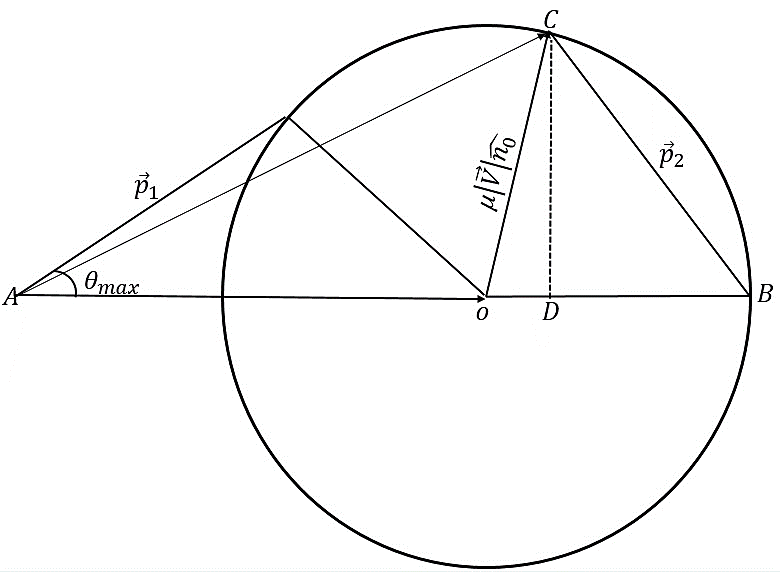
\includegraphics[width=5.25417in,height=3.83333in]{Imagenes/media/image63.png}

Del triángulo rectángulo \(ADC\), usando el teorema de Pitágoras, se
tiene que:

\[\left( \overline{AO} + \overline{OD} \right)^{2} + {\overline{DC}}^{2} = {\overline{AC}}^{2}\]

Como \(m_{2}\ \)se encuentra en reposo:

\[\overline{AO} = \frac{m_{1}^{\ 2}\left| \overrightarrow{V} \right|}{m_{1} + m_{2}}\]

\[\overline{OD} = \mu\left| \overrightarrow{V} \right|\cos\chi\]

\[\overline{DC} = \mu\left| \overrightarrow{V} \right|{sen}\chi\]

Llevando las expresiones anteriores a (150), se tiene que:

\[\left( \frac{m_{1}^{\ 2}\left| \overrightarrow{V} \right|}{m_{1} + m_{2}} + \frac{m_{1}m_{2}}{m_{1} + m_{2}}\left| \overrightarrow{V} \right|\cos\chi \right)^{2} + \left( \frac{m_{1}m_{2}}{m_{1} + m_{2}}\left| \overrightarrow{V} \right|{sen}\chi \right)^{2} = m_{1}{m_{1}\left| {\overrightarrow{v}}_{1}' \right|}^{2}\]

\[\frac{m_{1}^{\ 4}\left| \overrightarrow{V} \right|^{2}}{\left( m_{1} + m_{2} \right)^{2}} + \frac{2m_{1}^{\ \ 2}m_{1}m_{2}\left| \overrightarrow{V} \right|^{2}\cos\chi}{\left( m_{1} + m_{2} \right)^{2}} + \frac{m_{1}^{\ 2}{m_{2}^{\ \ 2}\left| \overrightarrow{V} \right|}^{2}\cos^{2}\chi}{\left( m_{1} + m_{2} \right)^{2}} + \frac{m_{1}^{\ \ 2}m_{2}^{\ \ 2}\left| \overrightarrow{V} \right|^{2}{sen}^{2}\chi}{\left( m_{1} + m_{2} \right)^{2}} = m_{1}m_{1}\left| {\overrightarrow{V}}_{1}' \right|^{2}\]

\[\frac{m_{1}^{\ \ 2}\left| \overrightarrow{V} \right|^{2} + 2m_{1}m_{2}\left| \overrightarrow{V} \right|^{2}\cos\chi + m_{2}^{\ \ 2}\left| \overrightarrow{V} \right|^{2}\cos^{2}\chi + m_{2}^{\ \ 2}\left| \overrightarrow{V} \right|^{2}{sen}^{2}\chi}{\left( m_{1} + m_{2} \right)^{2}} = \left| {\overrightarrow{v}}_{1}' \right|^{2}\]

\[\frac{\left| \overrightarrow{V} \right|^{2}\left\lbrack m_{1}^{\ \ 2} + m_{2}^{\ \ 2}\left( \cos^{2}\chi + {sen}^{2}\chi \right) \right\rbrack + 2m_{1}m_{2}\cos^{}{\chi\rbrack}}{\left( m_{1} + m_{2} \right)^{2}} = \left| {\overrightarrow{v}}_{1}' \right|^{2}\]

\[\frac{\left( m_{1}^{\ \ 2} + m_{2}^{\ \ 2} + 2m_{1}m_{2}\cos\chi \right)\left| \overrightarrow{V} \right|^{2}}{\left( m_{1} + m_{2} \right)^{2}} = \left| {\overrightarrow{v}}_{1}' \right|^{2}\]

Finalmente:

\[\left| {\overrightarrow{v}}_{1}' \right|\mathbf{=}\frac{\sqrt{\mathbf{m}_{\mathbf{1}}^{\mathbf{\ \ 2}}\mathbf{+}\mathbf{m}_{\mathbf{2}}^{\mathbf{\ \ 2}}\mathbf{+ 2}\mathbf{m}_{\mathbf{1}}\mathbf{m}_{\mathbf{2}}\mathbf{\cos}\mathbf{\chi}}}{\mathbf{m}_{\mathbf{1}}\mathbf{+}\mathbf{m}_{\mathbf{2}}}\left| \overrightarrow{\mathbf{V}} \right|\mathbf{\ \ \ \ \ \ \ \ \ \ \ \ }\]

Ahora se procede a analizar el triángulo rectángulo \(DCB\), por el
teorema de Pitágoras:

\[\left( \overline{OB} - \overline{OD} \right)^{2} + {\overline{DC}}^{2} = {\overline{CB}}^{2}\]

Donde cada segmento está dado por:

\[\overline{OB} = \frac{m_{1}m_{2}}{m_{1} + m_{2}}\left| \overrightarrow{V} \right|,\ \ \ \ \ \ \ \ \ \overline{OD} = \mu\left| \overrightarrow{V} \right|\cos\chi\]

\[\ \ \ \ \ \ \ \ \ \ \ \ \ \ \ \ \ \ \ \ \ \ \ \ \ \ \ \ \ \ \ \ \ \ \ \ \ \ \ \ \ \overline{DC} = \mu\left| \overrightarrow{V} \right|{sen}\chi,\ \ \ \ \ \ \ \ \overline{CB} = \left| {\overrightarrow{p}}_{2} \right|\ \ \ \ \ \ \ \ \ \ \ \ \ \ \ \ \ \ \ \ \ \ \ \ \ \ \ \ \ \ \ \ \ \ \ \ \ \ \ \ \ \ \ \ \ \ \ \]

Llevando las expresiones anteriores a (152):

\[\left( \frac{m_{1}m_{2}}{m_{1} + m_{2}}\left| \overrightarrow{V} \right| - \frac{m_{1}m_{2}}{m_{1} + m_{2}}\left| \overrightarrow{V} \right|\cos\chi \right)^{2} + \left( \frac{m_{1}m_{2}}{m_{1} + m_{2}}\left| \overrightarrow{V} \right|{sen}\chi \right)^{2} = m_{2}^{\ \ \ 2}\left| {\overrightarrow{v}}_{2}' \right|^{2}\]

\[\frac{m_{1}^{\ 2}m_{2}^{\ \ 2}\left| \overrightarrow{V} \right|^{2}}{\left( m_{1} + m_{2} \right)^{2}} - \frac{2m_{1}^{\ \ 2}m_{2}^{\ \ 2}\left| \overrightarrow{V} \right|^{2}\cos\chi}{\left( m_{1} + m_{2} \right)^{2}} + \frac{m_{1}^{\ 2}{m_{2}^{\ \ 2}\left| \overrightarrow{V} \right|}^{2}\cos^{2}\chi}{\left( m_{1} + m_{2} \right)^{2}} + \frac{m_{1}^{\ \ 2}m_{2}^{\ \ 2}\left| \overrightarrow{V} \right|^{2}{sen}^{2}\chi}{\left( m_{1} + m_{2} \right)^{2}} = m_{2}^{\ \ \ 2}\left| {\overrightarrow{v}}_{2}' \right|^{2}\]

Análogamente al caso anterior, el resultado que se tiene es:

\[\left| {\overrightarrow{v}}_{2}' \right| = \sqrt{\frac{{\left| \overrightarrow{V} \right|^{2}2m_{1}^{\ \ 2}}^{}\left( 1 - \cos\chi \right)}{\left( m_{1} + m_{2} \right)^{2}}}\]

Como \(1 - \cos\chi = 2{sen}^{2}\left( \frac{\chi}{2} \right)\), por lo
tanto:

\[\left| {\overrightarrow{v}}_{2}' \right|\mathbf{=}\frac{\mathbf{2}\mathbf{m}_{\mathbf{1}}\mathbf{sen}\left( \frac{\mathbf{\chi}}{\mathbf{2}} \right)}{\mathbf{m}_{\mathbf{1}}\mathbf{+}\mathbf{m}_{\mathbf{2}}}\left| \overrightarrow{\mathbf{V}} \right|\mathbf{\ \ \ \ \ \ \ \ \ \ \ \ \ }\]

Para el caso en que las dos partículas \(m_{1}\) y \(m_{2}\) tienen una
colisión directa, es decir, viajan a lo largo del segmento
\(\overline{AO}\) y por conservación de momento lineal, las dos
partículas viajan en direcciones opuestas, o sea \(\chi = \pi\), de este
modo:

\[\left| {\overrightarrow{v}}_{1}' \right| = \frac{\sqrt{m_{1}^{\ \ 2} + m_{2}^{\ \ 2} + 2m_{1}m_{2}\cos\pi}}{m_{1} + m_{2}}\left| \overrightarrow{V} \right|\]

\[\left| {\overrightarrow{v}}_{1}' \right| = \frac{\sqrt{m_{1}^{\ \ 2} + m_{2}^{\ \ 2} - 2m_{1}m_{2}}}{m_{1} + m_{2}}\left| \overrightarrow{V} \right|\]

\[\left| {\overrightarrow{v}}_{1}' \right| = \frac{\sqrt{\left( m_{1} - m_{2} \right)^{2}}}{m_{1} + m_{2}}\left| \overrightarrow{V} \right|\]

\[\left| {\overrightarrow{v}}_{1}' \right|\mathbf{=}\frac{\mathbf{m}_{\mathbf{1}}\mathbf{-}\mathbf{m}_{\mathbf{2}}}{\mathbf{m}_{\mathbf{1}}\mathbf{+}\mathbf{m}_{\mathbf{2}}}\left| \overrightarrow{\mathbf{V}} \right|\mathbf{\ \ \ \ \ \ \ \ \ }\]

Asimismo:

\[\left| {\overrightarrow{v}}_{2}' \right| = \frac{2m_{1}{sen}\left( \frac{\pi}{2} \right)}{m_{1} + m_{2}}\left| \overrightarrow{V} \right|\]

\[\left| {\overrightarrow{v}}_{2}' \right|\mathbf{=}\frac{\mathbf{2}\mathbf{m}_{\mathbf{1}}}{\mathbf{m}_{\mathbf{1}}\mathbf{+}\mathbf{m}_{\mathbf{2}}}\left| \overrightarrow{\mathbf{V}} \right|\mathbf{\ \ \ \ \ \ \ \ \ \ \ \ }\]

Como \({sen}\left( \frac{\pi}{2} \right)\) es máxima,
\(\left| {\overrightarrow{v}}_{2}' \right|\)es una velocidad máxima, por
lo que a partir del resultado (155) es posible hallar la energía máxima
de la colisión, esto es:

\[E_{2max}^{'} = \frac{1}{2}m_{2}\left| {\overrightarrow{v}}_{2}' \right|^{2} = \frac{1}{2}m_{2}\left\lbrack \frac{4m_{1}^{\ \ 2}}{\left( m_{1} + m_{2} \right)^{2}} \right\rbrack\left| \overrightarrow{V} \right|^{2}\]

Antes de la colisión hay energía de la partícula \(m_{1}\), por lo que:

\[E_{1} = \frac{1}{2}m_{1}\left| {\overrightarrow{v}}_{1} \right|^{2} \rightarrow 2E_{1} = m_{1}\left| {\overrightarrow{v}}_{1} \right|^{2}\]

\[E_{2max}^{'} = \frac{1}{2}\frac{m_{2}4m_{1}}{\left( m_{1} + m_{2} \right)^{2}}\left( m_{1}\left| \overrightarrow{V} \right|^{2} \right)\]

\[E_{2max}^{'} = \frac{1}{2}\frac{m_{2}4m_{1}}{\left( m_{1} + m_{2} \right)^{2}}2E_{1}\]

\[\mathbf{E}_{\mathbf{2}\mathbf{\max}}^{\mathbf{'}}\mathbf{=}\frac{\mathbf{4}\mathbf{\mu}}{\mathbf{m}_{\mathbf{1}}\mathbf{+}\mathbf{m}_{\mathbf{2}}}\mathbf{E}_{\mathbf{1}}\mathbf{\ \ \ \ \ \ \ \ \ \ }\]

Ahora, se va a analizar el caso en que \(m_{2}\) se encuentra en reposo
cuando \(m_{1} = m_{2}\), de esta manera:

\[\overline{AO} = \frac{m_{1}\left( m_{1}\left| {\overrightarrow{V}}_{1} \right| + m_{2}\left| {\overrightarrow{V}}_{2} \right| \right)}{m_{1} + m_{2}},\ \ \ \ \ \ \ \ \ \overline{OB} = \frac{m_{2}\left( m_{1}\left| {\overrightarrow{V}}_{1} \right| + m_{2}\left| {\overrightarrow{V}}_{2} \right| \right)}{m_{1} + m_{2}},\ \ \ \ \ \ \ \ \ \overline{OC} = \frac{m_{1}m_{2}}{m_{1} + m_{2}}\left| \overrightarrow{V} \right|\]

Así:

\[\overline{AO} = \frac{m_{1}^{\ \ 2}\left| \overrightarrow{V} \right|}{2m_{1}} = \frac{1}{2}m_{1}\left| \overrightarrow{V} \right|\]

\[\overline{OB} = \frac{m_{1}^{\ \ 2}\left| \overrightarrow{V} \right|}{2m_{1}} = \frac{1}{2}m_{1}\left| \overrightarrow{V} \right|\]

\[\overline{OC} = \frac{m_{1}^{\ \ 2}\left| \overrightarrow{V} \right|}{2m_{1}} = \frac{1}{2}m_{1}\left| \overrightarrow{V} \right|\]

Como se puede ver \(\overline{AO} = \overline{OB} = \overline{OC}\) lo
que implica que el punto \(B\) y el punto \(A\) se encuentran sobre el
perímetro del círculo máximo, entonces:

\[\tan\theta_{1} = \frac{m_{2}{sen}\chi}{m_{2} + m_{2}\cos\chi} = \frac{{sen}\chi}{1 + \cos\chi}\]

Como
\({sen}\chi = 2{sen}\left( \frac{\chi}{2} \right)\cos\left( \frac{\chi}{2} \right)\)
y \(1 + \cos\chi = 2\cos^{2}\left( \frac{\chi}{2} \right)\), se cumple
que:

\[\tan\theta_{1} = \frac{2{sen}\left( \frac{\chi}{2} \right)\cos\left( \frac{\chi}{2} \right)}{2\cos^{2}\left( \frac{\chi}{2} \right)}\]

\[\mathbf{\tan}\mathbf{\theta}_{\mathbf{1}}\mathbf{=}\mathbf{\tan}\left( \frac{\mathbf{\chi}}{\mathbf{2}} \right)\mathbf{\ \ \ \ \ \ \ \ \ \ \ \ }\]

Como \(\theta_{1} = \frac{\chi}{2}\) y
\(\theta_{2} = \frac{\pi - \chi}{2}\), entonces:

\[\left| {\overrightarrow{v}}_{1}' \right| = \frac{\sqrt{m_{1}^{\ \ 2} + m_{2}^{\ \ 2} + 2m_{1}m_{2}\cos\chi}}{m_{1} + m_{2}}\left| \overrightarrow{V} \right| = \frac{\sqrt{2m_{1}^{\ \ 2}(1 + \cos\chi)}}{2m_{1}}\left| \overrightarrow{V} \right|\]

\[\left| {\overrightarrow{v}}_{1}' \right| = \frac{2m_{1}\cos\left( \frac{\chi}{2} \right)}{2m_{1}}\left| \overrightarrow{V} \right|\]

\(\left| {\overrightarrow{v}}_{1}' \right| = \cos\left( \frac{\chi}{2} \right)\left| \overrightarrow{V} \right|\)
\({\left| {\overrightarrow{v}}_{2}' \right| = sen}\left( \frac{\chi}{2} \right)\left| \overrightarrow{V} \right|\)

Los resultados (158) y (159) indican que después de la colisión, las
partículas viajan en direcciones perpendiculares.

\textbf{DISPERSIÓN DE UNA PARTÍCULA QUE VIAJA DESDE EL INFINITO CON UNA
VELOCIDAD EN EL S-L}
\({\overrightarrow{\mathbf{V}}}_{\mathbf{\propto}}\) \textbf{BAJO LA
ACCIÓN DE UNA FUERZA DE UN FUERZA DE TIPO CENTRAL DE LA FORMA}
\(\widehat{\mathbf{F}}\mathbf{= -}\frac{\mathbf{K}}{\mathbf{r}^{\mathbf{2}}}\widehat{\mathbf{a}_{\mathbf{r}}}\)

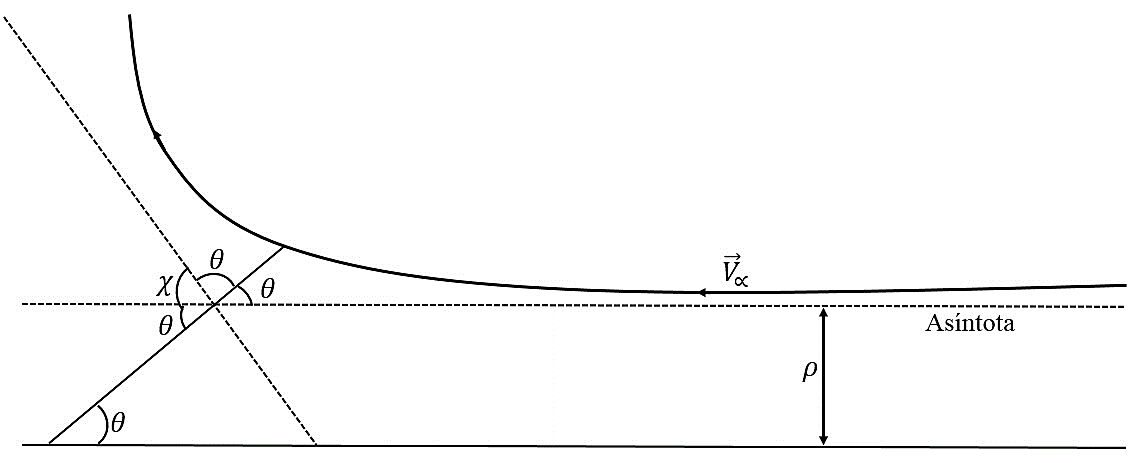
\includegraphics[width=7.01528in,height=2.87639in]{Imagenes/media/image64.png}Considérese
el siguiente esquema, el cual muestra la dirección en que viaja la
partícula:

\includegraphics[width=6.25in,height=2.625in]{Imagenes/media/image65.gif}

\includegraphics[width=6.22917in,height=3.0625in]{Imagenes/media/image66.gif}

Se sabe que la partícula lleva consigo un momento angular, cuya magnitud
viene dada por:

\[l = mrv\]

Para este caso, se tiene que \(m = \mu\), \(r = \rho\) y
\(v = V_{\propto}\), es de tener en cuenta que \(\rho\) corresponde a la
distancia de impacto, de esta manera, la ecuación (160) toma la forma:

\(l = \mu\rho V_{\propto}\)

Por otro lado, la energía es entonces:

\(E = \frac{1}{2}\mu V_{\propto}\)\textsuperscript{2}

Por otro lado, para esta situación se va a utilizar la ecuación de
órbitas deducida en el capítulo 3, para la descripción de este sistema,
como ya se había visto, se sabe que:

\[\theta = \int_{r_{\min}}^{r_{\max}\ }\frac{\frac{l}{r^{2}}dr}{\sqrt{2\mu\left\lbrack E - U(r) \right\rbrack - \frac{l^{2}}{r^{2}}}}\]

De esta manera, llevando (161) y (162) a (163):

\[\theta = \int_{r_{\min}}^{\alpha\ }\frac{\frac{\mu\rho V_{\propto}}{r^{2}}}{\sqrt{2\mu\left( \frac{1}{2}\mu V_{\propto}^{\ 2} \right) - 2\mu\left( \frac{\alpha}{r} \right) - \frac{\mu^{2}\rho^{2}V_{\propto}^{2}}{r^{2}}}}dr\]

\[\theta = \int_{r_{\min}}^{\alpha\ }\frac{\frac{\mu\rho V_{\propto}}{r^{2}}}{\sqrt{\mu^{2}V_{\propto}^{\ 2} - 2\frac{\mu\alpha}{r} - \frac{\mu^{2}\rho^{2}V_{\propto}^{2}}{r^{2}}}}dr\]

\[\theta = \int_{r_{\min}}^{\alpha\ }\frac{\frac{\rho}{r^{2}}}{\sqrt{1 - \frac{2}{\mu V_{\propto}^{\ 2}}\left( \frac{\alpha}{r} \right) - \frac{\rho^{2}}{r^{2}}}}dr\]

Para la solución de la integral (164) se hace el siguiente cambio de
variable:

\[u = \frac{\rho}{r},\ \ \ \ \ \ \ \ \ \ \ \ \ du = - \frac{\rho}{r^{2}}dr\]

De esta forma:

\[\theta = - \int_{r_{\min}}^{\alpha\ }\frac{du}{\sqrt{1 - \frac{2}{\mu V_{\propto}^{\ 2}}\left( \frac{\alpha}{\rho} \right)u - u^{2}}} = - \int_{r_{\min}}^{\alpha\ }\frac{du}{\sqrt{1 - \left( u^{2} + \frac{2}{\mu V_{\propto}^{\ 2}}\left( \frac{\alpha}{\rho} \right)u \right)}}\]

Completando cuadrados:

\[\theta = - \int_{r_{\min}}^{\alpha\ }\frac{du}{\sqrt{1 + \frac{\alpha^{2}}{\mu^{2}V_{\propto}^{\ 4}\rho^{2}} - \left( u^{2} + \frac{2}{\mu V_{\propto}^{\ 2}}\left( \frac{\alpha}{\rho} \right)u + \frac{\alpha^{2}}{\mu^{2}V_{\propto}^{\ 4}\rho^{2}} \right)}}dr\]

Haciendo ahora:

\[A^{2} = 1 + \frac{\alpha^{2}}{\mu^{2}V_{\propto}^{\ 4}\rho^{2}}\]

Entonces:

\[\theta = - \int_{r_{\min}}^{\alpha\ }\frac{du}{\sqrt{A^{2} - \left( u + \frac{\alpha}{\mu V_{\propto}^{\ 2}\rho} \right)^{2}}}dr\]

\[\theta = - \left\lbrack - {arcocos}\left( \frac{u + \frac{\alpha}{\mu V_{\propto}^{\ 2}\rho}}{\sqrt{1 + \frac{\alpha^{2}}{\mu^{2}V_{\propto}^{\ 4}\rho^{2}}}} \right) \right\rbrack\]

\[\theta = {arcocos}\left( \frac{\frac{\alpha}{\mu V_{\propto}^{\ 2}\rho}}{\sqrt{1 + \frac{\alpha^{2}}{\mu^{2}V_{\propto}^{\ 4}\rho^{2}}}} \right)\]

\[\cos\theta = \frac{\frac{\alpha}{\mu V_{\propto}^{\ 2}\rho}}{\sqrt{1 + \frac{\alpha^{2}}{\mu^{2}V_{\propto}^{\ 4}\rho^{2}}}}\]

Como la integral fue resuelta por sustitución trigonométrica, a partir
el triángulo que se puede construir de allí, se da que:

\[\tan\theta = \frac{\frac{1}{1}}{\frac{\alpha}{\mu V_{\propto}^{\ 2}\rho}} \rightarrow \tan\theta = \frac{\mu V_{\propto}^{\ 2}\rho}{\alpha}\]

\[\rho = \frac{\alpha}{\mu V_{\propto}^{\ 2}}\tan\theta\]

Como \(\theta = \frac{\pi - \chi}{2},\) se cumple que:

\[\rho = \frac{\alpha}{\mu V_{\propto}^{\ 2}}\tan\left( \frac{\pi}{2} - \frac{\chi}{2} \right)\]

\[\rho = \frac{\alpha}{\mu V_{\propto}^{\ 2}}\frac{{sen}\left( \frac{\pi}{2} - \chi/2 \right)}{\cos\left( \frac{\pi}{2} - \chi/2 \right)}\]

\(\rho = \frac{\alpha}{\mu V_{\propto}^{\ 2}}\left\lbrack \frac{{sen}\left( \frac{\pi}{2} \right)\cos{\left( \frac{\chi}{2} \right) - {sen}\left( \frac{\chi}{2} \right)\cos\left( \frac{\pi}{2} \right)}}{\cos\left( \frac{\pi}{2} \right)\cos{\left( \frac{\chi}{2} \right) +}{sen}\left( \frac{\pi}{2} \right){sen}\left( \frac{\chi}{2} \right)} \right\rbrack\)

En el S-C, se tiene entonces que:

\[\mathbf{\rho =}\frac{\mathbf{\alpha}}{\mathbf{\mu}\mathbf{V}_{\mathbf{\propto}}^{\mathbf{\ 2}}}\mathbf{\cot}\left( \frac{\mathbf{\chi}}{\mathbf{2}} \right)\mathbf{\ \ \ \ \ \ \ \ \ \ \ \ \ \ }\]

\textbf{EXPERIMENTO DE RUTHERFORD}

En 1911, el físico y químico Ernest Rutherford y sus colaboradores
bombardearon una fina lámina de oro con partículas alfa (positivas),
procedentes de un material radiactivo, a gran velocidad. El experimento
permitió observar el siguiente comportamiento en las partículas
lanzadas:

\begin{itemize}
\item
  La mayor parte de ellas atravesaron la lámina sin cambiar de
  dirección, como era de esperar.
\item
  Algunas se desviaron considerablemente.
\item
  Unas pocas partículas rebotaron hacia la fuente de emisión.
\end{itemize}

El comportamiento de las partículas no podía ser explicado con el modelo
de Thomson, así que Rutherford lo abandonó y sugirió otro basado en el
átomo nuclear.

Modelo de Thomson: De acuerdo con este modelo, en el cual la carga
positiva de cada átomo está distribuida de forma homogénea, las
partículas positivas que atraviesan la lámina no deberían ser
apreciablemente desviadas de su trayectoria inicial. Evidentemente, esto
no ocurría.

Modelo de Rutherford: La carga positiva está concentrada en un núcleo
central, de manera que las partículas positivas que pasan muy cerca de
él se desvían bastante de su trayectoria inicial y sólo aquellas pocas
que chocan directamente con el núcleo regresan en la dirección de la que
proceden.

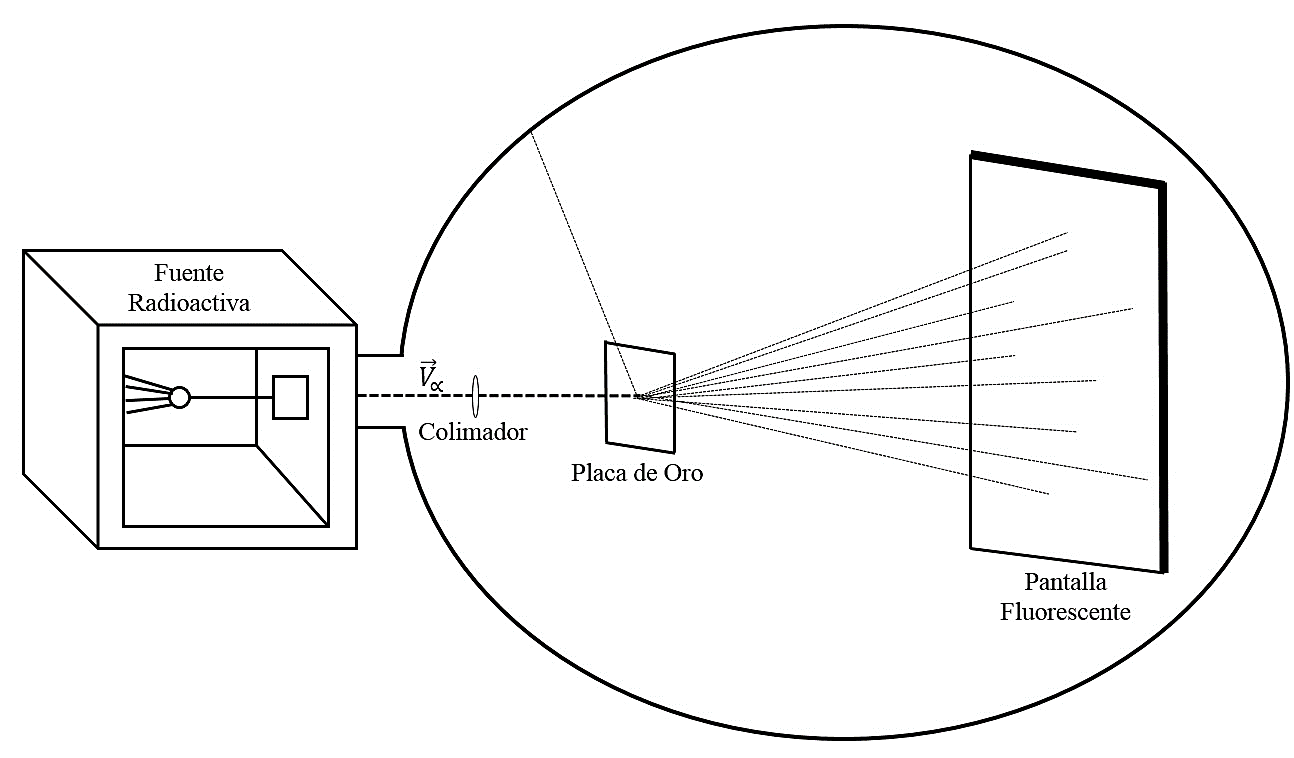
\includegraphics[width=7.13542in,height=4.22917in]{Imagenes/media/image67.png}En
el experimento de Rutherford se procede a estudiar el caso de dispersión
de muchas partículas bajo la acción de una fuerza de tipo central, de la
forma \(\overrightarrow{F} = \frac{\alpha}{r^{2}}\widehat{a_{r}}\) en el
S-C, para esto considérese el esquema mostrado en la \emph{figura 48}:

\includegraphics[width=5.33333in,height=2.09375in]{Imagenes/media/image68.gif}

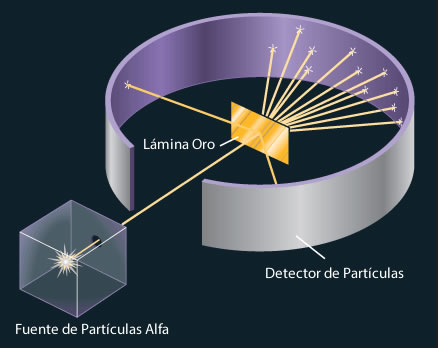
\includegraphics[width=5.25736in,height=4.17708in]{Imagenes/media/image69.jpeg}

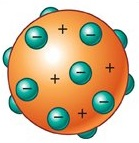
\includegraphics[width=1.95833in,height=2.01469in]{Imagenes/media/image70.jpeg}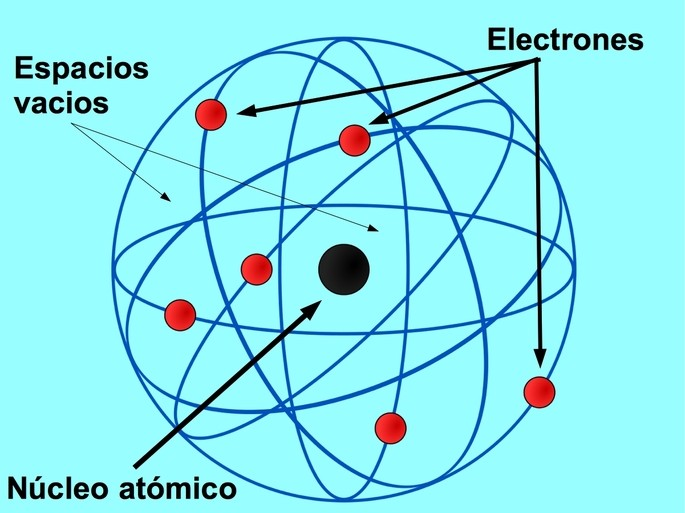
\includegraphics[width=3.57466in,height=2.67708in]{Imagenes/media/image71.jpeg}

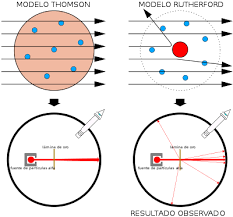
\includegraphics[width=3.43371in,height=3.19792in]{Imagenes/media/image72.png}

Pártase de la siguiente relación de proporcionalidad:

\[N_{d}(dt,\Omega) \propto \frac{N_{i}(dt,\Omega)N_{d}}{s}\]

\(N_{d}\) representa el número de partículas dispersadas y \(N_{i}\) el
número de partículas incidente, la expresión que relaciona el número de
partículas con los de la fuente viene dada por:

\[Id\Omega = - d\sigma JN_{0}\ \ \ \ \ \ \ \ \ \]

Donde \(Id\Omega\) es función del número de partículas y de la fuente,
el signo menos hace parte de la conservación de la masa, \(d\sigma\)
corresponde al diferencial de área del colimador y \(N_{0}\) el número
atómico del elemento del cual estaba hecha la placa, en este caso, el
número atómico del oro, a partir de la ecuación (166) se tiene a los que
se le denomina SECCIÓN EFICAZ:

\[\frac{I}{JN_{0}\ } = \left| \frac{d\sigma}{d\Omega} \right|\]

Como se está trabajando en el S-C, se sabe que \(\theta = \chi\), por lo
tanto:

\[I2\pi{sen}\chi d\chi = - 2\pi\rho d\rho JN_{0}\]

En este caso, se toma \(d\sigma = \rho d\rho\) porque se supone que el
agujero del colimador posee un radio \(\rho\) y desde el agujero al
borde del colimador hay una distancia \(d\rho\), de esta manera:

\[\frac{I}{JN_{0}\ } = \frac{\rho}{{sen}\chi}\left| \frac{d\rho}{d\chi} \right| = \frac{d\sigma}{d\Omega}\]

\[\mathbf{d\sigma =}\frac{\mathbf{\rho}}{\mathbf{sen}\mathbf{\chi}}\left| \frac{\mathbf{d\rho}}{\mathbf{d\chi}} \right|\mathbf{d}\mathbf{\Omega}\mathbf{\ \ \ \ \ \ \ \ \ \ }\]

\[\mathbf{\rho =}\frac{\mathbf{\alpha}}{\mathbf{\mu}\mathbf{V}_{\mathbf{\propto}}^{\mathbf{\ 2}}}\mathbf{\cot}\left( \frac{\mathbf{\chi}}{\mathbf{2}} \right)\mathbf{\ \ \ \ \ \ \ \ \ \ \ \ \ \ }\]

La ecuación (167) corresponde a la sección eficaz obtenida por
Rutherford para su experimento, por otro lado, a partir del resultado
obtenido en (165), se tiene que:

\[\frac{d\rho}{d\chi} = - \frac{1}{2}\frac{\alpha}{\mu V_{\propto}^{\ 2}}\csc^{2}\left( \frac{\chi}{2} \right)\ \ \ \ \ \]

Llevando (168) a (167):

\[d\sigma = \frac{1}{2}\frac{\alpha}{\mu V_{\propto}^{\ 2}}\frac{\cot\left( \frac{\chi}{2} \right)}{{sen}\chi}\left| \frac{\alpha}{\mu V_{\propto}^{\ 2}}\csc^{2}\left( \frac{\chi}{2} \right) \right|d\Omega\]

\[d\sigma = \frac{1}{2}\left( \frac{\alpha}{\mu V_{\propto}^{\ 2}} \right)^{2}\frac{\cos\left( \frac{\chi}{2} \right)}{{sen}\left( \frac{\chi}{2} \right)}\frac{1}{{sen}^{2}\left( \frac{\chi}{2} \right)}\frac{1}{{sen}(\chi)}d\Omega\]

Como \({sen}(\chi) = 2{sen}(\chi/2)\cos(\chi/2),\ \)de esta manera:

\[d\sigma = \frac{1}{2}\left( \frac{\alpha}{\mu V_{\propto}^{\ 2}} \right)^{2}\frac{\cos\left( \frac{\chi}{2} \right)}{{sen}^{3}{\left( \frac{\chi}{2} \right)2{sen}{\left( \frac{\chi}{2} \right)\cos\left( \frac{\chi}{2} \right)}}}d\Omega\]

\[\mathbf{d\sigma =}\left( \frac{\mathbf{\alpha}}{\mathbf{2}\mathbf{\mu}\mathbf{V}_{\mathbf{\propto}}^{\mathbf{\ 2}}} \right)^{\mathbf{2}}\frac{\mathbf{d}\mathbf{\Omega}}{\mathbf{sen}^{\mathbf{4}}\left( \frac{\mathbf{\chi}}{\mathbf{2}} \right)}\mathbf{\ \ \ \ldots\ldots.}\]

\(\mathbf{\ SC\ \ \ \ \ \ \ \ }\)\textbf{ECUACIÓN DE DISPERSIÓN DE
RUTHERFORD}

\includegraphics[width=5.57292in,height=1.09375in]{Imagenes/media/image73.emf}

La expresión (169) corresponde a la ecuación de dispersión de Rutherford
en el S-C.

Ahora, se procede a encontrar la ecuación anterior en un sistema de
laboratorio S-L, las partículas dispersantes de la placa de oro, se
encuentra en reposo, según la teoría de colisiones elásticas el punto
\(B\) se encuentra sobre la circunferencia se encuentra sobre la
circunferencia, en este caso:

\[\overline{OB} = \overline{OC}\]

Como se tiene un triángulo isósceles, entonces:

\[\theta_{2} = \alpha\]

\[\chi + 2\theta_{2} = \pi\]

\[\chi = \pi - 2\theta_{2}\]

De esta manera:

\[d\sigma = 2\pi\rho\left| \frac{d\rho}{d\chi} \right|d\chi\]

\[\mathbf{\rho =}\frac{\mathbf{\alpha}}{\mathbf{\mu}\mathbf{V}_{\mathbf{\propto}}^{\mathbf{\ 2}}}\mathbf{\cot}\left( \frac{\mathbf{\chi}}{\mathbf{2}} \right)\mathbf{\ \ \ \ \ \ \ \ \ \ \ \ \ \ }\]

\[\frac{d\rho}{d\chi} = - \frac{1}{2}\frac{\alpha}{\mu V_{\propto}^{\ 2}}\csc^{2}\left( \frac{\chi}{2} \right)\]

\[d\sigma = 2\pi\left( \frac{\alpha}{\mu V_{\propto}^{\ 2}} \right)^{2}\frac{\cos\left( \frac{\chi}{2} \right)}{{sen}\left( \frac{\chi}{2} \right)}\left( \frac{1}{2} \right)\left( \frac{- 1}{{sen}^{2}\left( \frac{\chi}{2} \right)} \right)d\chi\]

\[d\sigma_{2} = - \pi\left( \frac{\alpha}{\mu V_{\propto}^{\ 2}} \right)^{2}\frac{\cos\left( \frac{\pi}{2} - \theta_{2} \right)}{{sen}^{3}\left( \frac{\pi}{2} - \theta_{2} \right)}\left( - 2d\theta_{2} \right)\]

\[d\sigma_{2} = 2\pi\left( \frac{\alpha}{\mu V_{\propto}^{\ 2}} \right)^{2}\frac{{\lbrack cos}\left( \frac{\pi}{2} \right)\cos{\left( \theta_{2} \right) + {sen}{\left( \frac{\pi}{2} \right){sen}\left( \theta_{2} \right)}}\rbrack}{{\lbrack sen}{\left( \frac{\pi}{2} \right)\cos\left( \theta_{2} \right)} - {sen}\left( \theta_{2} \right)\cos{\left( \frac{\pi}{2} \right)\rbrack}}\ d\theta_{2}\]

\[d\sigma_{2} = 2\pi\left( \frac{\alpha}{\mu V_{\propto}^{\ 2}} \right)^{2}\frac{{sen}\theta_{2}d\theta_{2}}{\mathbf{\cos}^{\mathbf{3}}\mathbf{\theta}_{\mathbf{2}}}\]

Por lo tanto:

\[\mathbf{d}\mathbf{\sigma}_{\mathbf{2}}\mathbf{=}\left( \frac{\mathbf{\alpha}}{\mathbf{\mu}\mathbf{V}_{\mathbf{\propto}}^{\mathbf{\ 2}}} \right)^{\mathbf{2}}\frac{\mathbf{d}\mathbf{\Omega}_{\mathbf{2}}}{\mathbf{\cos}^{\mathbf{3}}\mathbf{\theta}_{\mathbf{2}}}\mathbf{\ \ \ \ \ \ \ \ \ \ \ }\]

\textbf{Sección eficaz de Rutherford para el SL}

La expresión (170) corresponde a la ecuación de dispersión de Rutherford
en el S-L.

Analícense ahora dos casos relacionados con el tamaño de las masas:

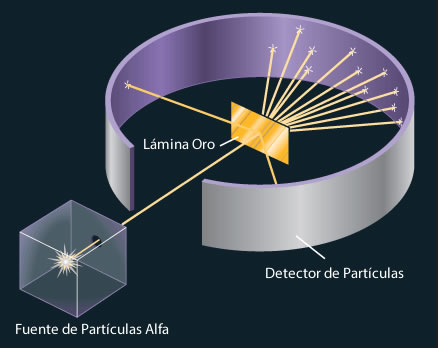
\includegraphics[width=5.25736in,height=4.17708in]{Imagenes/media/image69.jpeg}

\includegraphics[width=4.83122in,height=2.73958in]{Imagenes/media/image74.gif}

\includegraphics[width=5.33333in,height=2.09375in]{Imagenes/media/image68.gif}

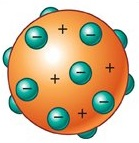
\includegraphics[width=1.95833in,height=2.01469in]{Imagenes/media/image70.jpeg}
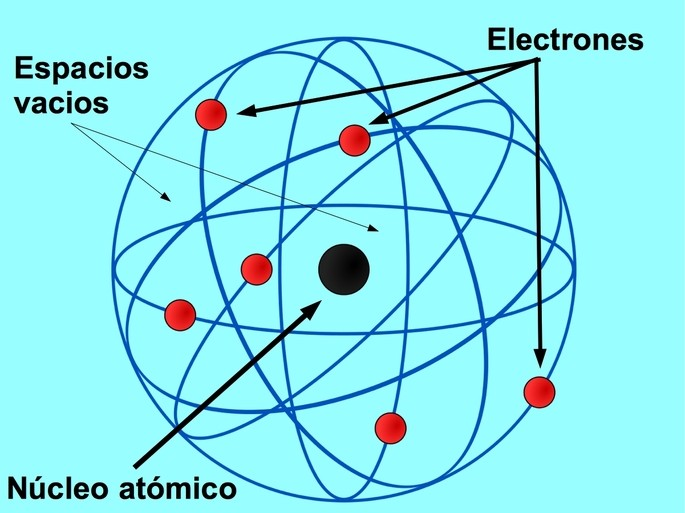
\includegraphics[width=3.57466in,height=2.67708in]{Imagenes/media/image71.jpeg}

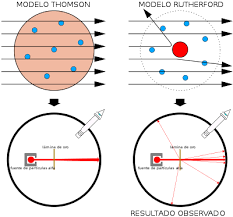
\includegraphics[width=3.43371in,height=3.19792in]{Imagenes/media/image72.png}

\includegraphics[width=5.57292in,height=1.09375in]{Imagenes/media/image73.emf}

1.67262 × 10\textsuperscript{-24}~g masa del protón \textbf{1840} mayor
que la masa del electrón

el núcleo ocupa solamente 1/1013 del volumen total del átomo

1 pm = 1 × 10\textsuperscript{-12}~m radio del átomo 100 pm

radio del núcleo atómico es solamente de 0.005 pm

\uline{CASO I}: Si las partículas dispersantes son muy grandes con
respecto a las partículas dispersadas \(m_{2} \gg m_{1}\):

\[\tan{\theta_{1} = \frac{m_{2}{sen}\chi}{m_{1} + m_{2}\cos\chi}}\]

\[\mu = \frac{m_{1}m_{2}}{m_{1} + m_{2}}\]

Para este caso \(\mu \approx m_{1}\) además:

\[\tan\theta_{1} \approx \tan\chi \rightarrow \theta_{1} = \chi\]

Por lo tanto:

\[\mathbf{d\sigma =}\left( \frac{\mathbf{\alpha}}{\mathbf{2}\mathbf{\mu}\mathbf{V}_{\mathbf{\propto}}^{\mathbf{\ 2}}} \right)^{\mathbf{2}}\frac{\mathbf{d}\mathbf{\Omega}}{\mathbf{sen}^{\mathbf{4}}\left( \frac{\mathbf{\chi}}{\mathbf{2}} \right)}\mathbf{\ \ \ \ \ \ \ \ \ \ \ \ \ }\]

\[\mathbf{d}\mathbf{\sigma}_{\mathbf{1}}\mathbf{=}\left( \frac{\mathbf{\alpha}}{\mathbf{2}\mathbf{m}_{\mathbf{1}}\mathbf{V}_{\mathbf{\propto}}^{\mathbf{\ 2}}} \right)^{\mathbf{2}}\frac{\mathbf{d}\mathbf{\Omega}_{\mathbf{1}}}{\mathbf{sen}^{\mathbf{4}}\left( \frac{\mathbf{\theta}_{\mathbf{1}}}{\mathbf{2}} \right)}\mathbf{\ \ \ \ \ \ \ \ \ \ \ }\]

Si se introduce la energía de la forma:

\[\mathbf{E}_{\mathbf{1}} = \frac{1}{2}m_{1}V_{\propto}^{\ 2} + \left( \frac{\alpha}{r} \right) \rightarrow 2\mathbf{E}_{\mathbf{1}} = m_{1}V_{\propto}^{\ 2}\]

La ecuación (171) toma la forma:

\[\mathbf{d}\mathbf{\sigma}_{\mathbf{1}}\mathbf{=}\left( \frac{\mathbf{\alpha}}{\mathbf{4}\mathbf{E}_{\mathbf{1}}} \right)^{\mathbf{2}}\frac{\mathbf{d}\mathbf{\Omega}_{\mathbf{1}}}{\mathbf{sen}^{\mathbf{4}}\left( \frac{\mathbf{\theta}_{\mathbf{1}}}{\mathbf{2}} \right)}\mathbf{\ \ \ \ \ \ \ \ \ \ \ \ \ \ \ }\]

\uline{CASO II}: Si las masas de las partículas dispersantes son igual a
las masas de las partículas dispersadas, cabe destacar que después de la
colisión, no es posible conocer cuáles son las partículas dispersadas y
cuáles son las partículas dispersantes. Para este caso, se parte de la
forma que toma la masa reducida cuando \(m_{1} = m_{2}\), estos es:

\[\mu = \frac{m_{1}m_{2}}{m_{1} + m_{2}} \approx \frac{m_{1}^{\ 2}}{2m_{1}} \approx \frac{1}{2}m_{1}\]

Asimismo:

\[\tan\theta_{1} = \frac{m_{2}{sen}\chi}{m_{1} + m_{2}\cos\chi} \approx \frac{m_{2}{sen}\chi}{m_{2}\left( 1 + \cos\chi \right)} \approx \frac{{sen}\chi}{1 + \cos\chi}\]

\[\tan\theta_{1} = \frac{2{sen}{\left( \frac{\chi}{2} \right)\cos\left( \frac{\chi}{2} \right)}}{2\cos^{2}\left( \frac{\chi}{2} \right)} = \tan\left( \frac{\chi}{2} \right)\]

Esto indica que \(\theta_{1} = \frac{\chi}{2}\), entonces
\(d\chi = 2d\theta_{1}\), de esta manera:

\[d\sigma = 2\pi\rho\left| \frac{d\rho}{d\chi} \right|d\chi\]

\[\mathbf{\rho =}\frac{\mathbf{\alpha}}{\mathbf{\mu}\mathbf{V}_{\mathbf{\propto}}^{\mathbf{\ 2}}}\mathbf{\cot}\left( \frac{\mathbf{\chi}}{\mathbf{2}} \right)\mathbf{\ \ \ \ \ \ \ \ \ \ \ \ \ \ }\]

\[\frac{d\rho}{d\chi} = - \frac{1}{2}\frac{\alpha}{\mu V_{\propto}^{\ 2}}\csc^{2}\left( \frac{\chi}{2} \right)\]

\[d\sigma = 2\pi\left( \frac{\alpha}{\mu V_{\propto}^{\ 2}} \right)^{2}\frac{\cos\left( \frac{\chi}{2} \right)}{{sen}\left( \frac{\chi}{2} \right)}\left( \frac{1}{2} \right)\left( \frac{- 1}{{sen}^{2}\left( \frac{\chi}{2} \right)} \right)d\chi\]

\[d\sigma_{1} = {2\pi\left( \frac{\alpha}{\mu V_{\propto}^{\ 2}} \right)}^{2}\frac{\cos\theta_{1}}{{sen}^{3}\theta_{1}}\frac{{sen}\theta_{1}}{{sen}\theta_{1}}d\theta_{1}\]

\[d\sigma_{1} = \left( \frac{\alpha}{\mu V_{\propto}^{\ 2}} \right)^{2}\frac{\cos\theta_{1}}{{sen}^{4}\theta_{1}}2\pi{sen}{\theta_{1}d\theta_{1}}\]

\[\mathbf{d}\mathbf{\sigma}_{\mathbf{1}}\mathbf{=}\left( \frac{\mathbf{\alpha}}{\mathbf{E}_{\mathbf{1}}} \right)^{\mathbf{2}}\frac{\mathbf{\cos}\mathbf{\theta}_{\mathbf{1}}}{\mathbf{sen}^{\mathbf{4}}\mathbf{\theta}_{\mathbf{1}}}\mathbf{d}\mathbf{\Omega}_{\mathbf{1}}\mathbf{\ \ \ \ \ \ \ \ \ \ \ }\]

\[\mathbf{d}\mathbf{\sigma}_{\mathbf{2}}\mathbf{=}\left( \frac{\mathbf{\alpha}}{\mathbf{\mu}\mathbf{V}_{\mathbf{\propto}}^{\mathbf{\ 2}}} \right)^{\mathbf{2}}\frac{\mathbf{d}\mathbf{\Omega}_{\mathbf{2}}}{\mathbf{\cos}^{\mathbf{3}}\mathbf{\theta}_{\mathbf{2}}}\mathbf{\ \ \ \ \ \ \ \ \ \ \ }\]

\[\mathbf{d}\mathbf{\sigma}_{\mathbf{2}}\mathbf{=}\left( \frac{\mathbf{\alpha}}{\frac{\mathbf{1}}{\mathbf{2}}{\mathbf{m}_{\mathbf{1}}\mathbf{V}}_{\mathbf{\propto}}^{\mathbf{\ 2}}} \right)^{\mathbf{2}}\frac{\mathbf{\cos}\mathbf{\theta}_{\mathbf{2}}\mathbf{d}\mathbf{\Omega}_{\mathbf{2}}}{\mathbf{\cos}^{\mathbf{4}}\mathbf{\theta}_{\mathbf{2}}}\mathbf{\ \ \ \ \ \ \ \ \ \ \ }\]

\[\mathbf{d}\mathbf{\sigma}_{\mathbf{2}}\mathbf{=}\left( \frac{\mathbf{\alpha}}{\mathbf{E}_{\mathbf{1}}} \right)^{\mathbf{2}}\frac{\mathbf{\cos}\mathbf{\theta}_{\mathbf{2}}\mathbf{d}\mathbf{\Omega}_{\mathbf{2}}}{\mathbf{\cos}^{\mathbf{4}}\mathbf{\theta}_{\mathbf{2}}}\]

\[\mathbf{d\sigma = d}\mathbf{\sigma}_{\mathbf{1}}\mathbf{+ d}\mathbf{\sigma}_{\mathbf{2}}\mathbf{=}\left( \frac{\mathbf{\alpha}}{\mathbf{E}_{\mathbf{1}}} \right)^{\mathbf{2}}\frac{\mathbf{\cos}\mathbf{\theta}_{\mathbf{1}}}{\mathbf{sen}^{\mathbf{4}}\mathbf{\theta}_{\mathbf{1}}}\mathbf{d}\mathbf{\Omega}_{\mathbf{1}}\mathbf{\ \  +}\left( \frac{\mathbf{\alpha}}{\mathbf{E}_{\mathbf{1}}} \right)^{\mathbf{2}}\frac{\mathbf{\cos}\mathbf{\theta}_{\mathbf{2}}\mathbf{d}\mathbf{\Omega}_{\mathbf{2}}}{\mathbf{\cos}^{\mathbf{4}}\mathbf{\theta}_{\mathbf{2}}}\mathbf{\ \ \ \ \ \ \ \ \ \ \ }\]

\[\mathbf{d\sigma = d}\mathbf{\sigma}_{\mathbf{1}}\mathbf{+ d}\mathbf{\sigma}_{\mathbf{2}}\mathbf{=}\left( \frac{\mathbf{\alpha}}{\mathbf{E}_{\mathbf{1}}} \right)^{\mathbf{2}}\left( \frac{\mathbf{1}}{\mathbf{sen}^{\mathbf{4}}\mathbf{\theta}_{\mathbf{1}}}\mathbf{\ \  +}\frac{\mathbf{1}}{\mathbf{\cos}^{\mathbf{4}}\mathbf{\theta}_{\mathbf{2}}}\mathbf{\ } \right)\mathbf{cos\theta d}\mathbf{\Omega}\mathbf{\ \ \ \ \ \ \ \ \ \ }\]

Finalmente, se va a encontrar la ley de dispersión coulombiana o de
Rutherford para las partículas radioactivas \(\alpha\) en función de la
pérdida de energía en la colisión elástica, para esto se parte de la
magnitud de la velocidad dada por:

\[\left| {\overrightarrow{V}}_{2}' \right| = \frac{2m_{1}{sen}\left( \frac{\chi}{2} \right)}{m_{1} + m_{2}}\left| {\overrightarrow{V}}_{\propto} \right|\]

Al llevar esta velocidad a la energía, se tiene que:

\[E = \frac{1}{2}m_{2}\left| '{{\overrightarrow{V}}_{2}}^{2} \right|\]

\[E = \frac{2\mu^{2}}{m_{2}}{sen}^{2}\left( \frac{\chi}{2} \right)\left| {\overrightarrow{V}}_{\propto} \right|^{2}\]

Por lo tanto:

\[d\sigma = 2\pi\rho\left| \frac{d\rho}{d\chi} \right|d\chi\]

\[\mathbf{\rho =}\frac{\mathbf{\alpha}}{\mathbf{\mu}\mathbf{V}_{\mathbf{\propto}}^{\mathbf{\ 2}}}\mathbf{\cot}\left( \frac{\mathbf{\chi}}{\mathbf{2}} \right)\mathbf{\ \ \ \ \ \ \ \ \ \ \ \ \ \ }\]

\[\frac{d\rho}{d\chi} = - \frac{1}{2}\frac{\alpha}{\mu V_{\propto}^{\ 2}}\csc^{2}\left( \frac{\chi}{2} \right)\]

\[d\sigma = 2\pi\left( \frac{\alpha}{\mu V_{\propto}^{\ 2}} \right)^{2}\frac{\cos\left( \frac{\chi}{2} \right)}{{sen}\left( \frac{\chi}{2} \right)}\left( \frac{1}{2} \right)\left( \frac{1}{{sen}^{2}\left( \frac{\chi}{2} \right)} \right)d\chi\]

De (174):

\[E = \frac{2\mu^{2}}{m_{2}}{sen}^{2}\left( \frac{\chi}{2} \right)\left| {\overrightarrow{V}}_{\propto} \right|^{2}\]

\[{sen}{\left( \frac{\chi}{2} \right) = \sqrt{\frac{m_{2}E}{2\mu^{2}V_{\propto}^{\ 2}}}}\]

Derivando (176) con respecto a la energía:

\[\frac{1}{2}\left\lbrack \cos\left( \frac{\chi}{2} \right) \right\rbrack d\chi = \frac{1}{2\sqrt{\frac{m_{2}E}{2\mu^{2}V_{\propto}^{\ 2}}}}\frac{m_{2}}{2\mu^{2}V_{\propto}^{\ 2}}dE\]

Llevando (177) a (175) se da que:

\[d\sigma = 2\pi\left( \frac{\alpha}{\mu V_{\propto}^{\ 2}} \right)^{2}\frac{\cos\left( \frac{\chi}{2} \right)}{{sen}\left( \frac{\chi}{2} \right)}\left( \frac{1}{2} \right)\left( \frac{1}{{sen}^{2}\left( \frac{\chi}{2} \right)} \right)d\chi\]

\[d\sigma = 2\pi\left( \frac{\alpha}{\mu V_{\propto}^{\ 2}} \right)^{2}\left( \frac{m_{2}}{(2)2\mu^{2}V_{\propto}^{\ 2}}\frac{dE}{\sqrt{\frac{m_{2}E}{2\mu^{2}V_{\propto}^{\ 2}}}} \right)\frac{1}{\frac{m_{2}E}{2\mu^{2}V_{\propto}^{\ 2}}\sqrt{\frac{m_{2}E}{2\mu^{2}V_{\propto}^{\ 2}}}}\]

\[d\sigma = 2\pi\frac{\alpha^{2}}{\mu^{2}V_{\propto}^{\ 4}}\left( \frac{m_{2}}{(2)2\mu^{2}V_{\propto}^{\ 2}}\frac{dE}{\frac{m_{2}E}{2\mu^{2}V_{\propto}^{\ 2}}} \right)\frac{1}{\frac{m_{2}E}{2\mu^{2}V_{\propto}^{\ 2}}}\]

\[\mathbf{d\sigma =}\left( \frac{\mathbf{2}\mathbf{\pi}\mathbf{\alpha}^{\mathbf{2}}}{\mathbf{m}_{\mathbf{2}}\mathbf{V}_{\mathbf{\propto}}^{\mathbf{\ 2}}} \right)\frac{\mathbf{dE}}{\mathbf{E}^{\mathbf{2}}}\mathbf{\ \ \ \ \ \ \ \ \ \ \ }\]

La ecuación (178) representa la distribución de las partículas
dispersadas con respecto a la energía transferida en la colisión
elástica.

\textbf{Capítulo 5 Dinámica de Hamilton}

La dinámica de Hamilton fue formulada en 1833 por el matemático, físico
y astrónomo irlandés William Rowan Hamilton. La dinámica de Hamilton es
una reformulación de la mecánica clásica, así como la dinámica de
Lagrange. Una de las variedades principalmente usadas en la mecánica
clásica y fundamentalmente en la dinámica Hamiltoniana son los espacios
simplécticos, sin referir a cualquiera de los conceptos de fuerza de la
dinámica de Lagrange.

La dinámica de Hamilton proporciona grandes ventajas pues las ecuaciones
de Hamilton son de primer orden lo que implica que la solución de estas
sea más sencilla de obtener, a diferencia de las ecuaciones de Lagrange
que son de segundo orden. En el enfoque Hamiltoniano existe un nuevo
conjunto de términos que son denominados momentos conjugados o momentos
canónicos, esto es lo más costoso de trabajar con este enfoque, ya que
se busca expresar las velocidades en términos de estos momentos
conjugados para construir el Hamiltoniano.

La solución de problemas, usando la dinámica de Hamilton puede que
algunas veces resulte más tediosa la obtención de la solución que con el
enfoque de Lagrange, pues, al final de cuentas el resultado que se
obtiene es el mismo resultado que en la dinámica de Lagrange o con las
Leyes de Newton de movimiento. No obstante, existen otro tipo de
ventajas:

\begin{itemize}
\item
  Las ecuaciones de Hamilton pueden dejarse invariantes con un conjunto
  de transformaciones denominado transformaciones canónicas que son una
  especie de cambio de coordenadas mucho más extensa que la que existe
  en la dinámica de Lagrange.
\item
  La base para la obtención de los resultados más profundos en la teoría
  de la mecánica clásica es proporcionada por el enfoque Hamiltoniano,
  pues este enfoque permite introducir el formalismo del espacio de
  fases, el cual se define como una estructura o variedades simpléctica
  sobre el fibrado cotangente del espacio de configuración.
\end{itemize}

La dinámica de Hamilton, puede considerarse como un enfoque equivalente
a la dinámica de Lagrange, donde la ecuaciones de movimiento vienen
dadas por un sistema de ecuaciones diferenciales de primer orden
ordinarias las cuales se escriben en términos de una nueva función \(H\)
llamada Hamiltoniano del sistema, que en algunos caso puede
interpretarse como la energía total del sistema.

\textbf{PROPIEDADES DE SIMETRÍA}

Tanto la estructura algebráica de grupo como las denominadas Algebras de
Lie, tiene la

peculiaridad de ser las estructuras matemáticas que describen el
concepto clásico de simetría. La Teoría de la Relatividad Restringida
es, en último término, una teoría de las simetrías del espacio vacío y
también del tiempo, descritas por el grupo de Poincaré, grupo de
transformaciones ortogonales, del cual es subgrupo el grupo de Lorentz.

Incluso, la definición del concepto de partícula, en el contexto de la
Teoría Cuántica de los Campos, tal como la formuló Eugene Wigner
(1902-1995), está relacionada con la simetría: "Una partícula es una
representación irreducible del grupo de Poincaré". Tanto la masa de una
partícula como su espín, por ejemplo, se relacionan con formas distintas
de representaciones irreducibles del grupo de Poincaré.~

Pero la simetría, en todas sus formas, tiene una relación directa con la
constancia de ciertas magnitudes fundamentales, con la conservación. Fue
en 1915 cuando la gran matemática Emmy Noether (1982-1935) pudo probar
que toda ley de simetría, tanto en la Mecánica Clásica como en la
Mecánica Cuántica, origina una propiedad de conservación.

La simetría es una propiedad universal tanto en la vida corriente, desde
un punto de vista matemático como desde el quehacer de la Física
Teórica. En realidad, lo que observamos en la vida corriente es siempre
lo repetitivo, lo simétrico, lo que se puede relacionar entre sí por
tener algo común.

En un sentido dinámico, la simetría podemos entenderla como lo que se
repite, lo reiterativo, lo que tiende a ser igual. Es decir, los objetos
que, por mantener la misma geometría, son representativos de otros
objetos. En el Caos matemático encontramos esta concepción de la
simetría en el mundo los fractales.

En la simetría axial tridimensional, el cambio es una rotación con
respecto a un eje, y en el caso de la simetría central, el cambio al que
va asociada es la rotación alrededor de un centro. La simetría axial y
la simetría central son las formas clásicas de simetría de los objetos
del espacio ordinario, sin embargo, cuando hablamos de entidades más
abstractas en la física de las partículas es preciso generalizar el
concepto clásico de simetría.~

La Física clásica de Galileo y Newton, esto es, la mecánica desarrollada
luego por Lagrange, Hamilton, Mapertuis, etc, como la teoría especial de
la relatividad formulada por Einstein, descansan, para poder
desarrollarse, en la postulación implícita de simetría en el contexto
del espacio-tiempo.

Esta postulación de simetría para la formulación y desarrollo de las
leyes de la física constituye tanto lo que entendemos por homogeneidad e
isotropía del espacio, por una parte, como por lo que llamamos
uniformidad del transcurrir del tiempo, por otra.

Considérese el sistema de \(n -\)partículas mostrado en la \emph{figura
49}:

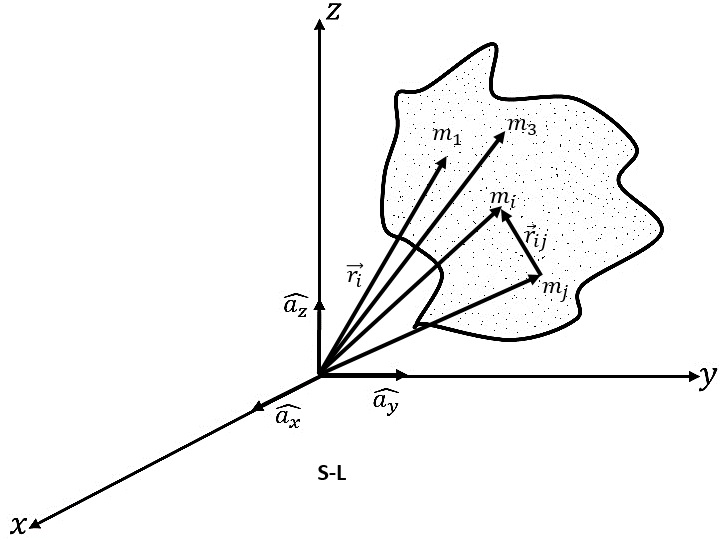
\includegraphics[width=5.94792in,height=4.43017in]{Imagenes/media/image43.jpeg}

Para este sistema se escribe la energía cinética para este sistema de la
forma:

\[T = \frac{1}{2}\sum_{\alpha = 1}^{n}m_{a}\sum_{i = 1}^{3}{\dot{x}}_{ai}^{\ \ \ \ 2}\ \ \ \ \ \ \ \ \ \ \]

La expresión (179) tiene una limitación y es que las coordenadas
cartesianas \({\dot{x}}_{ai}^{\ \ \ \ }\) no son coordenadas
independientes, por esta razón para la energía cinética \(T\) del
sistema de \(n -\)partículas en función de las coordenadas y velocidades
generalizadas, esto es:

\[x_{\alpha i} = x_{\alpha i}\left( q_{1},\ q_{2},q_{3},\ldots,q_{s};t \right)\]

\[{\dot{x}}_{\alpha i} = \sum_{j = 1}^{s}\frac{\partial x_{\alpha i}}{\partial q_{j}}{\dot{q}}_{j} + \frac{\partial x_{\alpha i}}{\partial t}\]

\[{\dot{x}}_{\alpha i} = \frac{\partial x_{\alpha i}}{\partial q_{1}}\dot{q_{1}} + \frac{\partial x_{\alpha i}}{\partial q_{2}}\dot{q_{2}} + \frac{\partial x_{\alpha i}}{\partial q_{3}}\dot{q_{3}} + \ldots + \frac{\partial x_{\alpha i}}{\partial t}\]

De esta manera, la velocidad generalizada está dada por:

\[{\dot{x}}_{\alpha i}^{\ \ \ \ 2} = \left( \sum_{j = 1}^{s}\frac{\partial x_{\alpha i}}{\partial q_{j}}{\dot{q}}_{j} + \frac{\partial x_{\alpha i}}{\partial t} \right)^{2}\]

\[{\dot{x}}_{\alpha i}^{\ \ \ \ 2} = \sum_{j,k}^{}\frac{\partial x_{\alpha i}}{\partial q_{j}}\frac{\partial x_{\alpha i}}{\partial q_{k}}\dot{q_{j}}\dot{q_{k}} + 2\sum_{j,}^{}\frac{\partial x_{\alpha i}}{\partial q_{j}}\frac{\partial x_{\alpha i}}{\partial t}\dot{q_{j}} + \left( \frac{\partial x_{qi}}{\partial t} \right)^{2}\]

De este modo:

\[T = \sum_{\alpha = 1}^{n}{\sum_{i,j,k}^{}{\frac{1}{2}m_{\alpha}}}\frac{\partial x_{\alpha i}}{\partial q_{i}}\frac{\partial x_{\alpha i}}{\partial q_{k}}\dot{q_{j}}\dot{q_{k}} + \sum_{\alpha = 1}^{n}{m_{\alpha}\sum_{i,j}^{}{\frac{\partial x_{\alpha i}}{\partial q_{i}}\frac{\partial x_{\alpha i}}{\partial t}\dot{q_{j}} +}}\sum_{\alpha = 1}^{n}{\frac{1}{2}m_{\alpha}}\sum_{i}^{}\left( \frac{\partial x_{qi}}{\partial t} \right)^{2}\]

Haciendo:

\[a_{jk} = \sum_{\alpha = 1}^{n}{\sum_{i,}^{}{\frac{1}{2}m_{\alpha}}}\frac{\partial x_{\alpha i}}{\partial q_{i}}\frac{\partial x_{\alpha i}}{\partial q_{k}}\]

\[b_{j} = \sum_{\alpha = 1}^{n}{\sum_{i,}^{}{m_{\alpha}\frac{\partial x_{\alpha i}}{\partial q_{i}}\frac{\partial x_{\alpha i}}{\partial t}}}\]

\[c = {\sum_{\alpha = 1}^{n}{\sum_{i}^{}{{\frac{1}{2}m}_{\alpha}\left( \frac{\partial x_{\alpha i}}{\partial t} \right)}}}^{2}\]

Entonces:

\[\mathbf{T =}\sum_{\mathbf{j,k}}^{}{\mathbf{a}_{\mathbf{j,k}}{\dot{\mathbf{q}}}_{\mathbf{j}}}{\dot{\mathbf{q}}}_{\mathbf{k}}\mathbf{+}\sum_{\mathbf{j}}^{}\mathbf{b}_{\mathbf{i}}{\dot{\mathbf{q}}}_{\mathbf{j}}\mathbf{+ c\ \ \ \ \ \ \ }\]

\uline{Simetría I: Homogeneidad del Tiempo}

La homogeneidad del tiempo~intenta explicar que el transcurrir de los
acontecimientos no modifica las leyes de la Física, esto es, que las
leyes de la física en un instante dado son las mismas que en cualquier
instante anterior y seguirán siendo las mismas en los instantes
posteriores.

El sistema de \(n -\)partículas es un sistema cerrado, por lo tanto,
cualquier tipo de observable es independiente del tiempo, por lo tanto
los coeficientes \(b_{j}\) y \(c\) son cero, de esta forma:

\[T = \sum_{j,k}^{}{a_{j,k}{\dot{q}}_{j}}{\dot{q}}_{k}\ \ \ \ \ \ \ \]

A partir de (181) se da que:

\[\frac{\partial T}{\partial{\dot{q}}_{l}} = \sum_{j}^{}{a_{j}{\dot{q}}_{j}} + \sum_{k}^{}a_{k}{\dot{q}}_{k}\]

\[\sum_{l}^{}\frac{\partial T}{\partial{\dot{q}}_{l}}{\dot{q}}_{l} = \sum_{j,l}^{}{a_{j,l}{\dot{q}}_{j}}{\dot{q}}_{l} + \sum_{j,l}^{}{a_{k,l}{\dot{q}}_{k}}{\dot{q}}_{l}\]

Como los subíndices son mudos:

\[\sum_{j}^{}\frac{\partial T}{\partial{\dot{q}}_{j}}{\dot{q}}_{j} = 2\sum_{j,k}^{}{a_{j,k}{\dot{q}}_{j}}{\dot{q}}_{k} = 2T\]

\[\sum_{j}^{}{\frac{\partial T}{\partial{\dot{q}}_{j}}{\dot{q}}_{j} = 2T}\]

Escribiendo el Lagrangiano:

\[L = L\left( q_{j},{\dot{q}}_{j};t \right)\]

\[\frac{dL}{dt} = \sum_{j}^{}{\frac{\partial L}{\partial q_{j}}{\dot{q}}_{j}} + \sum_{j}^{}{\frac{\partial L}{\partial{\dot{q}}_{j}}{\ddot{q}}_{j}} + \frac{\partial L}{\partial t}\]

Para sistemas cerrados o sistemas termodinámicos, el último término se
hace cero, así:

\[\frac{dL}{dt} = \sum_{j}^{}{\frac{d}{dt}\left( \frac{\partial L}{\partial{\dot{q}}_{j}} \right){\dot{q}}_{j}} + \sum_{j}^{}{\frac{\partial L}{\partial{\dot{q}}_{j}}{\ddot{q}}_{j}}\]

\[\sum_{j}^{}{\frac{d}{dt}\left\lbrack \left( \frac{\partial L}{\partial{\dot{q}}_{j}} \right){\dot{q}}_{j} \right\rbrack} = \sum_{j}^{}{\frac{d}{dt}\left( \frac{\partial L}{\partial{\dot{q}}_{j}} \right){\dot{q}}_{j}} + \sum_{j}^{}{\frac{\partial L}{\partial{\dot{q}}_{j}}{\ddot{q}}_{j}}\]

\[\frac{dL}{dt} = \sum_{j}^{}{\frac{d}{dt}\left\lbrack \left( \frac{\partial L}{\partial{\dot{q}}_{j}} \right){\dot{q}}_{j} \right\rbrack}\]

De esta manera:

\[\frac{d}{dt}\left( \sum_{j}^{}{\frac{\partial L}{\partial{\dot{q}}_{j}}{\dot{q}}_{j} - L} \right) = 0\ \ \ \ \ \ \]

La expresión (182) es consecuencia de un teorema de conservación, para
que esta igualdad se cumpla, debe darse que lo que se encuentra dentro
de los paréntesis sea una constante, por conveniencia se va a denotar
por \(H\), así:

\[\sum_{j}^{}{\frac{\partial L}{\partial{\dot{q}}_{j}}{\dot{q}}_{j} - L} = H\]

\[\sum_{j}^{}{\frac{\partial}{\partial{\dot{q}}_{j}}(T - U){\dot{q}}_{j} - L} = H\]

\[\sum_{j}^{}{\frac{\partial T}{\partial{\dot{q}}_{j}}{\dot{q}}_{j} - \sum_{j}^{}{\frac{\partial U}{\partial{\dot{q}}_{j}}{\dot{q}}_{j} -}L} = H\]

\[\sum_{j}^{}{\frac{\partial T}{\partial{\dot{q}}_{j}}{\dot{q}}_{j} - L} = H\ \ \ \ \ \ \ \ \]

Trayendo (182) a (184) y recordando que \(L = T - U\) entonces:

\[2T - (T - U) = H\]

\[T + U = H\ \ \ \ \ \ \ \ \]

La expresión (185) corresponde al teorema de conservación de la energía
total en los sistemas mecánicos holónomos esclerónomos, aquellos
sistemas sometidos a condiciones de ligadura independientes del tiempo
expresables mediante relaciones matemáticas entre sus coordenadas, no
sometidos a fuerzas de disipación, resulta ser una consecuencia
inmediata de la homogeneidad del tiempo, es decir, del hecho de que las
magnitudes fundamentales no dependen explícitamente del transcurrir del
tiempo.

En general, hay una nueva función que es denominada HAMILTONIANO del
sistema \((H)\). En los sistemas mecánicos holónomos esclerónomos, el
Hamiltoniano~\(H\)~se conserva, y como la energía total coincide con el
Hamiltoniano, si no existen fuerzas disipativas, se puede concluir que
la energía total se conserva, es decir:

\[H = cte\]

\textbf{ECUACIONES DE MOVIMIENTO DE HAMILTON}

En primer lugar se toma el Hamiltoniano escrito como:

\[\sum_{j}^{}{\frac{\partial T}{\partial{\dot{q}}_{j}}{\dot{q}}_{j} - L}\left( q_{j},{\dot{q}}_{j};t \right) = H\ \ \ \ \ \ \ \ \ \]

A continuación se introduce lo que corresponde una trasformación de
derivadas, denominada TRANSFORMACIÓN LINEAL DE LEGENDRE. Se dice que dos
funciones diferenciables \(f\) y \(g\ \)son una transformada de Legendre
si cada una de sus primera derivadas son funciones inversas de la otra.
Bajo este concepto, tómese la ecuación de movimiento de Lagrange:

\[\frac{d}{dt}\left( \frac{\partial L}{\partial{\dot{q}}_{j}} \right) - \frac{\partial L}{\partial q_{j}} = 0\]

A partir de la transformación lineal de Legendre, se tiene que:

\[\frac{\partial L}{\partial{\dot{q}}_{j}} = p_{j}\]

Por lo que (186) se puede escribir como:

\[H\left( q_{j},p_{j};t \right) = \sum_{j}^{}{{\dot{q}}_{j}p_{j} - L\left( q_{j},{\dot{q}}_{j};t \right)}\]

De esta forma:

\[dH\left( q_{j},P_{j};t \right) = \sum_{j}^{}{\frac{\partial H}{\partial q_{j}}dq_{j} +}\sum_{j}^{}{\frac{\partial H}{\partial p_{j}}dp_{j} +}\frac{\partial H}{\partial t}dt\ \ \ \ \ \ \ \ \ \]

\[dH\left( q_{j},P_{j};t \right) = \sum_{j}^{}{{\dot{q}}_{j}dp_{j} +}\sum_{j}^{}{p_{j}d{\dot{q}}_{j}} - \sum_{j}^{}\frac{\partial L}{\partial q_{j}}dq_{j} - \sum_{j}^{}\frac{\partial L}{\partial{\dot{q}}_{j}}d{\dot{q}}_{j} - \frac{\partial L}{\partial t}dt\]

\[dH\left( q_{j},P_{j};t \right) = \sum_{j}^{}{{\dot{q}}_{j}dp_{j} +}\sum_{j}^{}{p_{j}d{\dot{q}}_{j}} - \sum_{j}^{}\dot{p_{j}}dq_{j} - \sum_{j}^{}p_{j}d{\dot{q}}_{j} - \frac{\partial L}{\partial t}dt\]

\[dH\left( q_{j},p_{j};t \right) = \sum_{j}^{}{{\dot{q}}_{j}dp_{j} -}\sum_{j}^{}\dot{p_{j}}dq_{j} - \frac{\partial L}{\partial t}dt\ \ \ \ \ \ \]

Igualando los coeficientes de las ecuaciones (187) y (188) se tiene que:

\[\sum_{j}^{}{\frac{\partial H}{\partial q_{j}}dq_{j} +}\sum_{j}^{}{\frac{\partial H}{\partial p_{j}}dp_{j} +}\frac{\partial H}{\partial t}dt = \ \sum_{j}^{}{{\dot{q}}_{j}dp_{j} -}\sum_{j}^{}\dot{p_{j}}dq_{j} - \frac{\partial L}{\partial t}dt\ \]

\[{\dot{\mathbf{q}}}_{\mathbf{j}}\mathbf{=}\frac{\mathbf{\partial H}}{\mathbf{\partial}\mathbf{p}_{\mathbf{j}}}\]

\[\mathbf{-}\dot{p_{j}}\mathbf{=}\frac{\mathbf{\partial H}}{\mathbf{\partial}\mathbf{q}_{\mathbf{j}}}\]

\[\frac{\partial H}{\partial t} = - \frac{\partial L}{\partial t}\]

Las ecuaciones (189) y (190) corresponden a las ecuaciones de movimiento
de Hamilton. En la dinámica de Hamilton se ha ganado un recurso, el cual
es trabajar en el ESPACIO DE FASES. El espacio de fases es una
construcción matemática que permite representar el conjunto de
posiciones y momentos conjugados de
un~\href{https://es.wikipedia.org/wiki/Sistema_de_part\%C3\%ADculas_(f\%C3\%ADsica)}{sistema
de partículas}. Más técnicamente, el espacio de fases es una variedad
diferenciable de dimensión par, tal que las coordenadas de cada punto
representan tanto
las~\href{https://es.wikipedia.org/wiki/Posici\%C3\%B3n}{posiciones}~generalizadas
como sus~\href{https://es.wikipedia.org/wiki/Momento_conjugado}{momentos
conjugados}~correspondientes. Es decir, cada punto del espacio fásico
representa un estado del sistema físico. Ese estado físico vendrá
caracterizado por la posición de cada una de las partículas y sus
respectivos momentos.

\textbf{PRINCIPIO DE MÍNIMA ACCIÓN DE HAMILTON MODIFICADO}

Se sabe que el principio de mínima acción viene dado por:

\[S = \int_{t_{1}}^{t_{2}}{L\left( q_{j},{\dot{q}}_{j},t \right)dt}\ \ \ \ \ \ \ \]

Para encontrar la curva crítica se debe cumplir la condición de que:

\[\left. \ \frac{\partial S\left\lbrack x(t,\alpha) \right\rbrack}{\partial\alpha}d\alpha \right\rfloor_{\alpha = 0} = 0\]

Como el Hamiltoniano está dado por:

\[H\left( q_{j},p_{j};t \right) = \sum_{j}^{}{{\dot{q}}_{j}p_{j} - L\left( q_{j},{\dot{q}}_{j};t \right)}\]

Entonces (191) toma la forma:

\[\mathbf{S =}\int_{\mathbf{t}_{\mathbf{1}}}^{\mathbf{t}_{\mathbf{2}}}{\sum_{\mathbf{j}}^{}{\mathbf{\lbrack}{\dot{\mathbf{q}}}_{\mathbf{j}}p_{j}\mathbf{- H}\left( \mathbf{q}_{\mathbf{j}}\mathbf{,}p_{j}\mathbf{;t} \right)\mathbf{\rbrack}}\mathbf{dt}}\mathbf{\ \ \ \ \ \ \ \ }\]

La expresión (192) corresponde al principio de mínima acción de Hamilton
modificado.

\[\left. \ \frac{\partial S}{\partial\alpha}d\alpha \right\rfloor_{\alpha = 0} = \frac{\partial}{\partial\alpha}\int_{t_{1}}^{t_{2}}{\left\lbrack \sum_{j}^{}{{\dot{q}}_{j}p_{j} - H\left( q_{j},p_{j};t \right)} \right\rbrack d\alpha\ dt} = 0\]

\[\left. \ \frac{\partial S}{\partial\alpha}d\alpha \right\rfloor_{\alpha = 0} = \int_{t_{1}}^{t_{2}}{\left\lbrack \sum_{j}^{}\left( \frac{\partial p_{j}}{\partial\alpha}{\dot{q}}_{j} + \frac{\partial{\dot{q}}_{j}}{\partial\alpha}p_{j} \right) - \sum_{j}^{}\left( \frac{\partial H}{\partial q_{j}}\frac{\partial q_{j}}{\partial\alpha} + \frac{\partial H}{\partial p_{j}}\frac{\partial p_{j}}{d\alpha} \right) \right\rbrack d\alpha\ dt} = 0\]

\[\left. \ \frac{\partial S}{\partial\alpha}d\alpha \right\rfloor_{\alpha = 0} = \int_{t_{1}}^{t_{2}}{\left\lbrack \left( {\dot{q}}_{j} - \frac{\partial H}{\partial p_{j}} \right)\frac{\partial p_{j}}{\partial\alpha} + \left( \frac{\partial{\dot{q}}_{j}}{\partial\alpha}p_{j} - \frac{\partial H}{\partial q_{j}}\frac{{\partial q}_{j}}{d\alpha} \right) \right\rbrack d\alpha\ dt} = 0\]

\[* = \int_{t_{1}}^{t_{2}}{\sum_{j}^{}{p_{j}\frac{\partial{\dot{q}}_{j}}{\partial\alpha}}\ dt}\]

Haciendo integración por partes; sean:

\[u = \sum_{j}^{}p_{j},\ \ \ \ \ \ dv = \frac{\partial{\dot{q}}_{j}}{\partial\alpha}dt,\ \ \ \ \ \ v = \frac{{\partial q}_{j}}{\partial\alpha}\ \ \ \ \ \ y\ \ \ \ \ \ du = \sum_{j}^{}{\dot{p}}_{j}dt\]

De esta manera:

\[* = \left. \ \sum_{j}^{}{p_{j}\left( \frac{{\partial q}_{j}}{\partial\alpha} \right)} \right\rfloor_{t_{1}}^{t_{2}} - \int_{t_{1}}^{t_{2}}{\sum_{j}^{}{\dot{p}}_{j}\left( \frac{{\partial q}_{j}}{\partial\alpha} \right)dt}\]

\[\frac{\partial S}{\partial\alpha}d\alpha = \int_{t_{1}}^{t_{2}}\left\lbrack \left( {\dot{q}}_{j} - \frac{\partial H}{\partial P_{j}} \right)\frac{\partial p_{j}}{\partial\alpha}d\alpha - \left( {\dot{p}}_{j} + \frac{\partial H}{\partial q_{j}} \right)\frac{\partial q_{j}}{\partial\alpha}d\alpha \right\rbrack dt = 0\]

\[\frac{\mathbf{\partial S}}{\mathbf{\partial\alpha}}\mathbf{d\alpha =}\int_{\mathbf{t}_{\mathbf{1}}}^{\mathbf{t}_{\mathbf{2}}}\left\lbrack \left( {\dot{\mathbf{q}}}_{\mathbf{j}}\mathbf{-}\frac{\mathbf{\partial H}}{\mathbf{\partial}\mathbf{P}_{\mathbf{j}}} \right)\mathbf{\delta}\mathbf{P}_{\mathbf{j}}\mathbf{-}\left( {\dot{p}}_{j}\mathbf{+}\frac{\mathbf{\partial H}}{\mathbf{\partial}\mathbf{q}_{\mathbf{j}}} \right)\mathbf{\delta}\mathbf{q}_{\mathbf{j}} \right\rbrack\mathbf{dt = 0\ \ \ \ \ \ \ \ \ \ \ }\]

La expresión (193) muestra que el principio de mínima acción satisface
las ecuaciones de movimiento de Hamilton.

Si el espacio es homogéneo, el Lagrangiano será independiente bajo
cualquier desplazamiento infinitesimal paralelo de todas las partículas
que conforman el sistema, por lo que:

\[{\dot{\mathbf{q}}}_{\mathbf{j}}\mathbf{=}\frac{\mathbf{\partial H}}{\mathbf{\partial}p_{j}}\]

\[{\dot{p}}_{j}\mathbf{= -}\frac{\mathbf{\partial H}}{\mathbf{\partial}\mathbf{q}_{\mathbf{j}}}\]

\textbf{Ejemplo 13:} Encontrar las ecuaciones de movimiento de un
oscilador armónico en la formulación de Hamilton.

\textbf{Solución:} Inicialmente se procede a escribir el Lagrangiano del
sistema, el cual viene dado por:

\[L\left( q,\dot{q};t \right) = \frac{1}{2}m{\dot{q}}^{2} - \frac{1}{2}kq^{2}\]

Entonces el momento conjugado es:

\[p = \frac{\partial L}{\partial\dot{q}} = m\dot{q}\]

Así el Hamiltoniano es:

\[H(q,p;t) = \dot{q}p - \frac{1}{2}m{\dot{q}}^{2} + \frac{1}{2}kq^{2}\]

\[H(q,p;t) = \frac{p^{2}}{m} - \frac{1}{2}\frac{mp^{2}}{m^{2}} + \frac{1}{2}kq^{2}\]

Esto hace que el Hamiltoniano sea constante, por lo tanto:

\[H(q,p) = \frac{p^{2}}{2m} + \frac{1}{2}kq^{2} = cte\]

H=T+U

De la ecuación anterior se puede ver que esta situación se da en el
espacio de fase bidimensional y que además corresponde a la ecuación de
una elipse lo que hace que sea una trayectoria unidimensional. Por otro
lado:

\[{\dot{q}}_{j} = \frac{\partial H}{\partial p_{j}},\ \ \ \ \ \ \ \ \ \ {\dot{p}}_{j} = - \frac{\partial H}{\partial q_{j}}\]

Para este caso:

\[\dot{q} = \frac{p}{m}\]

\[\dot{p} = - kq\]

Es decir que:

\[\ddot{p} + k\dot{q} = 0\]

\[\ddot{p} + \frac{k}{m}P = 0\]

Cuya ecuación característica es:

\[\lambda^{2} + \omega_{0}^{\ \ 2} = 0\]

Por lo tanto:

\[\mathbf{p}\left( \mathbf{t} \right)\mathbf{= A}\mathbf{\cos}\left( \mathbf{\omega}_{\mathbf{0}}\mathbf{t + \phi} \right)\]

Asimismo:

\[\frac{dq}{dt} = \frac{A}{m}\cos\left( \omega_{0}t + \phi \right)\]

\[\int_{}^{}{dq} = \frac{A}{m}\int_{}^{}{\cos\left( \omega_{0}t + \phi \right)}dt\]

Finalmente:

\[\mathbf{q}\left( \mathbf{t} \right)\mathbf{=}\frac{\mathbf{A}}{\mathbf{m}\mathbf{\omega}_{\mathbf{0}}}\mathbf{sen}\left( \mathbf{\omega}_{\mathbf{0}}\mathbf{t + \phi} \right)\]

\textbf{Ejemplo 12:} Analizar mediante dinámica de Hamilton el
movimiento de una partícula de masa \(m\) que se mueve sobre la
superficie de un cilindro dado por la ecuación
\(x^{2} + y^{2} = \rho^{2} = R^{2}\) y que está sometida a una fuerza
central armónica \(\overrightarrow{F} = - kr\widehat{a_{r}}\).

\textbf{Solución:} Como se tiene la fuerza de tipo central, entonces se
puede hallar el potencial de la forma:

\[\overrightarrow{F} = - \overrightarrow{\nabla}U\]

Para este caso:

\[- \overrightarrow{\nabla}U = - \left( \frac{\partial U}{\partial r}\widehat{a_{r}} + \frac{1}{r}\frac{\partial U}{\partial\theta}\widehat{a_{\theta}} + \frac{1}{r{sen}\theta}\frac{\partial U}{\partial\phi}\widehat{a_{\phi}} \right)\]

De esta manera, se tiene que:

\[\frac{1}{r}\frac{\partial U}{\partial\theta} = 0\]

\[\frac{1}{r{sen}\theta}\frac{\partial U}{\partial\phi} = 0\]

Por lo tanto:

\[\int_{0}^{U}{dU} = \int_{0}^{r}{krdr}\]

\[U = \frac{1}{2}kr^{2} = \frac{1}{2}k\left( R^{2} + z^{2} \right)\]

Así, el Lagrangiano del sistema es:

\[L = \frac{1}{2}m\left( R^{2}{\dot{\phi}}^{2} + {\dot{z}}^{2} \right) - \frac{1}{2}k\left( R^{2} + z^{2} \right)\]

Por lo que los momentos conjugados son entonces:

\[p_{j} = \frac{\partial L}{\partial\dot{q_{j}}}\]

\[p_{\phi} = mR^{2}\dot{\phi}\]

\[p_{z} = m\dot{z}\]

De este modo, el Hamiltoniano está dado por:

\[H\left( q_{j},P_{j};t \right) = \dot{\phi}p_{\phi} + \dot{z}p_{z} - \frac{1}{2}mR^{2}{\dot{\phi}}^{2} - \frac{1}{2}m{\dot{z}}^{2} + \frac{1}{2}k\left( R^{2} + z^{2} \right)\]

En las coordenadas \(z\) y \(\phi\), se cumple que:

\[H\left( z,\phi,P_{z},P_{\phi};t \right) = \frac{\mathbf{p}_{\mathbf{\phi}}^{\mathbf{\ 2}}}{mR^{2}} + \frac{p_{z}^{\ 2}}{m} - \frac{1}{2}\frac{mR^{2}\mathbf{p}_{\mathbf{\phi}}^{\mathbf{\ 2}}}{m^{2}R^{4}} - \frac{1}{2}\frac{mp_{z}^{\ 2}}{m^{2}} + \frac{1}{2}k\left( R^{2} + z^{2} \right)\]

\[\mathbf{H}\left( \mathbf{z,\phi,}\mathbf{P}_{\mathbf{z}}\mathbf{,}\mathbf{P}_{\mathbf{\phi}}\mathbf{;t} \right)\mathbf{=}\frac{\mathbf{p}_{\mathbf{\phi}}^{\mathbf{\ 2}}}{\mathbf{2}\mathbf{m}\mathbf{R}^{\mathbf{2}}}\mathbf{+}\frac{\mathbf{p}_{\mathbf{z}}^{\mathbf{\ 2}}}{\mathbf{2}\mathbf{m}}\mathbf{+}\frac{\mathbf{1}}{\mathbf{2}}\mathbf{k}\left( \mathbf{R}^{\mathbf{2}}\mathbf{+}\mathbf{z}^{\mathbf{2}} \right)\]

A partir de esto se tiene que:

\[{\dot{q}}_{j} = \frac{\partial H}{\partial p_{j}},\ \ \ \ \ \ \ \ \ \ {- \dot{p}}_{j} = \frac{\partial H}{\partial q_{j}}\]

\[\mathbf{m}\mathbf{R}^{\mathbf{2}}\dot{\mathbf{\phi}}\mathbf{= cte}\]

\[\ddot{\mathbf{z}}\mathbf{+}\frac{\mathbf{kz}}{\mathbf{m}}\mathbf{= 0}\]

\[\mathbf{z}\left( \mathbf{t} \right)\mathbf{=}\frac{\mathbf{A}}{\mathbf{m}\mathbf{\omega}_{\mathbf{0}}}\mathbf{sen}\left( \mathbf{\omega}_{\mathbf{0}}\mathbf{t + \phi} \right)\]

De lo que se concluye que:

\[H = H\left( z,\phi,p_{z},p_{\phi} \right) = cte\]

La trayectoria en el espacio de fase cuadridimensional es una
trayectoria bidimensional.

\textbf{Ejemplo 13:} Analizar el movimiento de una partícula de masa
\(m\), cuyo ángulo en el vértice es \(\alpha\), la partícula se mueve
bajo la acción de la gravedad. Utilizar la formulación Hamiltoniana.

\textbf{Solución:} Inicialmente, considérese el siguiente esquema:

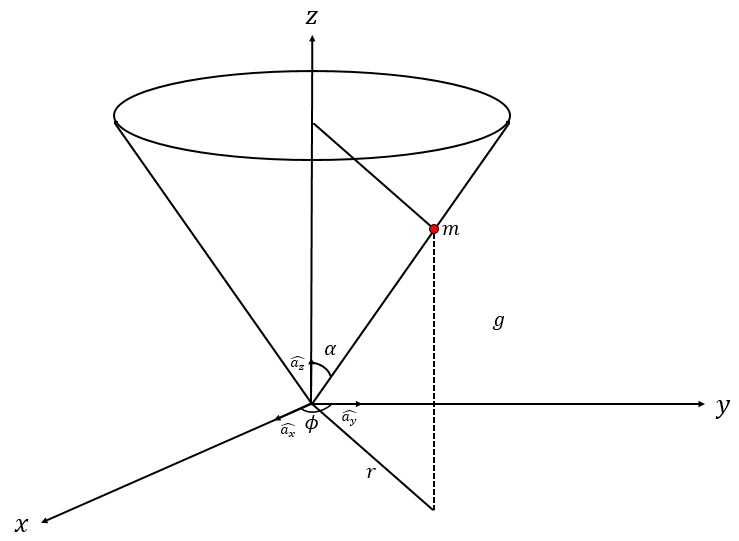
\includegraphics[width=7.01528in,height=5.13568in]{Imagenes/media/image75.jpeg}

Haciendo la transformación de coordenadas se tiene:

\[\cos\phi = \frac{x}{r} \rightarrow x = r\cos\phi\]

\[{sen}\phi = \frac{y}{r} \rightarrow y = r{sen}\phi\]

Para conocer \(z\), se utiliza el ángulo \(\alpha\), por lo que:

\[\cot\alpha = \frac{z}{r} \rightarrow z = r\cot\alpha\]

De esta forma:

\[\dot{x} = \dot{r}\cos\phi - r\dot{\phi}{sen}\phi,\ \ \ \ \ \ \ \ \ \ \dot{y} = \dot{r}{sen}\phi + r\dot{\phi}\cos\phi,\ \ \ \ \ \ \ \ \ \ \dot{z} = \dot{r}\cot\alpha\]

Además, la energía potencial está dada por:

\[U = mgz = mgr\cot\alpha\]

Por otro lado, la velocidad para este sistema viene dada por:

\[{\dot{x}}^{2} = {\dot{r}}^{2}\cos^{2}\phi - 2\dot{r}r\dot{\phi}{\cos\phi sen}\phi + r^{2}\dot{\phi^{2}}{sen}^{2}\phi\]

\[{\dot{y}}^{2} = {\dot{r}}^{2}{sen}^{2}\phi + 2\dot{r}r\dot{\phi}{\cos\phi sen}\phi + r^{2}\dot{\phi^{2}}\cos^{2}\phi\]

\[{\dot{x}}^{2} + {\dot{y}}^{2} = {\dot{r}}^{2} + r^{2}{\dot{\phi}}^{2}\]

Luego el Lagrangiano es:

\[L = \frac{1}{2}m\left( {\dot{r}}^{2} + r^{2}{\dot{\phi}}^{2} + {\dot{r}}^{2}\cot^{2}\alpha \right) - mgr\cot\alpha\]

\[L = \frac{1}{2}m\left\lbrack {\dot{r}}^{2}\left( 1 + \cot^{2}\alpha \right) + r^{2}{\dot{\phi}}^{2} \right\rbrack - mgr\cot\alpha\]

\[L = \frac{1}{2}m\left\lbrack {\dot{r}}^{2}\csc^{2}\alpha + r^{2}{\dot{\phi}}^{2} \right\rbrack - mgr\cot\alpha\]

Ahora se procede a obtener los momentos conjugados \(P_{r}\) y
\(P_{\phi}\), así:

\[p_{r} = \frac{\partial L}{\partial\dot{r}} = m\dot{r}\csc^{2}\alpha\]

\[p_{\phi} = \frac{\partial L}{\partial\dot{\phi}} = mr^{2}\dot{\phi}\]

El Hamiltoniano es:

\[H = \dot{r}p_{r} + \dot{\phi}p_{\phi} - \frac{1}{2}m{\dot{r}}^{2}\csc^{2}\alpha - \frac{1}{2}mr^{2}{\dot{\phi}}^{2} + mgr\cot\alpha\]

\[H\left( r,P_{r},P_{\phi} \right) = \frac{p_{r}^{\ 2}}{2m\csc^{2}\alpha} + \frac{p_{\phi}p_{\phi}}{2mr^{2}} + mgr\cot\alpha = cte\]

Asimismo:

\[{\dot{q}}_{j} = \frac{\partial H}{\partial p_{j}},\ \ \ \ \ \ \ \ \ \ \ {\dot{p}}_{j} = - \frac{\partial H}{\partial q_{j}},\ \ \ \ \ \ \ \ \ \ \dot{r} = \frac{\partial H}{\partial p_{r}} = \frac{p_{r}}{m\csc^{2}\alpha},\ \ \ \ \ \ \ \ \ \ \dot{\phi} = \frac{\partial H}{\partial p_{\phi}} = \frac{p_{\phi}}{mr^{2}}\]

\[{\dot{p}}_{\phi} = - \frac{\partial H}{\partial\phi} = 0,\ \ \ \ \ \ \ \ \ \frac{d}{dt}\left( p_{\phi} \right) = 0,\ \ \ \ \ \ \ \ \ \ p_{\phi} = cte\]

\[\mathbf{m}\mathbf{r}^{\mathbf{2}}\dot{\mathbf{\phi}}\mathbf{= cte}\]

\textbf{Ejemplo 11:} Un partícula \(m\) se desliza sin fricción en el
interior de una superficie o cuenca semiesférica de radio \(R\), que
tiene su eje paralelo al campo gravitacional. Utilice el ángulo polar
\(\theta\) y el ángulo azimutal \(\phi\) para describir la localización
de la partícula.

\begin{enumerate}
\def\labelenumi{\alph{enumi})}
\item
  \begin{quote}
  Hallar el Lagrangiano del sistema.
  \end{quote}
\item
  \begin{quote}
  Hallar \(P_{\theta}\) y \(P_{\phi}\).
  \end{quote}
\item
  \begin{quote}
  Hallar \(H\) y resolver las ecuaciones de movimiento de Hamilton.
  \end{quote}
\item
  \begin{quote}
  Combinar las ecuaciones con el fin de producir una ecuación
  diferencial de segundo orden para \(\theta\) como función del tiempo.
  \end{quote}
\item
  \begin{quote}
  Si \(\theta = \theta_{0}\) y \(\dot{\theta} = 0\) son independientes
  del tiempo. Hallar la velocidad.
  \end{quote}
\item
  \begin{quote}
  Si en \(t = 0\), \(\theta = \theta_{0}\), \(\dot{\theta} = 0\) y
  \(\dot{\phi} = 0\). Hallar la velocidad máxima en momentos
  posteriores.
  \end{quote}
\end{enumerate}

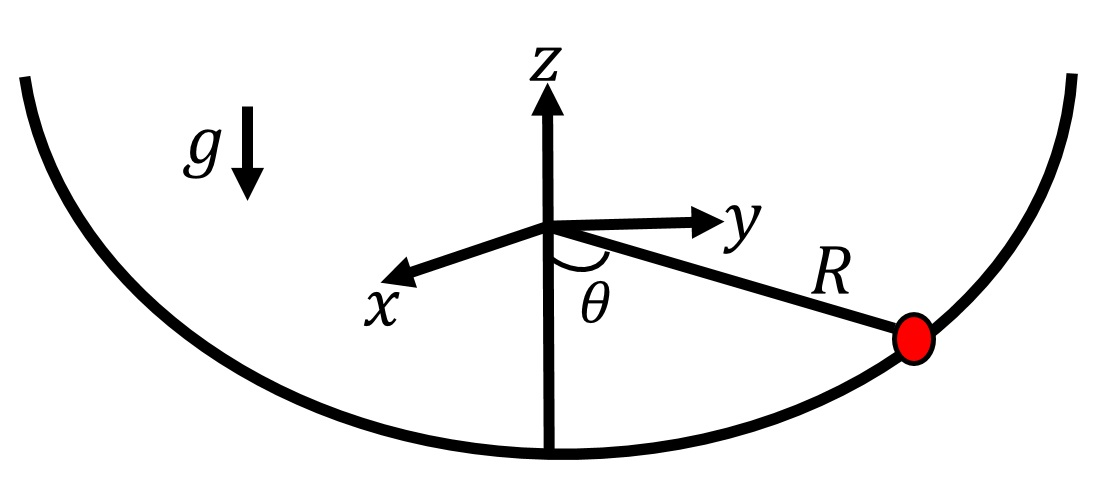
\includegraphics[width=6.78333in,height=2.97917in]{Imagenes/media/image76.jpeg}\textbf{Solución:}
Para la solución de este problema, considérese el siguiente esquema:

a) En coordenadas esféricas, se da que:

\(\overrightarrow{\dot{r}} = \dot{r}\widehat{a_{r}} + r\dot{\theta}\widehat{a_{\theta}} + r{sen}\theta\dot{\phi}\widehat{a_{\phi}}\)

Como el Lagrangiano está dado por \(L = T - U\) y
\(U = - mgR\cos\theta\), entonces:

\[\mathbf{L =}\frac{\mathbf{1}}{\mathbf{2}}\mathbf{m}\mathbf{R}^{\mathbf{2}}\left( \mathbf{sen}^{\mathbf{2}}\mathbf{\theta}{\dot{\mathbf{\phi}}}^{\mathbf{2}} \right)\mathbf{+}\mathbf{mgR}\mathbf{\cos}\mathbf{\theta}\]

b) Para obtener \(p_{\theta}\) y \(p_{\phi}\) se tiene de la ecuación de
movimiento de Lagrange que:

\[\frac{d}{dt}\left( \frac{\partial L}{\partial{\dot{q}}_{j}} \right) - \frac{dL}{dq_{j}} = 0\]

Como:

\[\frac{\partial L}{\partial{\dot{q}}_{j}} = p_{j}\]

Entonces:

\[\mathbf{p}_{\mathbf{\theta}}\mathbf{=}\frac{\mathbf{\partial L}}{\mathbf{\partial}\dot{\mathbf{\theta}}}\mathbf{= m}\mathbf{R}^{\mathbf{2}}\dot{\mathbf{\theta}}\]

\[\mathbf{p}_{\mathbf{\phi}}\mathbf{=}\frac{\mathbf{\partial L}}{\mathbf{\partial}\dot{\mathbf{\phi}}}\mathbf{= m}\mathbf{R}^{\mathbf{2}}{\mathbf{se}\mathbf{n}^{\mathbf{2}}}\mathbf{\theta}\dot{\mathbf{\phi}}\]

c) Para obtener el Hamiltoniano se sabe que:

\[H = T + U\]

\[H\left( q_{j},P_{j};t \right) = \sum_{j}^{}{{\dot{q}}_{j}P_{j} - L\left( q_{j},{\dot{q}}_{j};t \right)}\]

Utilizando la transformación lineal de Legendre:

\[H\left( q_{j},P_{j};t \right) = \dot{\theta}P_{\theta} + \dot{\phi}P_{\theta} - \frac{1}{2}mR^{2}{sen}^{2}\theta{\dot{\phi}}^{2} - \frac{1}{2}mR^{2}{\dot{\theta}}^{2} - mgR\cos\theta\]

Del inciso b) se tiene que:

\[\dot{\theta} = \frac{P_{\theta}}{mR^{2}}\ \ \ \ \ \ \ \ \ \ \ y\ \ \ \ \ \ \ \ \ \ \ \dot{\phi} = \frac{P_{\phi}}{mR^{2}{sen}^{2}\theta\ }\]

De esta manera:

\[H\left( q_{j},P_{j};t \right) = \frac{P_{\theta}^{\ \ 2}}{mR^{2}} + \frac{P_{\phi}^{\ \ 2}}{mR^{2}{sen}^{2}\theta\ } - \frac{1}{2}\frac{mR^{2}{sen}^{2}\theta P_{\phi}^{\ \ 2}}{m^{2}R^{4}{sen}^{4}\theta} - \frac{1}{2}\frac{mR^{2}P_{\phi}^{\ \ 2}}{m^{2}R^{4}} - mgR\cos\theta\]

\[H\left( q_{j},P_{j};t \right) = \frac{1}{2}\frac{P_{\theta}^{\ \ 2}}{mR^{2}} + \frac{1}{2}\frac{P_{\phi}^{\ \ 2}}{mR^{2}{sen}^{2}\theta\ } - mgR\cos\theta\]

\[\mathbf{H}\left( \mathbf{q}_{\mathbf{j}}\mathbf{,}\mathbf{P}_{\mathbf{j}}\mathbf{;t} \right)\mathbf{=}\frac{\mathbf{1}}{\mathbf{2}\mathbf{m}\mathbf{R}^{\mathbf{2}}}\left( \mathbf{P}_{\mathbf{\theta}}^{\mathbf{\ \ 2}}\mathbf{+}\frac{\mathbf{P}_{\mathbf{\phi}}^{\mathbf{\ \ 2}}}{\mathbf{sen}^{\mathbf{2}}\mathbf{\theta}\mathbf{\ }} \right)\mathbf{- mgR}\mathbf{\cos}\mathbf{\theta}\]

Una vez obtenido el Hamiltoniano, se procede a resolver las ecuaciones,
de esta manera:

\[{\dot{q}}_{j} = \frac{\partial H}{\partial P_{j}},\ \ \ \ \ \ \ \ \ \ {- \dot{P}}_{j} = \frac{\partial H}{\partial q_{j}}\]

\[\ \ {- \dot{P}}_{\theta} = \frac{\partial H}{\partial\theta} = \frac{1}{2mR^{2}}\left( - \frac{2{\cos\theta P}_{\phi}^{\ \ 2}}{{sen}^{3}\theta\ } \right) + mgR{sen}\theta\]

\[{\dot{\mathbf{P}}}_{\mathbf{\theta}}\mathbf{=}\frac{\mathbf{P}_{\mathbf{\phi}}^{\mathbf{\ \ 2}}\mathbf{\cos}\mathbf{\theta}}{\mathbf{m}\mathbf{R}^{\mathbf{2}}\mathbf{sen}^{\mathbf{3}}\mathbf{\theta}\mathbf{\ }}\mathbf{- mgR}\mathbf{sen}\mathbf{\theta}\]

Por otro lado, para \({\dot{P}}_{\phi}:\)

\[- {\dot{P}}_{\phi} = \frac{\partial H}{\partial\phi} = 0,\ \ \ \ \ \ \ \ \ \ \frac{dP_{\phi}}{dt} = 0,\ \ \ \ \ \ \ \ \ \ P_{\phi} = cte\]

\[\mathbf{m}\mathbf{R}^{\mathbf{2}}\mathbf{sen}^{\mathbf{2}}\mathbf{\theta}\dot{\mathbf{\phi}}\mathbf{= cte}\]

\[\mathbf{P}_{\mathbf{\theta}}\mathbf{= m}\mathbf{R}^{\mathbf{2}}\dot{\mathbf{\theta}}\]

\[\mathbf{P}_{\mathbf{\phi}}\mathbf{= m}\mathbf{R}^{\mathbf{2}}\mathbf{sen}^{\mathbf{2}}\mathbf{\theta}\dot{\mathbf{\phi}}\]

d) Al combinar las ecuaciones con la finalidad de obtener una ecuación
diferencial de segundo orden para \(\theta\), se tiene:

\[\ddot{\theta} = \frac{1}{mR^{2}}{\dot{P}}_{\theta}\]

\[\ddot{\mathbf{\theta}}\mathbf{=}\frac{\mathbf{1}}{\mathbf{m}\mathbf{R}^{\mathbf{2}}}\left( \frac{\mathbf{P}_{\mathbf{\phi}}^{\mathbf{\ \ 2}}\mathbf{\cos}\mathbf{\theta}}{\mathbf{m}\mathbf{R}^{\mathbf{2}}\mathbf{sen}^{\mathbf{3}}\mathbf{\theta}\mathbf{\ }}\mathbf{- mgR}\mathbf{sen}\mathbf{\theta} \right)\]

e) Para obtener la velocidad con \(\theta = \theta_{0}\) y
\(\dot{\theta} = 0\) independientes de tiempo se tiene:

\[\frac{1}{mR^{2}}\left( \frac{P_{\phi}^{\ \ 2}\cos\theta_{0}}{mR^{2}{sen}^{3}\theta_{0}\ } - mgR{sen}\theta_{0} \right) = 0\]

\[P_{\phi}^{\ \ 2}\cos\theta = m^{2}gR^{3}{sen}^{4}\theta_{0}\]

\[m^{2}R^{4}{sen}^{4}\theta_{0}\cos\theta_{0}{\dot{\phi}}^{2} = m^{2}gR^{3}{sen}^{4}\theta_{0}\]

\[{\dot{\mathbf{\phi}}}^{\mathbf{2}}\mathbf{= \pm}\sqrt{\frac{\mathbf{g}}{\mathbf{R}\mathbf{\cos}\mathbf{\theta}_{\mathbf{0}}}}\]

Los signos \(\pm\) indican las direcciones horaria y antihoraria de la
velocidad.

f) Como en \(t = 0\), \(\dot{\phi} = 0\),
\(\dot{\phi}mR^{2}{sen}\theta = P_{\phi} = 0\), entonces:

\[\ddot{\mathbf{\theta}}\mathbf{= -}\frac{\mathbf{g}}{\mathbf{R}}\mathbf{sen}\mathbf{\theta}\]

La expresión anterior es la ecuación de movimiento de un péndulo, como
es un sistema conservativo \(H = cte\), por lo que:

\[H(t) = H(0)\]

Es decir:

\[H(t) = \frac{1}{2mR^{2}}\left( P_{\theta}^{\ \ 2} + \frac{P_{\phi}^{\ \ 2}}{{sen}^{2}\theta\ } \right) - mgR\cos\theta\]

En este caso:

\[\frac{P_{\phi}^{\ \ 2}}{{sen}^{2}\theta\ } = 0\]

De este modo:

\[H(t) = \frac{1}{2mR^{2}}m^{2}R^{4}{\dot{\theta}}^{2} - mgR\cos\theta\]

\[H(t) = - mgR{\cos\theta}_{0}\]

De esta manera:

\[\frac{mR^{2}{\dot{\theta}}^{2}}{2} = mgR\left( \cos\theta - {\cos\theta}_{0} \right)\]

Despejando \(\dot{\theta}:\)

\[\dot{\mathbf{\theta}}\mathbf{=}\sqrt{\frac{\mathbf{2}\mathbf{g}}{\mathbf{R}}}\left( \mathbf{\cos}\mathbf{\theta}\mathbf{-}{\mathbf{\cos}\mathbf{\theta}}_{\mathbf{0}} \right)\]

La velocidad es máxima en momentos posteriores cuando \(\theta = 0\),
por lo tanto:

\[V_{T} = R\dot{\theta}\]

\[\mathbf{V}_{\mathbf{T}}\mathbf{=}\sqrt{\mathbf{2}\mathbf{gR(1 -}\mathbf{\cos}\mathbf{\theta}}\]

\textbf{SOLUCIÓN ROUTHIANA DE UN SISTEMA DINÁMICO}

La función Routhiana se define como la transformación lineal de Legendre
del Hamiltoniano respecto de las velocidades generalizadas
correspondientes a las coordenadas cíclicas, es decir:

\[R\left( q_{1},\ldots,q_{s},q_{s + 1},\ldots q_{n},p_{1},p_{2},{..p}_{s},{\dot{q}}_{s + 1},\ldots,{\dot{q}}_{n};t \right) = \sum_{j = 1}^{s}{\dot{q}}_{j}p_{j} - L\left( q_{1},\ldots,q_{s},q_{s + 1},\ldots,q_{n},{\dot{q}}_{1}\ldots;t \right)\ \ \ \ \ \ \ \ \ \ \ \]

Donde \(q_{1},\ldots,q_{s}\) son coordenadas cíclicas, \(q_{s + 1}\) es
una coordenada no cíclica y \(p_{1},p,p_{s}\) son los momentos canónicos
asociados a las \(s\) coordenadas cíclicas, de esta manera, obteniendo
el diferencial de la Routhiana, se tiene que:

\(dR = \sum_{j = 1}^{s}{\frac{\partial R}{\partial q_{j}}dq_{j}} + \sum_{j = s + 1}^{n}{\frac{\partial R}{\partial q_{j}^{\ \ *}}dq_{j}} + \sum_{j = 1}^{s}{\frac{\partial R}{\partial p_{j}}dp_{j}} + \sum_{\mathbf{j = s + 1}}^{\mathbf{n}}{\frac{\mathbf{\partial R}}{\mathbf{\partial}{\dot{\mathbf{q}}}_{\mathbf{j}}^{\mathbf{\ \ }}}\mathbf{d}{\dot{\mathbf{q}}}_{\mathbf{j}}} + \frac{\partial R}{\partial t}dt\)

\[dR = \sum_{j = 1}^{s}{\dot{q_{j}}dp_{j}} + \sum_{j = 1}^{s}{p_{j}d{\dot{q}}_{j}} - \sum_{j = 1}^{s}\frac{\partial L}{\partial q_{j}}dq_{j} - \sum_{j = s + 1}^{n}\frac{\partial L}{\partial q_{j}}dq_{j} - \sum_{j = 1}^{s}\frac{\partial L}{\partial{\dot{q}}_{j}}d{\dot{q}}_{j} - \sum_{\mathbf{j = s + 1}}^{\mathbf{n}}\frac{\mathbf{\partial L}}{\mathbf{\partial}{\dot{\mathbf{q}}}_{\mathbf{j}}}\mathbf{d}{\dot{\mathbf{q}}}_{\mathbf{j\ }} - \frac{\partial L}{\partial t}dt\]

De la ecuación de movimiento de Lagrange se cumple que:

\[\frac{d}{dt}\left( \frac{\partial L}{\partial\dot{q_{j}}} \right) - \frac{\partial L}{\partial q_{j}} = 0,\ \ \ \ \ \ \ \ \ \ \frac{\partial L}{\partial{\dot{q}}_{j}} = p_{j},\ \ \ \ \ \ \ \ \ \ {\dot{p}}_{j} = \frac{\partial L}{\partial q_{j}}\]

Y para este caso:

\[{\dot{\mathbf{q}}}_{\mathbf{j}}\mathbf{=}\frac{\mathbf{\partial R}}{\mathbf{\partial}\mathbf{p}_{\mathbf{j}}}\]

\[\mathbf{-}\mathbf{p}_{\mathbf{j}}\mathbf{=}\frac{\mathbf{\partial R}}{\mathbf{\partial}\mathbf{q}_{\mathbf{j}}}\]

\[\frac{\mathbf{\partial R}}{\mathbf{\partial t}}\mathbf{= -}\frac{\mathbf{\partial L}}{\mathbf{\partial t}}\]

Las ecuaciones (195), (196) y (197) corresponden a las ecuaciones de
movimiento de Hamilton con la Routhiana haciendo el papel de
Hamiltoniano para las coordenadas cíclicas.

A continuación, se va a mostrar que las ecuaciones anteriores satisfacen
la ecuación de movimiento de Lagrange, esto es:

\[\frac{\partial R}{\partial q_{j}} = - \frac{\partial L}{\partial q_{j}}\ \ \ \ \ \ \ \ \ \]

\[\frac{\partial R}{\partial{\dot{q}}_{j}} = - \frac{\partial L}{\partial{\dot{q}}_{j}}\ \ \ \ \ \ \ \ \ \ \]

Llevando las ecuaciones anteriores a la ecuación de movimiento de
Lagrange, entonces:

\[\frac{d}{dt}\left( \frac{\partial L}{\partial\dot{q_{j}}} \right) - \frac{\partial L}{\partial q_{j}} = 0\]

\[- \frac{d}{dt}\left( \frac{\partial R}{\partial\dot{q_{j}}} \right) + \frac{\partial R}{\partial q_{j}} = 0\]

\[\frac{d}{dt}\left( \frac{\partial R}{\partial\dot{q_{j}}} \right) - \frac{\partial R}{\partial q_{j}} = 0\]

Del Principio de Mínima Acción de Hamilton Modificado \(q_{j}\) y
\(p_{j}\) son independientes, por lo que se hace necesario encontrar una
transformación para hacer que las coordenadas generalizadas no cíclicas,
se vuelvan cíclicas, de esta manera se introduce la coordenada
\(Q_{j}\), lo que conlleva a que \(Q_{j}\) y \(P_{j}\) deben ser
coordenadas cíclicas, para esto se define una nueva coordenada
dependiente de \(Q_{j}\), \(P_{j}\) y \(t\), por lo tanto:

\[Q_{j = (q_{j},p_{j};t)}\]

\[P_{j = (q_{j},p_{j};t)}\]

Las Q\textsubscript{j y} P\textsubscript{j}, son las coordenadas que son
cíclicas y los momentos asociados a dichas coordenadas.

\[K = K\left( Q_{j},P_{j};t \right)\]

De este modo:

\[{\dot{Q}}_{j} = \frac{\partial K}{\partial P_{j}},\ \ \ \ \ \ \ \ \  - {\dot{P}}_{j} = \frac{\partial K}{\partial Q_{j}}\]

Por lo tanto existe un nuevo Hamiltoniano de la forma:

\hypertarget{mathbfkmathbf-mathbfkleft-mathbfq_mathbfjmathbfmathbfp_mathbfjmathbfmathbft-right}{%
\section{\texorpdfstring{ \(\mathbf{K}\mathbf{=}\)
\(\mathbf{K}\left( \mathbf{Q}_{\mathbf{j}}\mathbf{,}\mathbf{P}_{\mathbf{j}}\mathbf{;}\mathbf{t} \right)\)}{ \textbackslash mathbf\{K\}\textbackslash mathbf\{=\} \textbackslash mathbf\{K\}\textbackslash left( \textbackslash mathbf\{Q\}\_\{\textbackslash mathbf\{j\}\}\textbackslash mathbf\{,\}\textbackslash mathbf\{P\}\_\{\textbackslash mathbf\{j\}\}\textbackslash mathbf\{;\}\textbackslash mathbf\{t\} \textbackslash right)}}\label{mathbfkmathbf-mathbfkleft-mathbfq_mathbfjmathbfmathbfp_mathbfjmathbfmathbft-right}}

Por lo que simultáneamente las \(Q_{j}\) y \(P_{j}\) deben cumplir el
Principio de Mínima Acción de Hamilton Modificado, por lo tanto:

\[\delta\int_{t_{1}}^{t_{2}}{\left\lbrack \sum_{j}^{}{P_{j}{\dot{Q}}_{j} - \ \ \ \ K\left( Q_{j},P_{j};t \right)} \right\rbrack\ dt} = 0\]

Asimismo, debe cumplirse que:

\[L^{,} = L + \frac{dF}{dt}\]

δS=δS\textsuperscript{,}

\[\delta\int_{t_{1}}^{t_{2}}{\left\lbrack \sum_{j}^{}{p_{j}{\dot{q}}_{j} - H\left( q_{j},p_{j};t \right)} \right\rbrack\ dt} = 0\]

Esto conlleva a que:

\[\int_{t_{1}}^{t_{2}}{\ \frac{dF}{dt}}dt = F\left( t_{2} \right) - F\left( t_{2} \right) = 0\]

Por lo que:

\[\sum_{j}^{}{p_{j}{\dot{q}}_{j} - H\left( q_{j},p_{j};t \right)} = \sum_{j}^{}{P_{j}{\dot{Q}}_{j} - \ \ \ \ K\ \left( Q_{j},P_{j};t \right)} + \frac{dF}{dt}\]

\(F\) es la función generalizada de la transformación canónica. La
función generatriz debe ser tal que tenga una coordenada antigua y otra
nueva, para esto considérense las siguientes funciones generatrices:

\[F_{1} = F_{1}\left( q_{j},Q_{j};t \right),\ \ \ \ \ \ \ \ \ \ F_{2} = F_{2}\left( q_{j},P_{j};t \right),\ \ \ \ \ \ \ \ \ \ F_{3} = F_{3}\left( p_{j},Q_{j};t \right),\ \ \ \ \ \ \ \ \ \ F_{4} = F_{4}\left( p_{j},P_{j};t \right)\]

En caso de que la función generatriz sea
\(F_{1} = F_{1}\left( q_{j},Q_{j};t \right)\):

\[\sum_{j}^{}{p_{j}{\dot{q}}_{j} - H\left( q_{j},p_{j};t \right)} = \sum_{j}^{}{P_{j}{\dot{Q}}_{j} - K\left( Q_{j},P_{j};t \right)} + \frac{dF_{1}\left( q_{j},Q_{j};t \right)}{dt}\]

\[\sum_{j}^{}{p_{j}{\dot{q}}_{j} - H\left( q_{j},p_{j};t \right)} = \sum_{j}^{}{P_{j}{\dot{Q}}_{j} - K} + \sum_{j}^{}{\frac{\partial F_{1}}{\partial q_{j}}{\dot{q}}_{j}} + \sum_{j}^{}{\frac{\partial F_{1}}{\partial Q_{j}}{\dot{Q}}_{j}} + \frac{\partial F_{1}}{\partial t}\]

\[\sum_{j}^{}\left( P_{j} + \frac{\partial F_{1}}{\partial Q_{j}} \right){\dot{Q}}_{j} + \sum_{j}^{}\left( \frac{\partial F_{1}}{\partial q_{j}} - p_{j} \right){\dot{q}}_{j} + H - K + \frac{\partial F_{1}}{\partial t} = 0\ \ \ \ \ \ \]

En la ecuación (201) se da que \({\dot{Q}}_{j}\) es independiente y
\({\dot{q}}_{j}\) es dependiente. Por otro lado:

\[\mathbf{P}_{\mathbf{j}}\mathbf{= -}\frac{\mathbf{\partial}\mathbf{F}_{\mathbf{1}}\left( \mathbf{q}_{\mathbf{j}}\mathbf{,}\mathbf{Q}_{\mathbf{j}}\mathbf{;t} \right)}{\mathbf{\partial}\mathbf{Q}_{\mathbf{j}}}\mathbf{,\ \ \ \ \ \ \ \ \ \ \ }\mathbf{p}_{\mathbf{j}}\mathbf{=}\frac{\mathbf{\partial}\mathbf{F}_{\mathbf{1}}\left( \mathbf{q}_{\mathbf{j}}\mathbf{,}\mathbf{Q}_{\mathbf{j}}\mathbf{;t} \right)}{\mathbf{\partial}\mathbf{q}_{\mathbf{j}}}\]

\[H - K + \frac{\partial F_{1}}{\partial t} = 0\]

\[K = H + \frac{\partial F_{1}}{\partial t}\]

Hay \(n\) transformaciones para \(Q_{j}\) y \(n\) transformaciones para
\(P_{j}\), así que hay \(2n\) transformaciones cuando se utiliza como
función generatriz \(F_{1} = F_{1}\left( q_{j},Q_{j};t \right)\).

Si la función generatriz es
\(F_{2} = F_{2}\left( q_{j},P_{j};t \right)\), se parte de:

\[P_{j} = - \frac{\partial F_{1}\left( q_{j},Q_{j};t \right)}{\partial Q_{j}}\]

\[\int_{}^{}{P_{j}\partial Q_{j} = - \int_{}^{}{\partial F_{1}\left( q_{j},Q_{j};t \right)}}\]

Por lo que:

\[\sum_{j}^{}{P_{j}Q_{j} + F_{1}}\left( q_{j},Q_{j};t \right) = F_{2}\left( q_{j},P_{j};t \right)\]

\[\sum_{j}^{}{p_{j}{\dot{q}}_{j} - H\left( q_{j},p_{j};t \right)} = \sum_{j}^{}{P_{j}{\dot{Q}}_{j} - K} + \frac{d}{dt}\left\lbrack F_{2}\left( q_{j},P_{j};t \right) - \sum_{j}^{}{P_{j}Q_{j}} \right\rbrack\]

\[\sum_{j}^{}{p_{j}{\dot{q}}_{j} - H} = \sum_{j}^{}{P_{j}{\dot{Q}}_{j} - K} + \sum_{j}^{}{\frac{\partial F_{2}}{dq_{j}}{\dot{q}}_{j}} + \sum_{j}^{}{\frac{\partial F_{2}}{dP_{j}}{\dot{P}}_{j}} + \frac{\partial F_{2}}{\partial t} - \sum_{j}^{}{P_{j}{\dot{Q}}_{j}} - \sum_{j}^{}{{\dot{P}}_{j}Q_{j}}\]

\[\sum_{j}^{}\left( \frac{\partial F_{2}}{\partial q_{j}} - p_{j} \right){\dot{q}}_{j} + \sum_{j}^{}\left( \frac{\partial F_{2}}{\partial P_{j}} - Q_{j} \right){\dot{P}}_{j} + H - K + \frac{\partial F_{2}}{\partial t} = 0\ \ \ \ \ \ \]

En la ecuación (202) también se da que hay \(n\) transformaciones para
\(P_{j}\) y \(n\) transformaciones para \(Q_{j}\), es decir:

\[\mathbf{p}_{\mathbf{j}}\mathbf{=}\frac{\mathbf{\partial}\mathbf{F}_{\mathbf{2}}\left( \mathbf{q}_{\mathbf{j}}\mathbf{,}\mathbf{P}_{\mathbf{j}}\mathbf{;t} \right)}{\mathbf{\partial}\mathbf{q}_{\mathbf{j}}}\mathbf{,\ \ \ \ \ \ \ \ \ \ \ }\mathbf{Q}_{\mathbf{j}}\mathbf{=}\frac{\mathbf{\partial}\mathbf{F}_{\mathbf{2}}\left( \mathbf{q}_{\mathbf{j}}\mathbf{,}\mathbf{P}_{\mathbf{j}}\mathbf{;t} \right)}{\mathbf{\partial}\mathbf{P}_{\mathbf{j}}}\]

\[K = H + \frac{\partial F_{2}}{\partial t}\]

\[F_{1} = F_{1}\left( q_{j},Q_{j};t \right)\]

Si la función generatriz es
\(F_{3} = F_{3}\left( p_{j},Q_{j};t \right)\), se parte de:

\[\mathbf{p}_{\mathbf{j}}\mathbf{=}\frac{\mathbf{\partial}\mathbf{F}_{\mathbf{1}}\left( \mathbf{q}_{\mathbf{j}}\mathbf{,}\mathbf{Q}_{\mathbf{j}}\mathbf{;t} \right)}{\mathbf{\partial}\mathbf{q}_{\mathbf{j}}}\]

\[\int_{}^{}{P_{j}\partial q_{j} = \int_{}^{}{\partial F_{1}\left( q_{j},Q_{j};t \right)}}\]

Como la integral es una suma de Riemann, entonces:

\[F_{1}\left( q_{j},Q_{j};t \right) = F_{3}\left( p_{j},Q_{j};t \right) + \sum_{j}^{}{p_{j}q_{j}}\]

Además:

\[\sum_{j}^{}{p_{j}{\dot{q}}_{j} - H\left( q_{j},p_{j};t \right)} = \sum_{j}^{}{P_{j}{\dot{Q}}_{j}} - K + \sum_{j}^{}\frac{\partial F_{3}}{\partial p_{j}}{\dot{p}}_{j} + \sum_{j}^{}\frac{\partial F_{3}}{\partial Q_{j}}{\dot{Q}}_{j} + \frac{\partial F_{3}}{\partial t} + \sum_{j}^{}p_{j}{\dot{q}}_{j} + \sum_{j}^{}q_{j}{\dot{p}}_{j}\]

\[\sum_{j}^{}\left( P_{j} + \frac{\partial F_{3}}{\partial Q_{j}} \right){\dot{Q}}_{j} + \sum_{j}^{}\left( \frac{\partial F_{3}}{\partial p_{j}} + q_{j} \right){\dot{p}}_{j} + H - K + \frac{\partial F_{3}}{\partial t} = 0\ \ \ \ \ \ \]

\[\mathbf{P}_{\mathbf{j}}\mathbf{= -}\frac{\mathbf{\partial}\mathbf{F}_{\mathbf{3}}\left( \mathbf{P}_{\mathbf{j}}\mathbf{,}\mathbf{Q}_{\mathbf{j}}\mathbf{;t} \right)}{\mathbf{\partial}\mathbf{Q}_{\mathbf{j}}}\mathbf{,\ \ \ \ \ \ \ \ \ \ \ }\mathbf{q}_{\mathbf{j}}\mathbf{= -}\frac{\mathbf{\partial}\mathbf{F}_{\mathbf{3}}\left( \mathbf{P}_{\mathbf{j}}\mathbf{,}\mathbf{Q}_{\mathbf{j}}\mathbf{;t} \right)}{\mathbf{\partial}\mathbf{p}_{\mathbf{j}}}\]

\[K = H + \frac{\partial F_{3}}{\partial t}\]

Si la función generatriz es
\(F_{4} = F_{4}\left( p_{j},P_{j};t \right)\), hay que notar que existe
una nueva coordenada \(p_{j}\), por lo que:

\[\sum_{j}^{}\left( \frac{\partial F_{4}}{\partial P_{j}} + q_{j} \right){\dot{P}}_{j} + \sum_{j}^{}\left( \frac{\partial F_{4}}{\partial P_{j}} - Q_{j} \right){\dot{P}}_{j} + H - \kappa + \frac{\partial F_{4}}{\partial t} = 0\ \ \ \ \ \ \ \ \ \]

\[\mathbf{q}_{\mathbf{j}}\mathbf{= -}\frac{\mathbf{\partial}\mathbf{F}_{\mathbf{4}}\left( \mathbf{p}_{\mathbf{j}}\mathbf{,}\mathbf{P}_{\mathbf{j}}\mathbf{;t} \right)}{\mathbf{\partial}\mathbf{p}_{\mathbf{j}}}\mathbf{,\ \ \ \ \ \ \ \ \ \ \ }\mathbf{Q}_{\mathbf{j}}\mathbf{= -}\frac{\mathbf{\partial}\mathbf{F}_{\mathbf{4}}\left( \mathbf{P}_{\mathbf{j}}\mathbf{,}\mathbf{P}_{\mathbf{j}}\mathbf{;t} \right)}{\mathbf{\partial}\mathbf{P}_{\mathbf{j}}}\]

Aplicando las transformaciones lineales a un sistema termodinámico, para
esto se sabe que el cambio de la energía interna de un sistema viene
dada por:

\[du = \delta q - \delta W_{ext}\ \ \ \ \]

Por otro lado, también se sabe que el cambio de la entropía viene dado
por:

\[ds = \frac{\delta q_{rev}}{T} + \frac{\delta q_{no\ rev}}{T}\]

De esta manera (205) toma la forma:

\[u = u(s,V)\]

\(du = Tds - PdV\)

\[du = \left( \frac{\partial U}{\partial s} \right)_{V}ds + \left( \frac{\partial U}{\partial V} \right)_{s}dV\]

De la ecuación (206) se tiene entonces que:

\[\left( \frac{\mathbf{\partial u}}{\mathbf{\partial s}} \right)_{\mathbf{V}}\mathbf{= T,}\mathbf{\ \ \ \ \ \ \ \ \ \ }\left( \frac{\mathbf{\partial u}}{\mathbf{\partial V}} \right)_{\mathbf{s}}\mathbf{= - P}\]

Ahora se sabe que la entalpía está dada por:

\[H = u + PV\]

Por lo que:

\[dH = d(u + PV)\]

\[dH = du + PdV + VdP\]

\[dH = TdS - PdV + PdV + VdP\]

\[dH = TdS + VdP\]

De esta manera, la función de entalpía, toma la forma:

\[H = H(s,P)\]

Por lo que (207) es entonces:

\[dH = \left( \frac{\partial H}{\partial s} \right)_{p}ds + \left( \frac{\partial H}{\partial P} \right)_{s}dP\]

Y de (208):

\[\left( \frac{\mathbf{\partial H}}{\mathbf{\partial s}} \right)_{\mathbf{p}}\mathbf{= T,\ \ \ \ \ \ \ \ \ \ \ \ }\left( \frac{\mathbf{\partial H}}{\mathbf{\partial P}} \right)_{\mathbf{s}}\mathbf{= V}\]

Ahora, para la energía de Helmholtz, se tiene que esta viene dada por:

\[F = u - Ts\]

Así:

\[dF = d(u - Ts)\]

\[dF = du - Tds - sdT\]

\[dF = TdS - PdV - Tds - sdT\]

\[dF = - PdV - sdT\]

De esta manera, la función para la energía de Helmholtz, toma la forma:

\[F = F(V,T)\]

Por lo que (209) es entonces:

\[dF = \left( \frac{\partial F}{\partial V} \right)_{T}dV + \left( \frac{\partial F}{\partial T} \right)_{V}dT\]

Y de (210):

\[\left( \frac{\mathbf{\partial F}}{\mathbf{\partial V}} \right)_{\mathbf{T}}\mathbf{= - P,\ \ \ \ \ \ \ \ \ \ \ \ }\left( \frac{\mathbf{\partial F}}{\mathbf{\partial T}} \right)_{\mathbf{V}}\mathbf{= - s}\]

Por último, para la energía de Gibbs, se tiene que:

\[G = u - Ts + PV\]

Así:

\[dG = d(u - Ts + PV)\]

\[dG = du - Tds - sdT + PdV + VdP\]

\[dG = PdV + VdP + TdS - PdV - Tds - sdT\]

\[dG = - sdT + VdP\]

De esta manera, la función para la energía de Gibbs, toma la forma:

\[G = G(T,P)\]

Por lo que (211) es entonces:

\[dG = \left( \frac{\partial G}{\partial T} \right)_{P}dT + \left( \frac{\partial G}{\partial P} \right)_{T}dP\]

Y de (212):

\[\left( \frac{\mathbf{\partial G}}{\mathbf{\partial T}} \right)_{\mathbf{P}}\mathbf{= - s,\ \ \ \ \ \ \ \ \ \ \ \ }\left( \frac{\mathbf{\partial G}}{\mathbf{\partial P}} \right)_{\mathbf{T}}\mathbf{= V}\]

0

\textbf{Ejemplo 14:} Analizar el problema del oscilador armónico
utilizando la función generatriz:

\[F = \frac{1}{2}m\omega q^{2}\cot Q\]

\[F_{1}(q,Q;t) = \frac{1}{2}m\omega q^{2}\cot Q\]

\textbf{Solución:} De la función generatriz se puede notar que esta no
depende explícitamente del tiempo, de esta manera, se tiene que:

\[\mathbf{P}_{\mathbf{j}}\mathbf{= -}\frac{\mathbf{\partial}\mathbf{F}_{\mathbf{1}}\left( \mathbf{q}_{\mathbf{j}}\mathbf{,}\mathbf{Q}_{\mathbf{j}}\mathbf{;t} \right)}{\mathbf{\partial}\mathbf{Q}_{\mathbf{j}}}\mathbf{,\ \ \ \ \ \ \ \ \ \ \ }\mathbf{p}_{\mathbf{j}}\mathbf{=}\frac{\mathbf{\partial}\mathbf{F}_{\mathbf{1}}\left( \mathbf{q}_{\mathbf{j}}\mathbf{,}\mathbf{Q}_{\mathbf{j}}\mathbf{;t} \right)}{\mathbf{\partial}\mathbf{q}_{\mathbf{j}}}\]

\[p = \frac{\partial F_{1}}{\partial q} = m\omega q\cot Q\]

\[P = - \frac{\partial F_{1}}{\partial Q} = - \frac{1}{2}m\omega q^{2}\left( {- \csc^{2}}Q \right) = \frac{1}{2}\frac{m\omega q^{2}}{{sen}^{2}Q}\]

De esta manera:

\[q^{2} = \frac{2P}{m\omega}{sen}^{2}Q\]

\[\mathbf{q =}\sqrt{\frac{\mathbf{2}\mathbf{P}}{\mathbf{m\omega}}}\mathbf{sen}\mathbf{Q}\]

\[p = m\omega\sqrt{\frac{2P}{m\omega}}{sen}Q\frac{\cos Q}{{sen}Q}\]

\[\mathbf{p =}\sqrt{\frac{\mathbf{m\omega}\mathbf{2}\mathbf{P}}{}}\mathbf{\cos}\mathbf{Q}\]

Por otro lado el Lagrangiano y el Hamiltoniano son:

\[L = \frac{1}{2}m{\dot{q}}^{2} - \frac{1}{2}kq^{2}\]

\[K = \frac{p^{2}}{2m} + \frac{1}{2}kq^{2} + \ \frac{\partial F_{1}}{\partial t}\]

Para este caso el nuevo Hamiltoniano es:

\[K = H\]

\(K(Q,P) = H\)(q \textsubscript{,} p)

Donde \(K\), está dada por:

\[K(Q,P) = \frac{1}{2}m{\dot{q}}^{2} + \frac{1}{2}kq^{2}\]

Escribiendo a \(\kappa\) en términos de \(Q\), \(P\) y \(t\), se hace
necesario que:

\[K(Q,P;t) = \frac{p^{2}}{2m} + \frac{1}{2}kq^{2}\]

Es decir que:

\[K(Q,P,t) = \frac{1}{2m}(2Pm\omega)\cos^{2}Q + \frac{1}{2}m\omega^{2}\left( \frac{2P}{m\omega} \right){sen}^{2}Q\]

\[K(Q,P) = P\omega\left( \cos^{2}Q + {sen}^{2}Q \right) = P\omega = cte\]

Por lo que se dice el nuevo Hamiltoniano es cíclico en \(Q\) y constante
en \(P\), lo que conlleva a un caso de integrales primeras de
movimiento, de este modo:

\[\frac{E}{\omega} = P\]

Finalmente:

\[K = K\left( Q_{j},P_{j};t \right)\]

De este modo:

\[{\dot{Q}}_{j} = \frac{\partial K}{\partial P_{j}},\ \ \ \ \ \ \ \ \  - {\dot{P}}_{j} = \frac{\partial K}{\partial Q_{j}}\]

\[{\dot{Q}}_{} = \frac{\partial K}{\partial P_{}} = \frac{\partial(P\omega)}{\partial P_{}} = \omega\]

\[\frac{dQ}{dt} = \omega\]

\[Q = \omega t + \alpha\]

\[\frac{dP}{dt} = - \frac{\partial\left( \frac{E}{\omega} \right)}{\partial Q} = 0\]

P=cte

\[\mathbf{q =}\sqrt{\frac{\mathbf{2}\mathbf{E}}{\mathbf{m}\mathbf{\omega}^{\mathbf{2}}}}\mathbf{sen}\left( \mathbf{\omega t + \alpha} \right)\]

\[\mathbf{p =}\sqrt{\mathbf{2}\mathbf{Em}}\mathbf{\cos}\left( \mathbf{\omega t + \alpha} \right)\]

\textbf{Ejemplo 15:} Analizar el problema del oscilador armónico simple
amortiguado, usando la función generatriz:

\(F = e^{\frac{b}{2m}t}qP\)

\[F_{2}(q,P;t) = e^{\frac{b}{2m}t}qP\]

\textbf{Solución:} Inicialmente, se sabe que la ecuación diferencial
para un oscilador armónico simple amortiguado es:

\[m\ddot{x} = - b\dot{x} - kx\]

Reescribiéndola:

\[\ddot{x} + \frac{b}{m}\dot{x} + \frac{k}{m}x = 0\]

El Lagrangiano va a estar dado por:

\[L = (T - U)e^{\frac{b}{m}t} = \frac{1}{2}m{\dot{q}}^{2}e^{\frac{b}{m}t} - \frac{1}{2}kq^{2}e^{\frac{b}{m}t}\]

Así:

\[p = \frac{\partial L}{\partial\dot{q}} = m\dot{q}e^{\frac{b}{m}t}\]

Por lo tanto el Hamiltoniano es:

\[H = \frac{p^{2}}{m}e^{- \frac{b}{m}t} - \frac{1}{2}me^{\frac{b}{m}t}\frac{p^{2}}{m^{2}}e^{- \frac{2b}{m}t} + \frac{1}{2}kq^{2}e^{\frac{b}{m}t}\]

\[\mathbf{H}\left( \mathbf{q,p;t} \right)\mathbf{=}\frac{\mathbf{p}^{\mathbf{2}}}{\mathbf{2}\mathbf{m}}\mathbf{e}^{\mathbf{-}\frac{\mathbf{b}}{\mathbf{m}}\mathbf{t}}\mathbf{+}\frac{\mathbf{1}}{\mathbf{2}}\mathbf{k}\mathbf{q}^{\mathbf{2}}\mathbf{e}^{\frac{\mathbf{b}}{\mathbf{m}}\mathbf{t}}\]

Este Hamiltoniano depende explícitamente del tiempo. Ahora, se procede a
analizar la función generatriz:

\[F = e^{\frac{b}{2m}t}qP\]

De tal manera que se pueda ver que el nuevo Hamiltoniano K, no depende
explícitamente del tiempo, así:

\[\mathbf{p}_{\mathbf{j}}\mathbf{=}\frac{\mathbf{\partial}\mathbf{F}_{\mathbf{2}}\left( \mathbf{q}_{\mathbf{j}}\mathbf{,}\mathbf{P}_{\mathbf{j}}\mathbf{;t} \right)}{\mathbf{\partial}\mathbf{q}_{\mathbf{j}}}\mathbf{,\ \ \ \ \ \ \ \ \ \ \ }\mathbf{Q}_{\mathbf{j}}\mathbf{=}\frac{\mathbf{\partial}\mathbf{F}_{\mathbf{2}}\left( \mathbf{q}_{\mathbf{j}}\mathbf{,}\mathbf{P}_{\mathbf{j}}\mathbf{;t} \right)}{\mathbf{\partial}\mathbf{P}_{\mathbf{j}}}\]

\[K = H + \frac{\partial F_{2}}{\partial t}\]

\[\frac{\partial F_{2}(q,P;t)}{\partial t} = e^{\frac{b}{2m}t}\frac{b}{2m}qP\]

\[p = \frac{\partial F_{2}}{\partial q} = e^{\frac{b}{2m}t}P,\ \ \ \ \ \ \ \ \ \ \ \ Q = \frac{\partial F_{2}}{\partial P} = e^{\frac{b}{2m}t}q\]

De este modo, el nuevo Hamiltoniano es:

\[\ \ \ \ \ K = \frac{p^{2}}{2m}e^{- \frac{b}{m}t} + \frac{1}{2}kq^{2}e^{\frac{b}{m}t} + \frac{b}{2m}e^{\frac{b}{2m}t}qP\]

\[\frac{P^{2}}{2m} + \frac{1}{2}kQ^{2} + \frac{b}{2m}QP\]

\[\dot{\mathbf{Q}}\mathbf{=}\frac{\mathbf{\partial K\ \ \ \ }}{\mathbf{\partial P}}\mathbf{=}\frac{\mathbf{P}}{\mathbf{m}}\mathbf{+}\frac{\mathbf{b}}{\mathbf{2}\mathbf{m}}\mathbf{Q,\ \ \ \ \ \ \ \ \ \ \ }\dot{\mathbf{P}}\mathbf{= -}\frac{\mathbf{\partial K\ \ \ \ }}{\mathbf{\partial Q}}\mathbf{= - kQ -}\frac{\mathbf{b}}{\mathbf{2}\mathbf{m}}\mathbf{P}\]

Queda como ejercicio regresar a las antiguas coordenadas y momentos
generalizados. \(\therefore\)

\textbf{CORCHETES DE POISSON Y ÁLGEBRA DE LIE}

Sea una función \(f\) cualquiera definida en el espacio de fase, es
decir:

\[f = f\left( q_{j},p_{j};t \right)\]

Se cumple que:

\[\frac{df}{dt} = \sum_{}^{}\left( \frac{\partial f}{\partial q_{j}}{\dot{q}}_{j} + \frac{\partial f}{\partial p_{j}}{\dot{p}}_{j} \right) + \frac{\partial f}{\partial t}\ \ \ \ \ \ \ \ \]

La ecuación (213) debe cumplir el Principio de Mínima Acción de Hamilton
Modificado, de esta manera:

\[\dot{q_{j}} = \frac{\partial H}{\partial p_{j}},\ \ \ \ \ \ \ \ \  - {\dot{p}}_{j} = \frac{\partial H}{\partial q_{j}}\]

\[\frac{df}{dt} = \sum_{j}^{}{\left( \frac{\partial f}{\partial q_{j}}\frac{\partial H}{\partial p_{j}} - \frac{\partial f}{\partial p_{j}}\frac{\partial H}{\partial q_{j}} \right) +}\frac{\partial f}{\partial t}\ \ \ \ \ \ \ \ \]

De (214):

\[\sum_{\mathbf{j}}^{}{\left( \frac{\mathbf{\partial f}}{\mathbf{\partial}\mathbf{q}_{\mathbf{j}}}\frac{\mathbf{\partial H}}{\mathbf{\partial}\mathbf{p}_{\mathbf{j}}}\mathbf{-}\frac{\mathbf{\partial f}}{\mathbf{\partial}\mathbf{p}_{\mathbf{j}}}\frac{\mathbf{\partial H}}{\mathbf{\partial}\mathbf{q}_{\mathbf{j}}} \right)\mathbf{=}\left\{ \mathbf{f,H} \right\}}\]

Donde (215) son denominados CORCHETES DE POISSON. En general, si se
definen dos funciones \(f\) y \(g\) en el espacio de fase, los corchetes
de Poisson cumplen con las siguientes propiedades:

\[f = f\left( q_{j},p_{j};t \right)\]

\[g = g\left( q_{j},p_{j};t \right)\]

\[i.\ \ \lbrack f,g\rbrack = \sum_{}^{}\left( \frac{\partial f}{\partial q_{j}}\frac{\partial g}{\partial p_{j}} - \frac{\partial f}{\partial p_{j}}\frac{\partial g}{\partial q_{j}} \right)\]

\[ii.\ \ \lbrack g,f\rbrack = \sum_{}^{}\left( \frac{\partial g}{\partial q_{j}}\frac{\partial f}{\partial p_{j}} - \frac{\partial g}{\partial p_{j}}\frac{\partial f}{\partial q_{j}} \right)\]

\[iii.\ \ \lbrack f,g\rbrack = - \lbrack g,f\rbrack\]

iv. Si \(c\) es una constante:

\[\lbrack c,f\rbrack = \sum_{}^{}\left( \frac{\partial c}{\partial q_{j}}\frac{\partial f}{\partial p_{j}} - \frac{\partial c}{\partial p_{j}}\frac{\partial f}{\partial q_{j}} \right) = 0\]

\[v.\ \ \lbrack f,f\rbrack = 0\]

\[f_{1} = f_{1}\left( q_{j},p_{j};t \right)\]

\[f_{2} = f_{2}\left( q_{j},p_{j};t \right)\]

\[g = g\left( q_{j},p_{j};t \right)\]

vi. Sean \(a\) y \(b\) constantes en el espacio de fase:

\[\left\lbrack af_{1} + bf_{2},g \right\rbrack = \sum_{}^{}\left( \frac{\partial(af_{1} + bf_{2})}{\partial q_{j}}\frac{\partial g}{\partial p_{j}} - \frac{\partial(af_{1} + bf_{2})}{\partial p_{j}}\frac{\partial g}{\partial q_{j}} \right) = a\left\lbrack f_{1},g \right\rbrack + b\left\lbrack f_{2},g \right\rbrack\]

\[\left\lbrack af_{1} + bf_{2},g \right\rbrack = \sum_{}^{}\left( a\frac{\partial f_{1}}{\partial q_{j}}\frac{\partial g}{\partial p_{j}} + b\frac{\partial f_{2}}{\partial q_{j}}\frac{\partial g}{\partial p_{j}} - a\frac{\partial f_{1}}{\partial p_{j}}\frac{\partial g}{\partial q_{j}} - b\frac{\partial f_{2}}{\partial p_{j}}\frac{\partial g}{\partial q_{j}} \right)\]

\[\left\lbrack af_{1} + bf_{2},g \right\rbrack = a\sum_{}^{}\left( \frac{\partial f_{1}}{\partial q_{j}}\frac{\partial g}{\partial p_{j}} - \frac{\partial f_{1}}{\partial p_{j}}\frac{\partial g}{\partial q_{j}}) + \ b\sum_{}^{}{}(\frac{\partial f_{2}}{\partial q_{j}}\frac{\partial g}{\partial p_{j}} - \frac{\partial f_{2}}{\partial p_{j}}\frac{\partial g}{\partial q_{j}} \right)\]

Muestra la linealidad de los corchetes de Poisson.

\[vii.\ \ \left\lbrack f_{1}f_{2},g \right\rbrack = f_{1}\left\lbrack f_{2},g \right\rbrack + f_{2}\left\lbrack f_{1},g \right\rbrack\]

\[\left\lbrack f_{1}f_{2},g \right\rbrack = \sum_{}^{}\left( \frac{\partial(f_{1}f_{2})}{\partial q_{j}}\frac{\partial g}{\partial p_{j}} - \frac{\partial(f_{1}f_{2})}{\partial p_{j}}\frac{\partial g}{\partial q_{j}} \right)\]

\[= \sum_{}^{}{f_{2}\left( \frac{\partial(f_{1})}{\partial q_{j}}\frac{\partial g}{\partial p_{j}}) + f_{1}(\frac{\partial(f_{2})}{\partial q_{j}}\frac{\partial g}{\partial p_{j}}) - f_{2}(\frac{\partial(f_{1})}{\partial p_{j}}\frac{\partial g}{\partial q_{j}} \right)} - f_{1}(\frac{\partial\left( f_{2} \right)}{\partial p_{j}}\frac{\partial g}{\partial q_{j}})\]

\[= \sum_{}^{}{f_{2}\left( \frac{\partial(f_{1})}{\partial q_{j}}\frac{\partial g}{\partial p_{j}} - \frac{\partial(f_{1})}{\partial p_{j}}\frac{\partial g}{\partial q_{j}}{) + f}_{1}(\frac{\partial(f_{2})}{\partial q_{j}}\frac{\partial g}{\partial p_{j}} - \frac{\partial\left( f_{2} \right)}{\partial p_{j}}\frac{\partial g}{\partial q_{j}} \right)}\]

\({= f_{2}\left\lbrack f_{1},g \right\rbrack + f}_{1}\left\lbrack f_{2},g \right\rbrack\)
propiedad distributiva

\[viii.\ \ \left\lbrack f,\lbrack g,h\rbrack \right\rbrack + \ \left\lbrack g,\lbrack h,f\rbrack \right\rbrack + \ \left\lbrack h,\lbrack f,g\rbrack \right\rbrack = 0\]

Esta propiedad es denominada Propiedad de Jacobi y hace que las
permutaciones cíclicas sean cero, pertenecen al Álgebra de Lie en el
espacio de Fase.

\[ix.\ \ \left\lbrack q_{i},f \right\rbrack = \sum_{}^{}\left( \delta_{ij}\frac{\partial f}{\partial p_{j}} \right)\]

\(\left\lbrack q_{i},f \right\rbrack = \sum_{}^{}\left( \frac{\partial q_{i}}{\partial q_{j}}\frac{\partial f}{\partial p_{j}} - \frac{\partial q_{i}}{\partial p_{j}}\frac{\partial f}{\partial q_{j}} \right)\ \)=\({\ \delta}_{ij}\frac{\partial f}{\partial p_{j}}\)
=\(\ \frac{\partial f}{\partial p_{j}}\)

\(x.\ \ \left\lbrack p_{i},f \right\rbrack = \sum_{}^{}\left( \frac{\partial p_{i}}{\partial q_{j}}\frac{\partial f}{\partial p_{j}} - \frac{\partial p_{i}}{\partial p_{j}}\frac{\partial f}{\partial q_{j}} \right)\ \)=\({- \delta}_{ij}\)
\(\frac{\partial f}{\partial q_{j}}\)=\(- \frac{\partial f}{\partial q_{j}}\)

\[\left\lbrack p_{i},f \right\rbrack = - \frac{\partial f}{\partial q_{j}}\]

\[xi.\ \ \left\lbrack q_{j},q_{i} \right\rbrack = \sum_{}^{}\left( \frac{\partial q_{j}}{\partial q_{j}}\frac{\partial q_{i}}{\partial p_{j}} - \frac{\partial q_{j}}{\partial p_{j}}\frac{\partial q_{i}}{\partial q_{j}} \right) = 0\]

\[xii.\ \ \left\lbrack p_{j},p_{i} \right\rbrack = \sum_{}^{}\left( \frac{\partial p_{j}}{\partial q_{j}}\frac{\partial p_{i}}{\partial p_{j}} - \frac{\partial p_{j}}{\partial p_{j}}\frac{\partial p_{i}}{\partial q_{j}} \right) = 0\]

\[xiii.\ \ \left\lbrack q_{i},p_{j} \right\rbrack = \sum_{}^{}\left( \frac{\partial q_{i}}{\partial q_{j}}\frac{\partial p_{j}}{\partial p_{j}} - \frac{\partial q_{i}}{\partial p_{j}}\frac{\partial p_{j}}{\partial q_{j}} \right) = \frac{\partial q_{i}}{\partial q_{j}} = \delta_{ij}\]

\[xiv.\ \ \left\lbrack p_{j},q_{i} \right\rbrack = \sum_{}^{}\left( \frac{\partial p_{j}}{\partial q_{j}}\frac{\partial q_{i}}{\partial p_{j}} - \frac{\partial p_{j}}{\partial p_{j}}\frac{\partial q_{i}}{\partial q_{j}} \right) = - \frac{\partial q_{i}}{\partial q_{j}} = - \delta_{ij}\]

xv. En caso de que la función \(f = f\left( q_{j},p_{j};t \right)\) sea
el Hamiltoniano \(H\left( q_{j},p_{j};t \right)\):

\[\left\lbrack q_{i},H \right\rbrack = \sum_{}^{}\left( \frac{\partial q_{i}}{\partial q_{j}}\frac{\partial H}{\partial p_{j}} - \frac{\partial q_{i}}{\partial p_{j}}\frac{\partial H}{\partial q_{j}} \right) = \frac{\partial H}{\partial p_{j}} = {\dot{q}}_{j},\ \ \ \ \ \ \ \ \ \]

\[\ \left\lbrack p_{i},H \right\rbrack = \sum_{}^{}\left( \frac{\partial p_{i}}{\partial q_{j}}\frac{\partial H}{\partial p_{j}} - \frac{\partial p_{i}}{\partial p_{j}}\frac{\partial H}{\partial q_{j}} \right) = - \frac{\partial H}{\partial q_{j}} = {\dot{p}}_{j}\]

\hypertarget{xvi.-leftlbrack-mathbfq_mathbfimathbfmathbfp_mathbfj-rightrbrackmathbf-iux210fleft-mathbfq_mathbfimathbfmathbfp_mathbfj-right}{%
\section{\texorpdfstring{xvi.
\(\left\lbrack \mathbf{q}_{\mathbf{i}}\mathbf{,}\mathbf{p}_{\mathbf{j}} \right\rbrack\mathbf{= i}\)\href{http://tex.stackexchange.com/questions/171088/how-can-i-typeset-the-reduced-planck-constant-\%e2\%84\%8f}{ℏ}\(\left\{ \mathbf{q}_{\mathbf{i}}\mathbf{,}\mathbf{p}_{\mathbf{j}} \right\}\)}{xvi. \textbackslash left\textbackslash lbrack \textbackslash mathbf\{q\}\_\{\textbackslash mathbf\{i\}\}\textbackslash mathbf\{,\}\textbackslash mathbf\{p\}\_\{\textbackslash mathbf\{j\}\} \textbackslash right\textbackslash rbrack\textbackslash mathbf\{= i\}ℏ\textbackslash left\textbackslash\{ \textbackslash mathbf\{q\}\_\{\textbackslash mathbf\{i\}\}\textbackslash mathbf\{,\}\textbackslash mathbf\{p\}\_\{\textbackslash mathbf\{j\}\} \textbackslash right\textbackslash\}}}\label{xvi.-leftlbrack-mathbfq_mathbfimathbfmathbfp_mathbfj-rightrbrackmathbf-iux210fleft-mathbfq_mathbfimathbfmathbfp_mathbfj-right}}

Los corchetes de Poisson permiten conocer la evolución de cualquier
observable en el espacio de fase. Como se ve en la propiedad xv. la
dinámica de Hamilton se cumple en función de los corchetes de Poisson.

Ejercicio: Mostrar las propiedades anteriores. \(\therefore\)

\textbf{Ejemplo 16:} Calcular los siguientes corchetes de Poisson para
las componentes de \(\overrightarrow{p}\) y \(\overrightarrow{L}\):

\[\left\lbrack p_{y},l_{x} \right\rbrack,\ \ \ \ \left\lbrack p_{x},l_{x} \right\rbrack,\ \ \ \ \left\lbrack p_{z},l_{y} \right\rbrack,\ \ \ \left\lbrack p_{x},l_{y} \right\rbrack,\ \ \ \left\lbrack l_{x},l_{y} \right\rbrack,\ \ \ \left\lbrack l_{y},l_{z} \right\rbrack,\ \ \ \left\lbrack l_{z},l_{x} \right\rbrack\]

\textbf{Solución:} Se sabe que:

\[\left\lbrack p_{i},f \right\rbrack = - \frac{\partial f}{\partial q_{i}}\]

Así:

\[\left\lbrack p_{y},l_{x} \right\rbrack = - \frac{\partial l_{x}}{\partial y} = p_{z},\ \ \ \ \ \]

Como:

\[\overrightarrow{L} = \overrightarrow{r\ }\ X\ \overrightarrow{p}\]

\[\overrightarrow{r} = x\widehat{a_{x}} + y\widehat{a_{y}} + z\widehat{a_{z}}\]

\[\overrightarrow{p} = p_{x}\widehat{a_{x}} + p_{y}\widehat{a_{y}} + p_{z}\widehat{a_{z}}\]

\[\overrightarrow{L} = \left| \begin{matrix}
{\widehat{a}}_{x} & {\widehat{a}}_{y} & {\widehat{a}}_{z} \\
x & y & z \\
p_{x} & p_{y} & p_{z} \\
\end{matrix} \right|\]

\[\overrightarrow{L} = \left( yp_{z} - zp_{y} \right)\widehat{a_{x}} - \left( xp_{z} - zp_{x} \right)\widehat{a_{y}} + \left( xp_{y} - yp_{x} \right)\widehat{a_{z}}\]

\[l_{x} = \left( yp_{z} - zp_{y} \right)\]

\[l_{y} = \left( zp_{x} - xp_{z} \right)\]

\[l_{z} = \left( xp_{y} - yp_{x} \right)\]

\[\left\lbrack p_{i},f \right\rbrack = - \frac{\partial f}{\partial q_{i}}\]

\[\left\lbrack p_{y},l_{x} \right\rbrack = - \frac{\partial l_{x}}{\partial y} = - p_{z},\ \ \ \ \ \left\lbrack p_{z},l_{y} \right\rbrack = - \frac{\partial l_{y}}{\partial z} = - p_{x},\ \ \ \ \ \left\lbrack p_{x},l_{x} \right\rbrack = - \frac{\partial l_{x}}{\partial x} = 0,\ \ \ \ \ \ \]

\[\left\lbrack p_{x},l_{y} \right\rbrack = - \frac{\partial l_{y}}{\partial x} = p_{z},\ \ \]

\[\ \ \left\lbrack l_{x},l_{y} \right\rbrack = l_{z},\ \ \ \ ,\ \ \ \ \left\lbrack l_{y},l_{z} \right\rbrack = l_{x},\ \ \ \ \left\lbrack l_{z},l_{x} \right\rbrack = l_{y}\]

\[\left\lbrack l_{x},l_{y} \right\rbrack = i\mathbf{\hslash}l_{z}\]

\[\left\lbrack l_{x},l_{y} \right\rbrack = \sum_{j}^{}\left( \frac{\partial l_{x}}{\partial q_{j}}\frac{\partial l_{y}}{\partial p_{j}} - \frac{\partial l_{x}}{\partial p_{j}}\frac{\partial l_{y}}{\partial q_{j}} \right)\]

\[\frac{\partial l_{x}}{\partial x}\frac{\partial l_{y}}{\partial p_{x}} + \frac{\partial l_{x}}{\partial y}\frac{\partial l_{y}}{\partial p_{y}} + \frac{\partial l_{x}}{\partial z}\frac{\partial l_{y}}{\partial p_{z}} - \frac{\partial l_{x}}{\partial p_{x}}\frac{\partial l_{y}}{\partial x} - \frac{\partial l_{x}}{\partial p_{y}}\frac{\partial l_{y}}{\partial y} - \frac{\partial l_{x}}{\partial p_{z}}\frac{\partial l_{y}}{\partial z}\]

\[l_{x} = \left( yp_{z} - zp_{y} \right)\]

\[l_{y} = \left( zp_{x} - xp_{z} \right)\]

\[l_{z} = \left( xp_{y} - yp_{x} \right)\]

\begin{quote}
\(\left\lbrack l_{x},l_{y} \right\rbrack = \left( xp_{y} - yp_{x} \right)\)=\(l_{z}\)
\end{quote}

\[\left\lbrack l_{y},l_{z} \right\rbrack = \sum_{j}^{}\left( \frac{\partial l_{y}}{\partial q_{j}}\frac{\partial l_{z}}{\partial p_{j}} - \frac{\partial l_{y}}{\partial p_{j}}\frac{\partial l_{z}}{\partial q_{j}} \right)\]

\[\frac{\partial l_{y}}{\partial x}\frac{\partial l_{z}}{\partial p_{x}} + \frac{\partial l_{y}}{\partial y}\frac{\partial l_{z}}{\partial p_{y}} + \frac{\partial l_{y}}{\partial z}\frac{\partial l_{z}}{\partial p_{z}} - \frac{\partial l_{y}}{\partial p_{x}}\frac{\partial l_{z}}{\partial x} - \frac{\partial l_{y}}{\partial p_{y}}\frac{\partial l_{z}}{\partial y} - \frac{\partial l_{y}}{\partial p_{z}}\frac{\partial l_{z}}{\partial z}\]

\[l_{x} = \left( yp_{z} - zp_{y} \right)\]

\[l_{y} = \left( zp_{x} - xp_{z} \right)\]

\[l_{z} = \left( xp_{y} - yp_{x} \right)\]

\begin{quote}
\(\left\lbrack l_{y},l_{z} \right\rbrack = \left( yp_{z} - zp_{y} \right)\)=\(l_{x}\)
\end{quote}

\[\left\lbrack l_{z},l_{x} \right\rbrack = \sum_{j}^{}\left( \frac{\partial l_{z}}{\partial q_{j}}\frac{\partial l_{x}}{\partial p_{j}} - \frac{\partial l_{z}}{\partial p_{j}}\frac{\partial l_{x}}{\partial q_{j}} \right)\]

\[\frac{\partial l_{z}}{\partial x}\frac{\partial l_{x}}{\partial p_{x}} + \frac{\partial l_{z}}{\partial y}\frac{\partial l_{x}}{\partial p_{y}} + \frac{\partial l_{z}}{\partial z}\frac{\partial l_{x}}{\partial p_{z}} - \frac{\partial l_{z}}{\partial p_{x}}\frac{\partial l_{x}}{\partial x} - \frac{\partial l_{z}}{\partial p_{y}}\frac{\partial l_{x}}{\partial y} - \frac{\partial l_{z}}{\partial p_{z}}\frac{\partial l_{x}}{\partial z}\]

\begin{quote}
\(\left\lbrack l_{z},l_{x} \right\rbrack = \left( zp_{x} - xp_{z} \right)\)=\(l_{y}\)
\end{quote}

\[\left\lbrack L_{y},L_{z} \right\rbrack = {iL}_{x},\ \ \ \ \ \left\lbrack L_{z},L_{x} \right\rbrack = {iL}_{y}\]

\textbf{Ejemplo 17:} Calcular
\(\left\lbrack r,\ \overrightarrow{p} \right\rbrack\).

\textbf{Solución:} Inicialmente se tiene que:

\[\overrightarrow{r} = x\widehat{a_{x}} + y\widehat{a_{y}} + z\widehat{a_{z}}\]

\[\overrightarrow{p} = p_{x}\widehat{a_{x}} + p_{y}\widehat{a_{y}} + p_{z}\widehat{a_{z}}\]

Como se busca \(\left\lbrack r,\ \overrightarrow{p} \right\rbrack\),
entonces:

\[r = \sqrt{x^{2} + y^{2} + z^{2}}\]

Así:

\[\left\lbrack r,\ p_{x}\widehat{a_{x}} + p_{y}\widehat{a_{y}} + p_{z}\widehat{a_{z}} \right\rbrack = \left\lbrack r,p_{x} \right\rbrack\widehat{a_{x}} + \left\lbrack r,p_{y} \right\rbrack\widehat{a_{y}} + \left\lbrack r,p_{z} \right\rbrack\widehat{a_{z}}\]

Por lo tanto:

\[\left\lbrack r,p_{x} \right\rbrack = \sum_{j}^{}\left( \frac{\partial r}{\partial q_{j}}\frac{\partial p_{x}}{\partial p_{j}} - \frac{\partial r}{\partial p_{j}}\frac{\partial p_{x}}{\partial q_{j}} \right)\]

\[\left\lbrack r,p_{x} \right\rbrack = \sum_{j}^{}{\frac{\partial r}{\partial q_{j}}\frac{\partial p_{x}}{\partial p_{j}}}\]

\[\left\lbrack r,p_{x} \right\rbrack = \frac{\partial r}{\partial x}\frac{\partial p_{x}}{\partial p_{x}} + \frac{\partial r}{\partial y}\frac{\partial p_{x}}{\partial p_{y}} + \frac{\partial r}{\partial z}\frac{\partial p_{x}}{\partial p_{z}}\]

\[r = \sqrt{x^{2} + y^{2} + z^{2}}\]

\[\left\lbrack r,p_{x} \right\rbrack = \frac{\partial r}{\partial x}\]

\[\left\lbrack \mathbf{r,}\mathbf{p}_{\mathbf{x}} \right\rbrack\mathbf{=}\frac{\mathbf{x}}{\mathbf{r}}\]

Análogamente:

\[\left\lbrack \mathbf{r,}\mathbf{p}_{\mathbf{y}} \right\rbrack\mathbf{=}\sum_{j}^{}\left( \frac{\partial r}{\partial q_{j}}\frac{\partial p_{y}}{\partial p_{j}} - \frac{\partial r}{\partial p_{j}}\frac{\partial p_{y}}{\partial q_{j}} \right) = \sum_{j}^{}{\frac{\partial r}{\partial q_{j}}\frac{\partial p_{y}}{\partial p_{j}}}\mathbf{,\ \ \ \ \ \ \ \ }\]

\[\left\lbrack r,p_{y} \right\rbrack = \frac{\partial r}{\partial x}\frac{\partial p_{y}}{\partial p_{x}} + \frac{\partial r}{\partial y}\frac{\partial p_{y}}{\partial p_{y}} + \frac{\partial r}{\partial z}\frac{\partial p_{y}}{\partial p_{z}}\]

\[\left\lbrack r,p_{y} \right\rbrack = \frac{\partial r}{\partial y} = \frac{\mathbf{y}}{\mathbf{r}}\]

\[\left\lbrack \mathbf{r,}\mathbf{p}_{\mathbf{z}} \right\rbrack\mathbf{=}\sum_{j}^{}\left( \frac{\partial r}{\partial q_{j}}\frac{\partial p_{z}}{\partial p_{j}} - \frac{\partial r}{\partial p_{j}}\frac{\partial p_{z}}{\partial q_{j}} \right) = \sum_{j}^{}{\frac{\partial r}{\partial q_{j}}\frac{\partial p_{z}}{\partial p_{j}}}\]

\[\left\lbrack r,p_{z} \right\rbrack = \frac{\partial r}{\partial x}\frac{\partial p_{z}}{\partial p_{x}} + \frac{\partial r}{\partial y}\frac{\partial p_{z}}{\partial p_{y}} + \frac{\partial r}{\partial z}\frac{\partial p_{z}}{\partial p_{z}}\]

\[\left\lbrack \mathbf{r,}\mathbf{p}_{\mathbf{z}} \right\rbrack\mathbf{=}\frac{\partial r}{\partial z} = \frac{\mathbf{z}}{\mathbf{r}}\]

Finalmente:

\[\left\lbrack r,\ p_{x}\widehat{a_{x}} + p_{y}\widehat{a_{y}} + p_{z}\widehat{a_{z}} \right\rbrack = \frac{\mathbf{x}}{\mathbf{r}}\widehat{a_{x}} + \frac{\mathbf{y}}{\mathbf{r}}\widehat{a_{y}} + \frac{\mathbf{z}}{\mathbf{r}}\widehat{a_{z}}\]

\[\left\lbrack \mathbf{r,}\overrightarrow{\mathbf{p}} \right\rbrack\mathbf{=}\frac{\mathbf{x}\widehat{a_{x}} + y\widehat{a_{y}} + z\widehat{a_{z}}}{\mathbf{r}}\mathbf{=}\frac{\overrightarrow{\mathbf{r}}}{\mathbf{r}}\mathbf{=}\widehat{\mathbf{a}_{\mathbf{r}}}\]

Ejercicio: Mostrar que si \(f\) y \(g\) son ambas constantes de
movimiento entonces el corchete de Poisson es otra constante.
\(\therefore\)

\textbf{ECUACIÓN DE HAMILTON-JACOBI}

Para la obtención se la ecuación de Hamilton se van a utilizar una serie
de transformaciones, llamadas transformaciones canónicas la cuáles se
pueden entender como un cambio de coordenadas que son canónicamente
conjugadas y que a pesar de los cambios que hayan, estás conservan las
ecuaciones de Hamilton, aún con la propia forma del Hamiltoniano queda
invariante, para esto, considérense las siguientes transformaciones:

\[Q_{j} = Q_{j}\left( q_{j},p_{j};t \right)\]

\[P_{j} = P_{j}\left( q_{j},p_{j};t \right)\]

\[K = K\left( Q_{j},P_{j};t \right)\]

De esta manera:

\[{\dot{Q}}_{j} = \frac{\partial K}{\partial P_{j}},\ \ \ \ \ \ \ \ \ \  - {\dot{P}}_{j} = \frac{\partial K}{\partial Q_{j}}\]

Así:

\[\sum_{}^{}{p_{j}{\dot{q}}_{j}} - H = \sum_{}^{}{P_{j}{\dot{Q}}_{j}} - K + \frac{dF}{dt}\]

Ahora, considérense las siguientes funciones generatrices:

\[F_{1} = F_{1}\left( q_{j},Q_{j};t \right),\ \ \ \ \ \ \ \ \ \ F_{2} = F_{2}\left( q_{j},P_{j};t \right),\ \ \ \ \ \ \ \ \ F_{3} = F_{3}\left( p_{j},Q_{j};t \right),\ \ \ \ \ \ \ \ \ \ F_{4} = F_{4}\left( p_{j},P_{j};t \right)\]

\[\sum_{j}^{}{p_{j}{\dot{q}}_{j}} - H = \sum_{j}^{}{P_{j}{\dot{Q}}_{j}} - K + \sum_{j}^{}\frac{\partial F_{1}}{\partial q_{j}}{\dot{q}}_{j} + \sum_{j}^{}\frac{\partial F_{1}}{\partial Q_{j}}{\dot{Q}}_{j} + \frac{\partial F_{1}}{\partial t}\]

\[\sum_{j}^{}\left( P_{j} + \frac{\partial F_{1}}{\partial P_{j}} \right){\dot{Q}}_{j} + \sum_{j}^{}\left( \frac{\partial F_{1}}{\partial q_{j}} - p_{j} \right){\dot{q}}_{j} + H - K + \frac{\partial F_{1}}{\partial t} = 0\]

Por lo que:

\[p_{j} = \frac{\partial F_{1}}{\partial q_{j}}\]

\[P_{j} = - \frac{\partial F_{1}}{\partial Q_{j}}\]

Además

\[K = H + \frac{\partial F_{1}}{\partial t},\ \ \ \ \ \ \ \ \ \ \ K = H + \frac{\partial F_{2}}{\partial t},\ \ \ \ \ \ \ \ \ \ \ K = H + \frac{\partial F_{3}}{\partial t},\ \ \ \ \ \ \ \ \ \ \ K = H + \frac{\partial F_{4}}{\partial t}\]

Si se hace que el nuevo Hamiltoniano sea cero, el problema dinámico
quedaría descrito en función de nuevas coordenadas y momentos
generalizados \(Q_{j}\) y \(P_{j}\) que son constantes de movimiento, de
esta manera:

\[\mathbf{H +}\frac{\mathbf{\partial}\mathbf{F}_{\mathbf{2}}}{\mathbf{\partial t}}\mathbf{= 0\ \ \ \ \ \ }\]

La ecuación (216) corresponde a la ecuación de Hamilton-Jacobi, por
cuestiones históricas, se dice que Jacobi tomó la función generatriz
\(F_{2} = F_{2}\left( q_{j},P_{j};t \right)\), de esta manera:

\[F_{1}\left( q_{j},Q_{j};t \right) = F_{2}\left( q_{j},P_{j};t \right) - \sum_{}^{}{Q_{j}P_{j}}\]

\[\sum_{j}^{}{p_{j}{\dot{q}}_{j}} - H = \sum_{j}^{}{P_{j}{\dot{Q}}_{j}} - K + \sum_{j}^{}\frac{\partial F_{2}}{\partial q_{j}}{\dot{q}}_{j} + \sum_{j}^{}\frac{\partial F_{2}}{\partial P_{j}}{\dot{P}}_{j} + \frac{\partial F_{2}}{\partial t} - \sum_{j}^{}{Q_{j}{\dot{P}}_{j}} - \sum_{j}^{}{P_{j}{\dot{Q}}_{j}}\]

\[\sum_{j}^{}\left( \frac{\partial F_{2}}{\partial q_{j}} - p_{j} \right){\dot{q}}_{j} + \sum_{j}^{}\left( \frac{\partial F_{2}}{\partial P_{j}} - Q_{j} \right){\dot{P}}_{j} + H - K + \frac{\partial F_{2}}{\partial t} = 0\]

Por lo tanto:

\[p_{j} = \frac{\partial F_{2}\left( q_{j},P_{j};t \right)}{\partial q_{j}},\ \ \ \ \ \ \ \ \ \ Q_{j} = \frac{\partial F_{2}\left( q_{j},P_{j};t \right)}{\partial P_{j}},\ \ \ \ \ \ \ \ \ \ K = K\left( Q_{j},P_{j};t \right) = 0,\ \ \ \ \ \ \ \ \ \ \ \beta_{j} = \frac{\partial F_{2}}{\partial\alpha_{j}}\]

Las coordenadas \(Q_{j}\) y \(P_{j}\) son coordenadas cíclicas.

La ecuación de Hamilton-Jacobi también debe satisfacer el Principio de
Mínima Acción de Mínima Acción de Hamilton Modificado, así:

\[S = \int_{t_{1}}^{t_{2}}{\sum_{j}^{}{\lbrack{\dot{q}}_{j}p_{j} - H\left( q_{j},p_{j};t \right)\rbrack}dt}\]

\[\delta S = \int_{t_{1}}^{t_{2}}{\left( \sum_{j}^{}{p_{j}\delta{\dot{q}}_{j} + \sum_{j}^{}{{\dot{q}}_{j}{\delta p}_{j}} -}\sum_{j}^{}{\frac{\partial H}{\partial q_{j}}\delta q_{j}} - \sum_{j}^{}{\frac{\partial H}{\partial p_{j}}\delta p_{j}} \right)\ dt} = 0\]

\[\delta S = \int_{t_{1}}^{t_{2}}{\left\lbrack \sum_{j}^{}{\left( {\dot{q}}_{j} - \frac{\partial H}{\partial p_{j}} \right)\delta p_{j} + \sum_{j}^{}{{(p}_{j}\delta{\dot{q}}_{j}} - \frac{\partial H}{\partial q_{j}}\delta q_{j})} \right\rbrack\ dt} = 0\]

Haciendo integración por partes; sean:

\[u = \sum_{j}^{}p_{j},\ \ \ \ \ \ dv = \delta\left( \frac{dq_{j}}{dt} \right)dt = \frac{d}{dt}\left( \delta q_{j} \right)dt = d(\delta q_{j}),\ \ \ \ \ \ v = \delta q_{j}\ \ \ \ \ \ y\ \ \ \ \ \ du = \sum_{j}^{}{\dot{p}}_{j}dt\]

\[\int_{t_{1}}^{t_{2}}{\sum_{j}^{}{p_{j}\delta{\dot{q}}_{j}dt}} = \int_{t_{1}}^{t_{2}}{\sum_{j}^{}{p_{j}\delta\left( \frac{dq_{j}}{dt} \right)}}dt = \left. \ \sum_{j}^{}{p_{j}\delta q_{j}} \right\rfloor_{t_{1}}^{t_{2}} - \int_{t_{1}}^{t_{2}}{\dot{p}}_{j}\delta q_{j}dt\]

De esta manera:

\(\delta S\)
=\(\int_{t_{1}}^{t_{2}}{\sum_{j}^{}{\left( {\dot{q}}_{j} - \frac{\partial H}{\partial p_{j}} \right)\delta p_{j}} - \int_{}^{}{\sum_{j}^{}\left( \frac{\partial H}{\partial q_{j}} + {\dot{p}}_{j} \right)}}\delta q_{j} - \left. \ \sum_{j}^{}{p_{j}\delta q_{j}} \right\rfloor_{t_{1}}^{t_{2}} = 0\)

Es de notar que:

\[\delta S = \left. \ \sum_{j}^{}{p_{j}\delta q_{j}} \right\rfloor_{t_{1}}^{t_{2}} = 0\mathbf{\ }\]

Esto indica que todas las curvas críticas pasan por \(t = t_{1}\) y
tienen un punto común, pero en \(t = t_{2}\), las curvas terminan en
puntos diferentes, de este modo.

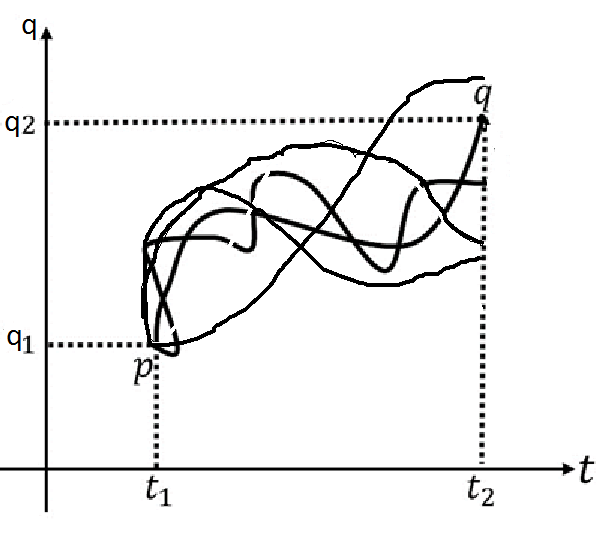
\includegraphics[width=4.66346in,height=4.06736in]{Imagenes/media/image77.png}

\[\delta S = 0 \rightarrow \left. \ \sum_{j}^{}{p_{j}\delta q_{j}} \right\rfloor_{t = t_{2}} = 0\]

Es de recordar que, la acción viene definida por:

\[S = \int_{t_{1}}^{t_{2}}L\left( q_{j},{\dot{q}}_{j};t \right)dt\]

\begin{quote}
\(\frac{dS}{dt} = \int_{t_{1}}^{t_{2}}{\frac{dL}{dt}dt} = L\)+C
\end{quote}

\[\mathbf{p}_{\mathbf{j}}\mathbf{=}\frac{\mathbf{\partial}\mathbf{F}_{\mathbf{2}}\left( \mathbf{q}_{\mathbf{j}}\mathbf{,}\mathbf{P}_{\mathbf{j}}\mathbf{;t} \right)}{\mathbf{\partial}\mathbf{q}_{\mathbf{j}}}\mathbf{,\ \ \ \ \ \ \ \ \ \ \ }\mathbf{Q}_{\mathbf{j}}\mathbf{=}\frac{\mathbf{\partial}\mathbf{F}_{\mathbf{2}}\left( \mathbf{q}_{\mathbf{j}}\mathbf{,}\mathbf{P}_{\mathbf{j}}\mathbf{;t} \right)}{\mathbf{\partial}\mathbf{P}_{\mathbf{j}}}\]

\[\mathbf{p}_{\mathbf{j}}\mathbf{=}\frac{\mathbf{\partial S}\left( \mathbf{q}_{\mathbf{j}}\mathbf{;t} \right)}{\mathbf{\partial}\mathbf{q}_{\mathbf{j}}}\mathbf{,\ \ \ \ \ \ \ \ \ \ \ }\mathbf{Q}_{\mathbf{j}}\mathbf{=}\frac{\mathbf{\partial S}\left( \mathbf{q}_{\mathbf{j}}\mathbf{;t} \right)}{\mathbf{\partial}\mathbf{P}_{\mathbf{j}}}\]

De esta maneta la acción se convierte en función de \(q_{j}\) y \(t\),
es decir que \(S = S\left( q_{j};t \right)\), luego:

\[\frac{dS}{dt} = \sum_{j}^{}{\frac{\partial s}{\partial q_{j}}{\dot{q}}_{j}} + \frac{\partial S}{\partial t} = \sum_{j}^{}{p_{j}{\dot{q}}_{j}} + \frac{\partial S}{\partial t}\]

\[L - \sum_{j}^{}{p_{j}{\dot{q}}_{j}} = \frac{\partial S}{\partial t}\]

\[\mathbf{\ \ \ \ \ \ } - \mathbf{H}\left( \mathbf{q}_{\mathbf{j}}\mathbf{,}\frac{\partial s}{\partial q_{j}}\mathbf{;t} \right) = \frac{\partial S}{\partial t}\]

\[\mathbf{H}\left( \mathbf{q}_{\mathbf{j}}\mathbf{,}\frac{\partial s}{\partial q_{j}}\mathbf{;t} \right)\mathbf{+}\frac{\mathbf{\partial S}}{\mathbf{\partial t}}\mathbf{= 0\ \ \ \ \ \ \ }\]

La ecuación (217) corresponde a la ecuación de Hamilton-Jacobi obtenida
mediante el Principio de Mínima Acción de Hamilton Modificado, en
general:

\[\mathbf{H}\left( \mathbf{q}_{\mathbf{1}}\mathbf{,}\mathbf{q}_{\mathbf{2}}\mathbf{,\ldots,}\mathbf{q}_{\mathbf{n}}\mathbf{,\ }\frac{\mathbf{\partial S}}{\mathbf{\partial}\mathbf{q}_{\mathbf{1}}}\mathbf{,}\frac{\mathbf{\partial S}}{\mathbf{\partial}\mathbf{q}_{\mathbf{2}}}\mathbf{,\ldots,}\frac{\mathbf{\partial S}}{\mathbf{\partial}\mathbf{q}_{\mathbf{n}}}\mathbf{;t} \right)\mathbf{+}\frac{\mathbf{\partial S}}{\mathbf{\partial t}}\mathbf{= 0}\]

Donde \(S\) se llama función principal de Hamilton-Jacobi.

\textbf{Ejemplo 18:} Analizar el problema del oscilador armónico,
utilizando la dinámica de Hamilton-Jacobi.

\textbf{Solución:} El Hamiltoniano para el oscilador armónico está dado
por:

\[H = \frac{p^{2}}{2m} + \frac{1}{2}kq^{2}\]

Llevando este Hamiltoniano a la ecuación de Hamilton-Jacobi, se tiene
que:

\[\mathbf{H}\left( \mathbf{q}_{\mathbf{j}}\mathbf{,}\frac{\partial S}{\partial q_{j}}\mathbf{;t} \right)\mathbf{+}\frac{\mathbf{\partial S}}{\mathbf{\partial t}}\mathbf{= 0\ \ \ \ \ \ \ }\]

\[\frac{1}{2m}\left( \frac{\partial S}{\partial q} \right)^{2} + \frac{1}{2}kq^{2} + \frac{\mathbf{\partial S(q;t)}}{\mathbf{\partial t}}\mathbf{= 0\ \ \ \ \ \ \ }\]

\begin{quote}
\(\frac{1}{2m}\left( \frac{\partial S}{\partial q} \right)^{2} + \frac{1}{2}kq^{2} = \alpha\)=E
\end{quote}

\(\mathbf{\ }\alpha + \frac{\mathbf{\partial S}}{\mathbf{\partial t}}\mathbf{= 0\ \ \ \ \ \ \ }\)

\[S\left( q_{},\alpha;t \right) = w\ (q,\alpha) - \alpha t\]

Usando una nueva función principal de Hamilton-Jacobi \(w\), se va a
cumplir que:

\[\frac{1}{2m}\left( \frac{dw}{dq} \right)^{2} = \alpha - \frac{1}{2}kq^{2}\]

\[dw = \sqrt{\left( \alpha - \frac{1}{2}kq^{2} \right)2m}\ dq\]

De esta manera:

\[w(q,\alpha) = \sqrt{mk}\int_{}^{}\sqrt{\frac{2\alpha}{k} - q^{2}}\ dq\]

\[S\left( q_{j},\alpha;t \right) = \sqrt{mk}\int_{}^{}\sqrt{\frac{2\alpha}{k} - q^{2}}\ dq - \alpha t\]

\(\mathbf{Q}_{\mathbf{j}}\mathbf{=}\frac{\mathbf{\partial S}\left( \mathbf{q}_{\mathbf{j}}\mathbf{;t} \right)}{\mathbf{\partial}\mathbf{P}_{\mathbf{j}}}\)
\(\mathbf{\beta =}\frac{\mathbf{\partial S}\left( \mathbf{q}_{\mathbf{j}}\mathbf{;t} \right)}{\mathbf{\partial\alpha}}\)

\begin{quote}
\(\beta = \frac{\partial S}{\partial\alpha}\ \)=
\(\sqrt{mk}\int_{}^{}\frac{\frac{2}{k}}{2\sqrt{\frac{2\alpha}{k} - q^{2}}}\ dq - t\)

\(\beta + t\ \)=
\(\sqrt{m/k}\int_{}^{}\frac{dq}{\sqrt{\frac{2\alpha}{k} - q^{2}}}\ \)

\(\sqrt{k/m}(\beta + t\ )\)=
\(\int_{}^{}\frac{dq}{\sqrt{\frac{2\alpha}{k} - q^{2}}}\ \)
\end{quote}

Resolviendo:

\[\mathbf{q =}\sqrt{\frac{\mathbf{2}\mathbf{\alpha}}{\mathbf{k}}}\mathbf{sen}{\mathbf{\omega}\left( \mathbf{\beta + t} \right)}\]

\[\mathbf{q =}\sqrt{\frac{\mathbf{2}\mathbf{E}}{\mathbf{m}\mathbf{\omega}^{\mathbf{2}}}}\mathbf{sen}{\mathbf{\omega}\left( \mathbf{\beta + t} \right)}\]

\textbf{DEDUCCIÓN DE LA ECUACIÓN DE SCHRÖDINGER MEDIANTE LA ECUACIÓN DE
HAMILTON-JACOBI}

Para obtener la de ecuación de Schrödinger mediante la ecuación de
Hamilton-Jacobi, se procede a analizar la dinámica de una partícula
libre \(m\) que se mueve bajo la acción de un potencial \(V = u(r)\),
para este caso, el Hamiltoniano va a estar dado por:

\[H = \frac{p^{2}}{2m} + V(r)\]

Por otro lado la ecuación de Hamilton-Jacobi va a estar dada por

\[\mathbf{\ }\mathbf{p}_{\mathbf{j}}\mathbf{=}\frac{\mathbf{\partial S}\left( \mathbf{q}_{\mathbf{j}}\mathbf{;t} \right)}{\mathbf{\partial}\mathbf{q}_{\mathbf{j}}}\]

\[\frac{1}{2m}\left( \frac{\partial S}{\partial r} \right)^{2} + V(r) + \frac{\partial S}{\partial t} = 0\ \ \ \ \ \ \ \ \]

A partir de la ecuación (218) se pretende encontrar la función principal
de Hamilton-Jacobi (acción), para esto se tiene que:

\[\frac{1}{2m}\left( \frac{\partial S}{\partial r} \right)^{2} + V(r) = E\]

Así:

\[E + \frac{\partial S}{\partial t} = 0 \rightarrow \frac{\partial S}{\partial t} = - E\]

De esta manera:

\[S(r,E;t) = w(r,E) - Et\]

\[S(r,E;t) = w(r,E) - Et\]

Por otro lado como:

\[p = \frac{\partial S}{\partial r}\]

\[p = \frac{dw}{dr}\]

Luego:

\[w(r,E) = \overrightarrow{p} \cdot \overrightarrow{r}\]

\[\mathbf{S}\left( \mathbf{r,E;t} \right)\mathbf{=}\overrightarrow{\mathbf{p}}\mathbf{\cdot}\overrightarrow{\mathbf{r}}\mathbf{- Et\ \ \ \ \ \ \ \ \ }\]

La ecuación (219) es el argumento de una función de onda plana.

Considérese ahora el siguiente esquema, el cual representa la evolución
espacial y temporal de una onda plana:

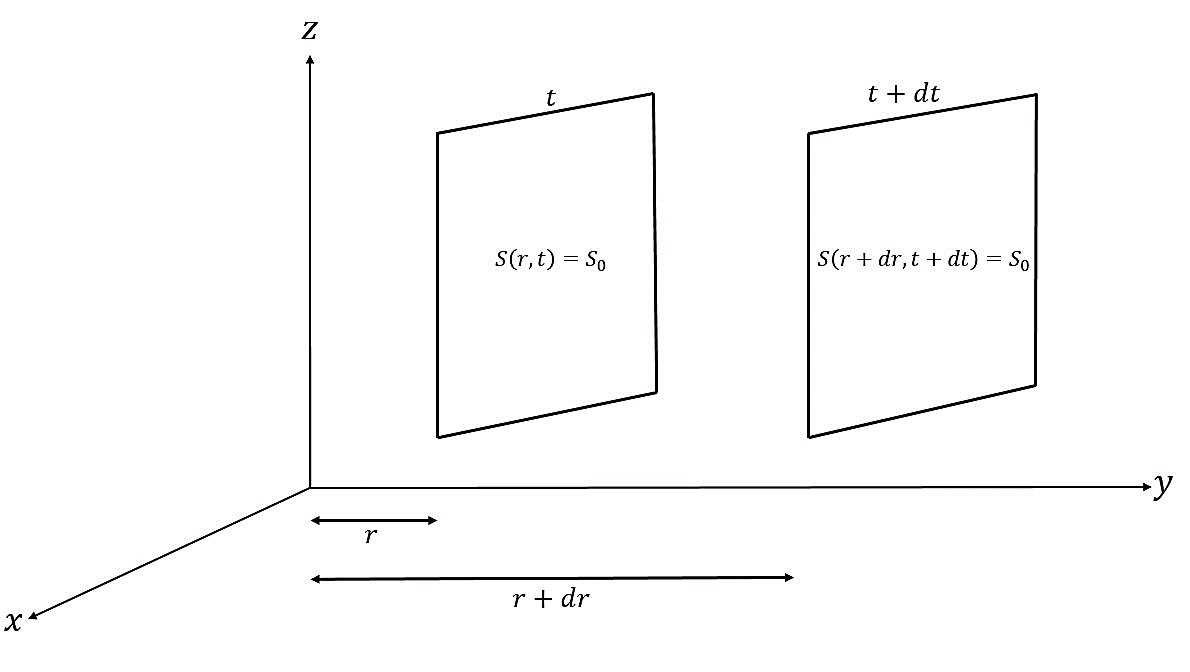
\includegraphics[width=7.01528in,height=3.96111in]{Imagenes/media/image78.png}De
la \emph{figura 52} se tiene que:

\[S(r + dr,t + dt) = S(r,t) + \frac{\partial S}{\partial r}dr + \frac{\partial S}{\partial t}dt\]

\[S_{0} = S_{0} + \overrightarrow{p} \cdot d\overrightarrow{r} - Edt\]

\[\overrightarrow{p} \cdot d\overrightarrow{r} = Edt\]

De donde la velocidad de grupo o velocidad de frente de onda, estará
dada por:

\[\overrightarrow{v} = \frac{E}{\left| \overrightarrow{p} \right|}\widehat{p}\]

Ahora, supóngase que la partícula viaja acompañada de una onda plana,
cuyo argumento es la función principal de Hamilton-Jacobi, así:

\[\psi(r,t) = A(r,t)e^{\frac{i}{}s(r,t)}\ \ \ \ \ \ \ \ \]

La ecuación (220) se denomina función de onda de acción, donde:

\href{http://tex.stackexchange.com/questions/171088/how-can-i-typeset-the-reduced-planck-constant-\%e2\%84\%8f}{\(\mathbf{\hslash}\)}\(\mathbf{=}\frac{h}{2\pi}\)

Y corresponde a la constante de Planck reducida o constante de Dirac.

Ahora se procede a encontrar la ecuación (218) mediante la función de
onda de acción, para esto:

\[\frac{1}{2m}\left( \frac{\partial S}{\partial r} \right)^{2} + V(r) + \frac{\partial S}{\partial t} = 0\ \ \ \ \ \ \ \ \]

\[\psi(r,t) = A(r,t)e^{\frac{i}{}s(r,t)}\ \ \ \ \ \ \ \ \]

\[\frac{\partial\psi(r,t)}{\partial t} = \frac{\partial A(r,t)}{\partial t}e^{\frac{i}{}s(r,t)} + A(r,t)\frac{i}{}\mathbf{\ }\frac{\partial S(r,t)}{\partial t}e^{\frac{i}{}s(r,t)}\]

\[\frac{\partial\psi(r,t)}{\partial t} = \left\lbrack \frac{\partial A}{\partial t} + \frac{i}{}A(r,t)\mathbf{\ }\frac{\partial S(r,t)}{\partial t} \right\rbrack e^{\frac{i}{}s(r,t)}\ \ \ \ \ \ \ \]

Para la parte espacial, se tiene:

\[\frac{\partial\psi(r,t)}{\partial r} = \frac{\partial A}{\partial r}e^{\frac{i}{}s(r,t)} + A(r,t)\frac{i}{}\mathbf{\ }\frac{\partial S(r,t)}{\partial r}e^{\frac{i}{}s(r,t)}\]

\[\frac{\partial\psi(r,t)}{\partial r} = \left\lbrack \frac{\partial A}{\partial r} + \frac{i}{}A(r,t)\mathbf{\ }\frac{\partial S(r,t)}{\partial r} \right\rbrack e^{\frac{i}{}s(r,t)}\ \ \ \ \ \ \ \]

\[\frac{\partial^{2}\psi(r,t)}{\partial r^{2}} = \left( \frac{\partial^{2}A}{\partial r^{2}} + \frac{i}{}\frac{\partial A}{\partial r}\mathbf{\ }\frac{\partial S}{\partial r} + \frac{i}{}A\frac{\partial^{2}S}{\partial r^{2}} \right)e^{\frac{i}{}s(r,t)} + \left( \frac{\partial A}{\partial r} + \frac{i}{}A\frac{\partial S}{\partial r} \right)\frac{i}{}\frac{\partial S}{\partial r}e^{\frac{i}{}s(r,t)}\]

\[\frac{\partial^{2}\psi(r,t)}{\partial r^{2}} = \left\lbrack \nabla^{2}A + \frac{i}{}\frac{\partial A}{\partial r}\mathbf{\ }\frac{\partial S}{\partial r} + \frac{i}{}A\frac{\partial^{2}S}{\partial r^{2}} + \frac{i}{}\frac{\partial A}{\partial r}\frac{\partial S}{\partial r} - \frac{1}{\hslash^{2}}A\left( \frac{\partial S}{\partial r} \right)^{2} \right\rbrack e^{\frac{i}{}s(r,t)}\]

\[\frac{\partial^{2}\psi(r,t)}{\partial r^{2}} = \left\lbrack \nabla^{2}A + 2\frac{i}{}\frac{\partial A}{\partial r}\mathbf{\ }\frac{\partial S}{\partial r} + \frac{i}{}A\frac{\partial^{2}S}{\partial r^{2}} - \frac{1}{\hslash^{2}}A\left( \frac{\partial S}{\partial r} \right)^{2} \right\rbrack e^{\frac{i}{}s(r,t)}\]

\[\frac{\partial^{2}\psi(r,t)}{\partial r^{2}} = \left\lbrack \nabla^{2}A - \frac{1}{\hslash^{2}}A\left( \frac{\partial S}{\partial r} \right)^{2} + \frac{i}{}\frac{1}{A}\frac{\partial}{\partial r}\left( A^{2}\frac{\partial S}{\partial r} \right)\mathbf{\ } \right\rbrack e^{\frac{i}{}s(r,t)}\ \ \ \ \ \ \]

\[\frac{\partial\psi(r,t)}{\partial t} = \left\lbrack \frac{1}{A}\frac{\partial A}{\partial t} + \frac{i}{}\mathbf{\ }\frac{\partial S(r,t)}{\partial t} \right\rbrack A(r,t)e^{\frac{i}{}s(r,t)}\ \ \ \ \ \ \ \]

\[\frac{\partial^{2}\psi(r,t)}{\partial r^{2}} = \left\lbrack \frac{\nabla^{2}A}{A} - \frac{1}{\hslash^{2}}\left( \frac{\partial S}{\partial r} \right)^{2} + \frac{i}{}\frac{1}{A^{2}}\frac{\partial}{\partial r}\left( A^{2}\frac{\partial S}{\partial r} \right)\mathbf{\ } \right\rbrack{A(r,t)e}^{\frac{i}{}s(r,t)}\]

\[\frac{1}{2m}\left( \frac{\partial S}{\partial r} \right)^{2} + V(r) + \frac{\partial S}{\partial t} = 0\ \ \ \ \ \ \ \ \]

\[- \frac{\hslash^{2}}{2m}\frac{\partial^{2}\psi(r,t)}{\partial r^{2}} + V(r)\psi(r,t) - i\hslash\frac{\partial\psi(r,t)}{\partial t} =\]

\[\left\lbrack - \frac{{}^{2}}{2m}\frac{\nabla^{2}A}{A} + \frac{1}{2m}\left( \frac{\partial S}{\partial r} \right)^{2} - \frac{i}{}\frac{{}^{2}}{2m}\frac{1}{A^{2}}\frac{\partial}{\partial r}\left( A^{2}\frac{\partial S}{\partial r} \right)\  \right\rbrack Ae^{\frac{i}{}s(r,t)} + V(r)Ae^{\frac{i}{}s(r,t)} + \left( - \frac{i}{A}\frac{\partial A}{\partial t} + \frac{\partial S}{\partial t} \right){Ae}^{\frac{i}{}s(r,t)}\]

\[- \frac{\hslash^{2}}{2m}\frac{\partial^{2}\psi(r,t)}{\partial r^{2}} + V(r)\psi(r,t) - i\hslash\frac{\partial\psi(r,t)}{\partial t} =\]

\[\left\{ \frac{1}{2m}\left( \frac{\partial S}{\partial r} \right)^{2} + V(r) + \frac{\partial S}{\partial t} - \frac{{}^{2}}{2m}\frac{\nabla^{2}A}{A} - \frac{i}{2}\frac{1}{A^{2}}\ \left\lbrack \frac{\partial}{\partial r}\left( \frac{A^{2}}{m}\frac{\partial S}{\partial r} \right) + \frac{\partial}{\partial t}\left( A^{2} \right) \right\rbrack \right\} A(r,t)e^{\frac{i}{}s(r,t)}\]

\[- \frac{\hslash^{2}}{2m}\frac{\partial^{2}\psi(r,t)}{\partial r^{2}} + V(r)\psi(r,t) - i\hslash\frac{\partial\psi(r,t)}{\partial t} = 0\  + j0\ \ \ \ \]

\[\frac{1}{2m}\left( \frac{\partial S}{\partial r} \right)^{2} + V(r) + \frac{\partial S}{\partial t} - \frac{{}^{2}}{2m}\frac{\nabla^{2}A}{A} = 0\]

\[\frac{1}{2m}\left( \frac{\partial S}{\partial r} \right)^{2} + V(r) + \frac{\partial S}{\partial t} = \frac{{}^{2}}{2m}\frac{\nabla^{2}A}{A}\]

\[\frac{\partial}{\partial r}\left( \frac{A^{2}}{m}\frac{\partial S}{\partial r} \right) + \frac{\partial}{\partial t}\left( A^{2} \right) = 0\]

\[A^{2} = \rho(r;t)\]

\[\frac{1}{m}\frac{\partial S}{\partial r} = \overrightarrow{v}(r;t)\]

\[\frac{1}{2m}\left( \frac{\partial S}{\partial r} \right)^{2} + V(r) + \frac{\partial S}{\partial t} = \frac{{}^{2}}{2m}\frac{\nabla^{2}A}{A}\]

\(\nabla.\overrightarrow{J} + \frac{\partial\rho(r;t)}{\partial t} = 0\)

La ecuación (224) es la famosa ECUACIÓN DE SCHRÖDINGER la cual juega un
papel fundamental en la mecánica cuántica.

\[- \frac{\hslash^{2}}{2m}\frac{\partial^{2}\psi(r,t)}{\partial r^{2}} + V(r)\psi(r,t) - i\hslash\frac{\partial\psi(r,t)}{\partial t} = 0\ \ \ \ \ \ \]

\end{document}
